\documentclass[justified]{tufte-book}

% ams
\usepackage{amssymb,amsmath}

\usepackage{ifxetex,ifluatex}
\usepackage{fixltx2e} % provides \textsubscript
\ifnum 0\ifxetex 1\fi\ifluatex 1\fi=0 % if pdftex
  \usepackage[T1]{fontenc}
  \usepackage[utf8]{inputenc}
\else % if luatex or xelatex
  \makeatletter
  \@ifpackageloaded{fontspec}{}{\usepackage{fontspec}}
  \makeatother
  \defaultfontfeatures{Ligatures=TeX,Scale=MatchLowercase}
  \makeatletter
  \@ifpackageloaded{soul}{
     \renewcommand\allcapsspacing[1]{{\addfontfeature{LetterSpace=15}#1}}
     \renewcommand\smallcapsspacing[1]{{\addfontfeature{LetterSpace=10}#1}}
   }{}
  \makeatother

\fi

% graphix
\usepackage{graphicx}
\setkeys{Gin}{width=\linewidth,totalheight=\textheight,keepaspectratio}

% booktabs
\usepackage{booktabs}

% url
\usepackage{url}

% hyperref
\usepackage{hyperref}

% units.
\usepackage{units}


\setcounter{secnumdepth}{2}

% citations

% pandoc syntax highlighting

% longtable
\usepackage{longtable,booktabs}

% multiplecol
\usepackage{multicol}

% strikeout
\usepackage[normalem]{ulem}

% morefloats
\usepackage{morefloats}


% tightlist macro required by pandoc >= 1.14
\providecommand{\tightlist}{%
  \setlength{\itemsep}{0pt}\setlength{\parskip}{0pt}}

% title / author / date
\title{Odds \& Ends}
\author{Jonathan Weisberg}
\date{}

%\usepackage{MinionPro}
%\usepackage{fontspec}
%\newfontfamily\DejaSans{DejaVu Sans}

\newcommand{\given}{\mid}
\renewcommand{\neg}{\mathbin{\sim}}
\renewcommand{\wedge}{\mathbin{\&}}
\renewcommand{\u}{U}
\newcommand{\gt}{>}
\newcommand{\p}{Pr}
\newcommand{\E}{E}
\newcommand{\EU}{EU}
\newcommand{\pr}{Pr}
\newcommand{\po}{Pr^*}
\definecolor{bookred}{RGB}{228,6,19}
\definecolor{bookblue}{RGB}{0,92,169}
\definecolor{bookpurple}{RGB}{114,49,94}

\newenvironment{epigraph}%
{
\begin{flushright}    
\begin{minipage}{20em}
\begin{flushright}
\itshape
}%
{
\end{flushright}
\end{minipage}
\end{flushright}
}
\newenvironment{problem}{\begin{quote}\normalsize}{\end{quote}}
\newenvironment{puzzle}{\begin{quote}\normalsize}{\end{quote}}
\newenvironment{argument}{\begin{quote}\normalsize}{\end{quote}}
\usepackage{fontawesome}
\newenvironment{warning}{\begin{itemize}\item[\faBan]}{\end{itemize}}
\usepackage{marvosym}
\newenvironment{info}{\begin{itemize}\item[\Info]}{\end{itemize}}

%%%% Kevin Godny's code for title page and contents from https://groups.google.com/forum/#!topic/tufte-latex/ujdzrktC1BQ
\makeatletter
\renewcommand{\maketitlepage}{%
\begingroup%
\setlength{\parindent}{0pt}
{\fontsize{18}{18}\selectfont\textit{\@author}\par}
\vspace{1.75in}{\fontsize{36}{14}\selectfont\@title\par}
\vspace{0.5in}{\fontsize{20}{14}\selectfont Introducing Probability \& Decision with a Visual Emphasis\par}
\vspace{0.5in}{\fontsize{14}{14}\selectfont\textsf{\smallcaps{v0.1 beta}}\par}
\vfill{\fontsize{14}{14}\selectfont\textit{An Open Access Publication}\par}
\thispagestyle{empty}
\endgroup
}
\makeatother

% Change shape from [display] to [block] to keep chapter numbers and titles on the same line
\titleformat{\chapter}%
  [block]% shape
  {\relax\ifthenelse{\NOT\boolean{@tufte@symmetric}}{\begin{fullwidth}}{}}% format applied to label+text
  {\itshape\huge\thechapter}% label
  {3em}% horizontal separation between label and title body
  {\huge\rmfamily\itshape}% before the title body
  [\ifthenelse{\NOT\boolean{@tufte@symmetric}}{\end{fullwidth}}{}]% after the title body


\usepackage{etoolbox}
% Jesse Rosenthal's code from https://groups.google.com/forum/#!topic/pandoc-discuss/wCF78X6SvwY
% Avoid new pagraph/indent after lists, quotes, etc.
\makeatletter
\newcommand{\gobblepars}{% 
    \@ifnextchar\par% 
        {\expandafter\gobblepars\@gobble}% 
        {}}
\newcommand{\eatpar}{\@ifnextchar\par{\@gobble}{}}
\newcommand{\forcepar}{\par}
\makeatother
\AfterEndEnvironment{quote}{\expandafter\gobblepars}
\AfterEndEnvironment{enumerate}{\expandafter\gobblepars}
\AfterEndEnvironment{itemize}{\expandafter\gobblepars}
\AfterEndEnvironment{description}{\expandafter\gobblepars}
\AfterEndEnvironment{example}{\expandafter\gobblepars}
\AfterEndEnvironment{argument}{\expandafter\gobblepars}
\AfterEndEnvironment{problem}{\expandafter\gobblepars}
\AfterEndEnvironment{info}{\expandafter\gobblepars}
\AfterEndEnvironment{warning}{\expandafter\gobblepars}
\AfterEndEnvironment{longtable}{\expandafter\gobblepars} % not working, why?


% prevent extra space when \newthought follows \section
% see: https://tex.stackexchange.com/questions/291746/tufte-latex-newthought-after-section
\makeatletter
\def\tuftebreak{%
  \if@nobreak\else
    \par
    \ifdim\lastskip<\tufteskipamount
      \removelastskip \penalty -100
      \tufteskip
    \fi
  \fi
}
\makeatother

% indent lists a bit
\usepackage{enumitem}
\setlist[1]{leftmargin=24pt}

\usepackage{amsthm}
\newtheorem{theorem}{Theorem}[chapter]
\newtheorem{lemma}{Lemma}[chapter]
\theoremstyle{definition}
\newtheorem{definition}{Definition}[chapter]
\newtheorem{corollary}{Corollary}[chapter]
\newtheorem{proposition}{Proposition}[chapter]
\theoremstyle{definition}
\newtheorem{example}{Example}[chapter]
\theoremstyle{definition}
\newtheorem{exercise}{Exercise}[chapter]
\theoremstyle{remark}
\newtheorem*{remark}{Remark}
\newtheorem*{solution}{Solution}
\let\BeginKnitrBlock\begin \let\EndKnitrBlock\end
\begin{document}

\maketitle



{
\setcounter{tocdepth}{1}
\tableofcontents
}

\hypertarget{preface}{%
\chapter*{Preface}\label{preface}}
\addcontentsline{toc}{chapter}{Preface}

\newthought{This} textbook is for introductory philosophy courses on
probability and inductive logic. It is based on a typical such course I
teach at the University of Toronto, where we offer ``Probability \&
Inductive Logic'' in the second year, alongside the usual deductive
logic intro.\(\,\)

The book assumes no deductive logic. The early chapters introduce the
little that's used. In fact almost no formal background is presumed,
only very simple high school algebra.

Several well known predecessors inspired and shaped this book. Brian
Skyrms' \emph{Choice \& Chance} and Ian Hacking's \emph{An Introduction
to Probability and Inductive Logic} were especially influential. Both
texts are widely used with good reason---they are excellent. I've taught
both myself many times, with great success. But this book blends my
favourite aspects of each, organizing them in the sequence and style I
prefer.

I hope this book also offers more universal benefits:

\begin{enumerate}
\def\labelenumi{\arabic{enumi}.}
\tightlist
\item
  It is open access, hence free.
\item
  It's also \href{https://github.com/jweisber/vip-source}{open source},
  so other instructors can modify it to their liking.
\item
  It's available in both
  \href{http://jonathanweisberg.org/vip/_main.pdf}{PDF} and
  \href{http://jonathanweisberg.org/vip/}{HTML}. So it can be read
  comfortably on a range of devices, or printed.
\item
  It emphasizes visual explanations and techniques, to make the material
  more approachable.
\item
  It livens up the text with hyperlinks, images, and margin notes that
  highlight points of history and curiosity. I also hope to add some
  animations and interactive tools soon.
\end{enumerate}

\newthought{The} book is divided into three main parts. The first
explains the basics of logic and probability, the second covers basic
decision theory, and the last explores the philosophical foundations of
probability and statistics. This last, philosophical part focuses on the
Bayesian and frequentist approaches.

A ``cheat sheet'' summarizing key definitions and formulas appears in
\protect\hyperlink{cheat-sheet}{Appendix}
\protect\hyperlink{cheat-sheet}{A}. Further appendices cover the
axiomatic construction of probability theory, Hume's problem of
induction, and Goodman's new ridle of induction.

\newthought{I} usually get a mix of students in my course, with
different ideological inclinations and varying levels of background. For
some the technical material is easy, even review. For others, a healthy
skepticism about scientific methods and discourses comes naturally. My
goal is to get these students all more or less on the same page.

By the end of the course, students with little formal background have a
bevy of tools for thinking about uncertainty. They can understand much
more of the statistical and scientific discourse they encounter. And
hopefully they have a greater appreciation for the value of formal
methods. Students who already have strong formal tools and skills will,
I hope, better understand their limitations. I want them to understand
why these tools leave big questions open---not just philosophically, but
also in very pressing, practical ways.

\newthought{The} book was made with the \texttt{bookdown} package
created by Yihui Xie. It's a wonderful tool, built on a bunch of other
technologies I love, especially the R programming language and the
pandoc conversion tool created by philosopher John MacFarlane. The
book's visual style emulates the famous designs of Edward Tufte, thanks
to more software created by Yihui Xie, J. J. Allaire, and many others
who adapted Tufte's designs to HTML and PDF (via LaTeX).

If it weren't for these tools, I never would have written this book. It
wouldn't have been possible to create one that does all the things this
book is meant to do. I also owe inspiration to Kieran Healy's book
\href{http://socviz.co/}{\emph{Data Visualization: A Practical
Introduction}}, which uses the same suite of tools. It gave me the idea
to use those tools for an updated, open, and visually enhanced rendition
of the classic material from Skyrms and Hacking.

\hypertarget{part-part-i}{%
\part*{Part I}\label{part-part-i}}
\addcontentsline{toc}{part}{Part I}

\hypertarget{the-monty-hall-problem}{%
\chapter{The Monty Hall Problem}\label{the-monty-hall-problem}}

\begin{epigraph}
\ldots{}in no other branch of mathematics is it so easy for experts to
blunder as in probability theory.\\
---Martin Gardner
\end{epigraph}

\newthought{Imagine} you're on a game show. There are three doors, one
with a prize behind it. You're allowed to pick any door, so you choose
the first one at random, door A.

\begin{marginfigure}
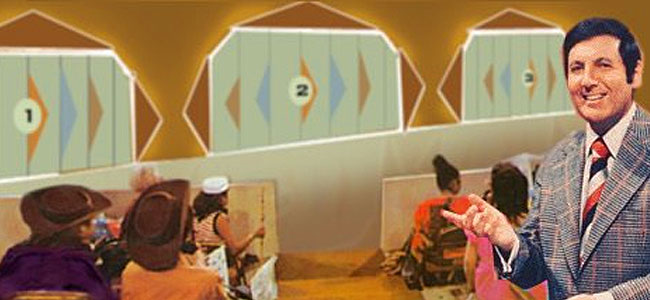
\includegraphics{img/lets_make_a_deal.png} The Monty Hall problem is
named after the creator and host of the game show \emph{Let's Make a
Deal}.
\end{marginfigure}

Now the rules of the game require the host to open one of the other
doors and let you switch your choice if you want. Because the host
doesn't want to give away the game, they always open an empty door.

In your case, the host opens door C: no prize, as expected. ``Do you
want to switch to door B?'', the host asks.

Pause a moment to think about your answer before reading on.

\newthought{What} did you decide? Did you conclude it doesn't matter
whether you stick with door A or switch to door B?

\begin{marginfigure}
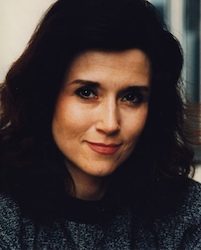
\includegraphics{img/marilyn_vos_savant.png} Marilyn vos Savant made the
Monty Hall problem famous when she solved it correctly in her ``Ask
Marilyn'' column for \emph{Parade} magazine. Read more about it in
\href{https://www.nytimes.com/1991/07/21/us/behind-monty-hall-s-doors-puzzle-debate-and-answer.html}{\emph{The
New York Times}}.
\end{marginfigure}

If so, you're in good company. Most people find this answer sensible,
including some professors of statistics and mathematics. They figure
there are only two possibilities remaining, door A and door B, each with
the same one-in-two chance of being the winner. So it doesn't matter
which one you pick.

But the right answer is you should switch. Door B is now twice as likely
to be the winner as door A. Why?

The reason is subtle. One way to think about it is that the host's
choice of which door to open is a bit of a tell. Maybe they \emph{had}
to open door C, because the prize is behind door B and they didn't want
to give that away. Of course, it could be behind door A instead, so
maybe they just picked door C at random. But there was only a
one-in-three chance the prize would be behind door A. Which means
there's a two-in-three chance they didn't really have a choice, they had
to open door C to avoid showing you the prize behind door B.

\begin{marginfigure}
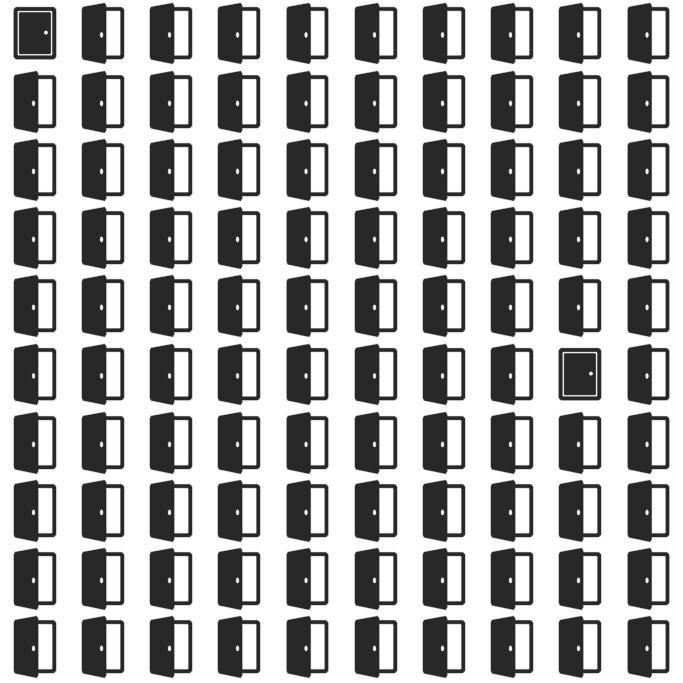
\includegraphics{_main_files/figure-latex/montygrid-1} \caption[The hundred-door version of the Monty Hall problem, suggested by Marilyn vos Savant]{The hundred-door version of the Monty Hall problem, suggested by Marilyn vos Savant}\label{fig:montygrid}
\end{marginfigure}

Here's another way to think about it. Imagine the game had a hundred
doors instead of just three. And suppose again you start by picking the
first door at random. Then the host opens \emph{all the other doors but
one}, door \(59\) let's say. You have to ask yourself: why did they pick
door \(59\) to leave closed?? Almost certainly because that's where the
prize is hidden! Maybe you got really lucky and picked right with the
first door at the beginning. But it's way more likely you didn't, and
the host had to keep door \(59\) closed to avoid giving away the game.

\hypertarget{diagramming-the-solution}{%
\section{Diagramming the Solution}\label{diagramming-the-solution}}

\begin{marginfigure}
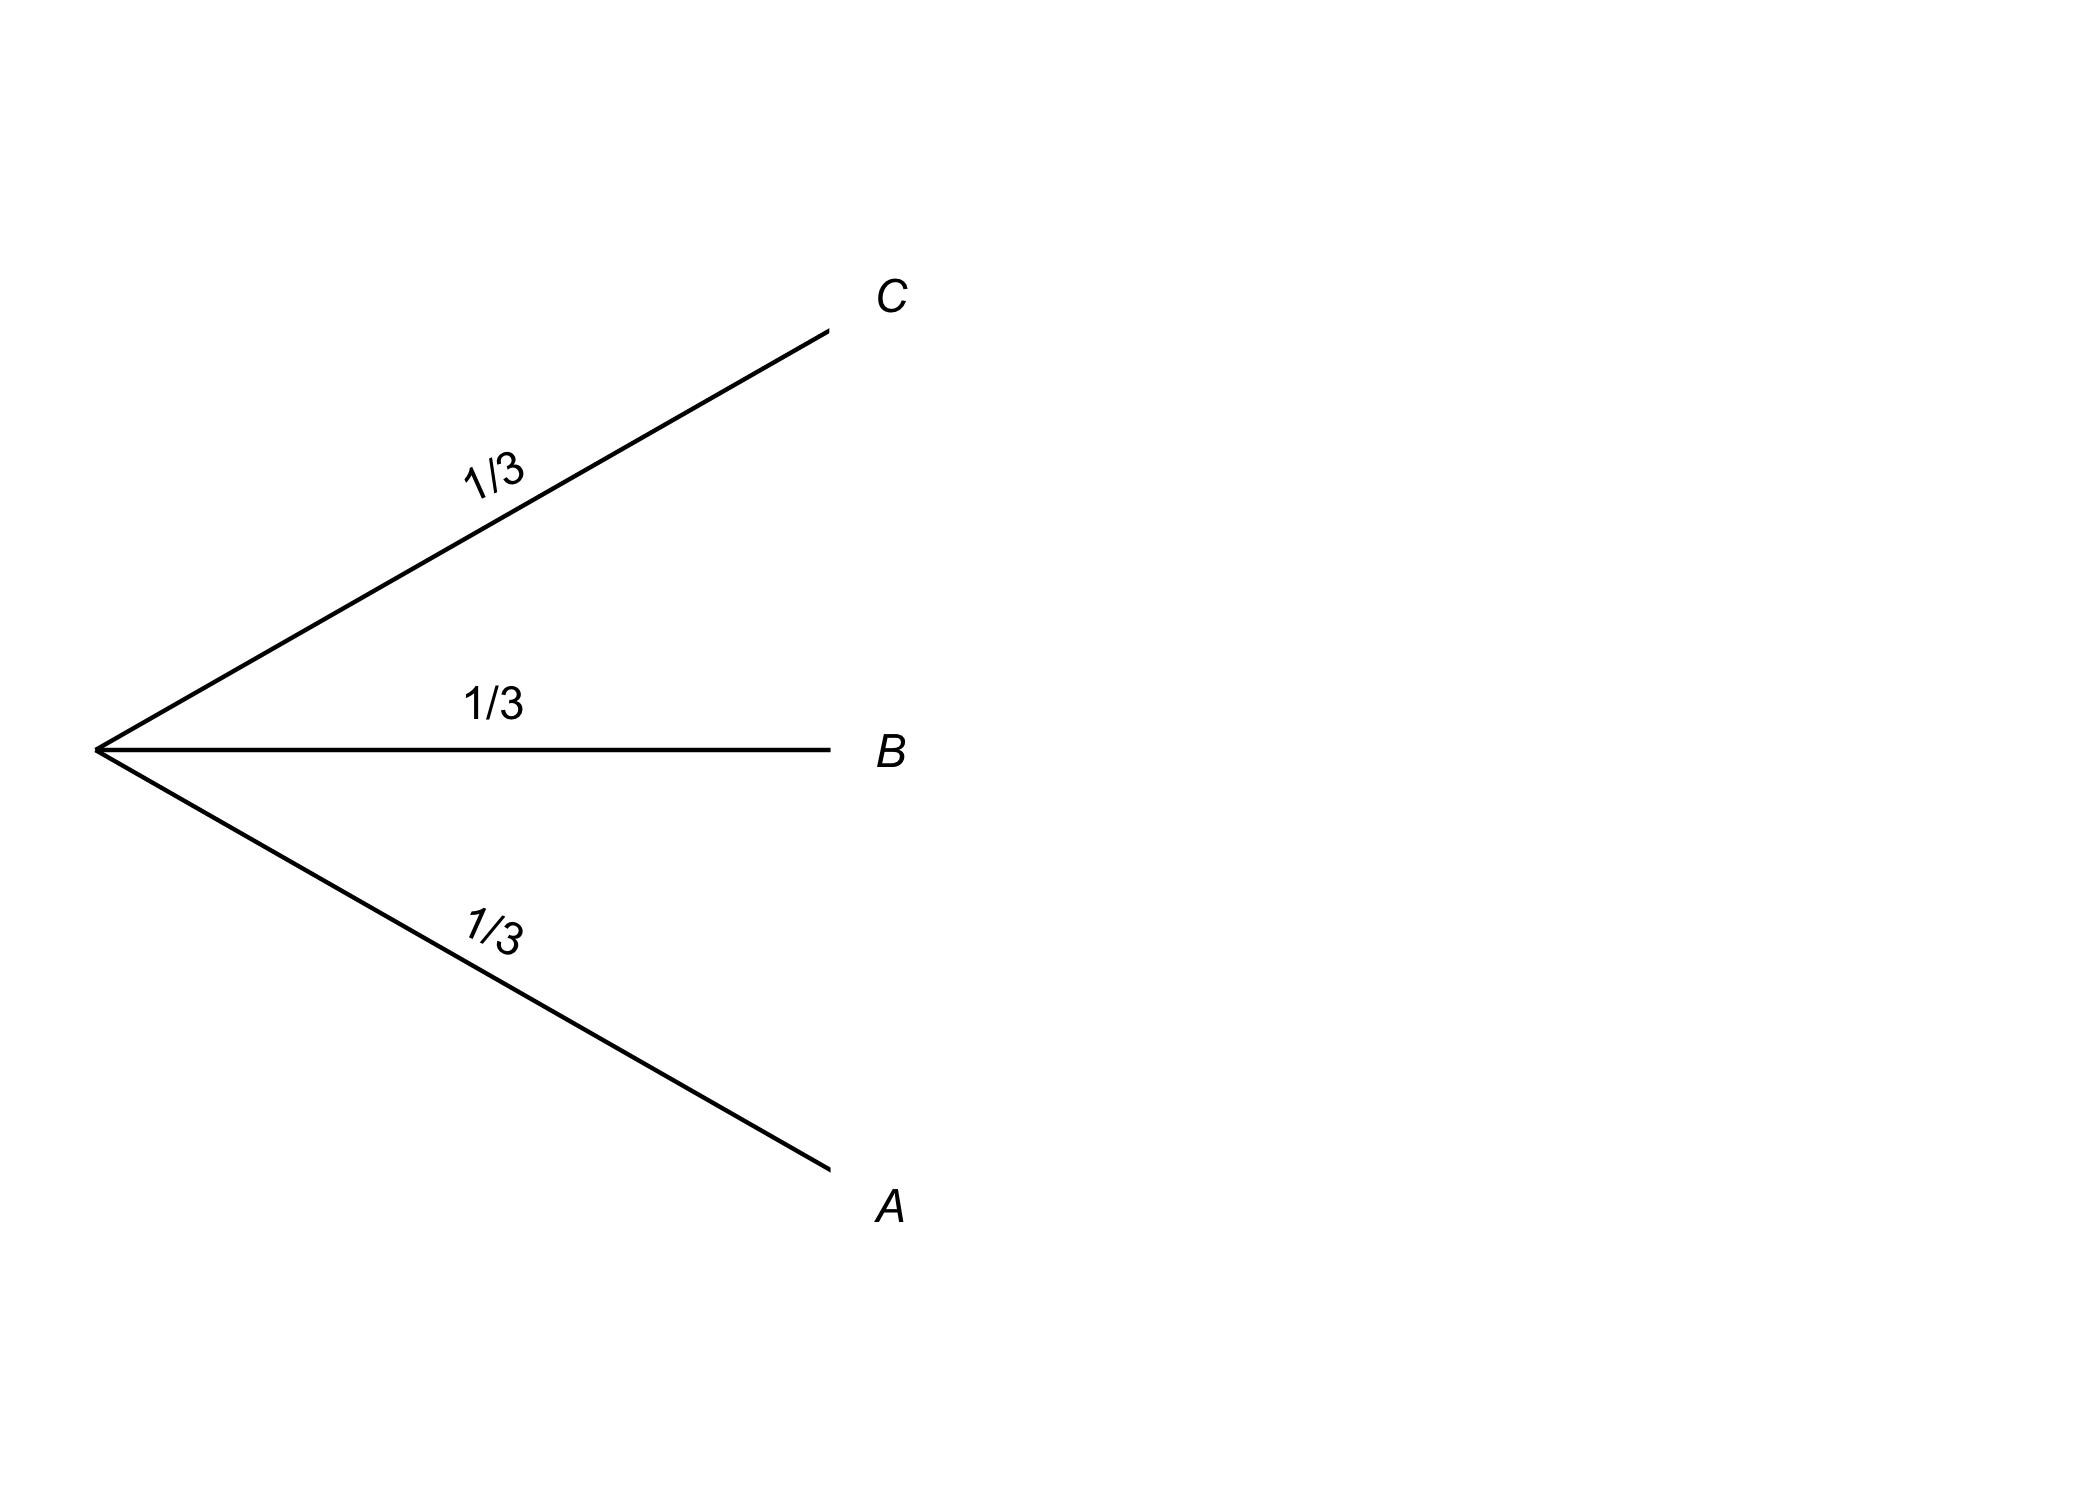
\includegraphics{_main_files/figure-latex/montytree1-1} \caption[First stage of a tree diagram for the Monty Hall problem]{First stage of a tree diagram for the Monty Hall problem}\label{fig:montytree1}
\end{marginfigure}
\begin{marginfigure}
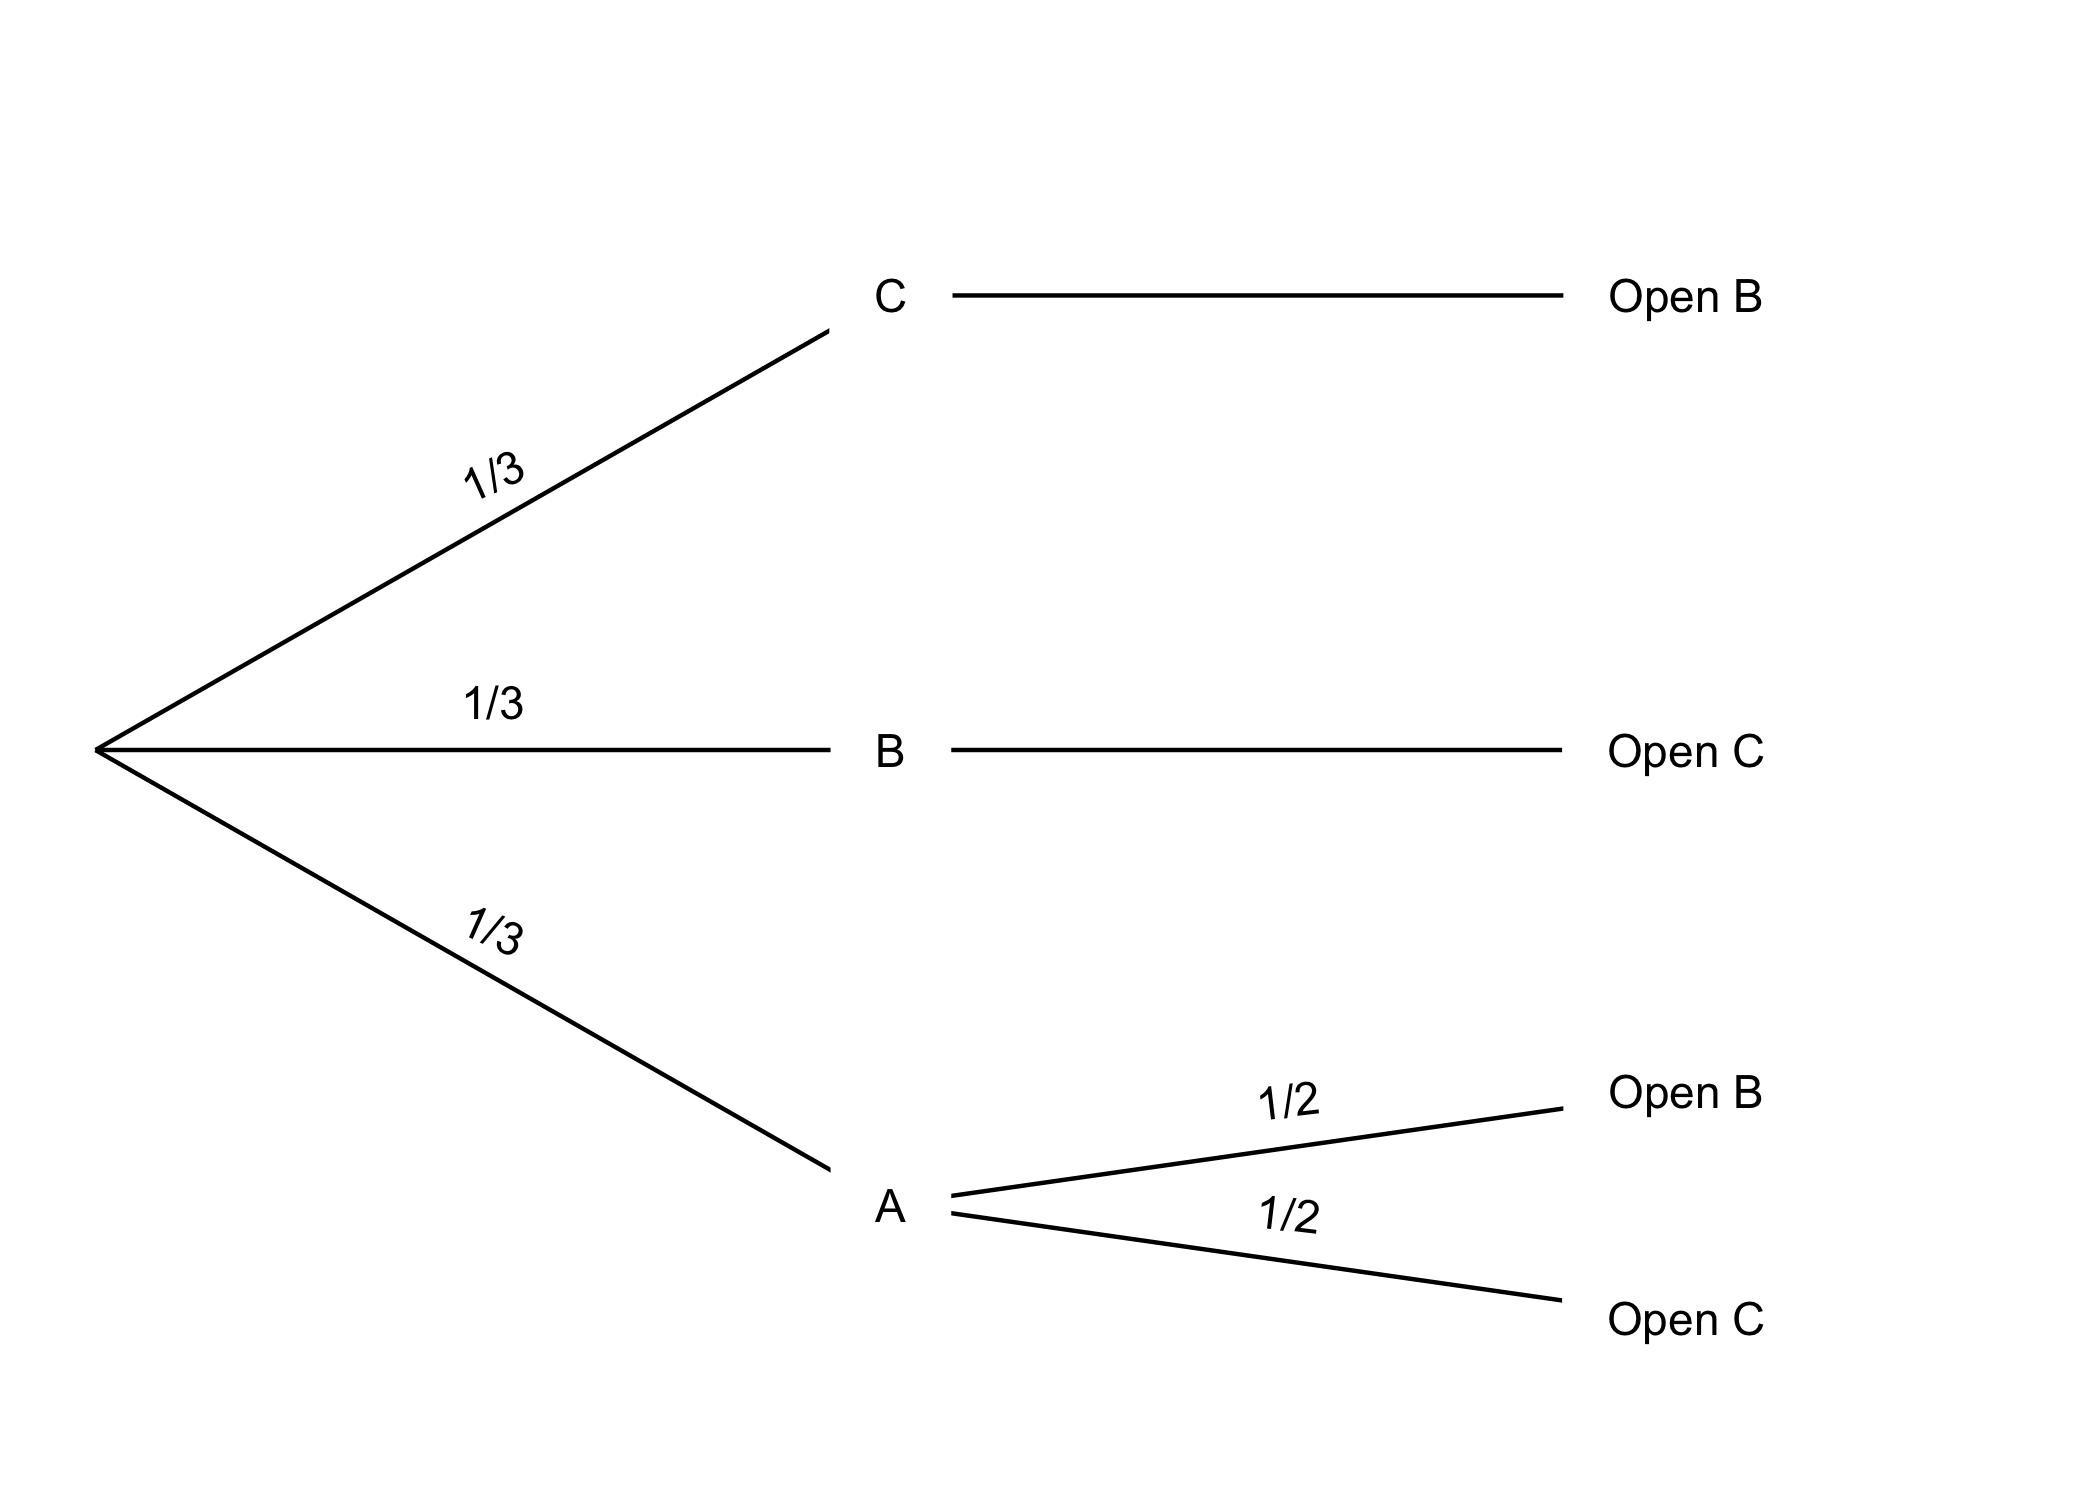
\includegraphics{_main_files/figure-latex/montytree2-1} \caption[Second stage]{Second stage}\label{fig:montytree2}
\end{marginfigure}
\begin{marginfigure}
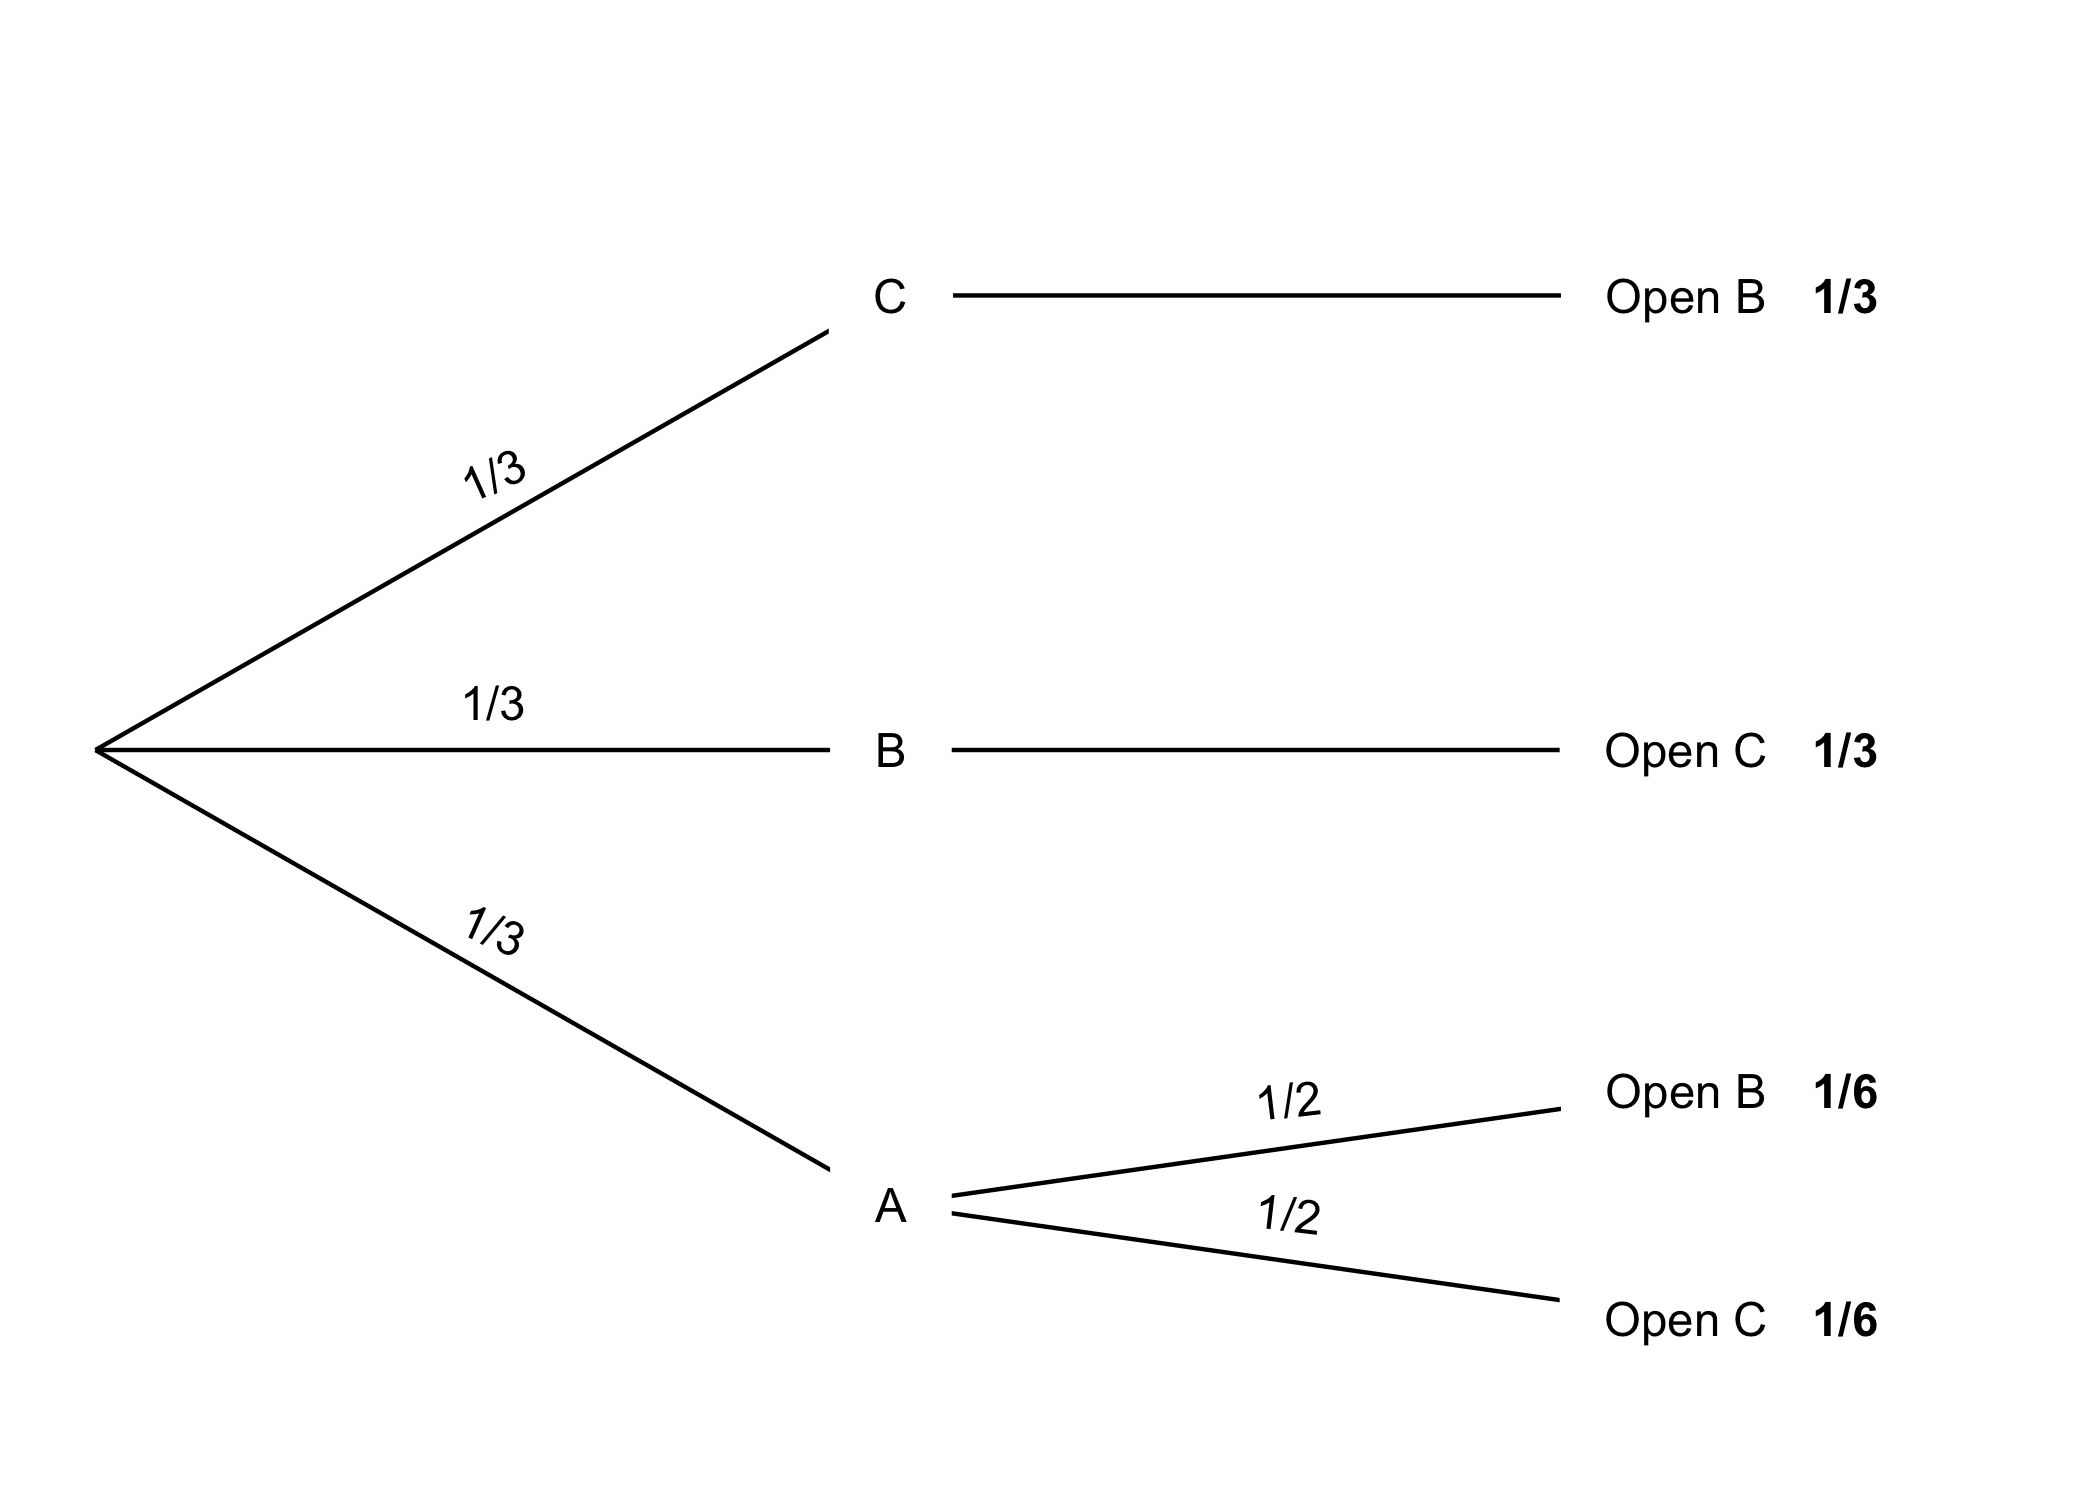
\includegraphics{_main_files/figure-latex/montytree3-1} \caption[Third and final stage]{Third and final stage}\label{fig:montytree3}
\end{marginfigure}

\newthought{A} picture helps clarify things. At first the prize could be
behind any of the three doors, with equal probability each way. So we
draw a tree with three branches, each labeled with a probability of
\(1/3\). Figure \ref{fig:montytree1} shows the result.

Now, which door the host opens may depend on where the prize is,
i.e.~which branch we're on. If it's behind door C, they won't show you
by opening that door. They would have to open door B in this case.

Likewise, if the prize is behind door C, then opening door B is their
only option.

Only if the prize is behind door A do they have a choice: open either
door B or door C. In that case it's a tossup which door they'll open, so
each of those possibilities has a 1/2 chance. Check out Figure
\ref{fig:montytree2}.

Now imagine playing the game over and over. A third of the time things
will follow the top path; a third of the time they'll follow the middle
one; and the remaining third they'll follow one of the two bottom paths.

When things follow the bottom branches, half of those times the host
will open door B, and half the time they'll open door C. So one in every
six plays will follow the \emph{A-and-Open-B} path. And one in every six
plays will follow the \emph{A-and-Open-C} path. See Figure
\ref{fig:montytree3}.

Now we can understand what happens when the host opens door C. Usually
it's because the prize is behind door B. Sometimes they open door C
because the prize is behind door A instead. But that's only a sixth of
the time, compared to a third of the time where they open door C because
the prize is behind door B.

So when you see the host open door C, you should think it's more likely
you're on the middle branch, with the prize behind door B. Switch!

\hypertarget{lessons}{%
\section{Lessons Learned}\label{lessons}}

\newthought{Tree} diagrams are a handy tool for solving probability
problems. They also illustrate some central concepts of probability.

Probabilities are numbers assigned to possibilities. In the Monty Hall
problem, there are three possibilities for where the prize is: door A,
door B, and door C. Each of these possibilities has the same
probability: 1/3.

\newthought{Some} possibilities are \textbf{\emph{mutually exclusive}},
meaning only one of them can obtain. The prize can't be behind door A
and door B, for example. Here are more examples of mutually exclusive
possibilities:

\begin{itemize}
\tightlist
\item
  A coin can land heads or tails, but it can't do both on the same toss.
\item
  A card drawn from a standard deck could be either an ace or a queen,
  but it can't be both.
\item
  The temperature at noon tomorrow could be 20 degrees, or it could be
  25 degrees, but it can't be both.
\end{itemize}

When possibilities are mutually exclusive, their probabilities add up.
For example, the initial probability the prize will be behind either
door A or door B is \(1/3 + 1/3 = 2/3\). And the probability a card
drawn from a standard deck will be either an ace or a queen is
\(4/52 + 4/52 = 8/52 = 2/13\).

\newthought{Another} key concept is possibilities that are
\textbf{\emph{exhaustive}}. In the Monty Hall problem, the prize has to
be behind one of the three doors, so A, B, and C ``exhaust'' all the
possibilities. Here are more examples of exhaustive possibilities:

\begin{itemize}
\tightlist
\item
  A card drawn from a standard deck must be either red or black.
\item
  The temperature at noon tomorrow must be either above zero, below
  zero, or zero.
\end{itemize}

\begin{marginfigure}
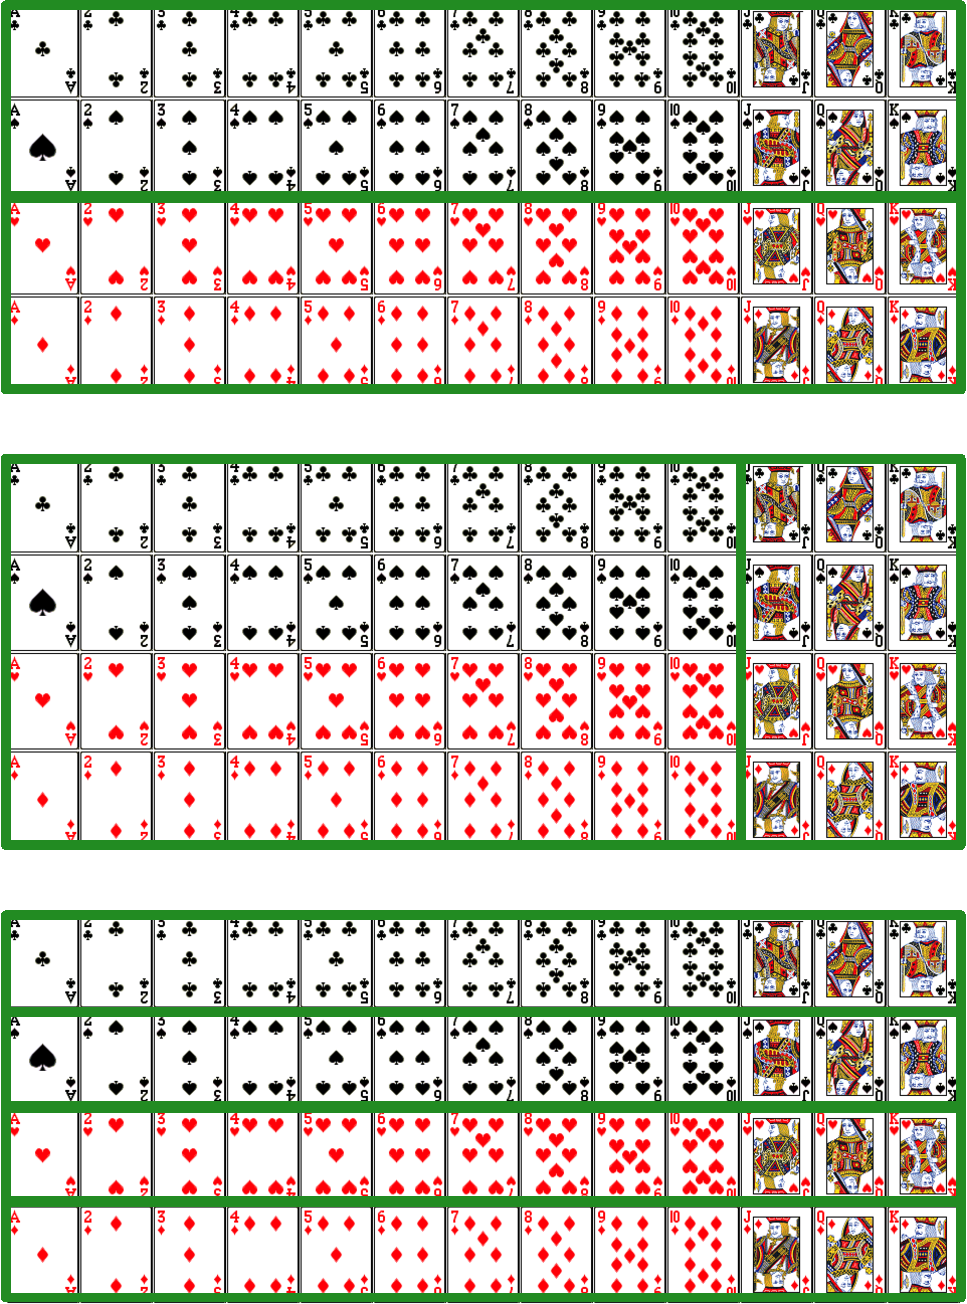
\includegraphics{_main_files/figure-latex/unnamed-chunk-4-1} \caption[Three  partitions for a card drawn from a standard deck]{Three  partitions for a card drawn from a standard deck}\label{fig:unnamed-chunk-4}
\end{marginfigure}

\newthought{In} our tree diagrams, each branch-point always uses a set
of possibilities that is \emph{both} exclusive \emph{and} exhaustive.
The first split on the three doors covers all the possibilities for
where the prize might be, and only one of those possibilities can be the
actual location of the prize. Likewise for the second stage of the
diagram. On the bottom branch for example, the host must open either
door B or door C given the rules, but he will only open one or the
other.

When a set of possibilities is both exclusive and exhaustive, it's
called a \textbf{\emph{partition}}. A partition ``carves up'' the space
of possibilities into distinct, non-overlapping units.

There can be more than one way to partition the space of possibilities.
For example, a randomly drawn playing card could be black or red; it
could be a face card or not; and it could be any of the four suits
(\(\heartsuit\), \(\diamondsuit\), \(\clubsuit\), \(\spadesuit\)).

\newthought{When} possibilities form a partition, their probabilities
must add up to 1. Initially, the probability the prize will be behind
one of the three doors is \(1/3 + 1/3 + 1/3 = 1\). And the probability
that a card drawn from a standard deck at random will be either red or
black is \(1/2 + 1/2 = 1\).

In a way, the fundamental principle of probability is that probabilities
over a partition must add up to 1.

\newthought{Tree} diagrams follow a few simple rules based on these
concepts. The parts of a tree are called \emph{nodes}, \emph{branches},
and \emph{leaves}: see Figure \ref{fig:treeparts}.

\begin{figure}
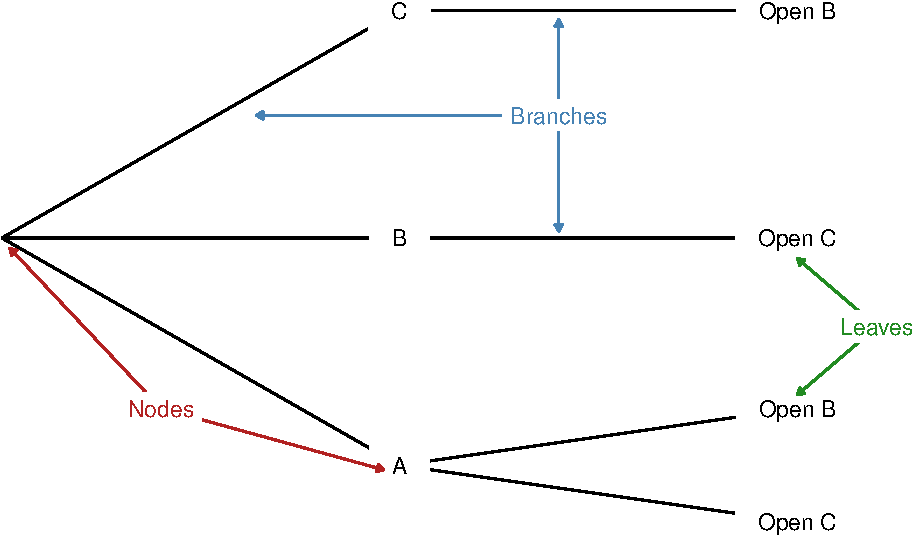
\includegraphics{_main_files/figure-latex/treeparts-1} \caption[The parts of a tree diagram]{The parts of a tree diagram: nodes, branches, and leaves}\label{fig:treeparts}
\end{figure}

The rules for a tree are as follows:

\emph{Rule 1.} Each node must use a partition. The branches coming out
of it must be mutually exclusive possibilities, and they must cover all
the possibilities.

\emph{Rule 2.} The probabilities at each node must add up to \(1\).

\emph{Rule 3.} The probability on a branch is \emph{conditional} on the
branches leading up to it.

\begin{itemize}
\tightlist
\item
  For example, consider the bottom path in the Monty Hall problem. The
  probability the host will open door C is \(1/2\) there because we're
  assuming the prize is behind door A.
\end{itemize}

\emph{Rule 4.} The probability of a leaf is calculated by multiplying
across the branches on the path leading to it. This number represents
the probability that all possibilities on that path occur.

Notice, Rule 4 is how we got the final probabilities (the numbers in
bold) we used to solve the Monty Hall problem.

\hypertarget{exercises}{%
\section*{Exercises}\label{exercises}}
\addcontentsline{toc}{section}{Exercises}

\begin{enumerate}
\item
  True or false: in the Monty Hall problem, it's essential to the puzzle
  that the host doesn't want to expose the prize. If they didn't care
  about giving away the location of the prize, there would be no reason
  to switch when they open door C.
\item
  In the version of the Monty Hall problem with a hundred doors, after
  the host opens every door except door 1 (your door) and door 59, the
  chance the prize is behind door 59 is:

  \begin{enumerate}
  \def\labelenumii{\alph{enumii}.}
  \tightlist
  \item
    1/100
  \item
    1/99
  \item
    1/2
  \item
    99/100
  \end{enumerate}
\item
  Imagine three prisoners, A, B, and C, are condemned to die in the
  morning. But the king decides to pardon one of them first. He makes
  his choice at random and communicates it to the guard, who is sworn to
  secrecy. She can only tell the prisoners that one of them will be
  released at dawn, she can't say who.

  Prisoner A welcomes the news, as he now has a \(1/3\) chance of
  survival. Hoping to go even further, he says to the guard, ``I know
  you can't tell me whether I am condemned or pardoned. But at least one
  other prisoner must still be condemned, so can you just name one who
  is?''. The guard tells him that B is still condemned. ``Ok'', says A,
  ``then it's either me or C who was pardoned. So my chance of survival
  has gone up to 1/2''.

  Is prisoner A's reasoning correct? Use a probability tree to explain
  why/why not.
\item
  In a probability tree, each branch point should split into
  possibilities that are:

  \begin{enumerate}
  \def\labelenumii{\alph{enumii}.}
  \tightlist
  \item
    Mutually exclusive.
  \item
    Exhaustive.
  \item
    Both mutually exclusive and exhaustive.
  \item
    None of the above.
  \end{enumerate}
\item
  Suppose you have two urns. The first has two black marbles and two
  white marbles. The second has three black marbles and one white
  marble. You are going to flip a fair coin to select one of the urns at
  random, and then draw one marble at random. What is the chance you
  will select a black marble?

  Hint: draw a probability tree and ask yourself, ``if I did this
  experiment over and over again, how often would I draw a black marble
  in the long run?''

  \begin{enumerate}
  \def\labelenumii{\alph{enumii}.}
  \tightlist
  \item
    5/8
  \item
    3/8
  \item
    1/2
  \item
    1/4
  \end{enumerate}
\end{enumerate}

\hypertarget{logic}{%
\chapter{Logic}\label{logic}}

\begin{epigraph}
I can win an argument on any topic, against any opponent. People know
this, and steer clear of me at parties. Often, as a sign of their great
respect, they don't even invite me.\\
---Dave Barry
\end{epigraph}

\newthought{Logic} is the study of what follows from what. From the
information that Tweety is a bird and all birds are animals, it follows
that Tweety is an animal. But things aren't always so certain. Can
Tweety fly? Most birds can fly, so probably. But Tweety might be a
penguin.

\emph{Deductive} logic is the branch of logic that studies what follows
with certainty. \emph{Inductive} logic deals with uncertainty, things
that only follow with high probability.

This book is about inductive logic and probability. But we need a few
concepts from deductive logic to get started.

\hypertarget{validity-soundness}{%
\section{Validity \& Soundness}\label{validity-soundness}}

\newthought{In} deductive logic we study ``valid'' arguments. An
argument is \textbf{\emph{valid}} when the conclusion must be true if
the premises are true. Take this example again:

\begin{argument}
Tweety is a bird.\\
All birds are animals.\\
Therefore, Tweety is an animal.
\end{argument}

The first two lines are called the \emph{premises} of the argument. The
last line is called the \emph{conclusion}. In this example, the
conclusion must be true if the premises are. So the argument is valid.

Here's another example of a valid argument:

\begin{argument}
Tweety is taller than Kwazi.\\
Kwazi is taller than Peso.\\
Therefore, Tweety is taller than Peso.
\end{argument}

The argument is valid because it's just not possible for the premises to
be true and the conclusion false.

Here's an example of an \emph{invalid} argument:

\begin{argument}
Tweety is a bird.\\
Most birds can fly.\\
Therefore, Tweety can fly.
\end{argument}

It's not valid because validity requires the conclusion to follow
\emph{necessarily}. If there's any way for the the premises to be true
yet the conclusion false, the argument doesn't count as valid. And like
we said, Tweety might be a penguin.

Valid arguments are interesting because their logic is airtight. If the
assumptions of the argument are correct, there's no way to go wrong
accepting the conclusion. But what if the assumptions \emph{aren't}
correct? Validity isn't everything, we also want our arguments to build
on true foundations.

\newthought{We} call an argument \textbf{\emph{sound}} when it is valid
\emph{and} all the premises are true:
\[ \mbox{sound = valid + true premises}.\] For example, here's a sound
argument:

\begin{argument}
The author of this book is human.\\
All humans are animals.\\
Therefore, the author of this book is an animal.
\end{argument}

Sound arguments are important because their conclusions are always true.
The premises of a sound argument are true by definition. And since it's
valid by definition too, that guarantees the conclusion to be true as
well.

Yet deductive logic studies validity, not soundness. Why?

Because logicians aren't in the business of determining when the
premises of an argument are true. As a logician, I might have no idea
who Tweety is, and thus no idea whether Tweety is a bird. I might not
even know whether all birds fly, or just some, or even none. That's a
job for an ornithologist.

A logician's job is to assess the \emph{logic} of an argument, the
connections between its assumptions and its conclusion. So a logician
just takes the premises of an argument for granted and asks, how well do
those assumptions support the conclusion? That's something you don't
need to know any ornithology to study. Or biology, or medicine, or
physics, or whatever topic a particular argument concerns.

\newthought{Validity} is a tricky, counterintuitive concept. It's very
much a hypothetical notion: it's about whether the conclusion must be
true \emph{if} the premises are true. So when we assess an argument's
validity, we ignore what we know about the truth of its premises. We
pretend they're true even if they aren't. We even have to ignore what we
know about the conclusion.

Instead we suspend what we know about the topic, and just imagine the
premises to be true. Then we ask: in this hypothetical scenario, is
there any way the conclusion could be false? If there is, the argument
is invalid. Otherwise, it's valid.

\hypertarget{propositions}{%
\section{Propositions}\label{propositions}}

\newthought{Arguments} are made out of statements, assertions that
something is true. In logic we call these statements
\textbf{\emph{propositions}}. And we use capital letters of the English
alphabet to stand for them. For example, this argument:

\begin{argument}
If Aegon is a tyrant, then Brandon is a wizard.\\
Aegon is a tyrant.\\
Therefore, Brandon is a wizard.
\end{argument}

can be summarized like this:

\begin{argument}
If \(A\), then \(B\).\\
\(A\).\\
Therefore, \(B\).
\end{argument}

\newthought{Not} all sentences are propositions. Some are questions,
some are commands, some are expressions of worry. For example:

\begin{itemize}
\tightlist
\item
  What time is it?
\item
  Pass the rooster sauce!
\item
  Uh oh.
\end{itemize}

One way to distinguish propositions from other kinds of sentences is:
propositions are capable of being true or false. It wouldn't make sense
to respond to someone who asks you what time it is by saying, ``what you
just said is false!'' And you wouldn't respond to someone's request to
pass the sauce with ``that's true!'' Except maybe as a joke.

\hypertarget{visualizing-propositions}{%
\section{Visualizing Propositions}\label{visualizing-propositions}}

\newthought{We} learned about mutually exclusive propositions in
\protect\hyperlink{lessons}{Section} \ref{lessons}. Two propositions are
mutually exclusive when one of them being true means the other must be
false. For example:

\begin{itemize}
\tightlist
\item
  \(A\): Confucius was born in the 6th Century A.D.
\item
  \(B\): Confucius was born in the 6th Century B.C.
\end{itemize}

There is no way for both of these propositions to be true, and we can
visualize this relationship in a diagram (Figure \ref{fig:meprops}).

\begin{marginfigure}
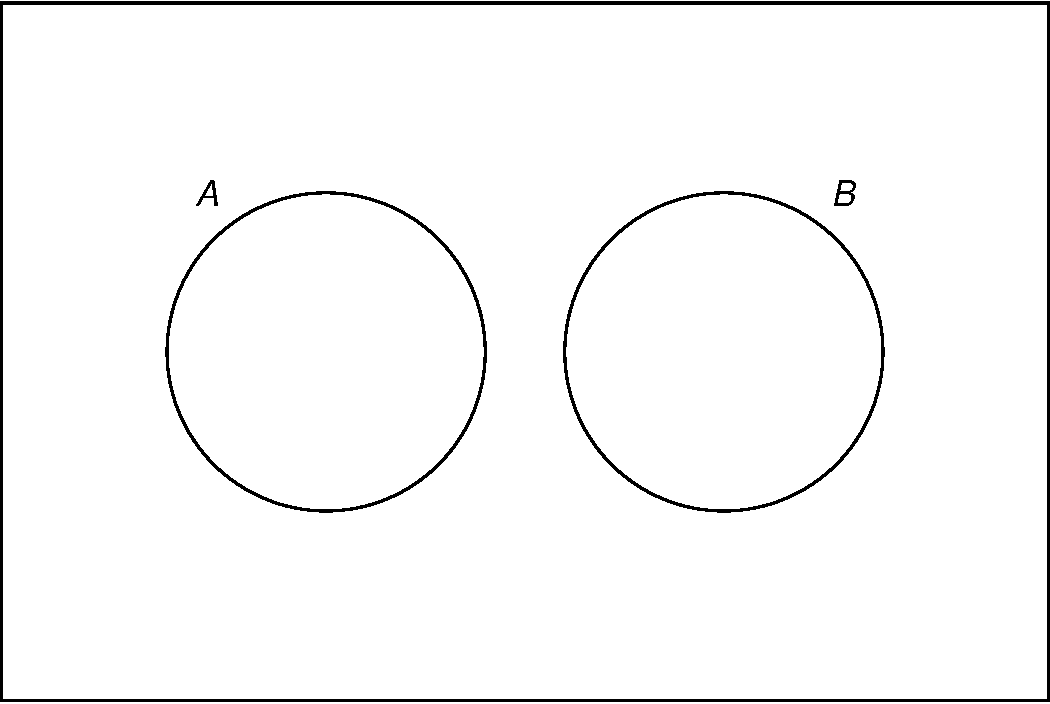
\includegraphics{_main_files/figure-latex/meprops-1} \caption[Mutually exclusive propositions]{Mutually exclusive propositions}\label{fig:meprops}
\end{marginfigure}

Each circle represents a proposition. You can think of it as surrounding
the possible situations where the proposition would be true. The circles
don't overlap because there is no possible situation where both
propositions in this example are true.

In contrast, these two propositions are not mutually exclusive:

\begin{itemize}
\tightlist
\item
  Confucius was born in Asia.
\item
  Confucius was born in the 6th Century B.C.
\end{itemize}

When propositons are not mutually exclusive, we say they are
\textbf{\emph{compatible}}. Compatible propositions overlap (Figure
\ref{fig:compropositions}). The region where the circles overlap
represents the possible scenarios where both propositions are true (the
``\(A \wedge B\) region'').

\begin{marginfigure}
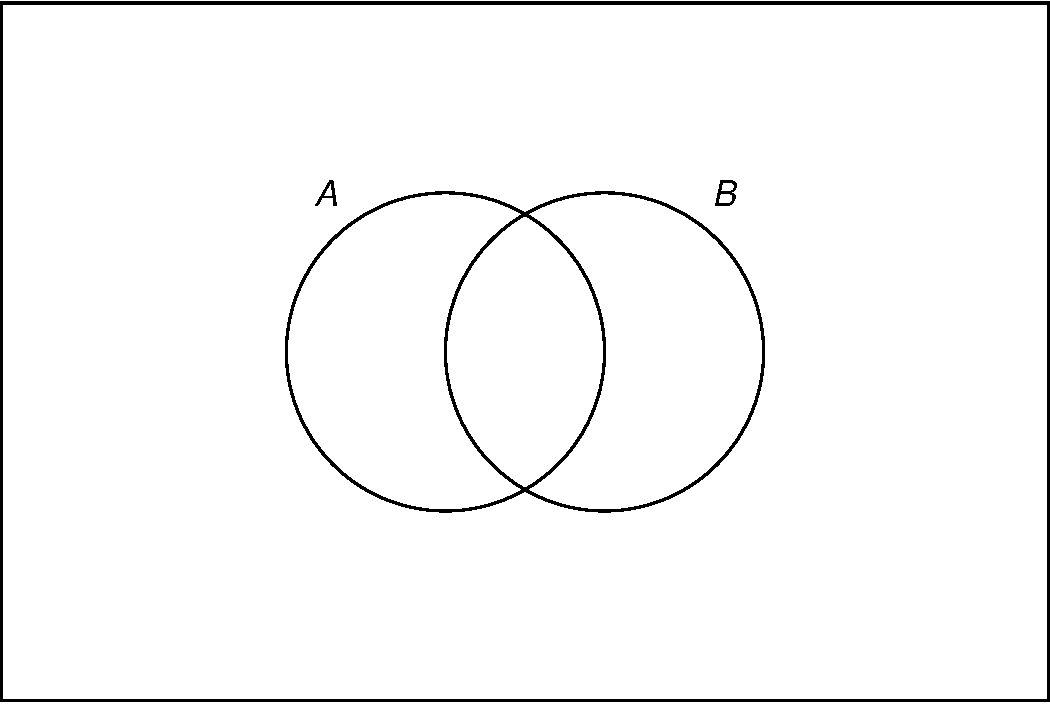
\includegraphics{_main_files/figure-latex/compropositions-1} \caption[Compatible propositions]{Compatible propositions}\label{fig:compropositions}
\end{marginfigure}

These are called \textbf{\emph{Euler diagrams}}, after the mathematician
Leonhard Euler (pronounced \emph{oiler}).\footnote{Leonhard Euler lived
  from \(1707\) to \(1783\). You may have encountered some of his work
  before if you've worked with logarithms or taken calculus.} You may
have seen Venn diagrams before, which are very similar. But in an Euler
diagram, the circles don't have to overlap.

\newthought{Sometimes} one circle will even contain another circle
entirely. Take this example:

\begin{itemize}
\tightlist
\item
  Confucius was born in Asia.
\item
  Confucius was born somewhere.
\end{itemize}

These propositions aren't just compatible. If the first is true, then
the second \emph{must} be true. Imagine an argument with the first
proposition as the premise and the second proposition as the conclusion.
The argument would be valid:

\begin{argument}
Confucius was born in Asia.\\
Therefore, Confucius was born.
\end{argument}

\begin{marginfigure}
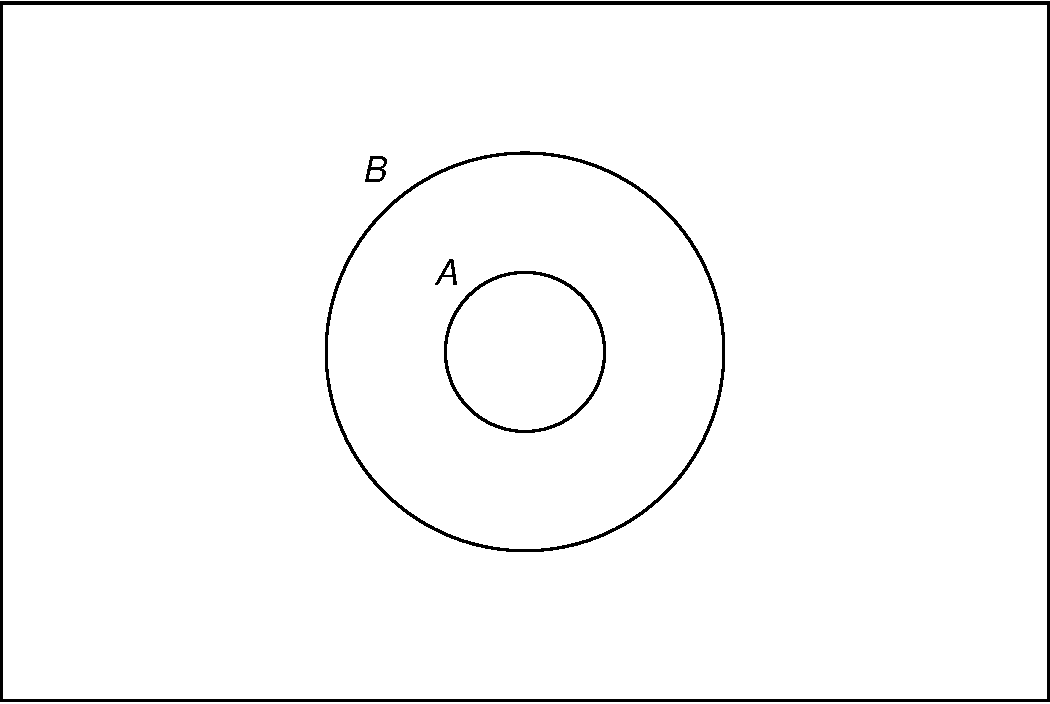
\includegraphics{_main_files/figure-latex/entailment-1} \caption[Logical entailment]{Logical entailment}\label{fig:entailment}
\end{marginfigure}

In this case we say that the first proposition \textbf{\emph{logically
entails}} the second. In terms of an Euler diagram, he first circle is
contained entirely in the second (Figure \ref{fig:entailment}). Because
there is no possible situation where the first proposition is true yet
the second false.

What if an argument has multiple premises? For example:

\begin{argument}
Zhuangzi was born in the Chinese province of Anhui.\\
Zhuoru was born in the Chinese city of Beijing.\\
Therefore, both Zhuangzi and Zhuoru were born in China.
\end{argument}

\begin{marginfigure}
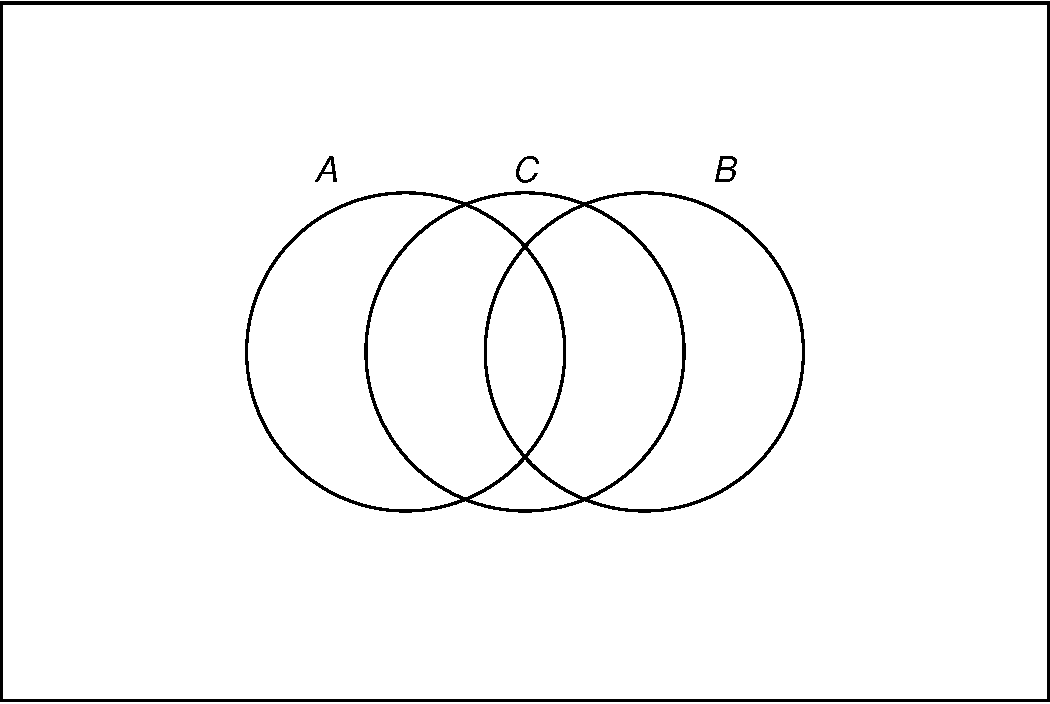
\includegraphics{_main_files/figure-latex/validtwopremises-1} \caption[A valid argument with two premises]{A valid argument with two premises}\label{fig:validtwopremises}
\end{marginfigure}

This argument is valid, and the diagram might look like Figure
\ref{fig:validtwopremises}. Notice how the \(A \wedge B\) region lies
entirely within the \(C\) circle. This reflects the argument's validity:
there is no way for the first two propositions to be true and the last
one false.

In contrast, an invalid argument would have a diagram like Figure
\ref{fig:invalidtwopremises}. This diagram allows for the possibility
that \(A\) and \(B\) are both true yet \(C\) is false; part of the
\(A \wedge B\) region falls outside the \(C\) circle.

\begin{marginfigure}
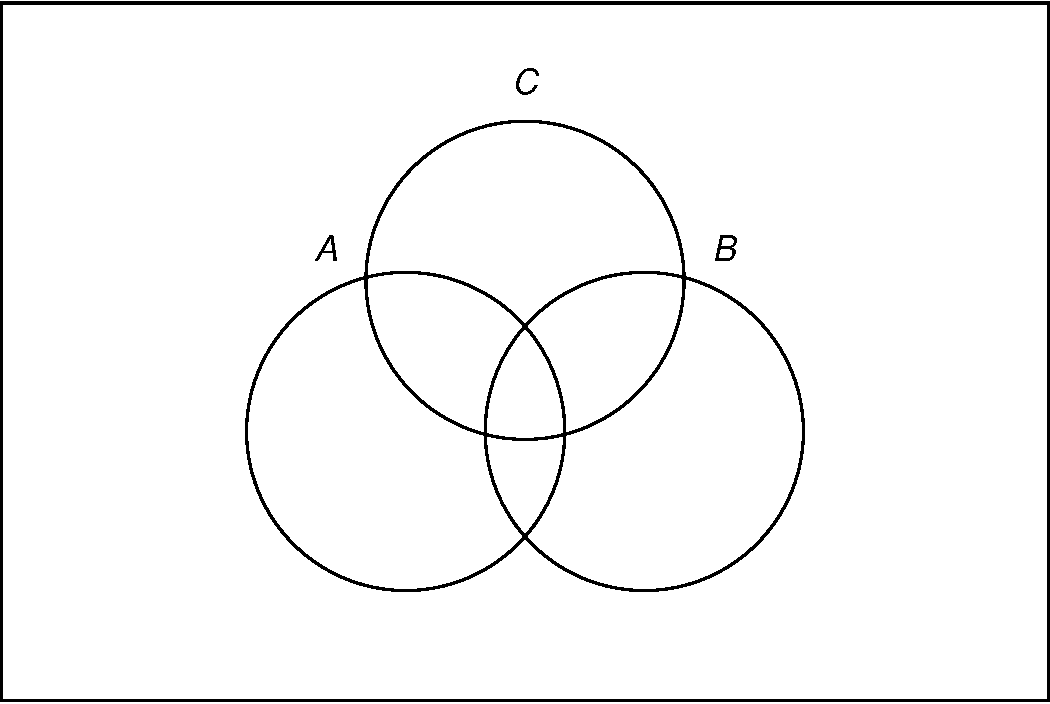
\includegraphics{_main_files/figure-latex/invalidtwopremises-1} \caption[An invalid argument with two premises]{An invalid argument with two premises}\label{fig:invalidtwopremises}
\end{marginfigure}

\hypertarget{strength}{%
\section{Strength}\label{strength}}

\newthought{Inductive} logic studies arguments that aren't necessarily
valid, but still ``strong''. A \textbf{\emph{strong}} argument is one
where the conclusion is highly probable, if the premises are true. For
example:

\begin{argument}
The sun has risen every day so far.\\
Therefore, the sun will rise again tomorrow.
\end{argument}

This argument isn't valid, because it's possible the conclusion is false
even though the premise is true. Maybe the sun will explode in the night
for some surprising reason. Or maybe the earth's rotation will be
stopped by alien forces.

These possibilities aren't very likely, of course. So the argument is
strong, even though it's not strictly valid. The premise gives us very
good reason to believe the conclusion, just not a 100\% guarantee.

In terms of an Euler diagram then, the premise circle isn't contained
entirely within the conclusion circle (Figure \ref{fig:strongarg}). We
have to leave some room for the possibility that the premise is true and
the conclusion false. But we can still convey that this possibility has
only a very slight chance of being true, by making it slim.

\begin{marginfigure}
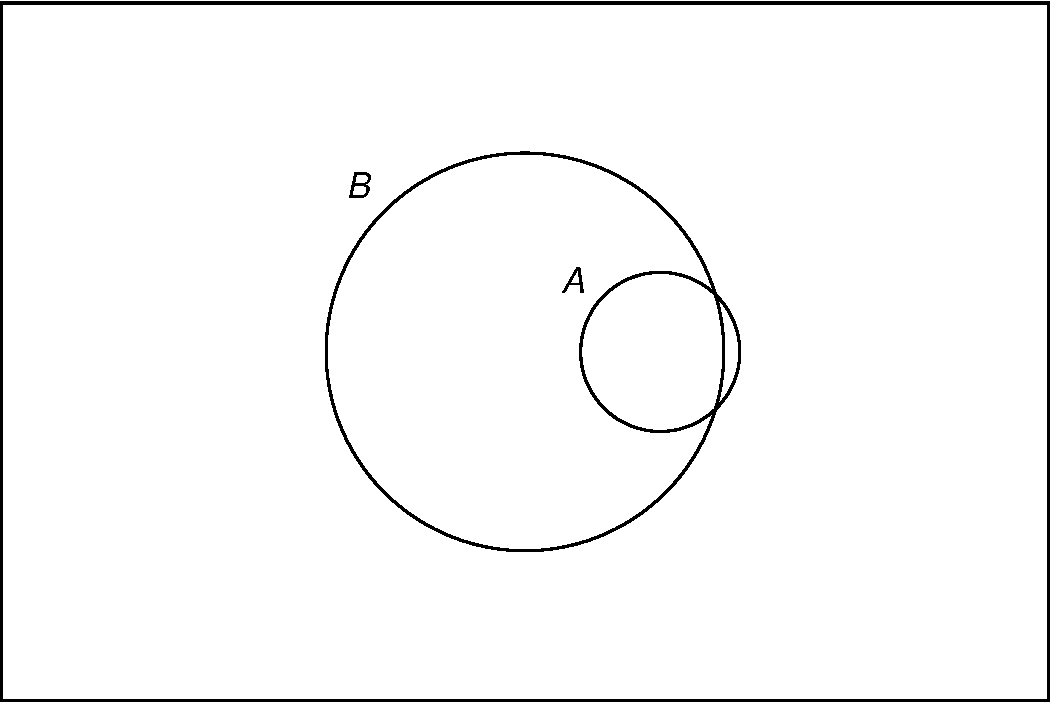
\includegraphics{_main_files/figure-latex/strongarg-1} \caption[A strong argument with premise $A$ and conclusion $B$]{A strong argument with premise $A$ and conclusion $B$}\label{fig:strongarg}
\end{marginfigure}






\begin{marginfigure}
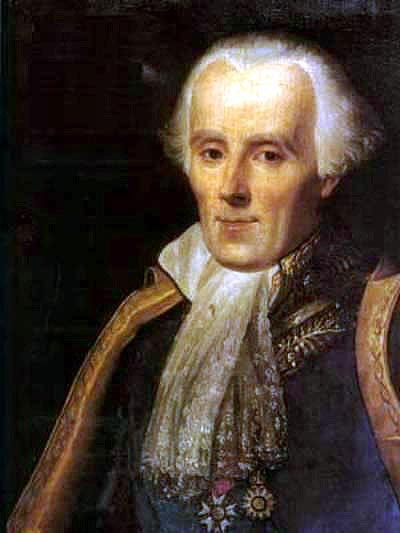
\includegraphics[width=1.33in]{img/laplace} \caption[Pierre Simone Laplace (1749--1827) developed
\href{https://bit.ly/2mU9WgW}{a formula} for calculating the probability
the sun will rise tomorrow. We'll learn how to do similar calculations
in the coming chapters.]{Pierre Simone Laplace (1749--1827) developed
\href{https://bit.ly/2mU9WgW}{a formula} for calculating the probability
the sun will rise tomorrow. We'll learn how to do similar calculations
in the coming chapters.}\label{fig:laplace}
\end{marginfigure}

We could also label the \emph{\(A\)-but-not-\(B\)} region with a small
number, if we knew exactly how unlikely this possibility was.

\newthought{Strength} comes in degrees. An argument's premises can make
the conclusion somewhat likely, very likely, almost certain, or
perfectly certain. So arguments range from weak, to somewhat strong, to
very strong, etc.

Strength differs from validity here, since validity is all-or-nothing.
If there is any possible way for the premises to be true and the
conclusion false, the argument is invalid---no matter how remote or
bizarre that possibility is.

Notice though, valid arguments are strong by definition. Since it's
impossible for a valid argument's conclusion to be false if the premises
are true, the premises make the conclusion 100\% probable. A valid
argument is the strongest possible argument.

\hypertarget{indargs}{%
\section{Forms of Inductive Argument}\label{indargs}}

\newthought{What} kinds of strong arguments are there, and how strong
are they? That's what the rest of this book is about, in a way. But we
can start by identifying some common forms of inductive argument right
now.

\newthought{Generalizing} from observed instances is one extremely
common form of argument:

\begin{argument}
Every raven I have every seen has been black.\\
Therefore, all ravens are black.
\end{argument}

Arguments of this kind are usually stronger the more instances you
observe. If you've only ever seen two ravens, this argument won't be
very compelling. But if you've seen thousands, then it's much stronger.

It also helps to observe different kinds of instances. If you've only
observed ravens in your city or town, then even the thousands you've
seen won't count for much. Maybe the raven population in your area is
unusual, and ravens on the other side of the world are all different
colours.

\newthought{Going} in the opposite direction, we can use what we know
about a general population to draw conclusions about particular
instances. We saw an example of this earlier:

\begin{argument}
Most birds can fly.\\
Tweety is a bird.\\
Therefore, Tweety can fly.
\end{argument}

Again, the strength of the inference depends on the details. If ``most
birds'' means \(99\%\), the argument is quite strong. If ``most'' only
means \(80\%\), then it's not so strong. (Usually ``most'' just means
more than \(50\%\).)

It also helps to know that Tweety is similar to the birds that can fly,
and different from the ones that can't. If we know that Tweety is small
and has feathers, that makes the argument stronger. If instead we know
that Tweety is large, and coloured black and white, that makes the
argument weaker. It suggests Tweety is a penguin.

\newthought{Inference} to the best explanation is another common form of
argument, quite different from the previous two. Here's an example:

\begin{argument}
My car won't start and the gas gauge reads `empty'.\\
Therefore, my car is out of gas.
\end{argument}

An empty tank would explain the sytmptoms described in the premise, so
the premise makes the conclusion plausible. There could be other
possible explanations, of course. Maybe the engine and the gas gauge
both just happened to break at the same time. But that would be quite a
coincidence, so this explanation isn't as good.

What makes one explanation better than another? That turns out to be a
very hard question, and there is no generally accepted answer. We'll
come back to this issue later, once we have a better grip on the basics
of probability.

\hypertarget{exercises-1}{%
\section*{Exercises}\label{exercises-1}}
\addcontentsline{toc}{section}{Exercises}

\begin{enumerate}
\item
  For each of the following arguments, say whether it is valid or
  invalid.

  \begin{enumerate}
  \def\labelenumii{\alph{enumii}.}
  \item
    \begin{argument}
    All cats have whiskers.\\
    Simba has whiskers.\\
    Therefore, Simba is a cat.
    \end{argument}
  \item
    \begin{argument}
    Ada Lovelace wrote the world's first computer program.\\
    Ada Lovelace was Lord Byron's daughter.\\
    Therefore, the first computer program was written by Lord Byron's
    daughter.
    \end{argument}
  \item
    \begin{argument}
    All Canadian residents are Russian citizens.\\
    Vladimir Putin is a Canadian resident.\\
    Therefore, Vladimir Putin is a Russian citizen.
    \end{argument}
  \item
    \begin{argument}
    Manitoba is located in either Saskatchewan, Ontario, or Quebec.\\
    Manitoba is not located in Saskatchewan.\\
    Manitoba is not located in Ontario.\\
    Therefore, Manitoba is located in Quebec.
    \end{argument}
  \item
    \begin{argument}
    If snow is black then pigs can fly.\\
    Snow is not black.\\
    Therefore, pigs cannot fly.
    \end{argument}
  \item
    \begin{argument}
    Either the moon is made of green cheese or pigs can fly.\\
    Pigs can't fly.\\
    Therefore the moon is made of green cheese.\\
    \end{argument}
  \end{enumerate}
\item
  For each pair of propositions, say whether they are mutually exclusive
  or compatible.

  \begin{enumerate}
  \def\labelenumii{\alph{enumii}.}
  \item
    Regarding the roll of an ordinary die:

    \begin{itemize}
    \tightlist
    \item
      The die will land on an even number.
    \item
      The die will land either \(4\) or \(5\).
    \end{itemize}
  \item
    Regarding the unemployment rate in your country tomorrow:

    \begin{itemize}
    \tightlist
    \item
      The unemployment rate will be at least \(5\%\).
    \item
      The unemployment rate will be exactly \(5\%\).
    \end{itemize}
  \item
    Regarding a party tomorrow:

    \begin{itemize}
    \tightlist
    \item
      Ani will be there and so will her sister PJ.
    \item
      PJ will not be there.
    \end{itemize}
  \end{enumerate}
\item
  True or false? If \(A\) and \(B\) are mutually exclusive, then \(A\)
  logically entails that \(B\) is false.
\item
  True or false? It is possible for \(A\) to logically entail \(B\) even
  though the reverse does not hold (i.e.~even though \(B\) does not
  logically entail \(A\)).
\item
  Create your own example of each of the three types of inductive
  argument described in this chapter:

  \begin{enumerate}
  \def\labelenumii{\alph{enumii}.}
  \tightlist
  \item
    Generalizing from Observed Instances
  \item
    Inferring an Instance from a Generalization
  \item
    Inference to the Best Explanation
  \end{enumerate}
\end{enumerate}

\hypertarget{truth-tables}{%
\chapter{Truth Tables}\label{truth-tables}}

\newthought{In} this chapter we'll introduce the last few concepts we
need from deductive logic, and we'll learn a useful technique in the
process: truth tables.

\hypertarget{connectives}{%
\section{Connectives}\label{connectives}}

\newthought{Complex} propositions can be built up out of other, simpler
propositions:

\begin{itemize}
\tightlist
\item
  Aegon is a tyrant \textbf{and} Brandon is a wizard.
\item
  \textbf{Either} Aegon is a tyrant \textbf{or} Brandon is a wizard.
\item
  \textbf{It's not true that} Aegon is a tyrant.
\end{itemize}

\begin{marginfigure}
Notice, we call \emph{it's not true that} a connective even though it
doesn't actually connect two propositions together.
\end{marginfigure}

Here we've used two simple propositions to build up longer, more complex
ones using the terms \emph{and}, \emph{either/or}, and \emph{it's not
true that}. Such terms are called \textbf{\emph{connectives}}.

The three connectives just listed are the only ones we'll need in this
book. Each has a name and a shorthand symbol:

\begin{longtable}[]{@{}llll@{}}
\toprule
Name & English & Symbol & Example\tabularnewline
\midrule
\endhead
conjunction & and & \(\wedge\) & \(A \wedge B\)\tabularnewline
disjunction & either/or & \(\vee\) & \(A \vee B\)\tabularnewline
negation & it's not true that & \(\neg\) & \(\neg A\)\tabularnewline
\bottomrule
\end{longtable}

Here are some more examples of complex propositions:

\begin{itemize}
\tightlist
\item
  \(F \wedge \neg G\): Florida is warm and Geneva is not.
\item
  \(\neg J \vee \neg K\): Either Jing won't come to the party or Kamal
  won't come.
\end{itemize}

\newthought{Sometimes} we also need parentheses, to avoid ambiguity.
Consider an example from arithmetic: \[ 4 \div 2 \times 2 = 1. \] Is
this equation true? That depends on what you mean. Does the division
operation come first, or the multiplication? So we use parentheses to
clarify: \(4 \div (2 \times 2) = 1\), but \((4 \div 2) \times 2 = 4\).

In logic we use parentheses to prevent ambiguity similarly. Consider:
\[ A \vee B \wedge C. \] This proposition is ambiguous, it has two
interpretations. In English we can distinguish them with a comma:

\begin{itemize}
\tightlist
\item
  Either Aegon is a tyrant or Brandon is a wizard, and Cerci is the
  queen.
\item
  Either Aegon is a tyrant, or Brandon is a wizard and Cerci is the
  queen.
\end{itemize}

Notice how these statements make different claims. The first takes a
definite stand on Cerci: she is the queen. It only leaves open the
question whether Aegon is a tyrant or Brandon is a wizard. Whereas the
second statement takes no definite stand on any of our three characters.
Maybe Aegon is a tyrant, maybe not. Maybe Brandon is a wizard and Cerci
is the queen, maybe not.

In logic we use parentheses to clarify which interpretation we mean:

\begin{itemize}
\tightlist
\item
  \((A \vee B) \wedge C\).
\item
  \(A \vee (B \wedge C)\).
\end{itemize}

Notice how the first statement is primarily an \(\wedge\) statement. It
uses \(\wedge\) to combine the simpler statements \(C\) and \(A \vee B\)
together. Whereas the second statement is primarily a \(\vee\)
statement. It uses \(\vee\) to combine \(A\) with \(B \wedge C\).

We call the last connective used to build up the statement the
\textbf{\emph{main connective}}.

\begin{itemize}
\tightlist
\item
  \((A \vee B) \wedge C\): main connective is \(\wedge\).
\item
  \(A \vee (B \wedge C)\): main connective is \(\vee\).
\end{itemize}

Two more examples:

\begin{itemize}
\tightlist
\item
  \(\neg (A \vee B)\): main connective is \(\neg\).
\item
  \(\neg A \vee B\): main connective is \(\vee\).
\end{itemize}

Technically, the last example should have parentheses to prevent
ambiguity, like so: \((\neg A) \vee B\). But things get cluttered and
hard to read if we add parentheses around every negation. So we have a
special understanding for \(\neg\) in order to keep things tidy.

\begin{marginfigure}
This special understanding for \(\mathbin{\sim}\) mirrors the one for
minus signs in arithmetic.
\end{marginfigure}

\begin{info}
The negation symbol \(\mathbin{\sim}\) only applies to the proposition
immediately following it.
\end{info}

So in the proposition \(\neg A \vee B\), the \(\neg\) only applies to
\(A\). And in \(\neg (A \wedge B) \vee C\), it only applies to
\(A \wedge B\).

\hypertarget{truth-tables-1}{%
\section{Truth Tables}\label{truth-tables-1}}

\newthought{The} truth of a complex proposition built using our three
connectives depends on the truth of its components. For example,
\(\neg A\) is false if \(A\) is true, and it's true if \(A\) is false:

\begin{longtable}[]{@{}cc@{}}
\caption{\label{tab:unnamed-chunk-28}Truth table for
\(\neg\)}\tabularnewline
\toprule
\(A\) & \(\neg A\)\tabularnewline
\midrule
\endfirsthead
\toprule
\(A\) & \(\neg A\)\tabularnewline
\midrule
\endhead
T & F\tabularnewline
F & T\tabularnewline
\bottomrule
\end{longtable}

Slightly more complicated is the rule for \(\&\):

\begin{longtable}[]{@{}ccc@{}}
\caption{\label{tab:unnamed-chunk-29}Truth table for
\(\wedge\)}\tabularnewline
\toprule
\(A\) & \(B\) & \(A \wedge B\)\tabularnewline
\midrule
\endfirsthead
\toprule
\(A\) & \(B\) & \(A \wedge B\)\tabularnewline
\midrule
\endhead
T & T & T\tabularnewline
T & F & F\tabularnewline
F & T & F\tabularnewline
F & F & F\tabularnewline
\bottomrule
\end{longtable}

There are four rows now because \(\&\) combines two propositions \(A\)
and \(B\) together to make the more complex proposition \(A \& B\).
Since each of those propositions could be either true or false, there
are \(2 \times 2 = 4\) possible situations to consider.

Notice that in only one of these situations is \(A \& B\) true, namely
the first row where both \(A\) and \(B\) are true.

The truth table for \(\vee\) (``either/or'') is a little more
surprising:

\begin{longtable}[]{@{}ccc@{}}
\caption{\label{tab:unnamed-chunk-30}Truth table for
\(\vee\)}\tabularnewline
\toprule
\(A\) & \(B\) & \(A \vee B\)\tabularnewline
\midrule
\endfirsthead
\toprule
\(A\) & \(B\) & \(A \vee B\)\tabularnewline
\midrule
\endhead
T & T & T\tabularnewline
T & F & T\tabularnewline
F & T & T\tabularnewline
F & F & F\tabularnewline
\bottomrule
\end{longtable}

Now the complex proposition is always true, except in one case: the last
row where \(A\) and \(B\) are both false. It makes sense that
\(A \vee B\) is false when both sides are false. But why is it true when
both sides are true? Doesn't ``Either \(A\) or \(B\)'' mean that
\emph{just one} of these is true?

Sometimes it does have that meaning. But sometimes it means ``Either A
or B, \emph{or both}''. Consider this exchange:

\begin{quote}
X: What are you doing tomorrow night?\\
Y: I'm either going to a friend's house or out to a club. I might even
do both, if there's time.
\end{quote}

Person Y isn't necessarily changing their mind here. They could just be
clarifying: they're doing at least one of these things, possibly even
both of them.

Although it's common to use ``either/or'' in English to mean \emph{just}
one or the other, in logic we use the more permissive reading. So
\(A \vee B\) means \emph{either \(A\), or \(B\), or both}.

We can always convey the stricter way of meaning ``either/or'' with a
more complex construction: \[(A \vee B) \wedge \neg (A \wedge B).\] That
says:
\[ \mbox{Either $A$ or $B$ is true, and it's not the case that both $A$ and $B$ are true}.\]
Which is just a very explicit way of saying: either one or the other,
but not both.

We can even verify that the complex construction captures the meaning we
want using a truth table. We start with an empty table, where the header
lists all the formulas we use to build up to the final, complex one
we're interested in:

\begin{longtable}[]{@{}cccccc@{}}
\toprule
\(A\) & \(B\) & \(A \vee B\) & \(A \& B\) & \(\neg(A \wedge B\)) &
\((A \vee B) \wedge \neg (A \wedge B)\)\tabularnewline
\midrule
\endhead
\(\;\) & & & & &\tabularnewline
\(\;\) & & & & &\tabularnewline
\(\;\) & & & & &\tabularnewline
\(\;\) & & & & &\tabularnewline
\bottomrule
\end{longtable}

Then we fill in the possible truth values for the simplest propositions,
\(A\) and \(B\):

\begin{longtable}[]{@{}cccccc@{}}
\toprule
\(A\) & \(B\) & \(A \vee B\) & \(A \& B\) & \(\neg(A \wedge B\)) &
\((A \vee B) \wedge \neg (A \wedge B)\)\tabularnewline
\midrule
\endhead
T & T & & & &\tabularnewline
T & F & & & &\tabularnewline
F & T & & & &\tabularnewline
F & F & & & &\tabularnewline
\bottomrule
\end{longtable}

Next we consult the truth tables above for \(\&\) and \(\vee\) to fill
in the columns at the next level of complexity:

\begin{longtable}[]{@{}cccccc@{}}
\toprule
\(A\) & \(B\) & \(A \vee B\) & \(A \& B\) & \(\neg(A \wedge B\)) &
\((A \vee B) \wedge \neg (A \wedge B)\)\tabularnewline
\midrule
\endhead
T & T & T & T & &\tabularnewline
T & F & T & F & &\tabularnewline
F & T & T & F & &\tabularnewline
F & F & F & F & &\tabularnewline
\bottomrule
\end{longtable}

Then move up to the next level of complexity. To fill in the column for
\(\neg(A \wedge B)\), we consult the column for \(A \wedge B\) and apply
the rules from the table for \(\neg\):

\begin{longtable}[]{@{}cccccc@{}}
\toprule
\(A\) & \(B\) & \(A \vee B\) & \(A \& B\) & \(\neg(A \wedge B\)) &
\((A \vee B) \wedge \neg (A \wedge B)\)\tabularnewline
\midrule
\endhead
T & T & T & T & F &\tabularnewline
T & F & T & F & T &\tabularnewline
F & T & T & F & T &\tabularnewline
F & F & F & F & T &\tabularnewline
\bottomrule
\end{longtable}

Finally, we consult the columns for \(A \vee B\) and
\(\neg(A \wedge B)\), and the table for \(\&\), to fill in the column
for \((A \vee B) \wedge \neg(A \& B)\):

\begin{longtable}[]{@{}cccccc@{}}
\toprule
\(A\) & \(B\) & \(A \vee B\) & \(A \& B\) & \(\neg(A \wedge B\)) &
\((A \vee B) \wedge \neg (A \wedge B)\)\tabularnewline
\midrule
\endhead
T & T & T & T & F & F\tabularnewline
T & F & T & F & T & T\tabularnewline
F & T & T & F & T & T\tabularnewline
F & F & F & F & T & F\tabularnewline
\bottomrule
\end{longtable}

Complex constructions like this are difficult at first, but don't worry.
With practice they quickly become routine.

\hypertarget{logical-truths-contradictions}{%
\section{Logical Truths \&
Contradictions}\label{logical-truths-contradictions}}

\newthought{Some} propositions come out true in every row of the truth
table. Consider \(A \vee \neg A\) for example:

\begin{longtable}[]{@{}ccc@{}}
\toprule
\(A\) & \(\neg A\) & \(A \vee \neg A\)\tabularnewline
\midrule
\endhead
T & F & T\tabularnewline
F & T & T\tabularnewline
\bottomrule
\end{longtable}

Such propositions are especially interesting because they \emph{must} be
true. Their truth is guaranteed, just as a matter of logic. So we call
them \textbf{\emph{logical truths}}.

The other side of this coin is propositions that are false in every row
of the truth table, like \(A \wedge \neg A\):

\begin{longtable}[]{@{}ccc@{}}
\toprule
\(A\) & \(\neg A\) & \(A \wedge \neg A\)\tabularnewline
\midrule
\endhead
T & F & F\tabularnewline
F & T & F\tabularnewline
\bottomrule
\end{longtable}

These propositions are called \textbf{\emph{contradictions}}.

Notice that the negation of a contradiction is a logical truth. For
example, consider the truth table for \(\neg (A \wedge \neg A)\):

\begin{longtable}[]{@{}cccc@{}}
\toprule
\(A\) & \(\neg A\) & \(A \wedge \neg A\) &
\(\neg (A \wedge \neg A)\)\tabularnewline
\midrule
\endhead
T & F & F & T\tabularnewline
F & T & F & T\tabularnewline
\bottomrule
\end{longtable}

\hypertarget{mutually-exclusivity-truth-tables}{%
\section{Mutually Exclusivity \& Truth
Tables}\label{mutually-exclusivity-truth-tables}}

\newthought{Truth} tables can be used to establish that two propositions
are mutually exclusive. A very simple example is the propositions \(A\)
and \(\neg A\):

\begin{longtable}[]{@{}cc@{}}
\toprule
\(A\) & \(\neg A\)\tabularnewline
\midrule
\endhead
T & F\tabularnewline
F & T\tabularnewline
\bottomrule
\end{longtable}

There is no row in the table where both propositions are true. And if
two propositions can't both be true, they are mutually exclusive by
definition.

A slightly more complex example is the propositions \(A \vee B\) and
\(\neg A \wedge \neg B\):

\begin{longtable}[]{@{}cccccc@{}}
\toprule
\(A\) & \(B\) & \(\neg A\) & \(\neg B\) & \(A \vee B\) &
\(\neg A \wedge \neg B\)\tabularnewline
\midrule
\endhead
T & T & F & F & T & F\tabularnewline
T & F & F & T & T & F\tabularnewline
F & T & T & F & T & F\tabularnewline
F & F & T & T & F & T\tabularnewline
\bottomrule
\end{longtable}

Again there's no row where \(A \vee B\) and \(\neg A \wedge \neg B\) are
both true. So they are mutually exclusive.

\hypertarget{entailment-equivalence}{%
\section{Entailment \& Equivalence}\label{entailment-equivalence}}

\newthought{Truth} tables can also be used to establish that an argument
is valid. Here's a very simple example:

\begin{quote}
\(A \wedge B\).\\
Therefore, \(A\).
\end{quote}

Obviously it's not possible for the premise to be true and the
conclusion false, so the argument is valid (if a bit silly).
Accordingly, there is no line of the truth table where \(A \wedge B\)
comes out true, yet \(A\) comes out false:

\begin{longtable}[]{@{}ccc@{}}
\toprule
\(A\) & \(B\) & \(A \wedge B\)\tabularnewline
\midrule
\endhead
T & T & T\tabularnewline
T & F & F\tabularnewline
F & T & F\tabularnewline
F & F & F\tabularnewline
\bottomrule
\end{longtable}

The only line where \(A \wedge B\) comes out true is the first one. And
on that line \(A\) is true too. So the argument from \(A \wedge B\) to
\(A\) is valid.

One more example:

\begin{quote}
\(A \vee B\).\\
\(\neg A\).\\
Therefore, \(B\).
\end{quote}

This argument is valid because the first premise says that at least one
of the two propositions \(A\) and \(B\) must be true, and the second
line says it's not \(A\). So it must be \(B\) that's true, as the
conclusion asserts. And once again there is no line of the truth table
where both \(A \vee B\) and \(\neg A\) are true, yet \(B\) is false:

\begin{longtable}[]{@{}cccc@{}}
\toprule
\(A\) & \(B\) & \(\neg A\) & \(A \vee B\)\tabularnewline
\midrule
\endhead
T & T & F & T\tabularnewline
T & F & F & T\tabularnewline
F & T & T & T\tabularnewline
F & F & T & F\tabularnewline
\bottomrule
\end{longtable}

The only line where both \(A \vee B\) and \(\neg A\) are true is the
third row, and \(B\) is true on that row. So once again the truth table
tells us this argument is valid.

In the \protect\hyperlink{visualizing-propositions}{previous chapter} we
introduced the concept of logical entailment. \(A\) logically entails
\(B\) when it's impossible for \(A\) to be true and \(B\) false. When
one proposition entails another, there is no line of the truth table
where the first proposition is true and the second is false.

\newthought{Sometimes} entailment goes in both directions: the first
proposition entails the second \emph{and the second entails the first}.
For example, not only does \(A \wedge B\) entail \(B \wedge A\), but
also \(B \wedge A\) entails \(A \wedge B\).

We say such propositions are \textbf{\emph{logically equivalent}}. In
terms of truth tables, their columns match perfectly, they are identical
copies of T's and F's.

\begin{longtable}[]{@{}cccc@{}}
\toprule
\(A\) & \(B\) & \(A \wedge B\) & \(B \wedge A\)\tabularnewline
\midrule
\endhead
T & T & T & T\tabularnewline
T & F & F & F\tabularnewline
F & T & F & F\tabularnewline
F & F & F & F\tabularnewline
\bottomrule
\end{longtable}

A more complex example is the propositions \(\neg (A \vee B)\) and
\(\neg A \wedge \neg B\):

\begin{longtable}[]{@{}ccccccc@{}}
\toprule
\(A\) & \(B\) & \(\neg A\) & \(\neg B\) & \(A \vee B\) &
\(\neg(A \vee B)\) & \(\neg A \wedge \neg B\)\tabularnewline
\midrule
\endhead
T & T & F & F & T & F & F\tabularnewline
T & F & F & T & T & F & F\tabularnewline
F & T & T & F & T & F & F\tabularnewline
F & F & T & T & F & T & T\tabularnewline
\bottomrule
\end{longtable}

Here again the columns under these two propositions are identical.

\hypertarget{summary}{%
\section{Summary}\label{summary}}

\newthought{Connectives} can be used to build more complex propositions,
like \(A \wedge B\) or \(A \vee \neg B\). We introduced three
connectives:

\begin{itemize}
\tightlist
\item
  \(\neg A\) means it's not true that \(A\).
\item
  \(A \wedge B\) means both \(A\) and \(B\) are true.
\item
  \(A \vee B\) means either \(A\) is true, or \(B\) is true, \emph{or
  both are true}.
\end{itemize}

In a complex proposition, the main connective is the last one used to
build it up from simpler components. In \(A \vee \neg B\) the main
connective is the \(\vee\).

An argument's validity can be established with a truth table, if there's
no row where all the premises have a T and yet the conclusion has an F.

Truth tables can also be used to establish that two propositions are
mutually exclusive, if there is no row of the table where both
propositions have a T.

Logically equivalent propositions entail one another. When two
propositions have identical columns in a truth table, they are logically
equivalent.

\hypertarget{exercises-2}{%
\section*{Exercises}\label{exercises-2}}
\addcontentsline{toc}{section}{Exercises}

\begin{enumerate}
\item
  Using the following abbreviations:

  \[
    \begin{aligned}
       A &= \mbox{Asha loves Cerci},\\
       B &= \mbox{Balon loves Cerci},
    \end{aligned}
  \]

  translate each of the following into logicese (e.g.
  \(\neg A \vee B\)).

  \begin{enumerate}
  \def\labelenumii{\alph{enumii}.}
  \tightlist
  \item
    Asha doesn't love Cerci.
  \item
    Asha loves Cerci and Balon loves Cerci.
  \item
    Asha loves Cerci but Balon does not.
  \item
    Neither Asha nor Balon loves Cerci.
  \end{enumerate}
\item
  For each pair of propositions, use a truth table to determine whether
  they are mutually exclusive.

  \begin{enumerate}
  \def\labelenumii{\alph{enumii}.}
  \tightlist
  \item
    \(A \wedge B\) and \(A \wedge \neg B\).
  \item
    \(A\) and \(\neg B\).
  \item
    \(A \vee \neg A\) and \(A \wedge \neg A\).
  \end{enumerate}
\item
  For each pair of propositions, use a truth table to determine whether
  they are logically equivalent.

  \begin{enumerate}
  \def\labelenumii{\alph{enumii}.}
  \tightlist
  \item
    \(\neg A \vee B\) and \(\neg (A \wedge \neg B)\).
  \item
    \(A\) and \((A \wedge B) \vee (A \wedge \neg B)\).
  \item
    \(A\) and \((B \wedge A) \vee (B \wedge \neg A)\).
  \end{enumerate}
\item
  The proposition \(A \vee (B \wedge C)\) features three simple
  propositions, so its truth table has 8 rows. Fill in the rest of the
  table:

  \begin{longtable}[]{@{}ccccc@{}}
  \toprule
  \(A\) & \(B\) & \(C\) & \(B \wedge C\) &
  \(A \vee (B \wedge C)\)\tabularnewline
  \midrule
  \endhead
  T & T & T & &\tabularnewline
  T & T & F & &\tabularnewline
  T & F & T & &\tabularnewline
  T & F & F & &\tabularnewline
  F & T & T & &\tabularnewline
  F & T & F & &\tabularnewline
  F & F & T & &\tabularnewline
  F & F & F & &\tabularnewline
  \bottomrule
  \end{longtable}
\item
  Use a truth table to determine whether the propositions
  \(A \vee (B \wedge C)\) and \((A \vee B) \wedge (A \vee C)\) are
  equivalent.
\end{enumerate}

\hypertarget{the-gamblers-fallacy}{%
\chapter{The Gambler's Fallacy}\label{the-gamblers-fallacy}}

\begin{epigraph}
Applied statistics is hard.\\
---Andrew Gelman
\end{epigraph}

\newthought{My} wife's family keeps having girls. My wife has two
sisters and she and her sisters each have two daughters, with no other
siblings or children. That's nine girls in a row!

\begin{marginfigure}
Note that girl and boy aren't the only two possibilities. The next child
could also be intersex.

Boy and girl are the likely alternatives, since fewer than \(2\%\) of
children born are intersex. (The exact percentage is unclear because the
exact definition of ``interesex'' is controversial.)

But many intersex children have undergone risky or painful surgeries and
treatments, sometimes without ever being told. So it's important to
recognize intersex as a third category.

Fashion model
\href{https://en.wikipedia.org/wiki/Hanne_Gaby_Odiele}{Hanne Gaby
Odiele} is one example of a famous intersex person. She learned she was
intersex just weeks before starting her modeling career.
\end{marginfigure}

So are they due for a boy next? Here are three possible answers.

\emph{Answer 1.} Yes, the next baby is more likely to be a boy. Ten
girls in a row would be a \emph{really} unlikely outcome.

\emph{Answer 2.} No, the next baby is actually more likely to be a girl.
Girls run in the family! Something about this family clearly predispose
them to have girls.

\emph{Answer 3.} No, the next baby is equally likely to be a boy
vs.~girl. Each baby's sex is determined by a purely random event,
similar to a coin flip. So it's equal odds every time. The nine girls so
far is just a coincidence.

Which answer is correct?

\hypertarget{independence}{%
\section{Independence}\label{independence}}

\newthought{It} all hangs on whether the sex of each baby is
``independent'' of the others. Two events are
\textbf{\emph{independent}} when the outcome of one doesn't change the
probability of the other.

A clear example of independence is \textbf{\emph{sampling with
replacement}}. Suppose we have an urn with \(50\) black marbles and
\(50\) white ones. You draw a ball at random, then put it back. Then you
give the urn a good hard shake and draw at random again. The two draws
are independent in this case. Each time you draw, the number of black
vs.~white marbles is the same, and they're all randomly mixed up.

Even if you were to draw ten white balls in a row, the eleventh draw
would still be a \(50\)-\(50\) shot! It would just be a coincidence that
you drew ten white balls in a row. Because there's always an even mix of
black and white marbles, and you're always picking one at random.

But now imagine sampling \textbf{\emph{without replacement}}. The
situation is the same, except now you set aside each ball you draw
rather than put it back. Now the draws are \textbf{\emph{dependent}}. If
you draw a black ball on the first draw, the odds of black on the next
draw go down. There are only \(49\) black balls in the urn now, vs.
\(50\) white.

\hypertarget{fairness}{%
\section{Fairness}\label{fairness}}

\newthought{Flips} of an ordinary coin are also independent. Even if you
get ten heads in a row, the eleventh toss is still \(50\)-\(50\). If
it's \emph{really} an ordinary coin, the ten heads in a row was just a
coincidence.

Coin flips aren't just independent, they're also \emph{unbiased}: heads
and tails are equally likely. A process is \textbf{\emph{biased}} if
some outcomes are more likely than others. For example, a loaded coin
that comes up heads \(3/4\) of the time is biased.

So coin flips are unbiased \emph{and} independent. We call such
processes \textbf{\emph{fair}}.
\[ \mbox{Fair = Unbiased + Independent}.\] Another example of a fair
process is drawing from our black/white urn with replacement. There are
\(50\) black and \(50\) white marbles on every draw, so black and white
have equal probability every time.

But drawing without replacement is not a fair process, because the draws
are not independent. Removing a black ball makes the chance of black on
the next draw go down.

\hypertarget{the-gamblers-fallacy-1}{%
\section{The Gambler's Fallacy}\label{the-gamblers-fallacy-1}}

\newthought{Gambling} often involves fair processes: fair dice, fair
roulette wheels, fair decks of cards, etc. But people sometimes forget
that fair processes are independent. If a roulette wheel comes up black
nine times in a row, they figure it's ``due'' for red. Or if they get a
bunch of bad hands in a row at poker, they figure they're due for a good
one soon.

This way of thinking is called \emph{the gambler's fallacy}. A fallacy
is a mistake in reasoning. The mistake here is failing to fully account
for independence. These gamblers know the process in question is fair,
in fact that's a key part of their reasoning. They know it's unlikely
that the roulette wheel will land on black ten times in a row because a
fair wheel should land on black and red equally often. But then they
overlook the fact that fair also means independent, and independent
means the last nine spins tell us nothing about the tenth spin.

The gambler's fallacy is so seductive that it can be hard to find your
way out of it. Here's one way to think about it that may help. Imagine
the gambler's point of view at two different times: before the ten spins
of the wheel, and after. Before, the gambler is contemplaing the
likelihood of getting ten black spins in a row:

\[  \_ \, \_ \,\_ \,\_ \,\_ \,\_ \,\_ \,\_ \,\_ \,\_ \, ? \]

From that vantage point, the gambler is exactly right to think it's
unlikely these ten spins will all land on black. But now imagine their
point of view after observing (to their surprise) the first nine spins
all landing black:

\[ B \, B \, B \, B \, B \, B \, B \, B \, B  \, \_ \,? \]

Now how likely is it these ten spins will all land black? Well, just one
more spin has to land black now to fulfill this unlikely prophecy. So
it's not such a long shot anymore. In fact it's a \(50\)-\(50\) shot.
Although it was very unlikely the first nine spins would turn out this
way, now that they have, it's perfectly possible the tenth will turn out
the same.

\hypertarget{ignorance-is-not-a-fallacy}{%
\section{Ignorance Is Not a Fallacy}\label{ignorance-is-not-a-fallacy}}

\newthought{At} this point you may have a nagging thought at the back of
your mind. If we flipped a coin 100 times and it landed heads every
time, wouldn't we conclude the next toss will probably land heads? How
could that be a mistake?!

The answer: it's not a fallacy. It \emph{would} be a fallacy if you knew
the coin was fair. But if you didn't know that for sure, then landing
100 heads in a row would be enough to convince you it's not fair.

The gambler's fallacy only occurs when you know a process is fair, and
then you fail to reason accordingly. If you don't know whether a process
is fair, then you aren't making a logical error by reasoning according
to a different assumption.

So, is the gambler's fallacy at work if my wife's family expects a boy
next? As it turns out,
\href{https://stat.duke.edu/~dalene/chance/chanceweb/144.rodgers.pdf}{the
process that determines the sex of a child is pretty much
fair}.\footnote{The question isn't completely settled though, as far as
  I could tell from my (not very thorough) research.} So the correct
answer to our opening question was Answer 3.

Most people don't know about the relevant research, though. They may
(like me) only know a bit from high school biology about how sex is
usually determined at conception. But it's still possible for all they
know that some people's eggs are more likely to select sperm cells with
an X chromosome, for example.

So it's not necessarily a fallacy if my in-laws expect a boy next. It
could just be a reasonable conclusion given the information available. A
fallacy is an error in reasoning, not a lack of knowledge.

\hypertarget{the-hot-hand-fallacy}{%
\section{The Hot Hand Fallacy}\label{the-hot-hand-fallacy}}

\newthought{Sometimes} a basketball player hits a lot of baskets in a
row and people figure they're on fire: they've got a ``hot hand''. But
\href{http://www.sciencedirect.com/science/article/pii/0010028585900106?via\%3Dihub}{a
famous study published in 1985} found that these streaks are just a
coincidence. Each shot is still independent of the others. Is the hot
hand an example of the gambler's fallacy?

Most people don't know about the famous 1985 study. Certainly nobody
knew what the result of the study would be before it was conducted. So a
lot of believers in the hot hand were in the unfortunate position of
just not knowing a player's shots are independent. So the hot hand isn't
the same as the gambler's fallacy.

Believers in the hot hand may be guilty of a different fallacy, though.
That same study analyzed the reasoning that leads people to think a
player's shots are dependent. Their conclusion: people tend to see
patterns in sequences of misses and hits even when they're random. So
there may be a second, different fallacy at work, the ``hot hand
fallacy''.

Things might actually be even more complicated than that, though.
\href{https://www.gsb.stanford.edu/insights/jeffrey-zwiebel-why-hot-hand-may-be-real-after-all}{Some
recent studies} found that the hot hand may actually be real after all!
How could that be possible? What did the earlier studies miss?

It's still being researched, but one possibility is: defense. When a
basketball player gets in the zone, the other team ups their defense.
The hot player has to take harder shots. So one of the recent studies
added a correction to account for increased difficulty. And another
looked at baseball instead, where they did find evidence of streaks.

\begin{marginfigure}
But here's \href{https://www.youtube.com/watch?v=WStmFKp1x3g}{Selena
Gomez and Nobel prize winner Richard Thaler} telling a bit of the story
in a clip from the 2015 movie \emph{The Big Short}.
\end{marginfigure}

The full story of the hot hand fallacy has yet to be told it seems.

\hypertarget{exercises-3}{%
\section*{Exercises}\label{exercises-3}}
\addcontentsline{toc}{section}{Exercises}

\begin{enumerate}
\item
  Suppose you are going to draw a card at random from a standard deck.
  For each pair of propositions, say whether they are independent or
  not.

  \begin{enumerate}
  \def\labelenumii{\alph{enumii}.}
  \item
    \(A\): the card is red.\\
    \(B\): the card is an ace.
  \item
    \(A\): the card is red.\\
    \(B\): the card is a diamond.
  \item
    \(A\): the card is an ace.\\
    \(B\): the card is a spade.
  \item
    \(A\): the card is a Queen.\\
    \(B\): the card is a face card.
  \end{enumerate}
\item
  After one draw with replacement, drawing a second marble from an urn
  filled with \(50\) black and \(50\) white marbles is a \_\_\_\_\_\_
  process.

  \begin{enumerate}
  \def\labelenumii{\alph{enumii}.}
  \tightlist
  \item
    Independent
  \item
    Fair
  \item
    Unbiased
  \item
    All of the above
  \item
    None of the above
  \end{enumerate}
\item
  After one draw \emph{without} replacement, drawing a second marble
  from an urn filled with \(50\) black and \(50\) white marbles is a
  \_\_\_\_\_\_ process.

  \begin{enumerate}
  \def\labelenumii{\alph{enumii}.}
  \tightlist
  \item
    Independent
  \item
    Fair
  \item
    Unbiased
  \item
    All of the above
  \item
    None of the above
  \end{enumerate}
\item
  For each of the following examples, say whether it is an instance of
  the gambler's fallacy.

  \begin{enumerate}
  \def\labelenumii{\alph{enumii}.}
  \item
    You're playing cards with your friends using a standard, randomly
    shuffled deck of \(52\) cards. You're about half-way through the
    deck and no aces have been drawn yet. You conclude that an ace is
    due soon, and thus the probability the next card is an ace has gone
    up.
  \item
    You're holding a six-sided die, which you know to be fair. You're
    going to roll it \(60\) times. You figure about \(10\) of those
    rolls should be threes. But after \(59\) rolls, you've rolled a
    three only five times. You figure that the probability of a three on
    the last roll has gone up: it's higher than just \(1/6\).
  \item
    You know the lottery numbers in Ontario are selected using a fair
    process. So it's really unlikely that someone will win two weeks in
    a row. Your friend won last week, so you conclude their chances of
    winning this week too are even lower than usual.
  \item
    You're visiting a new country where corruption is common, so you
    aren't sure whether the lottery there is fair. You see on the news
    that the King's cousin won the lottery two weeks in a row. You
    conclude that their chances of winning next week are higher than
    normal, because the lottery is rigged in their favour.
  \end{enumerate}
\end{enumerate}

\hypertarget{calculating-probabilities}{%
\chapter{Calculating Probabilities}\label{calculating-probabilities}}

\newthought{Imagine} you're going to flip a fair coin twice. You could
get two heads, two tails, or one of each. How probable is each outcome?

It's tempting to say they're equally probable, \(1/3\) each. But
actually the first two are only \(1/4\) likely, while the last is
\(1/2\) likely. Why?

There are actually four possible outcomes here, but we have to consider
the order of events to see how. If you get one each of heads and tails,
what order will they come in? You could get the head first and then the
tail, or the reverse.

So there are four possible sequences: HH, TT, HT, and TH. And all four
sequences are equally likely, a probability of \(1/4\).

How do we know each sequence has \(1/4\) probability though? And how
does that tell us the probability is \(1/2\) that you'll get one each of
heads and tails? We need to introduce some mechanics of probability to
settle these questions.

\hypertarget{multiplying-probabilities}{%
\section{Multiplying Probabilities}\label{multiplying-probabilities}}

\newthought{We} denote the probability of proposition \(A\) with
\(Pr(A)\). For example, \(Pr(A)=2/3\) means there's a \(2/3\) chance
\(A\) is true.

Now, our coin is fair, and by definition that means it always has a
\(1/2\) chance of landing heads and a \(1/2\) chance of landing tails.
For a single toss, we can use \(H\) for the proposition that it lands
heads, and \(T\) for the proposition that it lands tails. We can then
write \(Pr(H) = 1/2\) and \(Pr(T) = 1/2\).

For a sequence of two tosses, we can use \(H_1\) for heads on the first
toss, and \(H_2\) for heads on the second toss. Similarly, \(T_1\) and
\(T_2\) represent tails on the first and second tosses, respectively.
The four possible sequences are then expressed by the complex
propositions:

\begin{itemize}
\tightlist
\item
  \(H_1 \,\&\, H_2\),
\item
  \(T_1 \,\&\, T_2\),
\item
  \(H_1 \,\&\, T_2\),
\item
  \(T_1 \,\&\, H_2\).
\end{itemize}

We want to calculate the probabilities of these propositions. For
example, we want to know what number \(Pr(H_1 \,\&\, H_2)\) is equal to.

Because the coin is fair, we know \(Pr(H_1) = 1/2\) and
\(Pr(H_2) = 1/2\). The probability of heads on any given toss is always
\(1/2\), no matter what came before. To get the probability of
\(H_1 \,\&\, H_2\) it's then natural to compute: \[
  \begin{aligned}
    Pr(H_1 \,\&\, H_2) &= Pr(H_1) \times Pr(H_2)\\
                       &= 1/2 \times 1/2\\
                       &= 1/4.
  \end{aligned}
\] And this is indeed correct, but \emph{only because the coin is fair
and thus the tosses are independent}. The following is a general rule of
probability:

\begin{description}
\item[The Multiplication Rule]
If \(A\) and \(B\) are independent, then
\(Pr(A \,\&\, B) = Pr(A) \times Pr(B)\).
\end{description}

So, because our two coin tosses are independent, we can multiply to
calculate \(Pr(H_1 \,\&\, H_2) = 1/4\). And the same reasoning applies
to all four possible sequences, so we have: \[
  \begin{aligned}
    Pr(H_1 \,\&\, H_2) &= 1/4,\\
    Pr(T_1 \,\&\, T_2) &= 1/4,\\
    Pr(H_1 \,\&\, T_2) &= 1/4,\\
    Pr(T_1 \,\&\, H_2) &= 1/4.
  \end{aligned}
\]

\newthought{The} Multiplication rule only applies to independent
propositions. Otherwise it gives the wrong answer.

For example, the propositions \(H_1\) and \(T_1\) are definitely not
independent. If the coin lands heads on the first toss (\(H_1\)), that
drastically alters the chances of tails on the first toss (\(T_1\)). It
changes that probability to zero! If you were to apply the
Multiplication Rule though, you would get
\(Pr(H_1 \,\&\, T_1) = Pr(H_1) \times Pr(T_1) = 1/2 \times 1/2 = 1/4\),
which is definitely wrong.

\begin{warning}
Only use the Multiplication Rule on independent propositions.
\end{warning}

\hypertarget{adding-probabilities}{%
\section{Adding Probabilities}\label{adding-probabilities}}

\newthought{We} observed that you can get one head and one tail two
different ways. You can either get heads then tails
(\(H_1 \,\&\, T_2\)), or you can get tails then heads
(\(T_1 \,\&\, H_2\)). So the logical expression for ``one of each'' is:

\[ (H_1 \,\&\, T_2) \vee (T_1 \,\&\, H_2). \]

This proposition is a disjunction: its main connective is \(\vee\). How
do we calculate the probability of a disjunction?

\begin{description}
\item[The Addition Rule]
If \(A\) and \(B\) are mutually exclusive, then
\(Pr(A \vee B) = Pr(A) + Pr(B)\).
\end{description}

In this case the two sides of our disjunction are mutually exclusive.
They describe opposite orders of affairs. So we can apply the Addition
Rule to calculate:

\[
  \begin{aligned}
    Pr((H_1 \,\&\, T_2) \vee (T_1 \,\&\, H_2)) 
      &= Pr(H_1 \,\&\, T_2) + Pr(T_1 \,\&\, H_2)\\
      &= 1/4 + 1/4\\
      &= 1/2.
  \end{aligned}      
\]

\newthought{This} completes the solution to our opening problem. We've
now computed the three probabilities we wanted:

\begin{itemize}
\tightlist
\item
  \(Pr(\mbox{2 heads}) = Pr(H_1 \,\&\, H_2) = 1/2 \times 1/2 = 1/4\),
\item
  \(Pr(\mbox{2 tails}) = Pr(T_1 \,\&\, T_2) = 1/2 \times 1/2 = 1/4\),
\item
  \(Pr(\mbox{One of each}) = Pr((H_1 \,\&\, T_2) \vee (T_1 \,\&\, H_2)) = 1/4 + 1/4 = 1/2\).
\end{itemize}

In the process we introduced two central rules of probability, one for
\(\,\&\,\) and one for \(\vee\). The multiplication rule for \(\,\&\,\)
only applies when the propositions are independent. The addition rule
for \(\,\vee\,\) only applies when the propositions are mutually
exclusive.

\newthought{Why} does the addition rule for \(\vee\) sentences only
apply when the propositions are mutually exclusive? Well imagine the
weather forecast says there's a \(90\%\) chance of rain in the morning,
and there's also a \(90\%\) chance of rain in the afternoon. What's the
chance it'll rain at some point during the day, either in the morning or
the afternoon? If we calculate \(Pr(M \vee A) = Pr(M) + Pr(A)\), we get
\(90\% + 90\% = 180\%\), which doesn't make any sense. There can't be a
\(180\%\) chance of rain tomorrow.

The problem is that \(M\) and \(A\) are not mutually exclusive. It could
rain all day, both morning and afternoon. We'll see the correct way to
handle this kind of situation in
\protect\hyperlink{calculating-probabilities-part-ii}{Chapter 7}. In the
meantime just be careful:

\begin{warning}
Only use the Addition Rule on mutually exclusive propositions.
\end{warning}

\hypertarget{exclusivity-vs.independence}{%
\section{Exclusivity
vs.~Independence}\label{exclusivity-vs.independence}}

\begin{marginfigure}
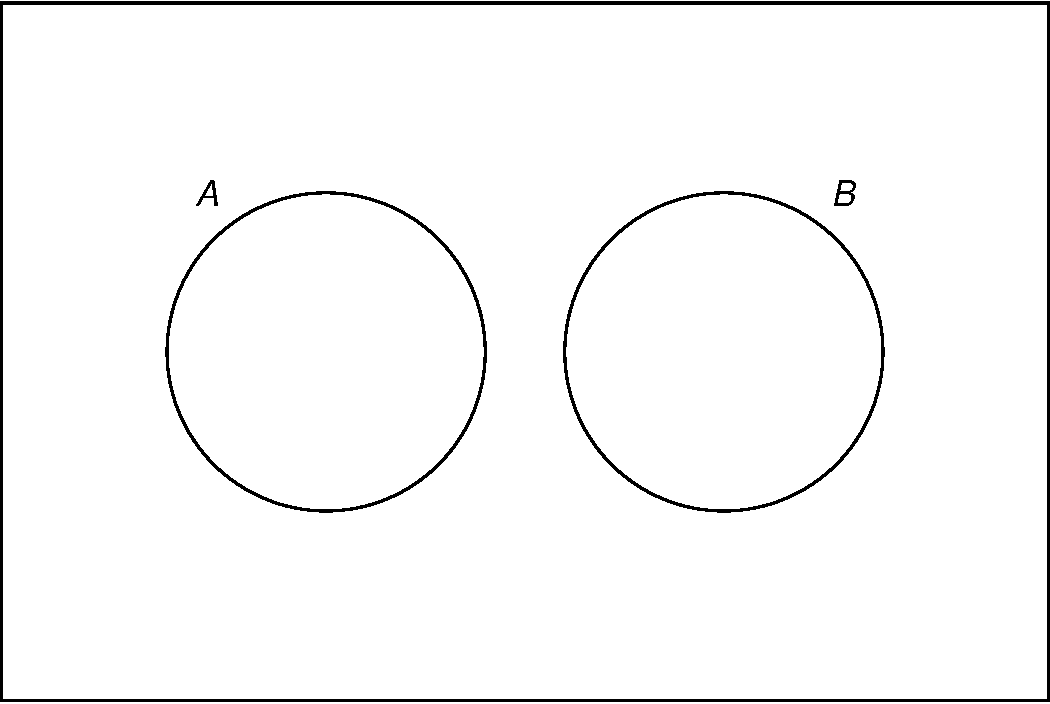
\includegraphics{_main_files/figure-latex/unnamed-chunk-53-1} \caption[Mutually exclusive propositions don't overlap]{Mutually exclusive propositions don't overlap}\label{fig:unnamed-chunk-53}
\end{marginfigure}

\newthought{Exclusivity} and independence can be hard to keep straight
at first. One way to keep track of the difference is to remember that
mutually exclusive propositions don't overlap, but independent
propositions usually do. Independence means the truth of one proposition
doesn't affect the chances of the other. So if you find out that \(A\)
is true, \(B\) still has the same chance of being true. Which means
there have to be some \(B\) possibilities within the \(A\) circle
(unless the probability of \(A\) was zero to start with).

\begin{marginfigure}
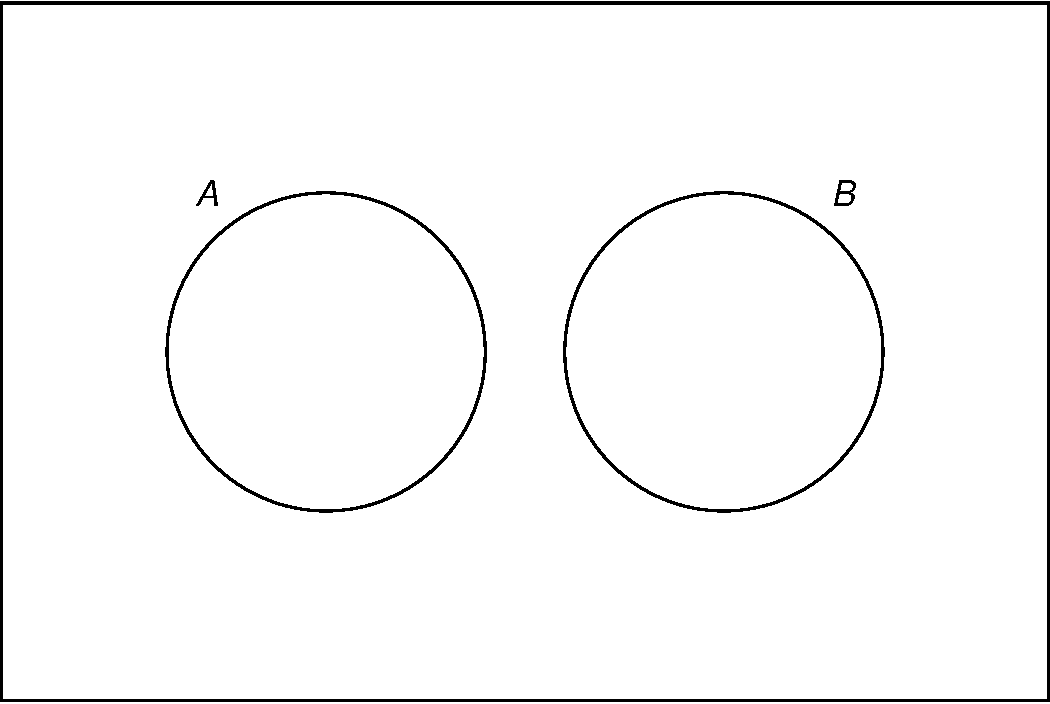
\includegraphics{_main_files/figure-latex/unnamed-chunk-54-1} \caption[Independent propositions do overlap (unless one of them has zero probability)]{Independent propositions do overlap (unless one of them has zero probability).}\label{fig:unnamed-chunk-54}
\end{marginfigure}

So independence and exclusivity are very different. Generally speaking,
exclusive propositions are not independent, and independent propositions
are not exclusive.

There is one exception. If \(\p(A) = 0\), then \(A\) and \(B\) can be
both independent and mutually exclusive. If they're mutually exclusive,
the probability of \(A\) just stays \(0\) after \(B\) we learn \(B\).
But otherwise, independence and mutual exclusivity are incompatible with
one another.

Another marker that may help you keep these two concepts straight:
exclusivity is a concept of deductive logic. It's about whether it's
\emph{possible} for both propositions to be true (even if that
possibility is very unlikely). But independence is a concept of
inductive logic. It's about whether one proposition being true changes
the \emph{probability} of the other being true.

\hypertarget{tautologies-contradictions-and-equivalent-propositions}{%
\section{Tautologies, Contradictions, and Equivalent
Propositions}\label{tautologies-contradictions-and-equivalent-propositions}}

\begin{marginfigure}
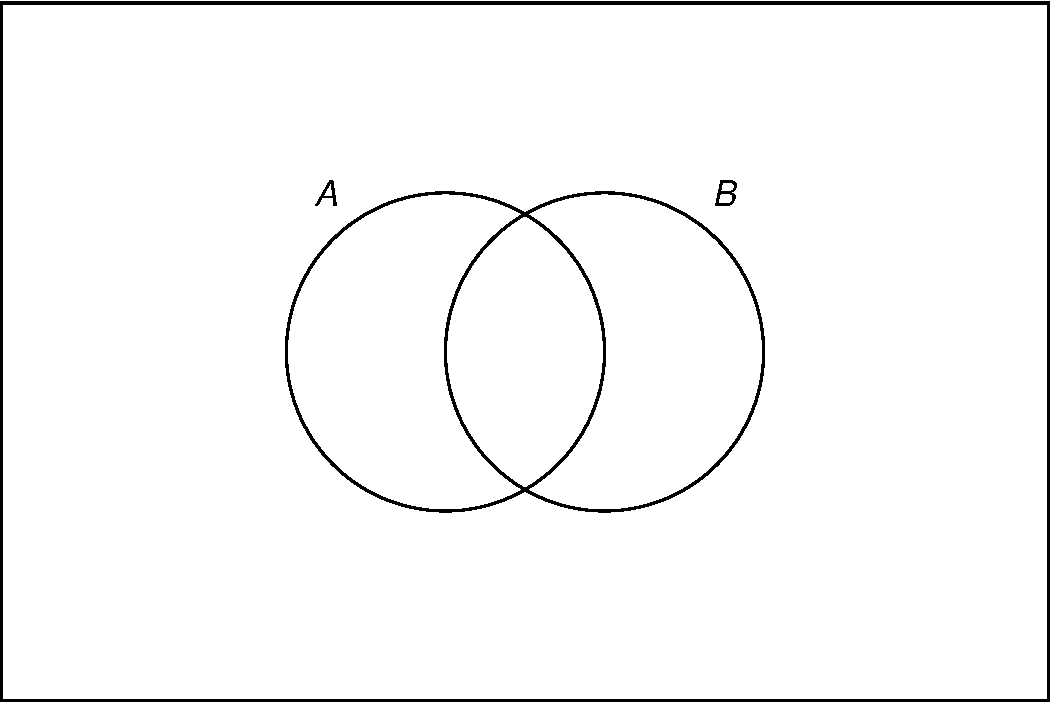
\includegraphics{_main_files/figure-latex/unnamed-chunk-55-1} \caption[The Tautology Rule]{The Tautology Rule. Every point falls in either the $A$ region or the $\neg A$ region, so $\p(A \vee \neg A) = 1$.}\label{fig:unnamed-chunk-55}
\end{marginfigure}

\newthought{A} tautology is a proposition that must be true, so its
probability is always 1.

\begin{description}
\item[The Tautology Rule]
\(\p(T) = 1\) for every tautology \(T\).
\end{description}

For example, \(A \vee \neg A\) is a tautology, so
\(\p(A \vee \neg A) = 1\). In terms of an Euler diagram, the \(A\) and
\(\neg A\) regions together take up the whole diagram. To put it a bit
colourfully,
\(\p(A \vee \neg A) = \color{bookred}{\blacksquare}\color{black}{} + \color{bookblue}{\blacksquare}\color{black}{} = 1\).

\newthought{The} flipside of a tautology is a contradiction, a
proposition that can't possibly be true. So it has probability 0.

\begin{description}
\item[The Contradiction Rule]
\(\p(C) = 0\) for every contradiction \(C\).
\end{description}

For example, \(A \wedge \neg A\) is a contradiction, so
\(\p(A \wedge \neg A) = 0\). In terms of our Euler diagram, there is no
region where \(A\) and \(\neg A\) overlap. So the portion the diagram
devoted to \(A \wedge \neg A\) is nil, zero.

\newthought{Equivalent} propositions are true under exactly the same
circumstances (and false under exactly the same circumstances). So they
have the same chance of being true (ditto false).

\begin{marginfigure}
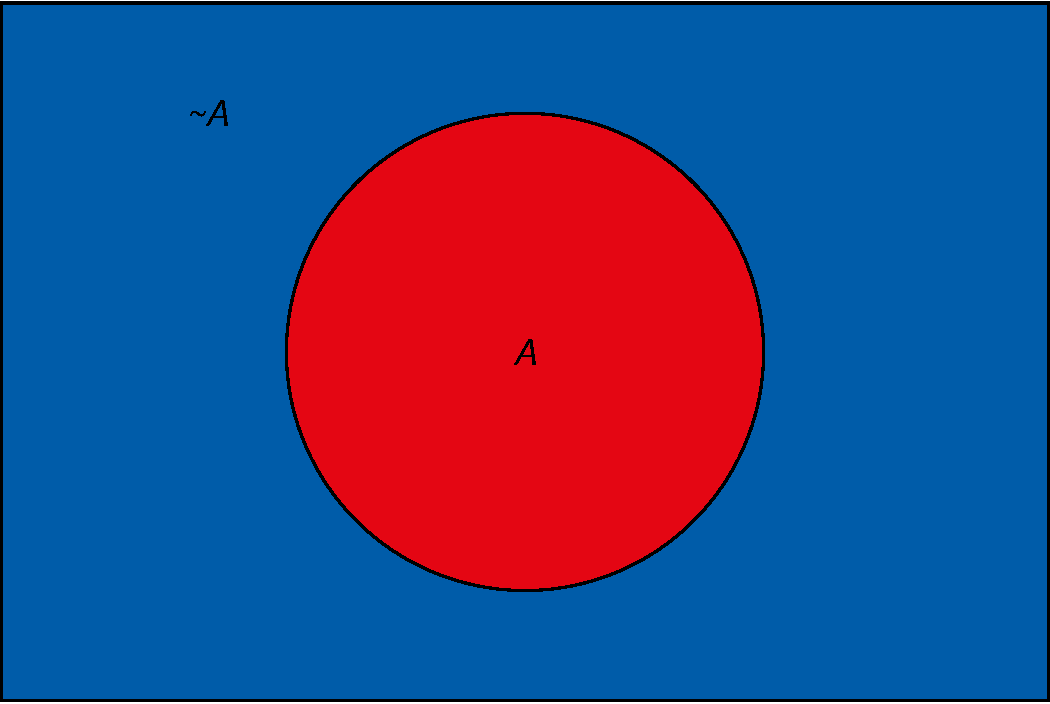
\includegraphics{_main_files/figure-latex/unnamed-chunk-56-1} \caption[The Equivalence Rule]{The Equivalence Rule. The $A \vee B$ region is identical to the $B \vee A$ region, so they have the same probability.}\label{fig:unnamed-chunk-56}
\end{marginfigure}

\begin{description}
\item[The Equivalence Rule]
\(\p(A) = \p(B)\) if \(A\) and \(B\) are logically equivalent.
\end{description}

For example, \(A \vee B\) is logically equivalent to \(B \vee A\), so
\(\p(A \vee B) = \p(B \vee A)\).

In terms of an Euler diagram, the \(A \vee B\) region is exactly the
same as the \(B \vee A\) region: the red region. So both propositions
take up the same amount of space in the diagram.

\hypertarget{the-language-of-events}{%
\section{The Language of Events}\label{the-language-of-events}}

\newthought{In} math and statistics books you'll often see a lot of the
same concepts from this chapter introduced in different language.
Instead of propositions, they'll discuss \emph{events}, which are sets
of possible outcomes.

For example, the roll of a six-sided die has six possible outcomes:
\(1, 2, 3, 4, 5, 6\). And the event of the die landing on an even number
is the set \(\{2, 4, 6\}\).

In this way of doing things, rather than consider the probability that a
proposition \(A\) is true, we consider the probability that event \(E\)
occurs. Instead of considering a conjunction of propositions like
\(A \,\&\, B\), we consider the \emph{intersection} of two events,
\(E \cap F\). And so on.

If you're used to seeing probability presented this way, there's an easy
way to translate into logic-ese. For any event \(E\), there's the
corresponding proposition that event \(E\) occurs. And you can translate
the usual set operations into logic as follows:

\begin{longtable}[]{@{}cc@{}}
\caption{\label{tab:unnamed-chunk-57}Translating between events and
propositions}\tabularnewline
\toprule
Events & Propositions\tabularnewline
\midrule
\endfirsthead
\toprule
Events & Propositions\tabularnewline
\midrule
\endhead
\(E^c\) & \(\sim\! A\)\tabularnewline
\(E \cap F\) & \(A \,\&\, B\)\tabularnewline
\(E \cup F\) & \(A \vee B\)\tabularnewline
\bottomrule
\end{longtable}

We won't use the language of events in this book. I'm just mentioning it
in case you've come across it before and you're wondering how it
connects. If you've never seen it before, you can safely ignore this
section.

\hypertarget{summary-1}{%
\section{Summary}\label{summary-1}}

\newthought{In} this chapter we learned how to represent probabilities
of propositions using the \(Pr(\ldots)\) operator. We also learned some
fundamental rules of probability.

There were three rules corresponding to the concepts of tautology,
contradiction, and equivalence.

\begin{itemize}
\tightlist
\item
  \(\p(T) = 1\) for every tautology \(T\).
\item
  \(\p(C) = 0\) for every contradiction \(C\).
\item
  \(\p(A) = \p(B)\) if \(A\) and \(B\) are logically equivalent.
\end{itemize}

And there were two rules corresponding to the connectives \(\wedge\) and
\(\vee\).

\begin{itemize}
\tightlist
\item
  \(Pr(A \vee B) = Pr(A) + Pr(B)\), if \(A\) and \(B\) are mutually
  exclusive.
\item
  \(Pr(A \wedge B) = Pr(A) \times Pr(B)\), if \(A\) and \(B\) are
  independent.
\end{itemize}

The restrictions on these two rules are essential. If you ignore them,
you will get wrong answers.

\hypertarget{exercises-4}{%
\section*{Exercises}\label{exercises-4}}
\addcontentsline{toc}{section}{Exercises}

\begin{enumerate}
\item
  What is the probability of each of the following propositions?

  \begin{enumerate}
  \def\labelenumii{\alph{enumii}.}
  \tightlist
  \item
    \(A \wedge (B \wedge \neg A)\)
  \item
    \(\neg (A \wedge \neg A)\)
  \end{enumerate}
\item
  Give an example of each of the following:

  \begin{enumerate}
  \def\labelenumii{\alph{enumii}.}
  \tightlist
  \item
    Two statements that are mutually exclusive.
  \item
    Two statements that are independent.
  \end{enumerate}
\item
  For each of the following, say whether it is true or false.

  \begin{enumerate}
  \def\labelenumii{\alph{enumii}.}
  \tightlist
  \item
    If propositions are independent, then they must be mutually
    exclusive.
  \item
    Independent propositions usually aren't mutually exclusive.
  \item
    If propositions are mutually exclusive, then they must be
    independent.
  \item
    Mutually exclusive propositions usually aren't independent.
  \end{enumerate}
\item
  Assume \(Pr(A \wedge B)=1/3\) and \(Pr(A \wedge \neg B)=1/5\). Answer
  each of the following:

  \begin{enumerate}
  \def\labelenumii{\alph{enumii}.}
  \tightlist
  \item
    What is \(Pr((A \wedge B) \vee (A \wedge \neg B))\)?
  \item
    What is \(Pr(A)\)?
  \item
    Are \((A \wedge B)\) and \((A \wedge \neg B)\) independent?
  \end{enumerate}
\item
  Suppose \(A\) and \(B\) are independent, and \(A\) and \(C\) are
  mutually exclusive. Assume \(\p(A) = 1/3, \p(B) = 1/6, \p(C) = 1/9\),
  and answer each of the following:

  \begin{enumerate}
  \def\labelenumii{\alph{enumii}.}
  \tightlist
  \item
    What is \(\p(A \wedge C)\)?
  \item
    What is \(\p((A \wedge B) \vee C)\)?
  \item
    Must \(\p(A \wedge B) = 0\)?
  \end{enumerate}
\item
  Consider the following argument:

  \begin{argument}
   If a coin is fair, then the probability of getting at least one heads in
   a sequence of four tosses is quite high: above 90\%.

   \begin{center}\rule{0.5\linewidth}{\linethickness}\end{center}

   Therefore, if a fair coin has landed tails three times in a row, the
   next toss will probably land heads.
   \end{argument}

  Answer each of the following questions.

  \begin{enumerate}
  \def\labelenumii{\alph{enumii}.}
  \tightlist
  \item
    Is the premise of this argument true?
  \item
    Is the argument valid?
  \item
    Is the argument sound?
  \end{enumerate}
\item
  The Addition Rule can be extended to three propositions. If \(A\),
  \(B\), and \(C\) are all mutually exclusive with one another, then

  \[ \p(A \vee B \vee C) = \p(A) + \p(B) + \p(C).\]

  Explain why this rule is correct. Would the same idea extend to four
  mutually exclusive propositions? To five?

  (Hint: there's more than one way to do this. You can use an Euler
  diagram. Or you can derive the new rule from the original one, by
  thinking of \(A \vee B \vee C\) as a disjunction of \(A \vee B\) and
  \(C\).)
\item
  You have a biased coin, where each toss has a \(3/5\) chance of
  landing heads. But each toss is independent of the others. Suppose
  you're going to flip the coin \(1,000\) times. The first 998 tosses
  all land tails. What is the probability at least one of the last two
  flips will be tails?
\end{enumerate}

\hypertarget{conditional-probability}{%
\chapter{Conditional Probability}\label{conditional-probability}}

\newthought{The} chances of crashing your car are pretty low, but
they're considerably higher if you're drunk. Probabilities change
depending on the conditions.

We symbolize this idea by writing \(\p(A \given B)\), the probability
that \(A\) is true \emph{given} that \(B\) is true. And we call this
kind of probability \textbf{\emph{conditional probability}}.

\begin{marginfigure}
To say \(B\) increases the chance of \(A\) we write
\(\p(A \given B) \gt \p(A)\). And to say \(B\) doubles the chance of
\(A\) write \(\p(A \given B) = 2 \times \p(A)\).
\end{marginfigure}

For example, to say the probability of \(A\) given \(B\) is 30\%, we
write: \[ \p(A \given B) = .3. \] But how do we calculate conditional
probabilities?

\hypertarget{calculating-conditional-probability}{%
\section{Calculating Conditional
Probability}\label{calculating-conditional-probability}}

\begin{marginfigure}
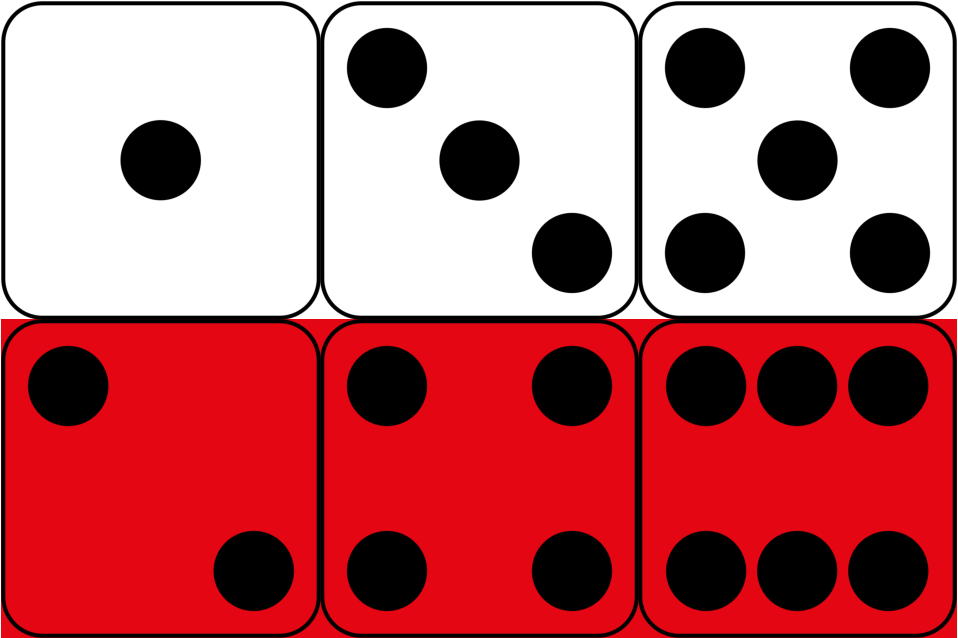
\includegraphics{_main_files/figure-latex/unnamed-chunk-60-1} 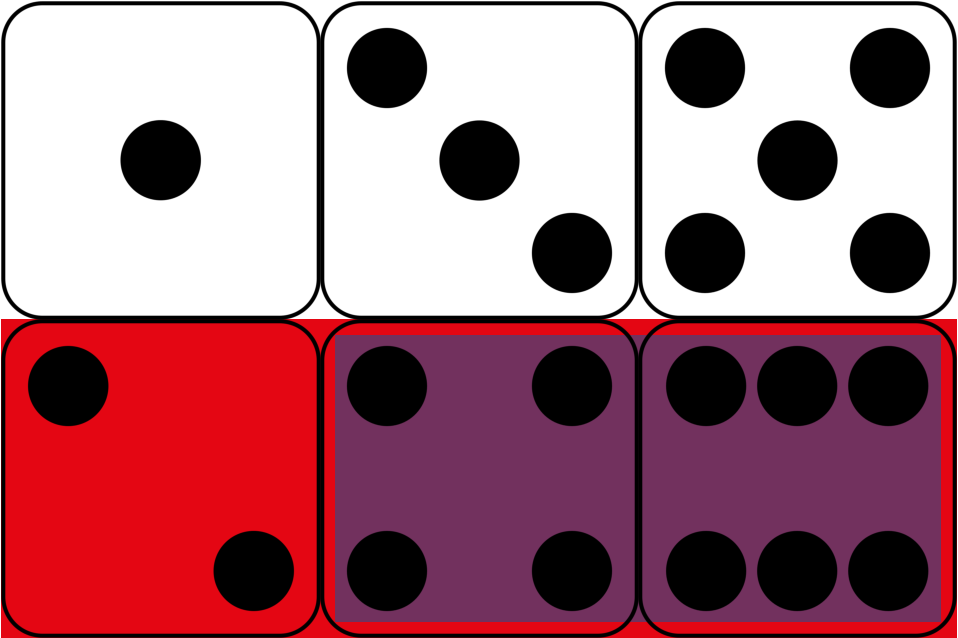
\includegraphics{_main_files/figure-latex/unnamed-chunk-60-2} \caption[Conditional probability in a fair die roll]{Conditional probability in a fair die roll}\label{fig:unnamed-chunk-60}
\end{marginfigure}

Suppose I roll a fair, six-sided die behind a screen. You can't see the
result, but I tell you it's an even number. What's the probability it's
also a ``high'' number: either a \(4\), \(5\), or \(6\)?

Maybe you figured the correct answer: \(2/3\). But why is that correct?
Because, out of the three even numbers (\(2\), \(4\), and \(6\)), two of
them are high (\(4\) and \(6\)). And since the die is fair, we expect it
to land on a high number \(2/3\) of the times it lands on an even
number.

This hints at a formula for \(\p(A \given B)\).

\begin{description}
\item[Conditional Probability]
\[ \p(A \given B) = \frac{\p(A \wedge B)}{\p(B)}. \]
\end{description}

In the die-roll example, we considered how many of the \(B\)
possibilities were also \(A\) possibilities. Which means we divided
\(\p(A \wedge B)\) by \(\p(B)\).

In fact, this formula is our official definition for the concept of
conditional probability. When we write the sequence of symbols
\(\p(A \given B)\), it's really just shorthand for the fraction
\(\p(A \wedge B) / \p(B)\).

\begin{marginfigure}
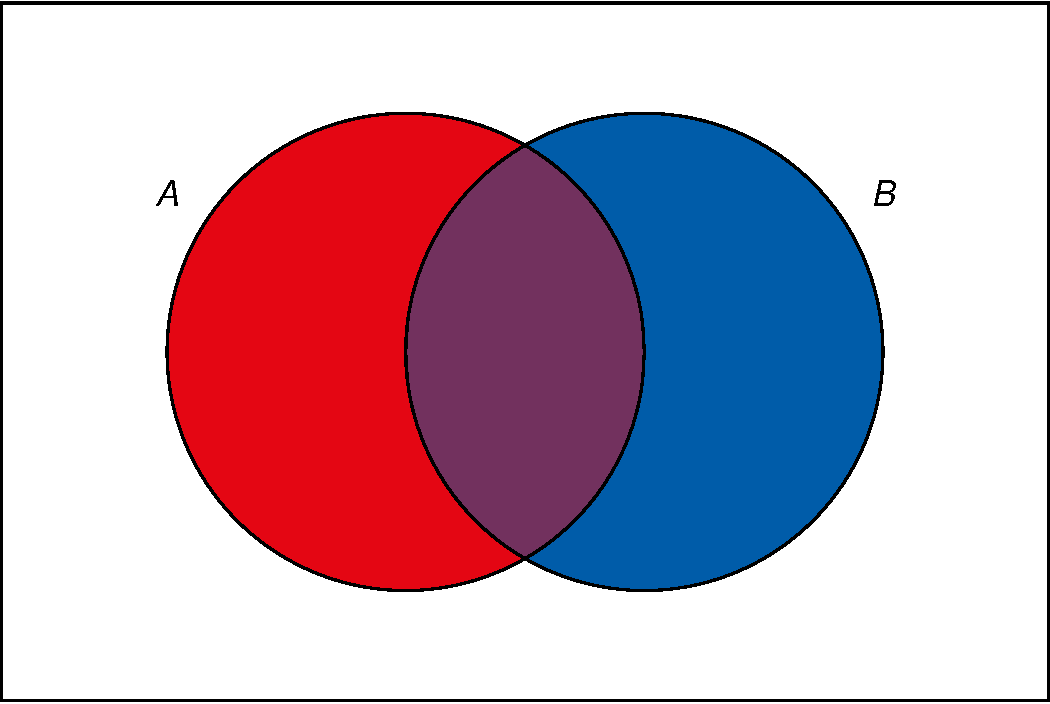
\includegraphics{_main_files/figure-latex/condprob-1} \caption[Conditional probability is the size of the $A \wedge B$ region compared to the entire $B$ region]{Conditional probability is the size of the $A \wedge B$ region compared to the entire $B$ region.}\label{fig:condprob}
\end{marginfigure}

In terms of an Euler diagram (Figure \ref{fig:condprob}), the definition
of conditional probability compares the size of the purple
\(A \wedge B\) region to the size of the whole \(B\) region, purple and
blue together. If you don't mind getting a little colourful with your
algebra: \[
  \p(A \given B) = \frac{\color{bookpurple}{\blacksquare}}{\color{bookpurple}{\blacksquare} + \color{bookblue}{\blacksquare}}.
\] So the definition works because, informally speaking,
\(\p(A \wedge B)/\p(B)\) is the proportion of the \(B\) outcomes that
are also \(A\) outcomes.\footnote{The comedian Steven Wright once
  quipped that ``black holes are where God divided by zero.''}

\newthought{Dividing} by zero is a common pitfall with conditional
probability. Notice how the definition of \(\p(A \given B)\) depends on
\(\p(B)\) being larger than zero. If \(\p(B) = 0\), then the formula
\[ \p(A \given B) = \frac{\p(A \wedge B)}{\p(B)} \] doesn't even make
any sense. There is no number that results from the division on the
right hand side.\footnote{There are alternative mathematical systems of
  probability, where conditional probability is defined differently to
  avoid this problem. But in this book we'll stick to the standard
  system. Where there's just no such thing as ``the probability of \(A\)
  given \(B\)'' when \(B\) has zero probability.}

In such cases we say that \(\p(A \given B)\) is \emph{undefined}. It's
not zero, or some special number. It just isn't a number.

\hypertarget{conditional-probability-trees}{%
\section{Conditional Probability \&
Trees}\label{conditional-probability-trees}}

\newthought{We} already encountered conditional probabilities
informally, when we used a tree diagram to solve
\protect\hyperlink{the-monty-hall-problem}{the Monty Hall problem}.

In a tree diagram, each branch represents a possible outcome. The number
placed on that branch represents the chance of that outcome occurring.
But that number is based on the assumption that all branches leading up
to it occur. So the probability on that branch is conditional on all
previous branches.

For example, suppose there are two urns of coloured marbles:

\begin{itemize}
\tightlist
\item
  Urn X contains 3 black marbles, 1 white.
\item
  Urn Y contains 1 black marble, 3 white.
\end{itemize}

I flip a fair coin to decide which urn to draw from, heads for Urn B and
tails for Urn W. Then I draw one marble at random.

\begin{figure}
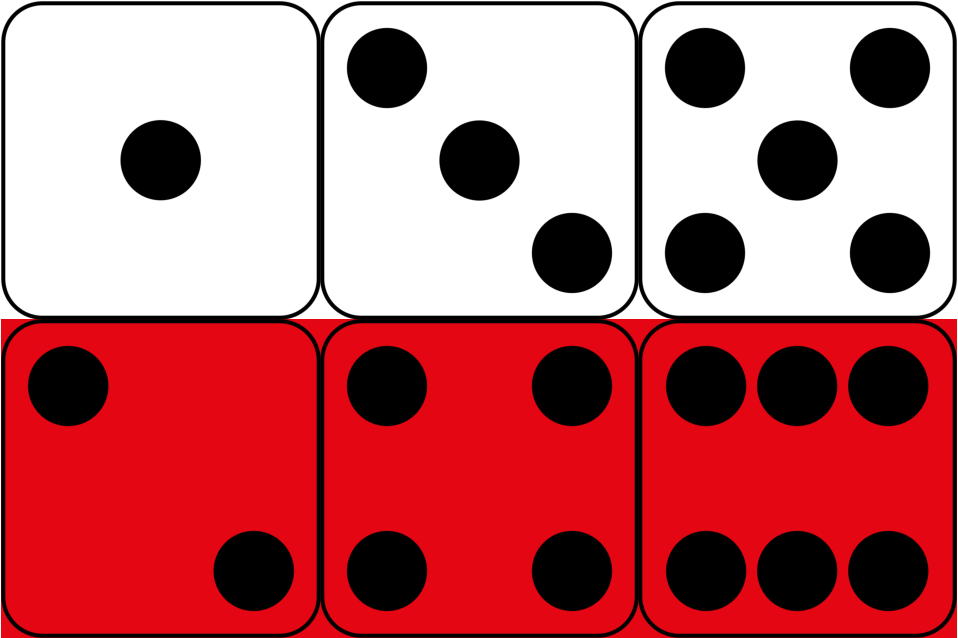
\includegraphics{_main_files/figure-latex/unnamed-chunk-61-1} \caption[Tree diagram for an urn problem]{Tree diagram for an urn problem}\label{fig:unnamed-chunk-61}
\end{figure}

The probability of drawing a black marble on the top path is \(3/4\)
because we are assuming the coin landed heads, and thus I'm drawing from
Urn X. If the coin lands tails instead, and I draw from Urn Y, then the
chance of a black marble is instead \(1/4\). So these quantities are
conditional probabilities: \[
  \begin{aligned}
    \p(B \given H) &= 3/4,\\
    \p(B \given T) &= 1/4.
  \end{aligned}
\]

Notice, though, the first branch in a tree diagram is different. In the
\(H\)-vs.-\(T\) branch, the probabilities are \emph{un}conditional,
since there are no previous branches for them to be conditional on.

\hypertarget{more-examples}{%
\section{More Examples}\label{more-examples}}

\newthought{Imagine} an urn contains marbles of three different colours:
20 are red, 30 are blue, and 40 are green. I draw a marble at random.
What is \(\p(R \given \neg B)\), the probability it's red given that
it's not blue? \[
  \begin{aligned}
    \p(R \given \neg B) &= \frac{\p(R \wedge \neg B)}{\p(\neg B)}\\
                        &= \frac{\p(R)}{\p(\neg B)}\\
                        &= \frac{20/90}{60/90}\\
                        &= 1/3.
  \end{aligned}
\] This calculation relies on the fact that \(R \wedge \neg B\) is
logically equivalent to \(R\). A red marble is automatically not blue,
so \(R\) is true under exactly the same circumstances as
\(R \wedge \neg B\). The
\protect\hyperlink{tautologies-contradictions-and-equivalent-propositions}{Equivalence
Rule} thus tells us \(\p(R \wedge \neg B) = \p(R)\).

\newthought{Suppose} a university has 10,000 students, and each student
is studying under one of four broad headings: Humanities, Social
Sciences, STEM, or Professional. Within each of these categories, the
number of students with an average grade of A, B, C, or D is as follows:

\begin{longtable}[]{@{}lcccc@{}}
\toprule
& Humanities & Social Sciences & STEM & Professional\tabularnewline
\midrule
\endhead
A & 200 & 600 & 400 & 900\tabularnewline
B & 500 & 800 & 1600 & 900\tabularnewline
C & 250 & 400 & 1500 & 750\tabularnewline
D & 50 & 200 & 500 & 450\tabularnewline
\bottomrule
\end{longtable}

What is the probability a randomly selected student will have an A
average, given that they are studying either Humanities or Social
Sciences? \[
  \begin{aligned}
    \p(A \given H \vee S) &= \frac{\p(A \wedge (H \vee S))}{\p(H \vee S)}\\
                           &= \frac{800/10,000}{3,000/10,000}\\
                           &= 4/15.
  \end{aligned}
\]

What about the reverse probability, that a student is studying either
Humanities or Social Sciences given that they have an A average? \[
  \begin{aligned}
    \p(H \vee S \given A) &= \frac{\p((H \vee S) \wedge A)}{\p(A)}\\
                           &= \frac{800/10,000}{2,100/10,000}\\
                           &= 8/21.
  \end{aligned}
\] Notice how we get a different number now.

\hypertarget{order-matters}{%
\section{Order Matters}\label{order-matters}}

\newthought{In} general, the probability of \(A\) given \(B\) will be
different from the probability of \(B\) given \(A\). These are different
concepts.

For example, university students are usually young, but young people
aren't usually university students. Most aren't even old enough to be in
university. So the probability someone is young given they are in
university is high. But the probability someone is in university given
that they are young is low. So \(\p(Y \given U) \neq \p(U \given Y)\).

Once in a while we do find cases where
\(\p(A \given B) = \p(B \given A)\). For example, suppose we throw a
dart at random at a circular board, divided into four quadrants. The
chance the dart will land on the left half given that it lands on the
top half is the same as the chance it lands on the top half given it
lands on the left. Both probabilities are \(1/2\).

But this kind of thing is the exception rather than the rule. Usually,
\(\p(A \given B)\) will be a different number from \(\p(B \given A)\).
So it's important to remember how order matters.

\begin{warning}
When we write \(\p(A \given B)\), we are discussing the probability of
\(A\). But we are discussing it under the assumption that \(B\) is true.
\end{warning}

\hypertarget{declaring-independence}{%
\section{Declaring Independence}\label{declaring-independence}}

\newthought{We} explained independence informally back in
\protect\hyperlink{independence-1}{Chapter 4}: \(A\) and \(B\) are
independent if the truth of one doesn't change the probability of the
other. Now that we've formally defined conditional probability, we can
formally define independence too.

\begin{description}
\item[Independence]
\(A\) is independent of \(B\) if \(\p(A \given B) = \p(A)\) and
\(\p(A) > 0\).
\end{description}

In other words, they're independent if \(A\)'s probability is the same
after \(B\) is given as it was before (and not just for the silly reason
that there was no chance of \(A\) being true to begin with).

Now we can establish three useful facts about independence.

\newthought{The} first is summed up in the mantra ``independence means
multiply''. This actually has two parts.

We already learned the first part with the Multiplication Rule: if \(A\)
is independent of \(B\), then \(\p(A \wedge B) = \p(A)\p(B)\). Except
now we can see why this rule holds, using the definition of conditional
probability and some algebra: \[
  \begin{aligned}
    \p(A \given B)      &= \frac{\p(A \wedge B)}{\p(B)} & \mbox{by definition}\\
    \p(A \given B)\p(B) &= \p(A \wedge B)               & \mbox{by algebra}\\
    \p(A)\p(B)          &= \p(A \wedge B)               & \mbox{by independence}.
  \end{aligned}
\]

The second part of the ``independence means multiply'' mantra is new
though. It basically says that the reverse also holds. As long as
\(\p(A) > 0\) and \(\p(B) > 0\), if \(\p(A \wedge B) = \p(A)\p(B)\),
then \(A\) is independent of \(B\).

Bottom line: as long as there are no zeros to worry about, independence
is the same thing as \(\p(A \wedge B) = \p(A)\p(B)\).

\newthought{Second,} independence is symmetric. If \(A\) is independent
of \(B\) then \(B\) is independent of \(A\). Informally speaking, if
\(B\) makes no difference to \(A\)'s probability, then \(A\) makes no
difference to \(B\)'s probability.

This is why we often say ``\(A\) and \(B\) are independent'', without
specifying which is independent of which. Since independence goes both
ways, they're automatically independent of each other.

\newthought{Third,} independence extends to negations. If \(A\) is
independent of \(B\), then it's also independent of \(\neg B\) (as long
as \(\p(\neg B) > 0\), so that \(\p(A \given \neg B)\) is well-defined).

Notice, this also means that if \(A\) is independent of \(B\), then
\(\neg A\) is independent of \(\neg B\) (as long as \(\p(\neg A) > 0\)).

\newthought{So} far our definition of independence only applies to two
propositions. We can extend it to three as follows:

\begin{description}
\item[Three-way Independence]
\(A\), \(B\), and \(C\) are independent if

\begin{enumerate}
\def\labelenumi{\roman{enumi}.}
\tightlist
\item
  \(A\) is independent of \(B\), \(A\) is independent of \(C\), and
  \(B\) is independent of \(C\), and
\item
  \(\p(A \wedge B \wedge C) = \p(A)\p(B)\p(C)\).
\end{enumerate}
\end{description}

In other words, a trio of propositions is independent if each pair of
them is independent, and the multiplication rule applies to their
conjunction. The same idea can be extended to define independence for
four propositions, five, etc.

\hypertarget{ch6ex}{%
\section*{Exercises}\label{ch6ex}}
\addcontentsline{toc}{section}{Exercises}

\begin{enumerate}
\item
  Answer each of the following:

  \begin{enumerate}
  \def\labelenumii{\alph{enumii}.}
  \tightlist
  \item
    On a fair die with six sides, what is the probability of rolling a
    low number (1, 2, or 3) given that you roll an even number.
  \item
    On a fair die with eight sides, what is the probability of rolling
    an even number given that you roll a high number (5, 6, 7, or 8)?
  \end{enumerate}
\item
  Suppose \(\p(B) = 4/10\), \(\p(A) = 7/10\), and
  \(\p(B \wedge A) = 2/10\). What are each of the following
  probabilities?

  \begin{enumerate}
  \def\labelenumii{\alph{enumii}.}
  \tightlist
  \item
    \(\p(A \given B)\)
  \item
    \(\p(B \given A)\)
  \end{enumerate}
\item
  Five percent of tablets made by the company Ixian have factory
  defects. Ten percent of the tablets made by their competitor company
  Guild do. A computer store buys \(40\%\) of its tablets from Ixian,
  and \(60\%\) from Guild.

  \begin{marginfigure}
   This exercise and the next one are based on very similar exercises from
   Ian Hacking's wonderful book, \emph{An Introduction to Probability and
   Inductive Logic}.
   \end{marginfigure}

  Draw a probability tree to answer the following questions.

  \begin{enumerate}
  \def\labelenumii{\alph{enumii}.}
  \tightlist
  \item
    What is the probability a randomly selected tablet in the store is
    made by Ixian and has a factory defect?
  \item
    What is the probability a randomly selected tablet in the store has
    a factory defect?
  \item
    What is the probability a tablet from this store is made by Ixian,
    given that it has a factory defect?
  \end{enumerate}
\item
  In the city of Elizabeth, the neighbourhood of Southside has lots of
  chemical plants. \(2\%\) of Elizabeth's children live in Southside,
  and \(14\%\) of those children have been exposed to toxic levels of
  lead. Elsewhere in the city, only \(1\%\) of the children have toxic
  levels of exposure.

  Draw a probability tree to answer the following questions.

  \begin{enumerate}
  \def\labelenumii{\alph{enumii}.}
  \tightlist
  \item
    What is the probability that a randomly chosen child from Elizabeth
    lives in Southside and has toxic levels of lead exposure?
  \item
    What is the probability that a randomly chosen child from Elizabeth
    has toxic levels of lead exposure?
  \item
    What is the probability that a randomly chosen child from Elizabeth
    who has toxic levels of lead exposure lives in Southside?
  \end{enumerate}
\item
  Imagine 100 prisoners are sentenced to death. 70 of them are housed in
  cell block A, the other 30 are in cell block B. Of the prisoners in
  cell block A, 9 are innocent. Only 1 prisoner in cell block B is
  innocent.

  The law requires that one prisoner be pardoned. The lucky prisoner
  will be selected by flipping a fair coin to choose either cell block A
  or B. Then a fair lottery will be used to select a random prisoner
  from the chosen cell block.

  What is the probability the pardoned prisoner comes from cell block A
  if she is innocent? Answer each of the following to find out.

  \(I\) = The pardoned prisoner is innocent.\\
  \(A\) = The pardoned prisoner comes from cell block A.

  \begin{enumerate}
  \def\labelenumii{\alph{enumii}.}
  \tightlist
  \item
    What is \(Pr(I \given A)\)?
  \item
    What is \(Pr(A \wedge I)\)?
  \item
    What is \(Pr(I \given B)\)?
  \item
    What is \(Pr(B \wedge I)\)?
  \item
    What is \(Pr(I)\)?
  \item
    What is \(Pr(A \given I)\)?
  \item
    Draw a probability tree to visualize and verify your calculations.
  \end{enumerate}
\item
  Suppose \(A\), \(B\), and \(C\) are independent, and they each have
  the same probability: \(1/3\). What is \(\p(A \wedge B \given C)\)?
\item
  If \(A\) and \(B\) are mutually exclusive, what is \(\p(A \given B)\)?
  Justify your answer using the definition of conditional probability.
\item
  Which of the following situations is impossible? Justify your answer.

  \begin{enumerate}
  \def\labelenumii{\alph{enumii}.}
  \tightlist
  \item
    \(\p(A) = 1/2, \p(A \given B) = 1/2, \p(B \given A) = 1/2\).
  \item
    \(\p(A) = 1/2, \p(A \given B) = 1, \p(A \given \neg B) = 1\).
  \end{enumerate}
\item
  Is the following statement true or false: if \(A\) and \(B\) are
  mutually exclusive, then
  \(Pr(A \vee B \given C) = Pr(A \given C) + Pr(B \given C)\). Justify
  your answer.
\item
  Justify the second part of the ``independence means multiply'' mantra:
  if \(\p(A) > 0\), \(\p(B) > 0\), and \(\p(A \wedge B) = \p(A) \p(B)\),
  then \(A\) is independent of \(B\).

  Hint: start by supposing \(\p(A) > 0\), \(\p(B) > 0\), and
  \(\p(A \wedge B) = \p(A)\p(B)\). Then apply some algebra and the
  definition of conditional probability.
\item
  Justify the claim that independence is symmetric: if \(A\) is
  independent of \(B\), then \(B\) is independent of \(A\).

  Hint: start by supposing that \(A\) is independent of \(B\). Then
  write out \(\p(A \given B)\) and apply the definition of conditional
  probability.
\end{enumerate}

\hypertarget{calculating-probabilities-part-ii}{%
\chapter{Calculating Probabilities, Part
II}\label{calculating-probabilities-part-ii}}

\newthought{We} learned rules for \(\vee\) and for \(\wedge\) back in
\protect\hyperlink{calculating-probabilities}{Chapter 5}:

\begin{description}
\item[The Addition Rule]
\(\p(A \vee B) = \p(A) + \p(B)\) if \(A\) and \(B\) are mutually
exclusive.
\item[The Multiplication Rule]
\(\p(A \& B) = \p(A) \times \p(B)\) if \(A\) and \(B\) are independent.
\end{description}

In this chapter we'll learn new, more powerful rules for \(\vee\) and
\(\wedge\). But we'll start with negation, a rule for calculating
\(\p(\neg A)\).

\hypertarget{the-negation-rule}{%
\section{The Negation Rule}\label{the-negation-rule}}

\begin{marginfigure}
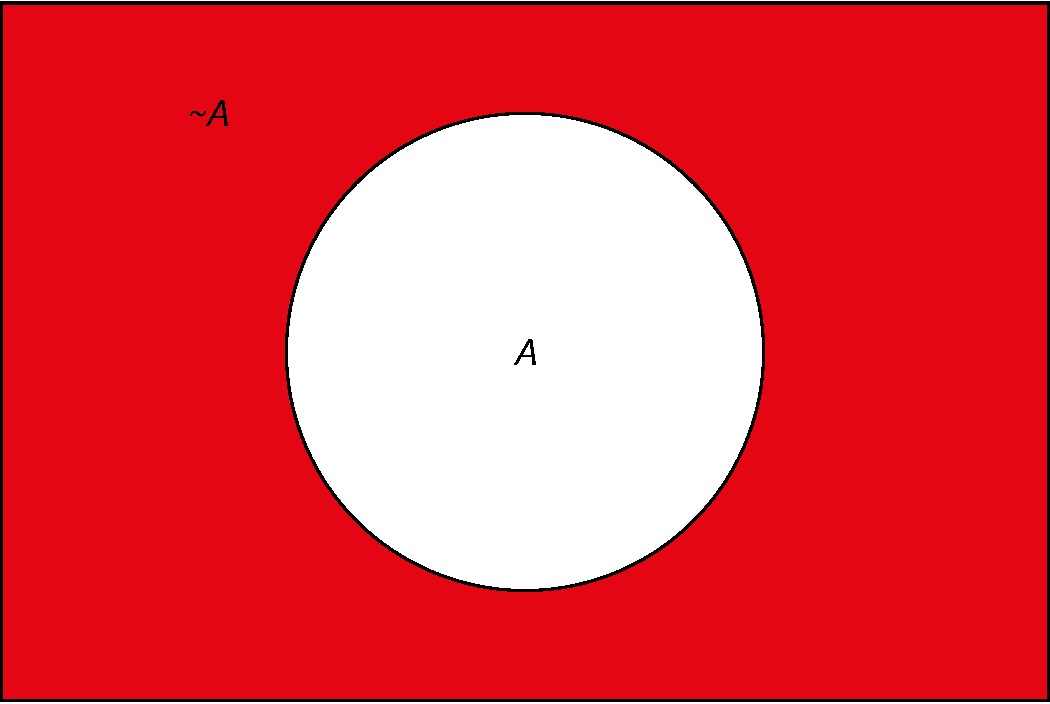
\includegraphics{_main_files/figure-latex/unnamed-chunk-65-1} \caption[The Negation Rule]{The Negation Rule. $\p(\neg A) = 1 - \p(A)$.}\label{fig:unnamed-chunk-65}
\end{marginfigure}

If there's a 70\% chance of rain, then there's a 30\% chance it won't
rain. In symbols, if \(\p(R) = .7\) then \(\p(\neg R) = .3\). So the
rule for \(\p(\neg A)\) is:

\begin{description}
\item[The Negation Rule]
\(\p(\neg A) = 1 - \p(A)\).
\end{description}

In terms of an Euler diagram, the probability of \(\neg A\) is the size
of the red region. So \(\p(\neg A)\) is \(1 - \p(A)\).

\newthought{It's important} to notice that this rule can be flipped
around, to calculate the probability of a positive statement: \[ 
  \p(A) = 1 - \p(\neg A).
\] Sometimes we really want to know the probability of \(A\), \(\p(A)\),
but it turns out to be much easier to calculate \(\p(\neg A)\) first.
Then we use this flipped version of the negation rule to get what we're
after.

\hypertarget{the-general-addition-rule}{%
\section{The General Addition Rule}\label{the-general-addition-rule}}

\newthought{The} Addition Rule for calculating \(\p(A \vee B)\) depends
on \(A\) and \(B\) being mutually exclusive. What if they're not? Then
we can use:

\begin{description}
\item[The General Addition Rule]
\(\p(A \vee B) = \p(A) + \p(B) - \p(A \wedge B)\).
\end{description}

This rule always applies, whether \(A\) and \(B\) are mutually exclusive
or not.

\begin{marginfigure}
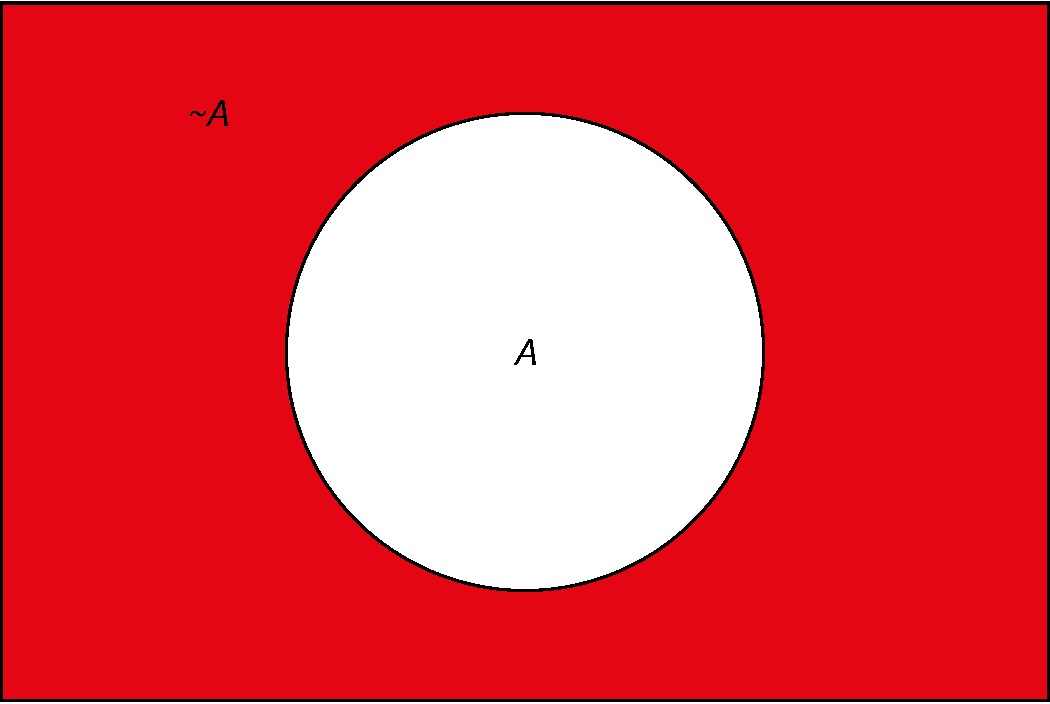
\includegraphics{_main_files/figure-latex/unnamed-chunk-66-1} \caption[The General Addition Rule in an Euler diagram]{The General Addition Rule in an Euler diagram.}\label{fig:unnamed-chunk-66}
\end{marginfigure}

To understand the rule, consider an Euler diagram where \(A\) and \(B\)
are not mutually exclusive. In terms of colour, the size of the
\(A \vee B\)-region is: \[ 
  \color{bookred}{\blacksquare}\color{black}{}
    \,+\,
  \color{bookpurple}{\blacksquare}\color{black}{}
    \,+\,
  \color{bookblue}{\blacksquare}\color{black}{}.
\] Which is the same as: \[
  (\color{bookred}{\blacksquare}\color{black}{}
    \,+\,
  \color{bookpurple}{\blacksquare}\color{black}{})
    \,+\, 
  (\color{bookblue}{\blacksquare}\color{black}{}
    \,+\,
  \color{bookpurple}{\blacksquare}\color{black}{}) 
    \,-\,
  \color{bookpurple}{\blacksquare}\color{black}{}.
\] In algebraic terms this is: \[ \p(A) + \p(B) - \p(A \wedge B).\]

To think of it another way, when we add \(\p(A) + \p(B)\) to get the
size of the \(A \vee B\) region, we double-count the \(A \wedge B\)
region. So we have to subtract out \(\p(A \wedge B)\) at the end.

\newthought{What} if there is no \(A \wedge B\) region? Then
\(\p(A \wedge B) = 0\), so subtracting it at the end has no effect. Then
we just have the old Addition Rule: \[
  \begin{aligned}
    \p(A \vee B) &= \p(A) + \p(B) - \p(A \wedge B)\\
                 &= \p(A) + \p(B) - 0\\
                 &= \p(A) + \p(B).\\
  \end{aligned}
\] And this makes sense. If there is no \(A \wedge B\) region, that
means \(A\) and \(B\) are mutually exclusive. So the old Addition Rule
applies.

That's why we call the new rule the \emph{General} Addition Rule. It
applies in general, even when \(A\) and \(B\) are not mutually
exclusive. And in the special case where they are mutually exclusive, it
gives the same result as the Addition Rule we already learned.

\newthought{A} tree diagram also works to explain the General Addition
Rule. Consider Figure \ref{fig:gatree}, where we start with branches for
\(A\) and \(\neg A\), then subdivide into branches for \(B\) and
\(\neg B\).

\begin{figure}
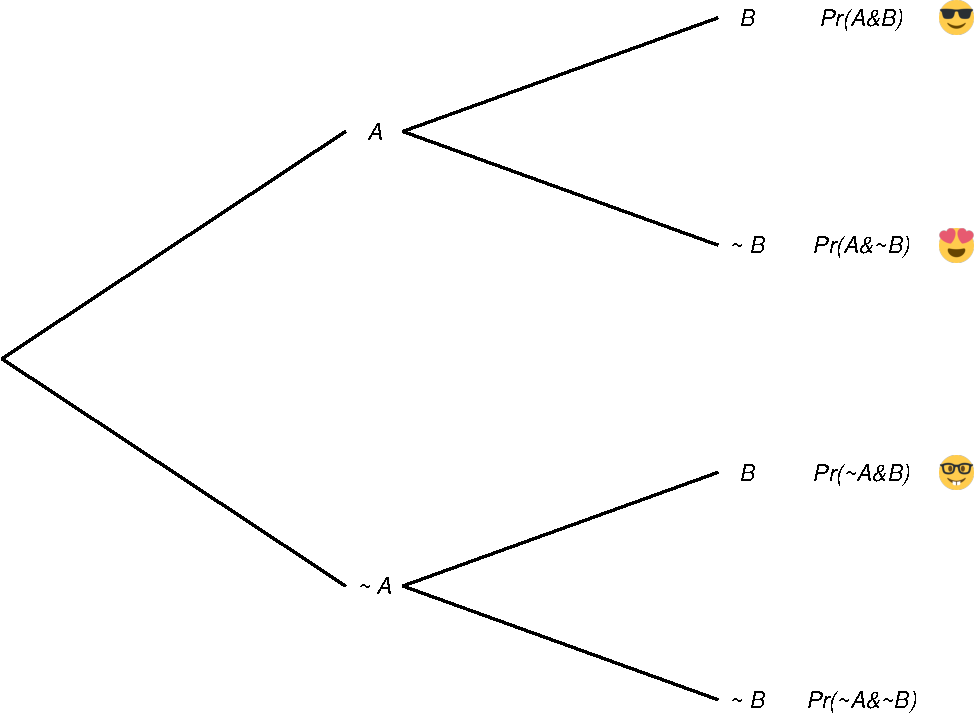
\includegraphics{_main_files/figure-latex/gatree-1} \caption[Tree diagram with the three $A \vee B$ leaves marked]{Tree diagram with the three $A \vee B$ leaves marked}\label{fig:gatree}
\end{figure}

There are three leaves where \(A \vee B\) is true, marked with emoji. If
we add \(\p(A) + \p(B)\), we're adding the two leaves where \(A\) is
true ( 
\includegraphics[width=0.18in]{img/emoji_shades_small} and

\includegraphics[width=0.18in]{img/emoji_hearts_small} ) to the two
leaves where \(B\) is true (

\includegraphics[width=0.18in]{img/emoji_shades_small} and

\includegraphics[width=0.18in]{img/emoji_nerd_small} ). So we've
double-counted the \(A \wedge B\) leaf (

\includegraphics[width=0.18in]{img/emoji_shades_small} ). To get
\(\p(A \vee B)\) then, we have to subtract one of those \(A \wedge B\)
leaves ( 
\includegraphics[width=0.18in]{img/emoji_shades_small} ).

\newthought{There} is a catch to the General Addition Rule. You need to
know \(\p(A \wedge B)\) in order to apply it. Sometimes that information
is given to us. But when it's not, we have to figure it out somehow. If
\(A\) and \(B\) are mutually exclusive, then it's easy:
\(\p(A \wedge B) = 0\). Or, if they're independent, then we can
calculate \(\p(A \wedge B) = \p(A) \times \p(B)\). But in other cases we
have to turn elsewhere.

\hypertarget{the-general-multiplication-rule}{%
\section{The General Multiplication
Rule}\label{the-general-multiplication-rule}}

\newthought{How} can we calculate \(\p(A \wedge B)\) in general?

\begin{description}
\item[The General Multiplication Rule]
\(\p(A \wedge B) = \p(A \given B) \p(B).\)
\end{description}

The intuitive idea is, if you want to know how likely it is \(A\) and
\(B\) will both turn out to be true, first ask yourself how likely \(A\)
is to be true \emph{if} \(B\) is true. Then weight the answer according
to \(B\)'s chances of being true.

Notice, if \(A\) and \(B\) are independent, then this rule just
collapses into the familiar Multiplication Rule we already learned. If
they're independent, then \(\p(A \given B) = \p(A)\) by definition. So
substituting into the General Multiplication Rule gives: \[
  \begin{aligned}
    \p(A \wedge B) &= \p(A \given B) \p(B)\\
                   &= \p(A) \p(B).
  \end{aligned}
\] Which is precisely the Multiplication Rule.

So we now have two rules for \(\wedge\). The first one only applies when
the two sides of the \(\wedge\) are independent. The second applies
whether they're independent or not. The second rule ends up being the
same as the first one when they are independent.

\newthought{A} tree diagram helps us understand this rule too. Recall
this problem from \protect\hyperlink{conditional-probability}{Chapter
6}, with two urns of coloured marbles:

\begin{itemize}
\tightlist
\item
  Urn X contains 3 black marbles, 1 white.
\item
  Urn Y contains 1 black marble, 3 white.
\end{itemize}

I flip a fair coin to decide which urn to draw from, heads for Urn X and
tails for Urn Y. Then I draw one marble at random.

\begin{figure}
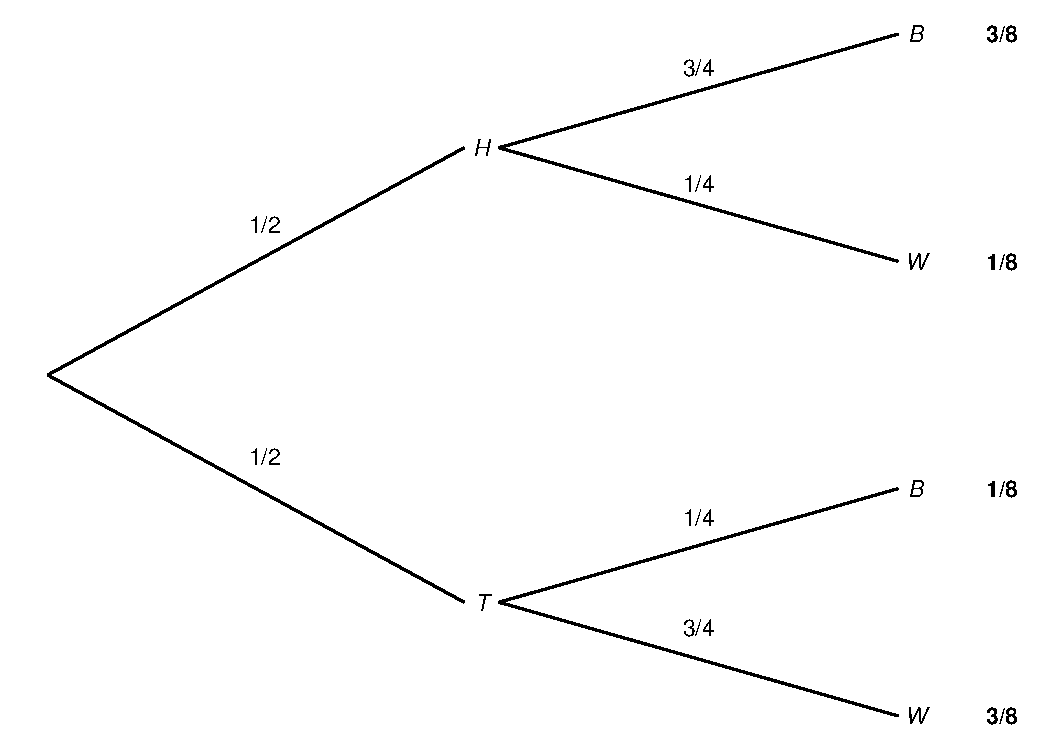
\includegraphics{_main_files/figure-latex/unnamed-chunk-68-7} \caption[Tree diagram for an urn problem]{Tree diagram for an urn problem}\label{fig:unnamed-chunk-68}
\end{figure}

Now suppose we want to know the probability the coin will land tails and
the marble drawn will be white, \(\p(T \wedge W)\). The General
Multiplication Rule tells us the answer is: \[
  \begin{aligned}
    \p(T \wedge W) &= \p(W \wedge T)\\
                   &= \p(W \given T) \p(T)\\
                   &= 3/4 \times 1/2\\
                   &= 3/8.
  \end{aligned}
\] In the tree diagram, this corresponds to following the bottom-most
path, multiplying the probabilities as we go. And this makes sense: half
the time the coin will land tails, and on \(3/4\) of those occasions the
marble drawn will be white. So, if we were to repeat the experiment
again and again, we would get tails followed by a white marble in \(3\)
out of every \(8\) trials.

\begin{warning}
Black hole warning: notice that the General Multiplication Rule depends
on \(\p(A \given B)\) being well-defined. So it only applies when
\(\p(B) \gt 0\).
\end{warning}

\hypertarget{laplaces-urn-puzzle}{%
\section{Laplace's Urn Puzzle}\label{laplaces-urn-puzzle}}

\newthought{The} same urn scenario was used by
\protect\hyperlink{strength}{18th Century mathematician Laplace} in one
of his favourite puzzles. He asked what happens if we do \emph{two}
draws, with replacement. What's the probability both draws will come up
black?

It's tempting to say \(1/4\). The probability of drawing a black marble
on each draw is \(1/2\). So it \emph{seems} the probability of two
blacks is just \(1/2 \times 1/2 = 1/4\).

But the correct answer is actually \(5/16\). Why? Let's use a
probability tree again.

\begin{marginfigure}
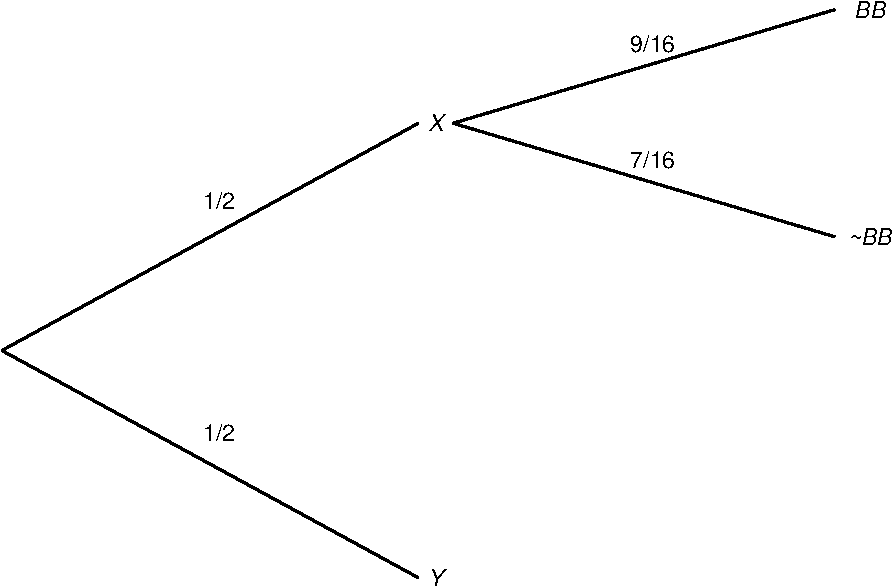
\includegraphics{_main_files/figure-latex/unnamed-chunk-70-1} 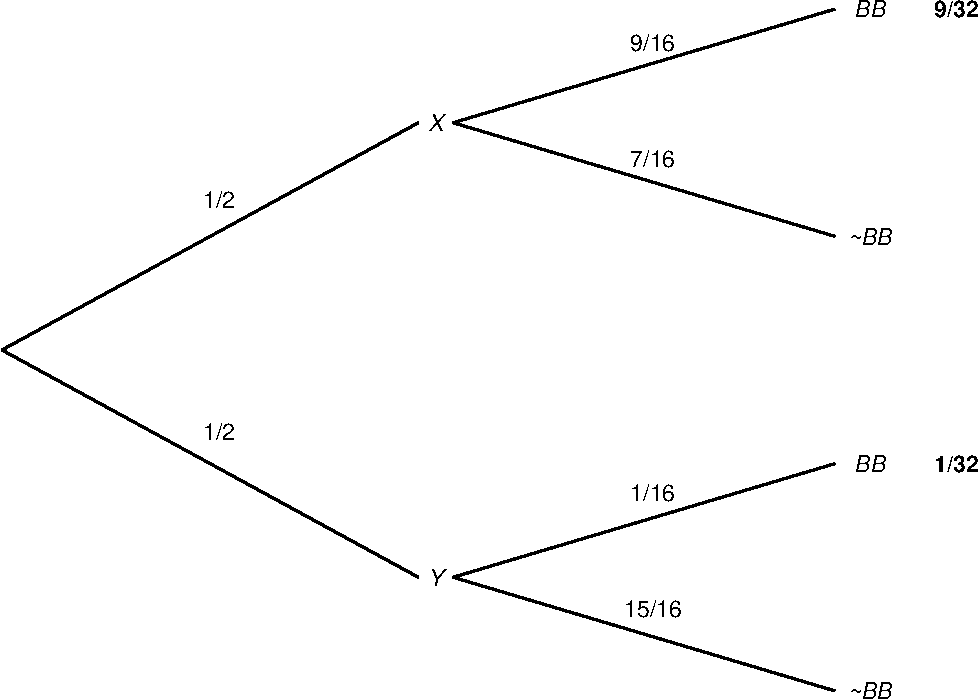
\includegraphics{_main_files/figure-latex/unnamed-chunk-70-2} \caption[Building a probability tree to solve Laplace's urn puzzle]{Building a probability tree to solve Laplace's urn puzzle}\label{fig:unnamed-chunk-70}
\end{marginfigure}

Depending on how the coin lands, you could end up drawing either from
Urn X or from Urn Y, with equal probability.

If you end up drawing from Urn X, the probability of a black marble on
any given draw is \(3/4\). Because the draws are independent (we're
drawing with replacement), the probability they'll both come up black is
\(3/4 \times 3/4 = 9/16\).

If instead you end up drawing from Urn Y, the probability of a black
marble on any given draw is \(1/4\). The draws are still independent
though, so the chance of both being black in this case is
\(1/4 \times 1/4 = 1/16\).

So the probability of drawing two black marbles from Urn X is: \[
  \begin{aligned}
    \p(X \wedge BB) &= \p(X) \p(BB \given X)\\
                    &= 1/2 \times 9/16\\
                    &= 9/32.
  \end{aligned}
\] And the probability of drawing two black marbles from Urn Y is: \[
  \begin{aligned}
    \p(Y \wedge BB) &= \p(Y) \p(BB \given Y)\\
                    &= 1/2 \times 1/16\\
                    &= 1/32.
  \end{aligned}
\] Now we can apply the Addition Rule to calcualte \(\p(BB)\): \[
  \begin{aligned}
    \p(BB) &= \p(X \wedge BB) + \p(Y \wedge BB)\\
           &= 9/32 + 1/32\\
           &= 5/16.
  \end{aligned}
\]

\hypertarget{the-law-of-total-probability}{%
\section{The Law of Total
Probability}\label{the-law-of-total-probability}}

\newthought{This} kind of calculation comes up a lot. Since it would be
tedious to figure it out from scratch every time, we make a general rule
instead:

\begin{description}
\item[The Law of Total Probability]
\(\p(A) = \p(A \given B) \p(B) + \p(A \given \neg B) \p(\neg B)\).
\end{description}

There's an intuitive idea at work here. To figure out how likely \(A\)
is, consider how likely it would be if \(B\) were true, and how likely
it would be if \(B\) were false. Then weight each of those hypothetical
possibilities according to their probabilities.

\begin{marginfigure}
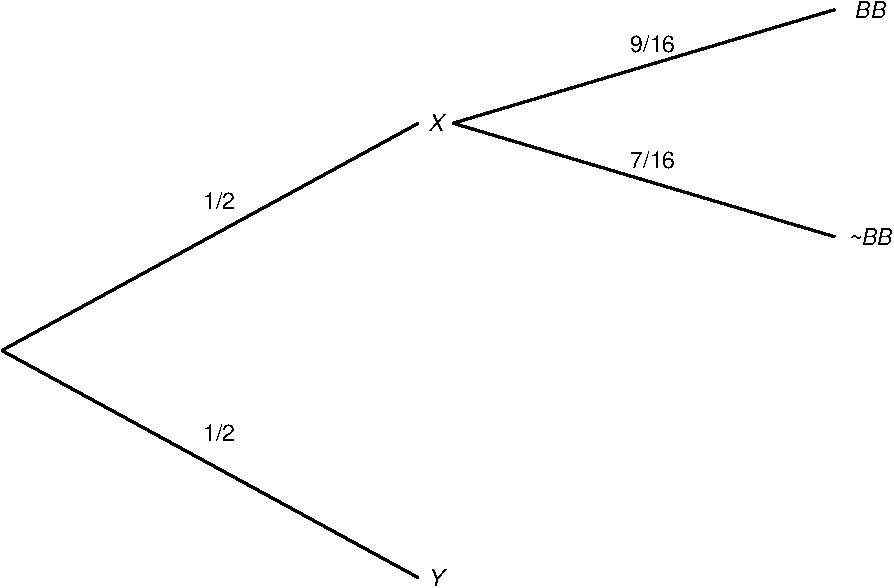
\includegraphics{_main_files/figure-latex/unnamed-chunk-71-1} \caption[The Law of Total Probability calculates the size of the $A$ region by summing its two part]{The Law of Total Probability calculates the size of the $A$ region by summing its two part.}\label{fig:unnamed-chunk-71}
\end{marginfigure}

We can also use an Euler diagram. The size of the \(A\) region is the
sum of the \(A \wedge B\) region and the \(A \wedge \neg B\) region:
\(\color{bookpurple}{\blacksquare}\color{black}{} + \color{bookred}{\blacksquare}\color{black}{}\).
And each of those regions can be calculated using the General
Multiplication Rule. For example,
\(\p(A \wedge B) = \p(A \given B) \p(B)\). So in algebraic terms we
have: \[
  \begin{aligned}
    \p(A) &= \color{bookpurple}{\blacksquare}\color{black}{} 
             + \color{bookred}{\blacksquare}\color{black}{}\\
          &= \p(A \wedge B) + \p(A \wedge \neg B)\\
          &= \p(A \given B) \p(B) + \p(A \given \neg B) \p(\neg B).
  \end{aligned}
\] Which is precisely the Law of Total Probability.

\begin{marginfigure}
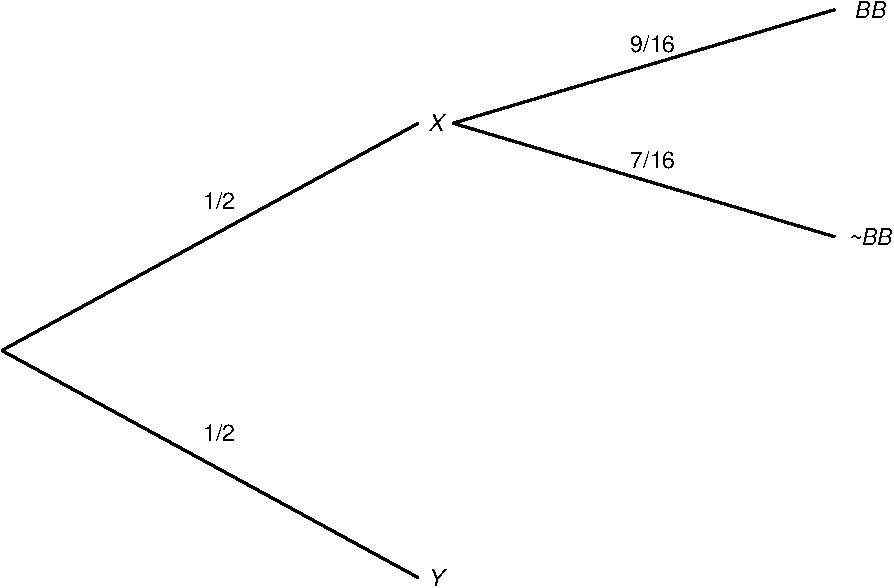
\includegraphics{_main_files/figure-latex/unnamed-chunk-72-1} \caption[The Law of Total Probability in a tree diagram]{The Law of Total Probability in a tree diagram}\label{fig:unnamed-chunk-72}
\end{marginfigure}

We can also use a tree diagram to illustrate the same reasoning. There
are two leaves where \(A\) is true, marked

\includegraphics[width=0.18in]{img/emoji_shades_small} and

\includegraphics[width=0.18in]{img/emoji_hearts_small} . To get the
probability of each leaf we multiply across the branches (that's the
General Multiplication Rule). And then to get the total probability for
\(A\), we add up the two leaves: \(\p(A) =\)\\

\includegraphics[width=0.18in]{img/emoji_shades_small} \(+\)

\includegraphics[width=0.18in]{img/emoji_hearts_small} . Once again the
result is the Law of Total Probability: \[
  \p(A) = \p(A \given B) \p(B) + \p(A \given \neg B) \p(\neg B).
\]

\begin{warning}
Black hole warning: notice that the Law of Total Probability depends on
\(\p(A \given B)\) and \(\p(A \given \neg B)\) both being well-defined.
So it only applies when \(\p(B) \gt 0\) and \(\p(\neg B) \gt 0\).
\end{warning}

\hypertarget{example}{%
\section{Example}\label{example}}

\newthought{Every} day Professor X either drives her car to campus or
takes the bus. Mostly she drives, but one time in four she takes the
bus. When she drives, she's on time \(80\%\) of the time. When she takes
the bus, she's on-time \(90\%\) of the time.

What is the probability she'll be on time for class tomorrow?

First let's solve this by just applying the Law of Total Probability
directly: \[
  \begin{aligned}
    \p(O) &= \p(O \given B)\p(B) + \p(O \given D)\p(D)\\
          &= (9/10)(1/4) + (8/10)(3/4)\\
          &= 33/40.
  \end{aligned}
\]

Now let's solve it slightly differently, thinking the problem through
from more basic principles.

There are two, mutually exclusive cases where Professor X is on time:
one where she takes the bus, one where she drives.
\[ \p(O) = \p(O \wedge B) + \p(O \wedge D). \] We can use the General
Multiplication Rule to calculate the probability she'll take the bus and
be on time: \[ \p(O \wedge B) = \p(O \given B)\p(B). \] And we can do
the same for the probability she'll drive and be on time:
\[ \p(O \wedge D) = \p(O \given D)\p(D)\] Putting all the pieces
together: \[
  \begin{aligned}
    \p(O) &= \p(O \wedge B) + \p(O \wedge D)\\
          &= \p(O \given B)\p(B) + \p(O \given D)\p(D)\\
          &= (9/10)(1/4) + (8/10)(3/4)\\
          &= 33/40.
  \end{aligned}
\]

Notice that we didn't just get the same answer, we ended up doing the
same calculation too. Our second approach just reconstructed from
scratch the reasoning behind the Law of Total Probability. It's a very
good idea to understand the rationale behind the Law of Total
Probability. But once you get used to the formula, it's also fine to
skip straight to applying it directly.

\begin{marginfigure}
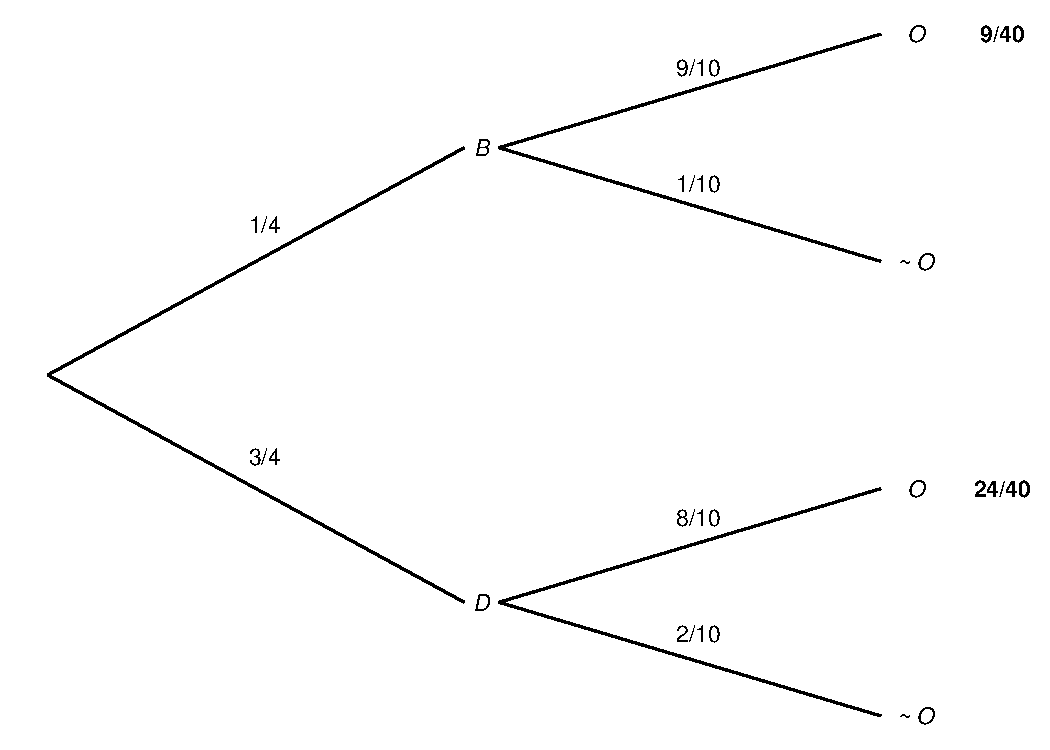
\includegraphics{_main_files/figure-latex/unnamed-chunk-74-5} \caption[A probability tree for Professor X]{A probability tree for Professor X}\label{fig:unnamed-chunk-74}
\end{marginfigure}

You can also use a tree diagram. Again, the calculation will be the
same. But the diagram may help you get started, and it helps you check
that you've applied the formula correctly too.

\hypertarget{exercises-5}{%
\section*{Exercises}\label{exercises-5}}
\addcontentsline{toc}{section}{Exercises}

\begin{enumerate}
\item
  Suppose you have an ordinary deck of \(52\) playing cards, and you
  draw one card at random. What is the probability you will draw:

  \begin{enumerate}
  \def\labelenumii{\alph{enumii}.}
  \tightlist
  \item
    A face card (king, queen, or jack)?
  \item
    A card that is not a face card?
  \item
    An ace or a spade?
  \item
    A queen or a heart?
  \item
    A queen or a non-spade?
  \end{enumerate}
\item
  Suppose that \(Pr(A)=1/3\), \(Pr(B) = 1/4\), and that \(A\) and \(B\)
  are independent. What is \(\p(\neg A \wedge \neg B)\)?
\item
  What is \(\p(X \vee B)\) in the first version of the urn problem? (The
  first version is the one where we start with a fair coin flip to
  choose between Urn X and Urn Y, then draw one marble at random.)
\item
  Recall Laplace's version of the urn puzzle: we select either Urn X or
  Urn Y at random, then we do two random draws from it, with
  replacement. What is \(\p(X \vee BB)\)?
\item
  Suppose we add a third urn to Laplace's puzzle: Urn Z contains \(2\)
  black marbles and \(2\) white ones. We choose one of the three urns at
  random, and then do two random draws with replacement. What is
  \(\p(BB)\) then?
\item
  The Law of Total probability calculates \(\p(A)\) by considering two
  cases, \(B\) and \(\neg B\). Notice that \(B\) and \(\neg B\) form a
  \protect\hyperlink{lessons}{partition}: they are mutually exclusive
  and exhaustive possibilities.

  Suppose we had a partition of three propositions instead: \(B\),
  \(C\), and \(D\). Would the following extension of the Law of Total
  Probability hold then?
  \[\p(A) = \p(A \given B)\p(B) + \p(A \given C)\p(C) + \p(A \given D)\p(D).\]
  Justify your answer.
\item
  Suppose there are two urns with the following contents:

  \begin{itemize}
  \tightlist
  \item
    Urn I has 8 black balls, 2 white.
  \item
    Urn II has 2 black balls, 3 white.
  \end{itemize}

  A fair coin will be flipped. If it comes up heads, a ball will be
  drawn from Urn I at random. Otherwise a ball will be drawn from Urn II
  at random. What is the probability a black ball will be drawn?
\item
  Suppose you have an ordinary deck of 52 cards. A card is drawn and is
  \textbf{not replaced}, then another card is drawn. Assume that on each
  draw all the cards then in the deck have an equal chance of being
  drawn.

  \begin{enumerate}
  \def\labelenumii{\alph{enumii}.}
  \tightlist
  \item
    What is the probability of getting an ace on draw 1?
  \item
    What is the probability of a ten on draw 2 given ace on draw 1?
  \item
    What is the probability of an ace on draw 1 and a ten on draw 2?
  \item
    What is the probability of a ten on draw 1 and an ace on draw 2?
  \item
    What is the probability of an ace and a ten?
  \item
    What is the probability of 2 aces?
  \end{enumerate}
\item
  The probability that George will study for the final is \(4/5\). The
  probability he will pass given that he studies is \(3/5\). The
  probability he will pass given that he does not study is \(1/10\).
  What is the probability George will pass?
\item
  Calculate each of the following probabilities:

  \begin{enumerate}
  \def\labelenumii{\alph{enumii}.}
  \tightlist
  \item
    \(Pr(P) = 1/2\), \(Pr(Q) = 1/2\), \(Pr(P \wedge Q) = 1/8\). What is
    \(Pr(P \vee Q)\)?
  \item
    \(Pr(R) = 1/2, Pr(S) = 1/4, Pr(R \vee S) = 3/4\). What is
    \(Pr(R \wedge S)\)?
  \item
    \(Pr(U) = 1/2, Pr(T) = 3/4, Pr(U \wedge \neg T) = 1/8\). What is
    \(Pr(U \vee \neg T)\)?
  \end{enumerate}
\item
  \(Pr(P) = 1/2, Pr(Q) = 1/2\), and \(P\) and \(Q\) are independent.

  \begin{enumerate}
  \def\labelenumii{\alph{enumii}.}
  \tightlist
  \item
    What is \(Pr(P {\,\&\,}Q)\)?
  \item
    Are \(P\) and \(Q\) mutually exclusive?
  \item
    What is \(Pr(P \vee Q)\)?
  \end{enumerate}
\item
  Suppose \(A\), \(B\), and \(C\) are all mutually exclusive, and they
  each have the same probability: \(1/5\). What is
  \(\p(\neg(A \wedge B) \wedge C)\)?
\item
  Researchers are studying the safety of drug X. They enroll 60 subjects
  in a study and give drug X to 35 of them. By the end of the study, 5
  subjects have developed stomach cancer: 3 who were taking drug X, 2
  who were not.

  Draw a Venn diagram and use it to answer the following questions about
  a randomly selected subject:

  \begin{enumerate}
  \def\labelenumii{\alph{enumii}.}
  \tightlist
  \item
    What is the probability they developed stomach cancer?
  \item
    What is the probability they developed stomach cancer given that
    they were taking drug X?
  \item
    What is the probability they developed stomach cancer given that
    they were not taking drug X?
  \item
    Based on this study, would you conclude that drug X increases or
    decreases the risk of stomach cancer?
  \end{enumerate}
\item
  There is a room filled with two types of urns.

  \begin{itemize}
  \tightlist
  \item
    Type A urns contain 30 yellow marbles, 70 red.
  \item
    Type B urns contain 20 green marbles, 80 yellow.
  \end{itemize}

  The two types of urn look identical, but 80\% of them are Type A.

  \begin{enumerate}
  \def\labelenumii{\alph{enumii}.}
  \tightlist
  \item
    You pick an urn at random and draw a marble from it at random. What
    is the probability the marble will be yellow?
  \item
    You look at the marble: it is yellow. What's the probability the urn
    is a Type B urn?
  \end{enumerate}
\item
  Suppose \(A\), \(B\), and \(C\) are independent of one another. Does
  it follow that \(\p(B \given A \wedge C) = \p(B)\)? Justify your
  answer.
\item
  Is the following combination of probabilities possible?
  \(Pr(A) = 2/5\), \(Pr(B) = 4/5\), and \(Pr(A \vee B) = 3/5\). Justify
  your answer.
\item
  Which of the following situations is impossible? Justify your answer.

  \begin{enumerate}
  \def\labelenumii{\alph{enumii}.}
  \tightlist
  \item
    \(\p(A) = 4/5\), \(\p(B) = 1/5\), \(\p(\neg A \wedge B) = 3/5\).
  \item
    \(\p(\neg X) = 1/3\), \(\p(\neg Y) = 2/3\), \(\p(X \wedge Y) = 0\).
  \end{enumerate}
\item
  If \(Pr(A)=0\), what is \(\p(A \given B)\)? Justify your answer.
\item
  Do Exercise 2 from p.~67 of Hacking.
\item
  Do Exercise 3 from p.~67 of Hacking.
\item
  If \(A\) and \(B\) are logically equivalent, what is
  \(\p(A \given B)\)? Justify your answer.
\item
  Suppose \(A\), \(B\), and \(C\) all have the same probability, namely
  \(1/4\). Suppose they are also independent of one another. What is
  \(\p(\neg A \vee \neg B \vee \neg C)\)?

  Hint: \(\neg A \vee \neg B \vee \neg C\) is logically equivalent to
  \(\neg (A \wedge B \wedge C)\). Why?
\item
  If \(\p(A) = 1/2\) and \(\p(B) = 3/5\), are \(A\) and \(B\) mutually
  exclusive? Justify your answer.
\item
  Suppose \(\p(A) = 1/4\), \(\p(B) = 1/3\), and \(A\) and \(B\) are
  independent. What is \(\p(A \vee (B \wedge \neg A))\)?
\item
  Suppose \(A\) logically entails \(C\), and \(A\) and \(B\) are
  independent. If \(\p(A) = 1/7\), \(\p(B) = 1/3\), and \(\p(C)=1/3\),
  what is \(\p((A \wedge \neg B) \vee \neg C)\)?
\item
  If \(A\) and \(B\) are mutually exclusive, must the following hold?
  \[\p(A \vee B \given C) = \p(A \given C) + \p(B \given C).\] Assume
  the conditional probabilities are all well-defined, and justify your
  answer.

  Hint: apply the definition of conditional probability and use the
  following fact: \((A \vee B) \wedge C\) is logically equivalent to
  \((A \wedge C) \vee (B \wedge C)\).
\item
  Prove that if \(A\) and \(B\) are mutually exclusive, then
  \[\p(A \given A \vee B) = \frac{ \p(A) }{ \p(A) + \p(B) }.\]
\item
  If \(\p(C \given B \wedge A) = \p(C \given B)\), does this follow?
  \[\p(A \given B \wedge C) = Pr(A \given B).\] Assume all conditional
  probabilities are well-defined, and justify your answer.
\item
  Justify the claim from
  \protect\hyperlink{declaring-independence}{Chapter 6} that
  independence extends to negations: if \(A\) is independent of \(B\),
  then it's also independent of \(\neg B\) (provided
  \(\p(\neg A) > 0\)).

  Warning: this one is hard. I suggest starting with the equation:
  \[ \p(A \wedge B) = \p(A) \p(B). \] Then use the Negation Rule which
  tells us: \[ \p(B) = 1 - \p(\neg B). \] And use the Addition Rule to
  get: \[ \p(A \wedge B) = \p(A) - \p(A \wedge \neg B).\]
\end{enumerate}

\hypertarget{chbayes}{%
\chapter{Bayes' Theorem}\label{chbayes}}

\begin{marginfigure}
The experiment was first published in 1971. It was performed by
\href{https://en.wikipedia.org/wiki/Daniel_Kahneman}{Daniel Kahneman}
and \href{https://en.wikipedia.org/wiki/Amos_Tversky}{Amos Tversky}.
Their work on human reasoning reshaped the field of psychology, and
eventually won a Nobel prize in 2002.
\end{marginfigure}

\newthought{In} a famous psychology experiment, subjects were asked to
solve the following problem.

\begin{problem}
A cab was involved in a hit and run accident at night. Two cab
companies, the Green and the Blue, operate in the city. You are given
the following data:

\begin{enumerate}
\def\labelenumi{\arabic{enumi}.}
\tightlist
\item
  \(85\%\) of the cabs in the city are Green and \(15\%\) are Blue.
\item
  A witness identified the cab as Blue. The court tested the reliability
  of the witness under the same circumstances that existed on the night
  of the accident and concluded that the witness correctly identified
  each one of the two colors \(80\%\) of the time and failed \(20\%\) of
  the time.
\end{enumerate}

What is the probability that the cab involved in the accident was blue
rather green?
\end{problem}

Most people answer \(80\%\), because the witness is \(80\%\) reliable.
But the right answer is \(12/29\), or about \(41\%\).

How could the probability be so low when the witness is \(80\%\)
reliable? The short answer is: because blue cabs are rare. So most of
the time, when the witness says a cab is blue, it's one of the \(20\%\)
of green cabs they mistakenly identify as blue.

But this answer still needs some explaining. Let's use a diagram.

\begin{marginfigure}
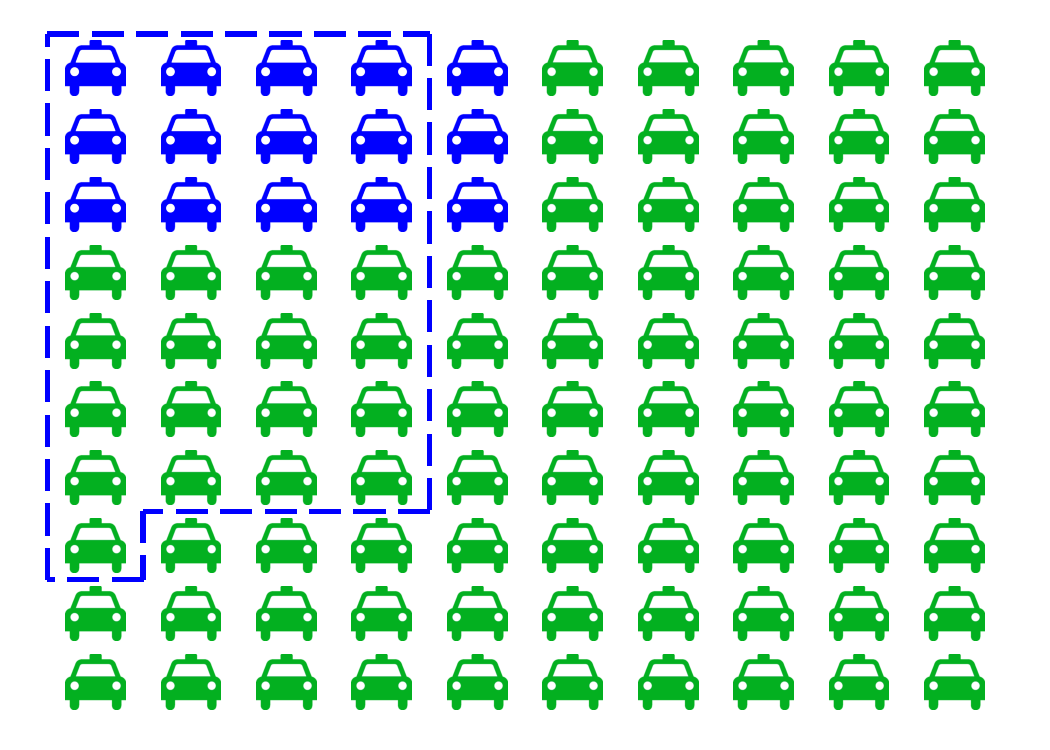
\includegraphics{_main_files/figure-latex/taxigrid-11} \caption[The taxicab problem]{The taxicab problem. There are $15$ blue cabs, $85$ green. The dashed region indicates those cabs the witness identifies as "blue". It includes $80\%$ of the blue cabs ($12$), and only $20\%$ of the green ones ($17$). Yet it includes more green cabs than blue.}\label{fig:taxigrid}
\end{marginfigure}

Imagine there are just \(100\) cabs in town, \(85\) green and \(15\)
blue. The dashed blue line represents the cabs the witness identifies as
``blue'', both right or wrong. Because the witness is \(80\%\) accurate,
that line encompasses \(80\%\) of the blue cabs, which is \(12\) cabs.
But it also encompasses \(20\%\) of the green cabs, which is \(17\).
That's a total of \(29\) cabs identified as ``blue'', only \(12\) of
which actually are blue.

So out of the \(29\) cabs the witness calls ``blue'', only \(12\) really
are blue. The probability a cab really is blue given the witness says so
is only \(12/29\), about \(41\%\).

Another way to think about the problem is that there are \emph{two}
pieces of information relevant to whether the cab is blue. The witness
says the cab is blue, but also, most cabs are not blue. So there's
evidence for the cab being blue, but also strong evidence against it.
The diagram in Figure \ref{fig:taxigrid} shows us how to balance these
two, competing pieces of evidence and come to the correct answer.

What trips people up so much in the taxicab problem? Remember how order
matters with conditional probability. In this problem, we're asked to
find \(\p(B \given W)\), the probability the cab is blue given that the
witness says it is. That's not the same as \(\p(W \given B)\), the
probability the witness will say the cab is blue if it really is. The
problem tells us \(\p(W \given B) = 8/10\), but it doesn't tell us a
number for \(\p(B \given W)\). We have to figure that out.

We saw back in \protect\hyperlink{conditional-probability}{Chapter 6}
that \(\p(A \given B)\) is usually a different number from
\(\p(B \given A)\). A university student will probably be young, but a
young person will probably not be a university student. That's an
example where it's easy to see that order matters. The taxicab example
makes it much less obvious, in fact it tempts us to confuse
\(\p(B \given W)\) with \(\p(W \given B)\).

\hypertarget{bayes-theorem}{%
\section{Bayes' Theorem}\label{bayes-theorem}}

\newthought{Problems} where we're given \(\p(B \given A)\) and we have
to figure out \(\p(A \given B)\) are extremely common. Luckily, there's
a famous formula for solving them.

\begin{marginfigure}
\href{https://en.wikipedia.org/wiki/Thomas_Bayes}{Thomas Bayes}
(1701--1761) was an English minister and mathematician, the first to
formulate the theorem that now bears his name.
\end{marginfigure}

\begin{description}
\item[Bayes' Theorem]
If \(\p(A),\p(B)>0\), then
\[ \p(A \given B) = \frac{\p(A)\p(B \given A)}{\p(B)}. \]
\end{description}

Notice two things here. First, we need \(\p(A)\) and \(\p(B)\) to both
be positive, because otherwise \(\p(A \given B)\) and \(\p(B \given A)\)
aren't well-defined. Second, we need to know more than just
\(\p(B \given A)\) to apply the formula. We also need numbers for
\(\p(A)\) and \(\p(B)\).

In the taxicab problem we're given two of the three pieces of
information we need. Here's Bayes' theorem for the taxicab example:
\[ \p(B \given W) = \frac{\p(B) \p(W \given B)}{\p(W)}. \] Whereas the
problem gives us the following information:

\begin{itemize}
\tightlist
\item
  \(\p(W \given B) = 80/100\).
\item
  \(\p(W \given \neg B) = 20/100\).
\item
  \(\p(B) = 15/100\).
\item
  \(\p(\neg B) = 85/100\).
\end{itemize}

What's missing for Bayes' Theorem is \(\p(W)\). Fortunately, we can
calculate it with the Law of Total Probability! \[
  \begin{aligned}
    \p(W) &= \p(W \given B)\p(B) + \p(W \given \neg B)\p(\neg B)\\
          &= (80/100)(15/100) + (20/100)(85/100)\\
          &= 29/100.
  \end{aligned}
\] And now we have everything we need to plug into Bayes' Theorem: \[
  \begin{aligned}
    \p(B \given W) &= \frac{\p(B) \p(W \given B)}{\p(W)}\\
                   &= \frac{(15/100)(80/100)}{29/100}\\
                   &= 12/29.
  \end{aligned}
\] This is the same answer we got with our grid diagram (Figure
\ref{fig:taxigrid}). And notice, it's also the answer we'd get from a
tree diagram too (Figure \ref{fig:taxitree}).

\begin{marginfigure}
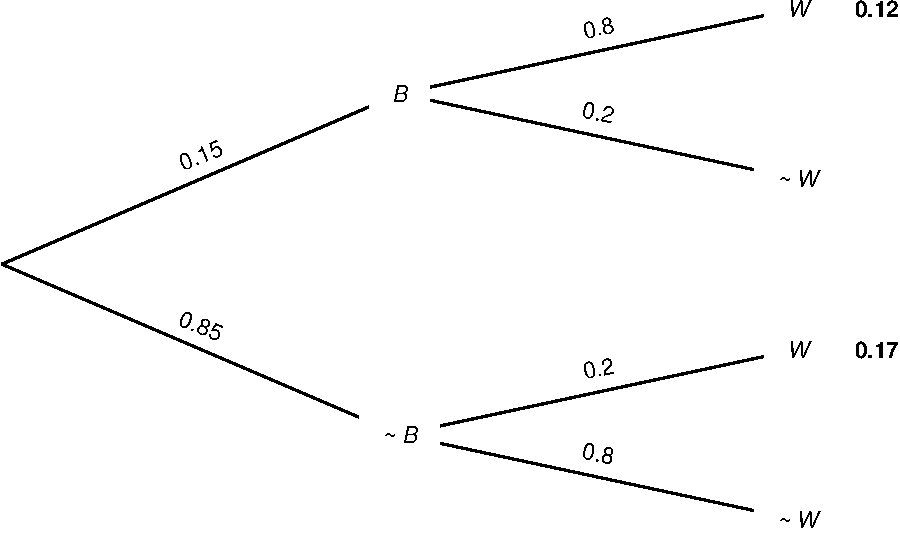
\includegraphics{_main_files/figure-latex/taxitree-1} \caption[Tree diagram for the taxicab problem]{Tree diagram for the taxicab problem. Since $\p(B \wedge W) = .12$ and $\p(W) = .12 + .17$, the definition of conditional probability yields $\p(B \given W) = 12/29$.}\label{fig:taxitree}
\end{marginfigure}

\hypertarget{understanding-bayes-theorem}{%
\section{Understanding Bayes'
Theorem}\label{understanding-bayes-theorem}}

\newthought{Why} does Bayes' theorem work? One way to think about it is
to start by recalling the definition of conditional probability:
\[ \p(A \given B) = \frac{\p(A \wedge B)}{\p(B)}. \] Then apply the
General Multiplication Rule to the numerator:
\[ \p(A \wedge B) = \p(B \given A)\p(A).\] And plug that back into the
first equation:
\[ \p(A \given B) = \frac{\p(A) \p(B \given A)}{\p(B)}. \] This proves
that Bayes' theorem is correct. But it also suggests a way of
understanding it visually, with an Euler diagram.

\begin{marginfigure}
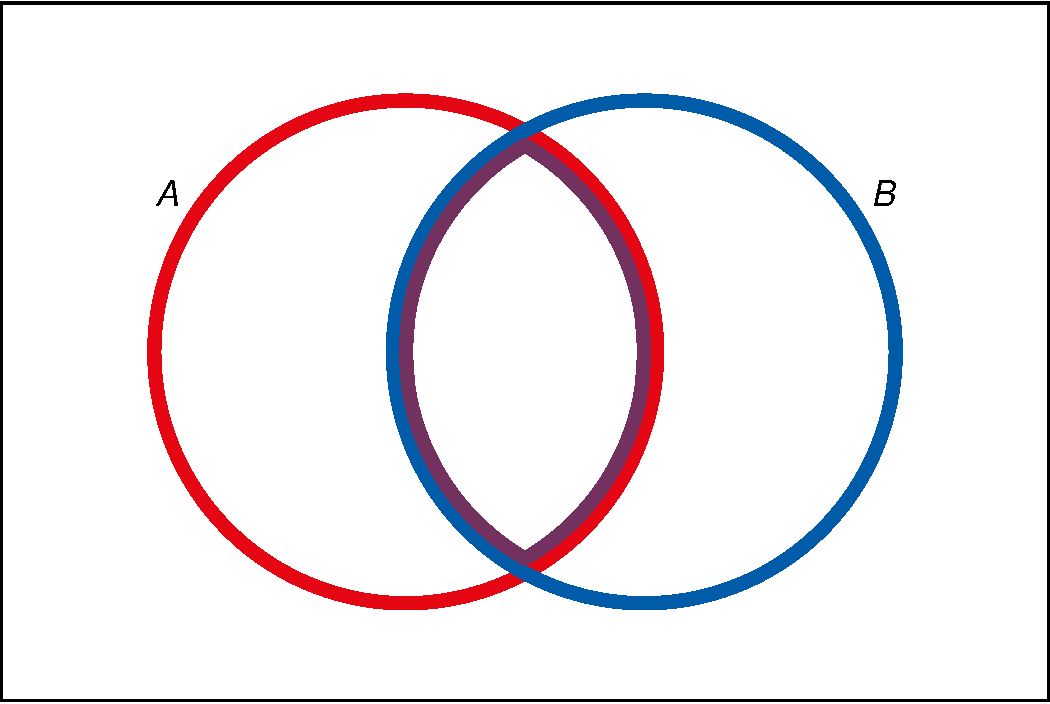
\includegraphics{_main_files/figure-latex/unnamed-chunk-79-1} \caption[An Euler diagram for visualizing Bayes' theorem]{An Euler diagram for visualizing Bayes' theorem}\label{fig:unnamed-chunk-79}
\end{marginfigure}

\newthought{We've talked} before about \(\p(A \given B)\) being the
portion of the \(B\) region that's inside the \(A\) region. The purple
portion of the blue \(B\) circle, in other words: \[
  \begin{aligned}
    \p(A \given B) &= \frac{ \color{bookpurple}{\p(A \wedge B)} }{ \color{bookblue}{\p(B)} }.\\
  \end{aligned}
\] So when we apply the General Multiplication Rule to the purple region
we get: \[
  \begin{aligned}
    \p(A \given B) &= \frac{ \color{bookpurple}{\p(B \given A)\p(A)} }{ \color{bookblue}{\p(B)} }.\\
  \end{aligned}
\]

We'll come back to another, non-visual way of understanding Bayes'
theorem in \protect\hyperlink{bayesibe}{Chapter 10}.

\newthought{There} are lots more visual explanations of Bayes' theorem
you can find online. There's even one
\href{https://www.countbayesie.com/blog/2015/2/18/bayes-theorem-with-lego}{using
Legos}! But they all tend to come down to the same thing. A two step
explanation that goes:

\begin{enumerate}
\def\labelenumi{\arabic{enumi}.}
\tightlist
\item
  Start with the definition of conditional probability, which we learned
  how to visualize in
  \protect\hyperlink{calculating-conditional-probability}{Chapter 6}.
\item
  Then apply the General Multiplication Rule, which we learned how to
  visualize in
  \protect\hyperlink{the-general-multiplication-rule}{Chapter 7}.
\end{enumerate}

This is a perfectly good and helpful way to think about Bayes' theorem.
But it's not really a visualization of the theorem itself. It's two
separate visualizations of the ingredients we use to derive the theorem.

\begin{marginfigure}
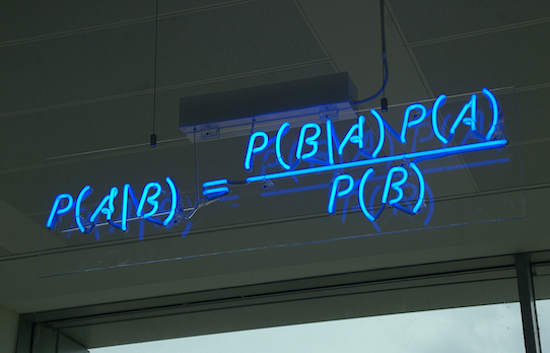
\includegraphics[width=1.83in]{img/neon_bayes} \caption[Bayes' theorem on display at the offices of HP Autonomy, in Cambridge, UK]{Bayes' theorem on display at the offices of HP Autonomy, in Cambridge, UK}\label{fig:neonbayes}
\end{marginfigure}

In any case, Bayes' theorem comes up so often it's good to memorize the
formula itself. The visualization in Figure \ref{fig:neonbayes} is
probably about as helpful as it gets for this purpose.

\hypertarget{bayes-long-theorem}{%
\section{Bayes' Long Theorem}\label{bayes-long-theorem}}

\newthought{We} had to apply the Law of Total Probability first, before
we could solve the taxicab problem with Bayes' theorem, to calculate the
denominator. This is so common that you'll often see Bayes' theorem
written with this calculation built in. That is, the denominator
\(\p(B)\) is expanded out using the Law of Total Probability.

\begin{description}
\item[Bayes' Theorem (long version)]
If \(1 > \p(A) > 0\) and \(\p(B)>0\), then
\[ \p(A \given B) = \frac{\p(A)\p(B \given A)}{\p(A)\p(B \given A) + \p(\neg A)\p(B \given \neg A)}. \]
\end{description}

Notice how there's some repetition in the numerator and the denominator.
The term \(\p(A)\p(B \given A)\) appears both above and below. So, when
you're doing a calculation with this formula, you can just do that bit
once and then copy it in both the top and bottom. Then you just have to
do the bottom-right term to complete the formula.

\begin{marginfigure}
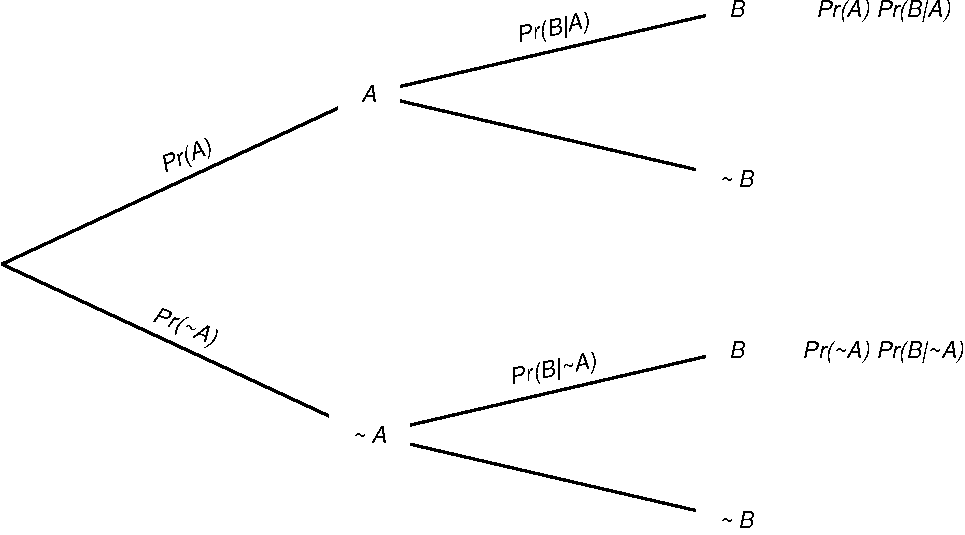
\includegraphics{_main_files/figure-latex/longbayestree-1} \caption[A tree diagram for the long form of Bayes' theorem]{A tree diagram for the long form of Bayes' theorem. The definition of conditional probability tells us $\p(A \given B)$ is the first leaf divided by the sum of the first and third leaves.}\label{fig:longbayestree}
\end{marginfigure}

\newthought{A} tree diagram helps illuminate the long version of Bayes'
theorem. To calculate \(\p(A \given B)\), the definition of conditional
probability directs us to calculate \(\p(A \wedge B)\) and \(\p(B)\):
\[ \p(A \given B) = \frac{ \p(A \wedge B) }{ \p(B) }. \] Looking at the
tree diagram in Figure \ref{fig:longbayestree}, we see that this amounts
to computing the first leaf for the numerator, and the sum of the first
and third leaves for the denominator. Which yields the same formula as
in the long form of Bayes' theorem.

\hypertarget{example-1}{%
\section{Example}\label{example-1}}

\newthought{Let's} practice the long form of Bayes' theorem.

\begin{problem}
Joe has just heard about the Zika virus and wonders if he has it. His
doctor tells him only \(1\%\) of the population has the virus, but he's
still worried. There's a blood test he can take, but it's not perfect.
The test always comes up either negative or positive, but:

\begin{itemize}
\tightlist
\item
  95\% of people who have the virus test positive.
\item
  85\% of people who don't have the virus test negative.
\end{itemize}

If Joe tests positive, what is the probability he really has the Zika
virus?
\end{problem}

We're asked to calculate \(\p(Z \given P)\), and we're given the
following:

\begin{itemize}
\tightlist
\item
  \(\p(Z) = 1/100\).
\item
  \(\p(P \given Z) = 95/100\).
\item
  \(\p(P \given \neg Z) = 15/100\).
\end{itemize}

So we can calculate \(\p(Z \given P)\) using the long form of Bayes'
theorem: \[
  \begin{aligned}
    \p(Z \given P) &= \frac{\p(Z)\p(P \given Z)}{\p(Z)\p(P \given Z) + \p(\neg Z)\p(P \given \neg Z)}\\
                   &= \frac{(1/100)(95/100)}{(1/100)(95/100) + (99/100)(15/100)}\\
                   &= \frac{95}{95 + 1,485}\\
                   &= 19/316\\
                   &\approx .06.
  \end{aligned}
\] The calculation is also diagrammed in Figure \ref{fig:zikatree}.

\begin{marginfigure}
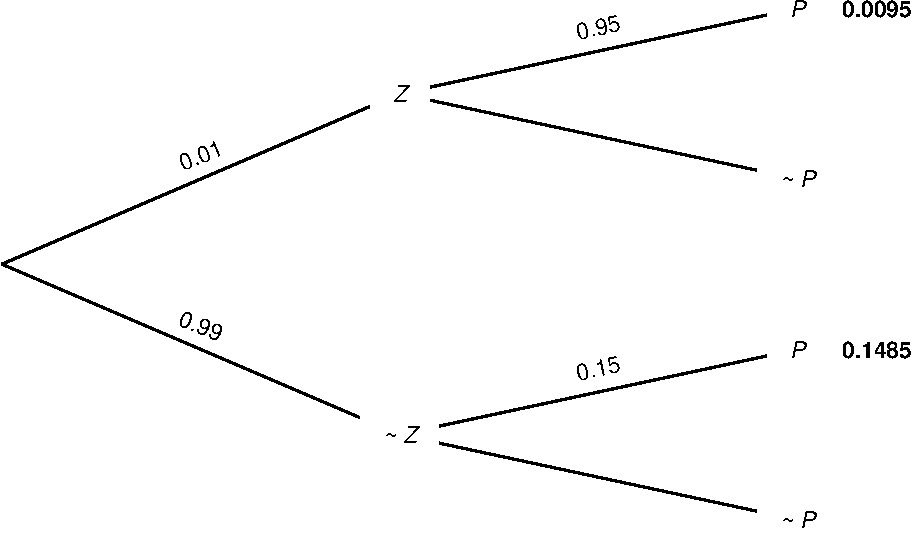
\includegraphics{_main_files/figure-latex/zikatree-1} \caption[Tree diagram of the Zika problem]{Tree diagram of the Zika problem}\label{fig:zikatree}
\end{marginfigure}

It turns out there's only about a \(6\%\) chance Joe has the virus. Even
though he tested positive with a fairly reliable blood test! It's
counterintuitive, but the reason is the same as with the taxicab
problem. There are two, conflicting pieces of evidence: the blood test
is positive but the virus is rare. It turns out the virus is so rare
that the positive blood test doesn't do much to increase Joe's chances
of being infected.

\newthought{Bayes' theorem} doesn't always give such surprising results.
In fact the results are often very intuitive. Professors just like to
use the counterintuitive examples to demonstrate how important Bayes'
theorem is. Without it, it's easy to go astray.

\hypertarget{baserate}{%
\section{The Base Rate Fallacy}\label{baserate}}

\newthought{In} the Zika example, the rate of infection in the general
population is very low, just \(1\%\). The rate at which something
happens in general is called the \emph{base rate}. In the taxicab
example, the base rate for blue cabs was \(15\%\).

One lesson of this chapter is that you have to take the base rate into
account to get the right answer, via Bayes' theorem. Humans have a
tendency to ignore the base rate, and focus only on the ``test''
performed: the blood test in the Zika example, the testimony of the
witness in the taxicab example. This mistake is called \emph{base rate
neglect}, or \emph{the base rate fallacy}.

The base rate fallacy is so tempting, even trained professionals are
susceptible to it. In
\href{https://www.stat.berkeley.edu/~aldous/157/Papers/health_stats.pdf}{one
famous study}, \(160\) medical doctors were given a problem similar to
our Zika example (but with cancer instead of Zika). The question was
multiple choice, and it used easier numbers than we did. Yet only \(34\)
of the doctors got it right.

Hence the quote that opens
\protect\hyperlink{the-monty-hall-problem}{Chapter 1} of this book: ``in
no other branch of mathematics is it so easy for experts to blunder as
in probability theory.''

\hypertarget{exercises-6}{%
\section*{Exercises}\label{exercises-6}}
\addcontentsline{toc}{section}{Exercises}

\begin{enumerate}
\item
  Recall this problem from \protect\hyperlink{ch6ex}{Chapter 6}:

  \begin{quote}
  Five percent of tablets made by the company Ixian have factory
  defects. Ten percent of the tablets made by their competitor company
  Guild do. A computer store buys \(40\%\) of its tablets from Ixian,
  and \(60\%\) from Guild.
  \end{quote}

  Use Bayes' theorem to find \(\p(I \given D)\), the probability a
  tablet from this store is made by Ixian, given that it has a factory
  defect?
\item
  Recall this problem from \protect\hyperlink{ch6ex}{Chapter 6}:

  \begin{quote}
  In the city of Elizabeth, the neighbourhood of Southside has lots of
  chemical plants. \(2\%\) of Elizabeth's children live in Southside,
  and \(14\%\) of those children have been exposed to toxic levels of
  lead. Elsewhere in the city, only \(1\%\) of the children have toxic
  levels of exposure.
  \end{quote}

  Use Bayes' theorem to find \(\p(S \given L)\), the probability that a
  randomly chosen child from Elizabeth who has toxic levels of lead
  exposure lives in Southside?
\item
  The probability that Nasim will study for her test is \(4/10\). The
  probability that she will pass, given that she studies, is \(9/10\).
  The probability that she passes, given that she does not study, is
  \(3/10\). What is the probability that she has studied, given that she
  passes?
\item
  At the height of flu season, roughly \(1\) in every \(100\) people
  have the flu. But some people don't show symptoms even when they have
  it: only half the people who have the virus show symptoms.

  Flu symptoms can also be caused by other things, like colds and
  allergies. So about \(1\) in every \(20\) people who don't have the
  flu still have flu-like symptoms.

  If someone has flu-like symptoms at the height of flu season, what is
  the probability that they actually have the flu?
\item
  A magic shop sells two kinds of trick coins. The first kind are biased
  towards heads: they come up heads \(9\) times out of \(10\) (the
  tosses are independent). The second kind are biased towards tails:
  they comes up tails \(8\) times out of \(10\) (tosses still
  independent). Half the coins are the first kind, half are the second
  kind. But they don't label the coins, so you have to experiment to
  find out which are which.

  You pick a coin at random and flip it once. Given that it comes up
  heads, what is the probability it's the first kind of coin?
\item
  There is a room filled with two types of urns.

  \begin{itemize}
  \tightlist
  \item
    Type A urns have \(30\) yellow marbles, \(70\) red.
  \item
    Type B urns have \(20\) green marbles, \(80\) yellow.
  \end{itemize}

  The two types of urn look identical, but \(80\%\) of them are Type A.
  You pick an urn at random and draw a marble from it at random.

  \begin{enumerate}
  \def\labelenumii{\alph{enumii}.}
  \tightlist
  \item
    What is the probability the marble will be yellow?
  \end{enumerate}

  Now you look at the marble: it is yellow.

  \begin{enumerate}
  \def\labelenumii{\alph{enumii}.}
  \setcounter{enumii}{1}
  \tightlist
  \item
    What is the probability the urn is a Type B urn, given that you drew
    a yellow marble?
  \end{enumerate}
\item
  In the long form of Bayes' theorem, the denominator is broken down by
  applying the Law of Total Probability to a partition of two
  propositions, \(A\) and \(\neg A\). We can extend the same idea to a
  partition of three propositions, \(X\), \(Y\), and \(Z\). Here is a
  start on the formula:

  \[ \p(X \given B) = \frac{\p(X)\p(B \given X)}{\p(X)\p(B \given X) + \;\ldots\;}.\]

  Fill in the rest of the formula, then justify it.
\item
  A company makes websites, always powered by one of three server
  platforms: Bulldozer, Kumquat, or Penguin. Bulldozer crashes \(1\) out
  of every \(10\) visits, Kumquat crashes \(1\) in \(50\) visits, and
  Penguin only crashes \(1\) out of every \(200\) visits.

  \begin{marginfigure}
  This problem is based on Exercise 6 from p.~78 of Ian Hacking's \emph{An
  Introduction to Probability \& Inductive Logic}.
  \end{marginfigure}

  Half of the websites are run on Bulldozer, \(30\%\) are run on
  Kumquat, and \(20\%\) are run on Penguin.

  You visit one of their sites for the first time and it crashes. What
  is the probability it was run on Penguin?
\item
  You and Carlos are at a party, which means there's a \(2/3\) chance
  he's been drinking. You decide to experiment to find out: you throw a
  tennis ball to Carlos and he misses the catch. Five minutes later you
  try again and he misses again. Assume the two catches are independent.

  When he's sober, Carlos misses a catch only two times out of ten. When
  he's been drinking, Carlos misses catches half the time.

  What is the probability that Carlos has been drinking, given that he
  missed both catches?
\item
  The Queen Gertrude Hotel has two kinds of suites: singles have one
  bed, royal suites have three beds. There are \(80\) singles and \(20\)
  royals.

  In a single, the probability of bed bugs is \(1/100\). But every
  additional bed put in a suite doubles the chance of bed bugs.

  If a suite is inspected at random and bed bugs are found, what is the
  probability it's a royal?
\item
  Willy Wonka Chocolates Inc.~makes two kinds of boxes of chocolates.
  The ``wonk box'' has four caramel chocolates and six regular
  chocolates. The ``zonk box'' has six caramel chocolates, two regular
  chocolates, and two mint chocolates. A third of their boxes are wonk
  boxes, the rest are zonk boxes.

  They don't mark the boxes. The only way to tell what kind of box
  you've bought is by trying the chocolates inside. In fact, all the
  chocolates look the same; you can only tell the difference by tasting
  them.

  If you buy a random box, try a chocolate at random, and find that it's
  caramel, what is the probability you've bought a wonk box?
\item
  A room contains four urns. Three of them are Type X, one is Type Y.

  \begin{itemize}
  \tightlist
  \item
    The Type X urns each contain \(3\) black marbles, \(2\) white
    marbles.
  \item
    The Type Y urn contains \(1\) black marble, \(4\) white marbles.
  \end{itemize}

  You are going to pick an urn at random and start drawing marbles from
  it at random \emph{without} replacement.

  What is the probability the urn is Type X if the first draw is black?
\end{enumerate}

\hypertarget{multiple-conditions}{%
\chapter{Multiple Conditions}\label{multiple-conditions}}

\newthought{We} often need to account for multiple pieces of evidence.
More than one witness testifies about the colour of a taxicab; more than
one person responds to our poll about an upcoming election; etc.

How do we a calculate conditional probability when there are multiple
conditions? In other words, how do we handle quantities of the form
\(\p(A \given B_1 \wedge B_2 \wedge \ldots)\)?

\hypertarget{multiple-draws}{%
\section{Multiple Draws}\label{multiple-draws}}

\newthought{Imagine} you're faced with another one of our mystery urns.
There are two equally likely possibilities: \[
  \begin{aligned}
    A      &: \mbox{The urn contains $70$ black marbles, $30$ white marbles.}\\
    \neg A &: \mbox{The urn contains $20$ black marbles, $80$ white marbles.}\\
  \end{aligned}
\] Now suppose you draw a marble at random and it's black. You put it
back, give the urn a good shake, and then draw another: black again.
What's the probability the urn has \(70\) black marbles?

We need to calculate \(\p(A \given B_1 \wedge B_2)\), the probability of
\(A\) given that the first and second draws were both black. We already
know how to do this calculation for one draw, \(\p(A \given B_1)\). We
use Bayes' theorem to get: \[
  \begin{aligned}
    \p(A \given B_1) &= \frac{\p(B_1 \given A)\p(A)}{\p(B_1 \given A) \p(A) + \p(B_1 \given \neg A) \p(\neg A)} \\
      &= \frac{(70/100)(1/2)}{(70/100)(1/2) + (20/100)(1/2)}\\
      &= 7/9.
  \end{aligned}
\]

But for two draws, Bayes' theorem gives us: \[
  \begin{aligned}
    \p(A \given B_1 \wedge B_2) &= \frac{\p(B_1 \wedge B_2 \given A)\p(A)}{\p(B_1 \wedge B_2 \given A) \p(A) + \p(B_1 \wedge B_2 \given \neg A) \p(\neg A)}.
  \end{aligned}
\] To fill in the values on the right hand side, we need to know these
quantities:

\begin{itemize}
\tightlist
\item
  \(\p(B_1 \wedge B_2 \given A)\),
\item
  \(\p(B_1 \wedge B_2 \given \neg A)\).
\end{itemize}

To get the first quantity, remember that we replaced the first marble
before doing the second draw. So, given \(A\), the second draw is
independent of the first. There are still \(70\) black marbles out of
\(100\) on the second draw, so the chance of black on the second draw is
still \(70/100\). In other words: \[
  \begin{aligned}
    \p(B_1 \wedge B_2 \given A) &= \p(B_1 \given A) \p(B_2 \given A)\\
      &= (70/100)^2.
  \end{aligned}
\] The same reasoning applies given \(\neg A\), too. Except here the
chance of black on each draw is \(20/100\). So: \[
  \begin{aligned}
    \p(B_1 \wedge B_2 \given \neg A) &= \p(B_1 \given \neg A) \p(B_2 \given \neg A)\\
      &= (20/100)^2.
  \end{aligned}
\]

Returning to Bayes' theorem, we can now finish the calculation: \[
  \begin{aligned}
    \p(A \given B_1 \wedge B_2) &= \frac{\p(B_1 \wedge B_2 \given A)\p(A)}{\p(B_1 \wedge B_2 \given A) \p(A) + \p(B_1 \wedge B_2 \given \neg A) \p(\neg A)} \\ 
    &= \frac{(70/100)^2(1/2)}{(70/100)^2(1/2) + (20/100)^2(1/2)}\\
    &= 49/53.
  \end{aligned}
\]

\newthought{The} same solution can also be captured in a probability
tree. The tree will have an extra stage now, because there's a second
draw. And it will have many more leaves, but luckily we can ignore most
of them. We just need to worry about the two leaves where both draws
have come up black. And we only need to fill in the probabilities along
the paths that lead to those two leaves. The result is Figure
\ref{fig:twodrawsreplacement}.

\begin{figure}
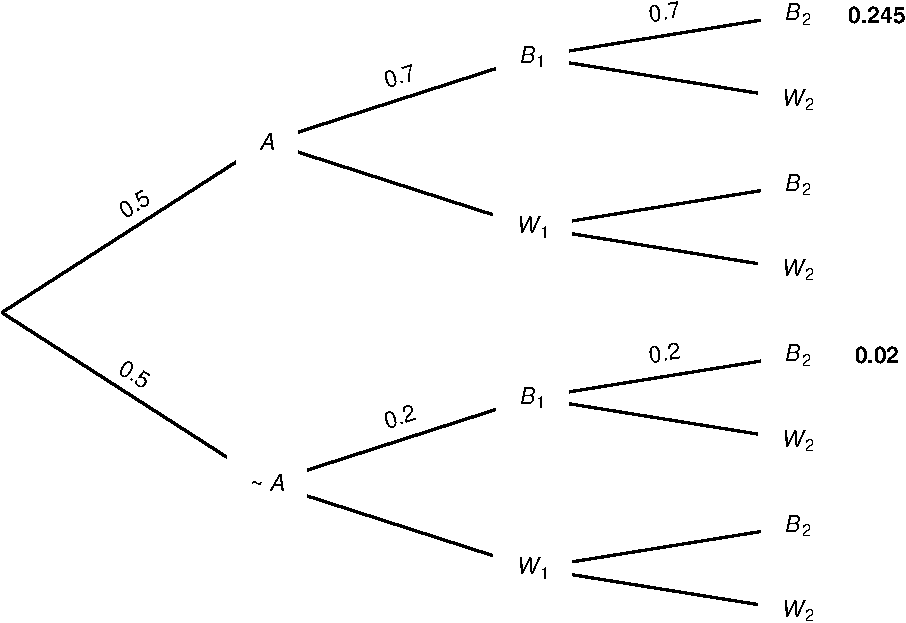
\includegraphics{_main_files/figure-latex/twodrawsreplacement-1} \caption[Tree diagram for two draws with replacement]{Tree diagram for two draws with replacement}\label{fig:twodrawsreplacement}
\end{figure}

So \(\p(A \given B_1 \wedge B_2) = 0.245 / (0.245 + 0.2)\), which is the
same as \(49/53\), the answer we got with Bayes' theorem.

\newthought{You} might be able to guess now what would happen after
three black draws. Instead of getting squared probabilities in Bayes'
theorem, we'd get cubed probabilities. And using the same logic, we
could keep going. We could use Bayes' theorem to calculate
\(\p(A \given B_1 \wedge \ldots \wedge B_n)\) for as many draws \(n\) as
you like.

\hypertarget{multiple-witnesses}{%
\section{Multiple Witnesses}\label{multiple-witnesses}}

\newthought{Let's try} a different sort of problem with multiple
conditions. Recall the taxicab problem from
\protect\hyperlink{chbayes}{Chapter 8}:

\BeginKnitrBlock{problem}
A cab was involved in a hit and run accident at night. Two cab
companies, the Green and the Blue, operate in the city. You are given
the following data:

\begin{enumerate}
\def\labelenumi{\arabic{enumi}.}
\tightlist
\item
  \(85\%\) of the cabs in the city are Green and \(15\%\) are Blue.
\item
  A witness identified the cab as Blue. The court tested the reliability
  of the witness under the same circumstances that existed on the night
  of the accident and concluded that the witness correctly identified
  each one of the two colors \(80\%\) of the time and failed \(20\%\) of
  the time.
\end{enumerate}

What is the probability that the cab involved in the accident was blue
rather green?
\EndKnitrBlock{problem}

We saw it's only about \(41\%\) likely the cab was really blue, even
with the witness' testimony. But what if there had been two witnesses,
both saying the cab was blue?

Let's use Bayes' theorem again: \[
  \begin{aligned}
    \p(B \given W_1 \wedge W_2) &= \frac{\p(B)\p(W_1 \wedge W_2 \given B)}{\p(W_1 \wedge W_2)}.
  \end{aligned}
\] We have one of the terms here already: \(\p(B) = 15/100\). What about
the other two:

\begin{itemize}
\tightlist
\item
  \(\p(W_1 \wedge W_2 \given B)\),
\item
  \(\p(W_1 \wedge W_2)\).
\end{itemize}

Let's make things easy on ourselves by assuming our two witnesses are
reporting independently. They don't talk to each other, or influence one
another in any way. They're only reporting what they saw (or think they
saw). Then we can ``factor'' these probabilities like we did when
sampling with replacement: \[
  \begin{aligned}
    \p(W_1 \wedge W_2 \given B) &= \p(W_1 \given B) \p(W_2 \given B)\\
                                &= (80/100)^2.
  \end{aligned}
\] And for the denominator we use the Law of Total Probability: \[
  \begin{aligned}
    \p(W_1 \wedge W_2) &= \p(W_1 \wedge W_2 \given B)\p(B) + 
                          \p(W_1 \wedge W_2 \given \neg B)\p(\neg B)\\
                       &= (80/100)^2(15/100) + (20/100)^2(85/100)\\
                       &= 96/1000 + 34/1000\\
                       &= 13/100.
  \end{aligned}
\]

Now we can return to Bayes' theorem to finish the problem: \[
  \begin{aligned}
    \p(B \given W_1 \wedge W_2) &= \frac{(15/100)(80/100)^2}{13/100}\\
                                &= 96/130\\
                                &\approx .74.
  \end{aligned}
\] So, with two witnesses independently agreeing that the cab was blue,
the probability goes up from less than \(1/2\) to almost \(3/4\).

\begin{marginfigure}
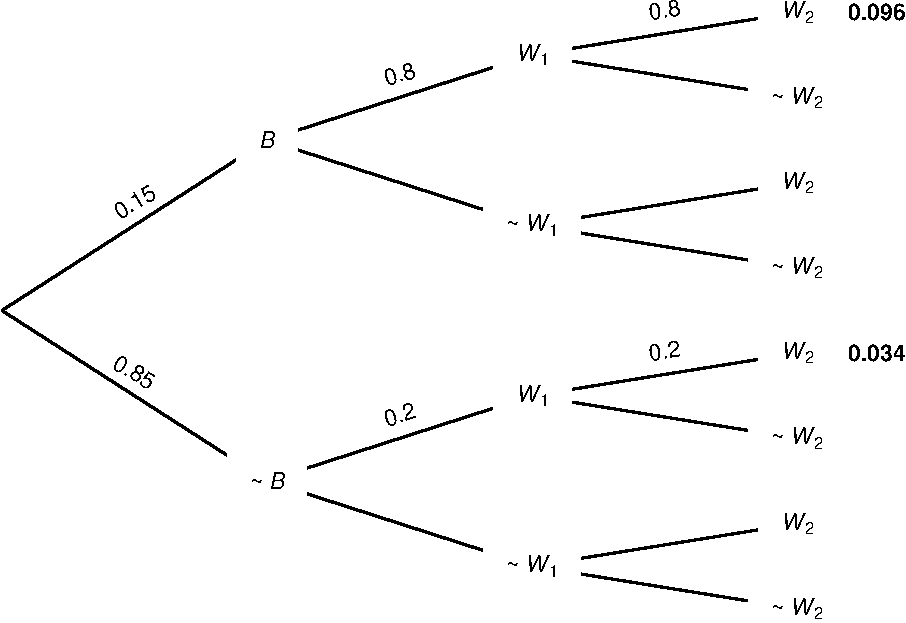
\includegraphics{_main_files/figure-latex/twowitnesstree-1} \caption[Tree diagram for the two-witness taxicab problem]{Tree diagram for the two-witness taxicab problem}\label{fig:twowitnesstree}
\end{marginfigure}

\newthought{We} can use a tree here too, similar to the one we made when
sampling two black marbles with replacement. As before, we only need to
worry about the \(W_1 \wedge W_2\) leaves, the ones where both witnesses
say the cab was blue. The result is Figure \ref{fig:twowitnesstree},
which tells us that
\(\p(B \given W_1 \wedge W_2) = 0.096 / (0.096 + 0.034)\), which is
approximately \(0.74\).

\hypertarget{without-replacement}{%
\section{Without Replacement}\label{without-replacement}}

\newthought{The} problems we've done so far were simplified by assuming
independence. We sampled with replacement in the urn problem, and we
assumed our two witnesses were independently reporting what they saw in
the taxicab problem. What about when independence doesn't hold?

Let's go back to our urn problem, but this time suppose we don't replace
the marble after the first draw. How do we calculate
\(\p(A \given B_1 \wedge B_2)\) then?

We're still going to start with Bayes' theorem: \[
  \begin{aligned}
    \p(A \given B_1 \wedge B_2) &= \frac{\p(B_1 \wedge B_2 \given A)\p(A)}{\p(B_1 \wedge B_2 \given A) \p(A) + \p(B_1 \wedge B_2 \given \neg A) \p(\neg A)}.
  \end{aligned}
\] But to calculate terms like \(\p(B_1 \wedge B_2 \given A)\) now, we
need to think things through in two steps.

We know the first draw has a \(70/100\) chance of coming up black if
\(A\) is true: \[ \p(B_1 \given A) = 70/100. \] And once the first draw
has come up black, if \(A\) is true then there are 69 black balls
remaining and 30 white. So: \[ \p(B_2 \given B_1 \wedge A) = 69/99. \]
So instead of multiplying \(70/100\) by itself, we're multiplying
\(70/100\) by \emph{almost} \(70/100\): \[
  \begin{aligned}
    \p(B_1 \wedge B_2 \given A) &= (70/100)(69/99)\\
       &= 161/300.
  \end{aligned}
\]

Using similar reasoning for the possibility that \(\neg A\) instead, we
can calculate \[
  \begin{aligned}
    \p(B_1 \wedge B_2 \given \neg A) &= (20/100)(19/99)\\
       &= 19/495.
  \end{aligned}
\]

Returning to Bayes' theorem to finish the calculation: \[
  \begin{aligned}
    \p(A \given B_1 \wedge B_2) &= \frac{\p(B_1 \wedge B_2 \given A)\p(A)}{\p(B_1 \wedge B_2 \given A) \p(A) + \p(B_1 \wedge B_2 \given \neg A) \p(\neg A)} \\
      &= \frac{(161/300)(1/2)}{(161/300)(1/2) + (19/495)(1/2)} \\
      &= 5313/5693 \\
      &\approx .93. 
  \end{aligned}
\] Notice how similar this answer is to the \(.92\) we got when sampling
with replacement. With so many black and white marbles in the urn,
taking one out doesn't make much difference. The second draw is almost
the same as the first, so the final answer isn't much affected.

\begin{marginfigure}
\includegraphics{_main_files/figure-latex/twodrawsnoreplacement-1} \caption[Tree diagram for two draws with replacement, values rounded]{Tree diagram for two draws with replacement, values rounded}\label{fig:twodrawsnoreplacement}
\end{marginfigure}

\newthought{The} tree diagram for this problem will also be similar to
the with-replacement version. The key difference is the probabilities at
the last stage of the tree. Without independence, the probability of a
\(B_2\) branch is affected by the \(B_1\) that precedes it. The result
is Figure \ref{fig:twodrawsnoreplacement}, though note that some values
are rounded. Still we find that: \[
  \begin{aligned}
     \p(A \given B_1 \wedge B_2) &\approx \frac{ 0.2439 }{ 0.2439 + 0.0192 } \\
                                 &\approx 0.93.
  \end{aligned}
\]

\hypertarget{multiplying-conditional-probabilities}{%
\section{Multiplying Conditional
Probabilities}\label{multiplying-conditional-probabilities}}

\newthought{The} calculation we just did relied on a new rule, which we
should make explicit. Start by recalling a familiar rule:

\begin{description}
\item[The General Multiplication Rule]
\(\p(A \wedge B) = \p(A \given B) \p(B).\)
\end{description}

Our new rule applies the same idea to situations where some proposition
\(C\) is taken as a given.

\begin{description}
\item[The General Multiplication Rule (Conditional Version)]
\(\p(A \wedge B \given C) = \p(A \given B \wedge C) \p(B \given C).\)
\end{description}

In a way, the new rule isn't really new. We just have to realize that
the probabilities we get when we take a condition \(C\) as given are
still probabilities. They obey all the same rules as unconditional
probabilities, and this includes the General Multiplication Rule.

Another example which illustrates this point is the Negation Rule. The
following conditional version is also valid:

\begin{description}
\item[The Negation Rule (Conditional Version)]
\(\p(\neg A \given C) = 1 - \p(A \given C).\)
\end{description}

We could go through all the rules of probability we've learned and write
out the conditional version for each one. But we've already got enough
rules and equations to keep track of. So let's just remember this mantra
instead:

\begin{info}
Conditional probabilities are probabilities.
\end{info}

So if we have a rule of probability, the same rule will hold if we add a
condition \(C\) into each of the \(\p(\ldots)\) terms.

\hypertarget{summary-2}{%
\section{Summary}\label{summary-2}}

\newthought{We've learned two strategies} for calculating conditional
probabilities with multiple conditions.

The first strategy is easier, but it only works when the conditions are
appropriately independent. Like when we sample with replacement, or when
two witnesses independently report what they saw.

In this kind of case, we first use Bayes' theorem, and then ``factor''
the terms: \[
  \begin{aligned}
    \p(A \given B_1 \wedge B_2) &= 
      \frac{\p(B_1 \wedge B_2 \given A)\p(A)}{%
            \p(B_1 \wedge B_2 \given A)\p(A) +%
              \p(B_1 \wedge B_2 \given \neg A)\p(\neg A)}\\
      &= \frac{\p(B_1 \given A)\p(B_2 \given A)\p(A)}{%
                \p(B_1 \given A)\p(B_2 \given A)\p(A) +%
                  \p(B_1 \given \neg A)\p(B_2 \given \neg A)\p(\neg A)}\\
      &= \frac{(\p(B_1 \given A))^2\p(A)}{%
                (\p(B_1 \given A))^2\p(A) +%
                  (\p(B_1 \given \neg A))^2\p(\neg A)}.
  \end{aligned}
\]

Our second strategy is a little more difficult. But it works even when
the conditions are \textbf{not} independent. We still start with Bayes'
theorem. But then we apply the conditional form of the General
Multiplication Rule: \[
  \begin{aligned}
    \p(A \given B_1 \wedge B_2) &= 
      \frac{\p(B_1 \wedge B_2 \given A)\p(A)}{%
            \p(B_1 \wedge B_2 \given A)\p(A) +%
              \p(B_1 \wedge B_2 \given \neg A)\p(\neg A)}\\
      &= \frac{\p(B_2 \given B_1 \wedge A)\p(B_1 \given A)\p(A)}{%
                \p(B_2 \given B_1 \wedge A)\p(B_1 \given A)\p(A) +%
                  \p(B_2 \given B_1 \wedge \neg A)\p(B_1 \given \neg A)\p(\neg A)}.
  \end{aligned}
\]

These are some pretty hairy formulas, so memorizing them probably isn't
a good idea. It's better to understand how they flow from Bayes' theorem
or a tree diagram.

\hypertarget{exercises-7}{%
\section*{Exercises}\label{exercises-7}}
\addcontentsline{toc}{section}{Exercises}

\begin{enumerate}
\item
  Recall the following problem from
  \protect\hyperlink{bayes-theorem}{Chapter 8}.

  Willy Wonka Co.~makes two kinds of boxes of chocolates. The ``wonk
  box'' has four caramel chocolates and six regular chocolates. The
  ``zonk box'' has six caramel chocolates, two regular chocolates, and
  two mint chocolates. A third of their boxes are wonk boxes, the rest
  are zonk boxes.

  They don't mark the boxes. The only way to tell what kind of box
  you've bought is by trying the chocolates inside. In fact, all the
  chocolates look the same; you can only tell the difference by tasting
  them.

  Previously you calculated the probability a randomly chosen box is a
  wonk box given that a chocolate randomly selected from it is caramel.
  This time, suppose you randomly select two chocolates.

  \begin{enumerate}
  \def\labelenumii{\alph{enumii}.}
  \tightlist
  \item
    What is the probability it's a wonk box given that both chocolates
    are caramel?
  \item
    What is the probability it's a wonk box given that the first is
    caramel and the second is regular?
  \item
    What is the probability it's a wonk box given that the first is
    regular and the second is caramel?
  \end{enumerate}
\item
  Recall the following problem from
  \protect\hyperlink{bayes-theorem}{Chapter 8}.

  A magic shop sells two kinds of trick coins. The first kind are biased
  towards heads: they come up heads \(9\) times out of \(10\) (the
  tosses are independent). The second kind are biased towards tails:
  they comes up tails \(8\) times out of \(10\) (tosses still
  independent). Half the coins are the first kind, half are the second
  kind. But they don't label the coins, so you have to experiment to
  find out which are which.

  Previously, you picked a coin at random and flipped it once. But now
  suppose you flip it a second time. What's the probability it's the
  first kind of coin if it lands heads both times?
\item
  Recall the following problem from
  \protect\hyperlink{bayes-theorem}{Chapter 8}.

  There is a room filled with two types of urns.

  \begin{itemize}
  \tightlist
  \item
    Type A urns have \(30\) yellow marbles, \(70\) red.
  \item
    Type B urns have \(20\) green marbles, \(80\) yellow.
  \end{itemize}

  The two types of urn look identical, but \(80\%\) of them are Type A.

  Previously you calculated the probability a randomly selected urn is
  Type B given that one marble randomly drawn from it is yellow. Suppose
  now you put the yellow marble back, shake hard, and draw another
  marble at random from the same urn.

  \begin{enumerate}
  \def\labelenumii{\alph{enumii}.}
  \tightlist
  \item
    If this marble is also yellow, what is the probability the urn is a
    Type B urn?
  \item
    If this marble is instead green, what is the probability the urn is
    a Type B urn?
  \end{enumerate}
\item
  Recall the following problem from
  \protect\hyperlink{bayes-theorem}{Chapter 8}.

  A room contains four urns. Three of them are Type X, one is Type Y.

  \begin{itemize}
  \tightlist
  \item
    The Type X urns each contain \(3\) black marbles, \(2\) white
    marbles.
  \item
    The Type Y urn contains \(1\) black marble, \(4\) white marbles.
  \end{itemize}

  You are going to pick an urn at random and start drawing marbles from
  it at random \emph{without} replacement.

  Previously you calculated the probability the urn is Type X given that
  the first draw is black.

  \begin{enumerate}
  \def\labelenumii{\alph{enumii}.}
  \tightlist
  \item
    What is the probability the urn is Type X if the first draw is black
    and the second is white?
  \item
    What is the probability the urn is Type X if the first draw is white
    and the second is black?
  \item
    What is the probability the third draw will be black, if the first
    draw is black and the second is white?
  \end{enumerate}
\item
  The order in which conditions are given doesn't matter. More
  precisely, the following equation always holds:

  \[ \p(A \given B \wedge C) = \p(A \given C \wedge B).\]

  Use the rules of probability to prove that it always holds.
\item
  The order in which things happen often matters. If the light was red
  but is now green, the intersection is probably safe to drive through.
  But if the light was green and is now red, it's probably not safe.

  We just saw, though, that the order in which conditions are given
  doesn't make any difference to the probability.

  Explain why these two observations do not conflict.
\item
  Above we observed that \(\p(\neg A \given C) = 1 - \p(A \given C)\).
  Prove that this equation holds. Hint: start with the definition of
  conditional probability, and then recall that \(1 = \p(C) / \p(C)\).
\end{enumerate}

\hypertarget{probability-induction}{%
\chapter{Probability \& Induction}\label{probability-induction}}

\newthought{We} met some common types of inductive argument back in
\protect\hyperlink{indargs}{Chapter 2}. Now that we know how to work
with probability, let's use what we've learned to sharpen our
understanding of how those arguments work.

\hypertarget{generalizing-from-observed-instances}{%
\section{Generalizing from Observed
Instances}\label{generalizing-from-observed-instances}}

\newthought{Generalizing} from observed instances was the first major
form of inductive argument we encountered. Suppose you want to know what
colour a particular species of bird tends to be. Then you might go out
and look at a bunch of examples:

\begin{argument}
I've seen \(10\) ravens and they've all been black.\\
Therefore, all ravens are black.
\end{argument}

How strong is this argument?

Observing ravens is a lot like sampling from an urn. Each raven is a
marble, and the population of all ravens is the urn. We don't know what
nature's urn contains at first: it might contain only black ravens, or
it might contain ravens of other colours too. To assess the argument's
strength, we have to calculate
\(\p(A \given B_1 \wedge B_2 \wedge \ldots \wedge B_{10})\): the
probability that all ravens in nature's urn are black, given that the
first raven we observed was black, and the second, and so on, up to the
tenth raven.

We learned how to solve simple problems of this form in the
\protect\hyperlink{multiple-draws}{previous chapter}. For example,
imagine you face another of our mystery urns, and this time there are
two equally likely possibilities: \[
  \begin{aligned}
    A      &: \mbox{The urn contains only black marbles.} \\
    \neg A &: \mbox{The urn contains an equal mix of black and white marbles.} \\
  \end{aligned}
\] If we do two random draws with replacement, and both are black, we
calculate \(\p(A \given B_1 \wedge B_2)\) using Bayes' theorem: \[
  \begin{aligned}
    \p(A \given B_1 \wedge B_2) &= \frac{\p(B_1 \wedge B_2 \given A)\p(A)}{\p(B_1 \wedge B_2 \given A) \p(A) + \p(B_1 \wedge B_2 \given \neg A) \p(\neg A)} \\ 
    &= \frac{(1)^2(1/2)}{(1)^2(1/2) + (1/2)^2(1/2)}\\
    &= 4/5.
  \end{aligned}
\] If we do a third draw with replacement, and it too comes up black, we
replace the squares with cubes. On the fourth draw we'd raise to the
fourth power. And so on. When we get to the tenth black draw, the
calculation becomes: \[
  \begin{aligned}
    \p(A \given B_1 \wedge B_2) &= \frac{(1)^{10}(1/2)}{(1)^{10}(1/2) + (1/2)^{10}(1/2)}\\
    &= 1,024/1,025\\
    &\approx .999.
  \end{aligned}
\] So after ten black draws, we can be about \(99.9\%\) certain the urn
contains only black marbles.

But that doesn't mean our argument that all ravens are black is
\(99.9\%\) strong!

\hypertarget{real-life-is-more-complicated}{%
\section{Real Life Is More
Complicated}\label{real-life-is-more-complicated}}

\newthought{There} are two major limitations to our urn analogy.

\newthought{The} first limitation is that the ravens we observe in real
life aren't randomly sampled from nature's ``urn''. We only observe
ravens in certain locations, for example. But our solution to the urn
problem relied on random sampling. For example, we assumed
\(\p(B_1 \given \neg A) = 1/2\) because the black marbles are just as
likely to be drawn as the white ones, if there are any white ones.

If there are white ravens in the world though, they might be limited to
certain locales.\footnote{In fact there are white ravens,
  \href{https://vancouversun.com/news/local-news/rare-white-raven-spotted-on-vancouver-island}{especially
  in one area of Vancouver Island}.} So the fact we're only observing
ravens in our part of the world could make a big difference to what we
find. It matters whether your sample really is random.

\newthought{The} second limitation is that we pretended there were only
two possibilities: either all the marbles in the urn are black, or half
of them are. And, accordingly, we assumed there was already a 1/2 chance
all the marbles are black, before we even looked at any of them.

In real life though, when we encounter a new species, it could be that
\(90\%\) of them are black, or \(31\%\), or \(42.718\%\), or any portion
from \(0\%\) to \(100\%\). So there are many, many more possibilities.
The possibility that \emph{all} members of the new species (\(100\%\))
are black is just one of these many possibilities. So it would start
with a much lower probability than \(1/2\).

\begin{marginfigure}
In a famous calculation, \protect\hyperlink{fig:laplace}{Laplace} showed
how to solve the second problem. The result was his famous
\href{https://en.wikipedia.org/wiki/Rule_of_succession}{rule of
succession}: if you do \(n\) random draws and they're all black, the
probability the next draw will be black is \((n+1)/(n+2)\).

Laplace's calculation is too advanced for this book. But statistician
Joe Blitzstein gives a nice explanation in
\href{https://www.youtube.com/watch?v=N8O6zd6vTZ8\&list=EC2SOU6wwxB0uwwH80KTQ6ht66KWxbzTIo}{this
video}, for students who have more background in probability
(specifically random variables and probability density functions).
\end{marginfigure}

\newthought{We} could make our analysis more realistic by taking these
complications into account. But the calculations would get ugly, and
we'd have to use calculus to solve the problem. This is the kind of
technical topic you'd cover in a math or statistics class on
probability. But it's not the kind thing this book is about.

For our purposes, the key ideas that matter are as follows. First, the
strength of an inductive argument is a question of conditional
probability: how probable is the argument's conclusion given its
premises? Second, an argument that generalizes from observed instances
is similar to an urn problem, where we guess the contents of the urn by
repeated sampling. And third, we know how to solve simple versions of
these urn problems using Bayes' theorem. In principle, we could also
solve more complicated and realistic versions using the same fundamental
ideas, the math would just be harder.

\hypertarget{bayesibe}{%
\section{Inference to the Best Explanation}\label{bayesibe}}

\newthought{Another} common form of inductive argument we met in
\protect\hyperlink{logic}{Chapter 2} was Inference to the Best
Explanation. An example:

\begin{argument}
My car won't start and the gas gauge reads `empty'.\\
Therefore, my car is out of gas.
\end{argument}

My car being out of gas is a very good explanation of the facts that it
won't start and the gauge reads `empty'. So this seems like a pretty
strong argument.

How do we understand its strength using probability? This is actually a
controversial topic, currently being studied by researchers. There are
different, competing theories about how Inference to the Best
Explanation fits into probability theory. So we'll just look at one,
popular way of understanding things.

Let's start by thinking about what makes an explanation a good one.

\newthought{A} good explanation should account for all the things we're
trying to explain. For example, if we're trying to explain why my car
won't start and the gauge reads `empty', I'd be skeptical if my mechanic
said it's because the brakes are broken. That doesn't account for any of
the symptoms! I'd also be skeptical if they said the gas gauge was
broken. That might fit okay with one of the symptoms (the gauge reads
`empty'), but it doesn't account for the fact the car won't start.

The explanation that my car is out of gas, however, fits both symptoms.
It would account for both the `empty' reading on the gauge and the car's
refusal to start.

A good explanation should also fit with other things I know. For
example, suppose my mechanic tries to explain my car troubles by saying
that both the gauge and the ignition broke down at the same time. But I
know my car is new, it's a highly reliable model, and it was recently
serviced. So my mechanic's explanation doesn't fit well with the other
things I know. It's not a very good explanation.

We have two criteria now for a good explanation:

\begin{enumerate}
\def\labelenumi{\arabic{enumi}.}
\tightlist
\item
  it should account for all the things we're trying to explain, and
\item
  it should fit well with other things we know.
\end{enumerate}

These criteria match up with terms in Bayes' theorem. Imagine we have
some evidence \(E\) we're trying to explain, and some hypothesis \(H\)
that's meant to explain it. Bayes' theorem says:
\[ \p(H \given E) = \frac{\p(H)\p(E \given H)}{\p(E)}. \] How probable
is our explanation \(H\) given our evidence \(E\)? Well, the larger the
terms in the numerator are, the higher that probability is. And the
terms in the numerator correspond to our two criteria for a good
explanation.

\begin{enumerate}
\def\labelenumi{\arabic{enumi}.}
\item
  \(\p(E \given H)\) corresponds to how well our hypothesis \(H\)
  accounts for our evidence \(E\). If \(H\) is the hypothesis that the
  car is out of gas, then \(\p(E \given H) \approx 1\). After all, if
  there's no gas in the car, it's virtually guaranteed that it won't
  start and the gauge will read `empty'. (It's not perfectly guaranteed
  because the gauge could be broken after all, though that's not very
  likely.)
\item
  \(\p(H)\) corresponds to how well our hypothesis fits with other
  things we know. For example, suppose I know it's been a while since I
  put gas in the car. If \(H\) is the hypothesis that the car is out of
  gas, this fits well with what I already know, so \(\p(H)\) will be
  pretty high.

  Whereas if \(H\) is the hypothesis that the gauge and the ignition
  both broke down at the same time, this hypothesis starts out pretty
  improbable given what else I know (it's a new car, a reliable model,
  and recently serviced). So in that case, \(\p(H)\) would be low
\end{enumerate}

So the better \(H\) accounts for the evidence, the larger
\(\p(E \given H)\) will be. And the better \(H\) fits with my background
information, the larger \(\p(H)\) will be. Thus, the better \(H\) is as
an explanation, the larger \(\p(H \given E)\) will be. And thus the
stronger \(E\) will be as an argument for \(H\).

What about the last term in Bayes' theorem though, the denominator
\(\p(E)\)? It corresponds to a virtue of good explanations too!









\begin{marginfigure}
\includegraphics[width=2.12in]{img/moon} \caption[The hammer/feather experiment was performed on the moon
in 1971. See the \href{https://bit.ly/1KLQzOB}{full video here}.]{The hammer/feather experiment was performed on the moon
in 1971. See the \href{https://bit.ly/1KLQzOB}{full video here}.}\label{fig:unnamed-chunk-87}
\end{marginfigure}
\begin{marginfigure}
\includegraphics[width=2in]{img/vacuum} \caption[It's also been performed in vacuum chambers here on
earth. A beautifully filmed example is
\href{https://bit.ly/10hw8mP}{available on YouTube}, courtesy of the
BBC.]{It's also been performed in vacuum chambers here on
earth. A beautifully filmed example is
\href{https://bit.ly/10hw8mP}{available on YouTube}, courtesy of the
BBC.}\label{fig:unnamed-chunk-87}
\end{marginfigure}

Scientists love theories that explain the unexplained. For example,
Newton's theory of physics is able to explain why a heavy object and a
light object, like a hammer and feather, fall to the ground at the same
speed as long as there's no air resistance. If you'd never performed
this experiment before, you'd probably expect the hammer to fall faster.
You'd be surprised to find that the hammer and feather actually hit the
ground at the same time. That Newton's theory explains this surprising
fact strongly supports his theory.

So the ability to explain surprising facts is a third virtue of a good
explanation. And this virtue corresponds to our third term in Bayes'
theorem:

\begin{enumerate}
\def\labelenumi{\arabic{enumi}.}
\setcounter{enumi}{2}
\tightlist
\item
  \(\p(E)\) corresponds to how surprising the evidence \(E\) is. If
  \(E\) is surprising, then \(\p(E)\) will be low, since \(E\) isn't
  something we expect to be true.
\end{enumerate}

And since \(\p(E)\) is in the denominator of Bayes' theorem, a smaller
number there means a \emph{bigger} value for \(\p(H \given E)\). So the
more surprising the finding \(E\) is, the more it supports a hypothesis
\(H\) that explains it.

According to this analysis then, each term in Bayes' theorem corresponds
to a virtue of a good explanation. And that's why Inference to the Best
Explanation works as a form of inductive inference.

\hypertarget{part-part-ii}{%
\part*{Part II}\label{part-part-ii}}
\addcontentsline{toc}{part}{Part II}

\hypertarget{expected-value}{%
\chapter{Expected Value}\label{expected-value}}

\newthought{We've been thinking a lot} about what conclusions our
evidence supports. But a lot of reasoning is \emph{practical}: it's not
just about what to believe, but about what you should \emph{do}. Once
you know how likely the various possible outcomes of a decision are, how
do you make your choice?

\begin{problem}
Suppose you have a free ticket to play one game at the local casino. You
can choose either the Coin Game or the Die Game.

\begin{itemize}
\tightlist
\item
  Coin Game: a fair coin is flipped. You win \(\$1\) if it lands heads,
  nothing otherwise.
\item
  Die Game: a fair die is rolled. You win \(\$3\) if it lands five or
  six, nothing otherwise.
\end{itemize}

Which game should you play?
\end{problem}

The Coin Game has better odds: a \(1/2\) chance of winning vs.~just
\(1/3\) in the Die Game. But the Die Game promises a bigger payoff:
\(\$3\) rather than just \(\$1\). So there are conflicting arguments
here. The odds favour the first choice, while the potential payoffs
favour the second. How do you reconcile these considerations and come to
a decision?

Well, let's think about what would happen in the long run if you played
each game over and over.

Suppose you played the Coin Game over and over, a hundred times. Half
the time you'd win \(\$1\), and half the time you'd win nothing. So
after a hundred plays, you'd probably win about \(\$50\), which is an
average of \(\$0.50\) per play.

Now suppose you played the Die Game a hundred times instead. A third of
the time you'd win \(\$3\), and the other two thirds of the time you'd
win nothing. So after a hundred plays you'd have won about \(\$100\), an
average of about \(\$1\) per play.

In technical terms, this means the Die Game has a higher \emph{expected
value}. In the long run, you'd expect to win about \(\$1\) per play in
the Die Game, as opposed to \(\$0.50\) for the Coin Game.

So the Die Game is the more advantageous one, on this analysis. On
average, people tend to win more playing that game.

\hypertarget{expected-monetary-values}{%
\section{Expected Monetary Values}\label{expected-monetary-values}}

\newthought{To} calculate the expected value of an option, we multiply
each payoff by its probability, and then sum up the results. For
example, our analysis of the Coin Game can be written this way: \[
  \begin{aligned}
    \p(\$1) \times \$1 + \p(\$0) \times \$0 &= (1/2)(\$1) + (1/2)(\$0)\\
      &= \$0.50.
  \end{aligned}
\] And for the Die Game: \[
  \begin{aligned}
    \p(\$3) \times \$3 + \p(\$0) \times \$0 &= (1/3)(\$3) + (2/3)(\$0)\\
      &= \$1.
  \end{aligned}
\]

Sometimes a gamble has the potential to lose money, so we use a negative
number for the ``payoff''. For example, suppose the Die Game is modified
so that you have to pay \(\$3\) if the die lands \(1, 2, 3\), or \(4\).
Then we calculate: \[
  \begin{aligned}
    \p(\$3) \times \$3 + \p(-\$3) \times -\$3 &= (1/3)(\$3) + (2/3)(-\$3)\\
      &= -\$1.
  \end{aligned}
\]

In general, the formula for a game with possible payoffs \(\$x\) and
\(\$y\) is: \[ \p(\$x) \times \$x + \p(\$y) \times \$y. \]

Notice that expected values aren't necessarily what you might think from
the name. The expected value of a game isn't necessarily the amount you
expect to win playing it. If you play the Die Game, you'll either win
\(\$3\) or nothing. But the expected value is \(\$1\). So you actually
know for certain ahead of time that you won't win the expected value,
\(\$1\).

\begin{warning}
The expected value isn't the amount you expect to win from a game. It's
the amount you expect to win \emph{on average, in the long run}, if you
play the game over and over.
\end{warning}

\hypertarget{visualizing-expectations}{%
\section{Visualizing Expectations}\label{visualizing-expectations}}

\newthought{We} can visualize these long run averages as the area in a
diagram. Figure \ref{fig:gambleviz} shows a gamble with a \(1/3\) chance
of paying \(\$2\), and a \(2/3\) chance of paying \(\$6\).

\begin{figure}
\includegraphics{_main_files/figure-latex/gambleviz-1} \caption[A gamble with a $1/3$ chance of paying $\$2$, and a $2/3$ chance of paying $\$6$]{A gamble with a $1/3$ chance of paying $\$2$, and a $2/3$ chance of paying $\$6$}\label{fig:gambleviz}
\end{figure}
\begin{marginfigure}
\includegraphics{_main_files/figure-latex/coindiegame-1} \includegraphics{_main_files/figure-latex/coindiegame-2} \caption[The Coin Game (top) and the Die Game (bottom)]{The Coin Game (top) and the Die Game (bottom)}\label{fig:coindiegame}
\end{marginfigure}

There are two rectangular regions, one for each possible outcome. The
width of each rectangle is the probability of the corresponding outcome,
and the height is the payoff. So each rectangle's area is one term in
the expected value's sum: \[ 1/3 \times \$2 + 2/3 \times \$6. \] The
expected value is thus the area of the two rectangles together, i.e.~the
area of the blue region (about \(\$4.67\) in this example).

The Coin Game and the Die Game are visualized in Figure
\ref{fig:coindiegame}.

\newthought{We} started this chapter wondering how to reconcile
conflicting arguments. The Coin Game has better odds, but the Die Game
has a greater potential payoff.

Well, a rectangle's area can be enlarged by increasing either its width
or its height. Likewise, a payoff's contribution to expected value can
be increased either by increasing its amount or by increasing its
probability.

So the expected value formula answers our opening question by giving
equal weight to the two competing factors. Width (probability) and
height (payoff) are treated the same: neither one is given greater
weight. We just multiply one against the other and take the total area
that results.

\begin{marginfigure}
\includegraphics{_main_files/figure-latex/unnamed-chunk-90-1} \caption[A gamble with one negative payoff, one positive]{A gamble with one negative payoff, one positive}\label{fig:unnamed-chunk-90}
\end{marginfigure}

\newthought{Sometimes} a decision loses money. We use negative dollar
amounts to represent losses. For example, imagine the Coin Game is
modified so that you lose \(\$2\) if the coin lands tails. Then the
expected value is: \[ 1/2 \times \$1 + 1/2 \times -\$2 = -\$1/2.\]

In our diagrams, potential losses extend below the \(x\)-axis. And we
colour them red as a reminder that they are to be subtracted from the
area above the \(x\)-axis. To get the expected value, we subtract the
red area from the blue area.

\hypertarget{more-than-two-outcomes}{%
\section{More Than Two Outcomes}\label{more-than-two-outcomes}}

\newthought{Most} casino games have mor than two possible payoffs. For
that matter, most decisions in life have more than two possible
outcomes. If you buy insurance for your phone, it could end up saving
you \(\$0\), or it could save you \(\$100\), or it might save you
\(\$150\), etc.

So the official definition of expected monetary value is:

\begin{description}
\item[Expected Monetary Value]
Given an act \(A\) with possible consequences
\(\$x_1, \$x_2, \ldots, \$x_n\), the \emph{expected monetary value} of
\(A\) is: \[
  \begin{aligned}
\E(A) &= \p(\$x_1) \times \$x_1 + \p(\$x_2) \times \$x_2 + \ldots + \p(\$x_n) \times \$x_n.
  \end{aligned}
\]
\end{description}

\begin{marginfigure}
\includegraphics{_main_files/figure-latex/unnamed-chunk-91-1} \caption[A gamble with three possible outcomes]{A gamble with three possible outcomes}\label{fig:unnamed-chunk-91}
\end{marginfigure}

For example, suppose a fair die will be rolled and you will win \$1 if
it lands on a low number, \$2 if it's a middling number. If it's a high
number, you lose \$3. Then: \[
  \begin{aligned}
    \E(A) &= (1/3)(\$1) + (1/3)(\$2) + (1/3)(-\$3)\\
          &= \$1/3 + \$2/3 - \$1\\
          &= \$0.
  \end{aligned}
\]

Gambles with more than two outcomes are visualized the same as before.
We just use three or more reactangles, one for each possible outcome.

\hypertarget{fair-prices}{%
\section{Fair Prices}\label{fair-prices}}

\newthought{Imagine} a variation of the Coin Game, where you win \(\$1\)
if the coin lands heads, and you pay \(\$1\) if it lands tails. You
might be able to guess, the expected value of this game is \(\$0\): \[
  \begin{aligned}
    \p(\$1) \times \$1 + \p(-\$1) \times -\$1 &= (1/2)(\$1) + (1/2)(-\$1)\\
      &= 0.
  \end{aligned}
\] If you played over and over again, you'd break even in the long run.
Half the time you'd win a dollar, and the other half of the time you'd
pay a dollar back.

So if someone asked you to pay in order to play this game, that would
seem unfair. Why pay to play if you don't expect to win?

But for a game like the Die Game, asking people to pay to play does seem
fair. In the long run, the casino is going to lose an average of \(\$1\)
per play. So it's only fair that they ask people to pay \(\$1\) to play
that game. In the long run they'll break even. (Of course, a real casino
will demand more so they can turn a profit.)

In general, a game's fair price is thought to be its expected value. If
the expected value is \(\$3\), it's fair to pay \(\$3\) to play. If the
expected value is \(-\$3\), it's fair to ``pay'' \(-\$3\) to play.
Meaning \emph{they should pay you} \(\$3\) to play.

\newthought{Notice} that the expected value of paying the fair price is
always \(\$0\). Suppose you pay \(\$1\) to play the original Die Game,
for example. Because \$1 is automatically deducted from your winnings,
the possible consequences are now \(\$3 - \$1 = \$2\) or
\(\$0 - \$1 = -\$1\). So the expected value of paying \$1 to play is: \[
  \begin{aligned}
    (1/3)(\$2) + (2/3)(-\$1) &= \$2/3 - \$2/3\\
      &= \$0.
  \end{aligned}
\]

That makes sense: if it's a fair price, you shouldn't have any advantage
over the casino. You don't stand to gain or lose money in the long run,
if you pay the fair price to play over and over.

The casino is in the same position. For them, the losses and gains are
reversed: a roll of five or six loses them \$3, and otherwise they lose
nothing. So if you pay them \(\$1\) to play, they either lose \(\$2\) in
the end or gain \(\$1\): \[
  \begin{aligned}
    (1/3)(-\$2) + (2/3)(\$1) &= -\$2/3 + \$2/3\\
      &= \$0.
  \end{aligned}
\]

Since nobody has an advantage, it's a fair deal.

\hypertarget{other-goods}{%
\section{Other Goods}\label{other-goods}}

\newthought{Money} isn't everything, of course. People value lots of
other things, like their health, their family and friends, and their
free time. The concept of expected value can be applied to other goods
besides money, as long as they're quantifiable.

\begin{problem}
Imagine you're taking a trip to Ottawa and you can either drive or go by
train. If you take the train, it's pretty predictable: it's always a
five or six hour ride, with equal probability. If you drive, it's less
predictable. Nine times out of ten it's just a four hour drive. But one
time in ten, an accident causes a traffic jam and it ends up being a ten
hour drive.
\end{problem}

\begin{marginfigure}
\includegraphics{_main_files/figure-latex/unnamed-chunk-93-1} \includegraphics{_main_files/figure-latex/unnamed-chunk-93-2} \caption[Take the train to Ottawa or drive?]{Take the train to Ottawa or drive?}\label{fig:unnamed-chunk-93}
\end{marginfigure}

If all you care about is spending as little time on the road as
possible, should you take the train or drive? \[
  \begin{aligned}
    \E(\mbox{Train}) &= \p(-5{\mbox{ hr}}) \times -5{\mbox{ hr}}+ \p(-6{\mbox{ hr}}) \times -6{\mbox{ hr}}\\
                     &= (1/2)(-5{\mbox{ hr}}) + (1/2)(-6{\mbox{ hr}})\\
                     &= -11/2{\mbox{ hr}}\\
                     &= -5.5{\mbox{ hr}},\\
    \E(\mbox{Drive}) &= \p(-4{\mbox{ hr}}) \times -4{\mbox{ hr}}+ \p(-10{\mbox{ hr}}) \times -10{\mbox{ hr}}\\
                     &= (9/10)(-4{\mbox{ hr}}) + (1/10)(-10{\mbox{ hr}})\\
                     &= -46/10{\mbox{ hr}}\\
                     &= -4.6{\mbox{ hr}}.
  \end{aligned}
\] So driving has a higher expected value---measured in terms of free
time, rather than money.

Notice that both options have negative expected value in this example.
After all, you're bound to lose time travelling no matter what.
Sometimes you don't have any choice but to accept a loss. But you can
still choose the option that minimizes your expected loss,
i.e.~maximizes expected value.

\hypertarget{decision-tables}{%
\section{Decision Tables}\label{decision-tables}}

\newthought{Many} decision problems can be represented in a table.
Suppose you're choosing between the following two gambles, based on the
roll of a fair, six-sided die.

\begin{itemize}
\tightlist
\item
  \(A\): you win \$3 if it lands \(1\) or \(2\), you win \(\$1\) if it
  lands \(3\) or \(4\), and you lose \(\$1\) if it lands \(5\) or \(6\).
\item
  \(B\): you win \(\$3\) if it lands \(1\) or \(2\), you lose \(\$3\) if
  it lands \(3\) or \(4\), and nothing happens if it lands \(5\) or
  \(6\).
\end{itemize}

A decision table has a row for each option and a column for each
possible outcome. Each cell of the table then contains the payoff for
that combination of act and outcome:

\begin{longtable}[]{@{}lccc@{}}
\toprule
& \(1\) or \(2\) & \(3\) or \(4\) & \(5\) or \(6\)\tabularnewline
\midrule
\endhead
\(A\) & \(\$3\) & \(\$1\) & \(-\$1\)\tabularnewline
\(B\) & \(\$1\) & \(\$2\) & \(\$0\)\tabularnewline
\bottomrule
\end{longtable}

We can also add in the probability for each cell:

\begin{longtable}[]{@{}lccc@{}}
\toprule
& \(1\) or \(2\) & \(3\) or \(4\) & \(5\) or \(6\)\tabularnewline
\midrule
\endhead
\(A\) & \(1/3\), \(\$3\) & \(1/3\), \(\$1\) & \(1/3\),
\(-\$1\)\tabularnewline
\(B\) & \(1/3\), \(\$3\) & \(1/3\), \(-\$3\) & \(1/3\),
\(\$0\)\tabularnewline
\bottomrule
\end{longtable}

Now calculating expected values is just a matter of multiplying the
numbers within each cell, and then adding up across each row:

\begin{longtable}[]{@{}lcccc@{}}
\toprule
& \(1\) or \(2\) & \(3\) or \(4\) & \(5\) or \(6\) & Expected
Value\tabularnewline
\midrule
\endhead
\(A\) & \(1/3\), \(\$3\) & \(1/3\), \(\$1\) & \(1/3\), \(-\$1\) &
\(\$1\)\tabularnewline
\(B\) & \(1/3\), \(\$3\) & \(1/3\), \(-\$3\) & \(1/3\), \(\$0\) &
\(\$0\)\tabularnewline
\bottomrule
\end{longtable}

\newthought{Note} that the probabilities don't have to be the same from
row to row. The casino might choose to use a different die depending on
how you bet, for example. Suppose if you choose \(A\), they'll use a
loaded die to eliminate your edge:

\begin{longtable}[]{@{}lcccc@{}}
\toprule
& \(1\) or \(2\) & \(3\) or \(4\) & \(5\) or \(6\) & Expected
Value\tabularnewline
\midrule
\endhead
\(A\) & \(1/6\), \(\$3\) & \(1/6\), \(\$1\) & \(4/6\), \(-\$1\) &
\(\$0\)\tabularnewline
\(B\) & \(1/3\), \(\$3\) & \(1/3\), \(-\$3\) & \(1/3\), \(\$0\) &
\(\$0\)\tabularnewline
\bottomrule
\end{longtable}

Now that the die is loaded towards \(5\) or \(6\) if you choose \(A\),
the expected value of choosing \(A\) is nil: \(\$0\).

\newthought{Once} in a while you can avoid calculating expected values
altogether. Consider this decision problem:

\begin{longtable}[]{@{}lccc@{}}
\toprule
& \(1\) or \(2\) & \(3\) or \(4\) & \(5\) or \(6\)\tabularnewline
\midrule
\endhead
\(A\) & \(\$3\) & \(\$1\) & \(-\$1\)\tabularnewline
\(B\) & \(\$1\) & \(\$0\) & \(-\$3\)\tabularnewline
\bottomrule
\end{longtable}

We don't even have to put in the probabilities to make our decision
here. Option \(A\) is clearly better, because it has a better payoff no
matter how the die lands. In every column, row \(A\) has a larger payoff
than row \(B\). So \(A\) is a better decision no matter what.

When one option has a better payoff than another no matter what happens,
we say the first option \textbf{\emph{dominates}} the second. In terms
of a table, the dominant option has a higher payoff in every column.

\begin{info}
If \(A\) dominates \(B\), then \(A\) must have higher expected value
than \(B\).
\end{info}

Dominant options don't come up very often in practice. Real decision
problems tend to be harder than that. But they do come up sometimes.
(They're also important in more advanced, theoretical topics:
\protect\hyperlink{dutch-books-1}{Chapter 17} covers one example.)

\hypertarget{exercises-8}{%
\section*{Exercises}\label{exercises-8}}
\addcontentsline{toc}{section}{Exercises}

\begin{enumerate}
\item
  Which of the following best describes expected monetary value?

  \begin{enumerate}
  \def\labelenumii{\alph{enumii}.}
  \tightlist
  \item
    The amount you would expect to gain if you chose the same option
    over and over again for a long, long time.
  \item
    The amount you expect to gain/lose.
  \item
    The average amount you would expect to gain/lose each time if you
    chose the same option over and over again many times.
  \item
    The amount of profit a business expects to garner in a fiscal year.
  \end{enumerate}
\item
  What is the expected monetary value of playing a slot machine that
  costs \(\$100\) to play, and has a \(1/25\) chance of paying out
  \(\$500\)? (The rest of the time it pays nothing.)
\item
  Suppose a slot machine pays off \(\$25\) a fiftieth of the time and
  costs a \(\$1\) to play, and a video poker machine pays off \(\$10\) a
  twentieth of the time and costs \(\$2\) to play. Which machine is the
  better bet in terms of expected monetary value?
\item
  You're considering downloading a new game for your phone. The game
  costs \(\$0.99\). But as a promotion, the first \(50,000\) downloaders
  are being entered in a fair lottery with a \(\$10,000\) cash prize.

  \begin{marginfigure}
  This exercise is based on Exercise 2 from p.~95 of Ian Hacking's
  \emph{An Introduction to Probability \& Inductive Logic}.
  \end{marginfigure}

  If you know you'll be one of the first \(50,000\) downloaders, what is
  the expected monetary value of downloading the game?
\item
  A local casino offers a game which costs \(\$2\) to play. A fair coin
  is flipped up to three times, and the payouts work as follows:

  \begin{itemize}
  \tightlist
  \item
    If the coin lands heads on the first toss, you win \(\$2\) and the
    game is over.
  \item
    If the coin lands heads on the second toss, you win \(\$4\) and the
    game is over.
  \item
    If the coin lands heads on the third toss, you win \(\$8\) and the
    game is over.
  \item
    If the coin lands tails all three times, you win \(\$0\).
  \end{itemize}

  What is the expected monetary value of this game?
\item
  When is the following statement true: the expected monetary value of a
  gamble is also one of its possible payoffs.

  \begin{enumerate}
  \def\labelenumii{\alph{enumii}.}
  \tightlist
  \item
    Always true
  \item
    Sometimes true
  \item
    Never true
  \end{enumerate}
\item
  Suppose you can bet on either of two dogs: Santa's Little Helper or
  She's the Fastest. If you bet on Santa's Little Helper and he wins,
  you get \(\$5\). If he loses you pay \(\$2\). If you bet on She's the
  Fastest and she loses, you pay \(\$10\). The two dogs have the same
  chance of winning.

  \begin{marginfigure}
  This problem is based on Exercise 1 from p.~85 of Michael D. Resnik's
  excellent book, \emph{Choices}.
  \end{marginfigure}

  How much would a winning bet on She's the Fastest have to pay for her
  to be the better bet?
\item
  Suppose the government is deciding whether to create a vaccination
  program to prevent a potential epidemic of Zika virus. If there is an
  epidemic, it will cost the country \(\$1,000\) million (for medical
  care, lost work-hours, etc.). The vaccination program would cost
  \(\$40\) million.

  \begin{marginfigure}
  This problem is based on an example from p.~86 of Michael D. Resnik's
  \emph{Choices}.
  \end{marginfigure}

  If they don't create the vaccination program, there is a \(9/10\)
  chance of an epidemic. If they do create the vaccination program,
  there is still a \(1/10\) chance of an epidemic.

  \begin{enumerate}
  \def\labelenumii{\alph{enumii}.}
  \tightlist
  \item
    Draw a \(2 \times 2\) table and label the rows with the available
    actions (program, no program). Label the columns with the possible
    outcomes (epidemic, no epidemic). In each cell write the monetary
    cost and the corresponding probability.
  \item
    What is the expected monetary value of creating the vaccine program?
  \item
    What is the expected monetary value of not creating the program?
  \item
    If the government makes their decision based on expected monetary
    values, will they create the program or not?
  \end{enumerate}
\item
  Suppose Ontario is deciding whether to enact a new tax. If the tax is
  enacted, it will bring in \(\$700\) million in revenue.

  But it could also hurt the economy. The chance of harm to the economy
  is small, just \(1/5\). But it would cost the country \(\$1,200\)
  million in lost earnings. (The \(\$700\) million in revenue would
  still be gained, partially offsetting this loss.)

  Treat gains as positive and losses as negative.

  \begin{enumerate}
  \def\labelenumii{\alph{enumii}.}
  \tightlist
  \item
    What is the expected monetary value of enacting the new tax?
  \end{enumerate}

  The government also has the option of conducting a study before
  deciding whether to enact the new tax. If the study's findings are bad
  news, that means the chance of harm to the economy is actually double
  what they thought. If its findings are good news, then the chance of
  harm to the economy is actually half of what they thought.

  \begin{enumerate}
  \def\labelenumii{\alph{enumii}.}
  \setcounter{enumii}{1}
  \tightlist
  \item
    Suppose the government conducts the study and its findings are good
    news. What will the expected monetary value of enacting the tax be
    then?
  \item
    Suppose the government conducts the study and its findings are bad
    news. What will the expected monetary value of enacting the tax be
    then?
  \item
    Suppose conducting the study would cost \(\$5,000\). Will the
    government conduct the study? Explain your answer. (Assume they make
    decisions by maximizing expected monetary value.)
  \end{enumerate}
\item
  Suppose your university is considering a tuition increase. If the
  increase happens, it will bring in \(\$7\) million.

  But it could also hurt the university's reputation. The chance of harm
  to the university's reputation is \(3/5\), and it would cost the
  university \(\$20\) million in lost donations if it happened. The
  \(\$7\) million in tuition would still be gained though, partially
  offsetting this loss.

  Treat gains as positive and losses as negative.

  \begin{enumerate}
  \def\labelenumii{\alph{enumii}.}
  \tightlist
  \item
    What is the expected monetary value of enacting the tuition
    increase?
  \end{enumerate}

  The university has the option of conducting a study before deciding
  whether to increase tuition. If the study's findings are bad, the
  chance of harm to the university's reputation is increased by \(1/5\).
  If its findings are good, the chance of harm is decreased by \(1/5\).

  \begin{enumerate}
  \def\labelenumii{\alph{enumii}.}
  \setcounter{enumii}{1}
  \tightlist
  \item
    Suppose the university conducts the study and its findings are good.
    What will the expected monetary value of enacting the increase be
    then?
  \item
    Suppose the university conducts the study and its findings are bad.
    What will the expected monetary value of increasing tuition be then?
  \item
    Suppose the study would cost a thousand dollars. Will the university
    conduct the study? Assume they make decisions by maximizing expected
    monetary value.
  \end{enumerate}
\item
  Noree has a phone worth \(\$60\) and a tablet worth \(\$240\). The
  probability she'll have to replace the phone (because of
  damage/loss/theft/etc.) is \(1/5\). The probability she'll have to
  replace the tablet is \(1/6\). These probabilities are independent.

  An insurance policy that costs \(\$60\) will cover the cost of
  replacing both items.

  \begin{enumerate}
  \def\labelenumii{\alph{enumii}.}
  \tightlist
  \item
    What is the expected monetary value of buying the insurance?
  \item
    What is the expected monetary value of declining the insurance?
  \end{enumerate}
\item
  William has a phone worth \(\$60\) and a tablet worth \(\$540\). The
  probability he'll have to replace the phone (because of
  damage/loss/theft/etc.) is \(1/3\). The probability he'll have to
  replace the tablet is \(1/5\). These probabilities are independent.

  An insurance policy that costs \(\$100\) will cover the cost of
  replacing both items.

  \begin{enumerate}
  \def\labelenumii{\alph{enumii}.}
  \tightlist
  \item
    What is the expected value of buying the insurance?
  \item
    What is the expected value of declining the insurance?
  \end{enumerate}
\item
  Zhi has a netbook worth \(\$350\) and a desktop computer worth
  \(\$1400\). The probability that she'll spill liquid on the desktop is
  \(1/7\) and the probability that she'll spill liquid on the netbook is
  \(1/5\). These probabilities are independent, and in either case she
  will have to replace the damaged device.

  An insurance policy that costs \(\$200\) will cover the cost of
  replacing either/both items if they are damaged from a spill. Treat
  all losses as negative.

  \begin{enumerate}
  \def\labelenumii{\alph{enumii}.}
  \tightlist
  \item
    What is the expected monetary value of buying the insurance?
  \item
    What is the expected monetary value of declining the insurance?
  \end{enumerate}
\item
  Suppose you play poker with five of your friends every week, but
  you're not very good. For every week you win, there are eight weeks
  where you lose. You don't play for real money though, so it's usually
  no big deal.

  But next week your friends want to have a real game where everyone
  puts in \(\$15\). The winner keeps all the money, everyone else loses
  their \(\$15\).

  \begin{enumerate}
  \def\labelenumii{\alph{enumii}.}
  \tightlist
  \item
    What is the expected monetary value of playing next week?
  \end{enumerate}

  Now suppose you see a book that teaches people to improve their poker
  game. The book costs \(\$30\), but it will increase your odds of
  winning.

  \begin{enumerate}
  \def\labelenumii{\alph{enumii}.}
  \setcounter{enumii}{1}
  \tightlist
  \item
    How much would the book have to increase your odds of winning to
    make the expected value of buying it positive?
  \end{enumerate}
\item
  Suppose you've accumulated enough loyalty points at your local drug
  store to trade them in for \(\$100\) worth of merchandise.

  But the pharmacy offers you a second option. You can trade your points
  for an opportunity to join a lottery along with all the other
  customers who've accumulated the same number of points. The lottery
  will have one randomly selected winner, and the prize is \(\$10,000\)
  worth of merchandise. There would be \(300\) people in the lottery
  (including you).

  Treat losing the lottery as a monetary loss: \(-\$100\).

  \begin{enumerate}
  \def\labelenumii{\alph{enumii}.}
  \tightlist
  \item
    What is the expected monetary value of joining the lottery?
  \item
    How small would the lottery need to be for it to be a fair trade for
    your points? In other words: how few people would there need to be
    in the lottery (including you) for it to have the same expected
    value as just trading your points for \(\$100\) of merchandise?
  \end{enumerate}
\item
  Consider the following game: I'm going to flip a fair coin up to three
  times. If it comes up heads on the first toss, the game is over and
  you win \(\$2\). If it comes up heads for the first time on the second
  toss, you win \(\$40\) and the game is over. If the first heads comes
  up on the third toss, you win \(\$800\) and the game is over. If it
  comes up tails every time, you have to pay me \(\$x\). What does \(x\)
  have to be to make the game fair.
\item
  Consider the following game. I'm going to roll a fair die up to two
  times. If it comes up 1 on the first roll you win \$\(x\) and the game
  is over. Otherwise, I roll it again. If it comes up 2 on the second
  roll, you win \$\(6x\) and the game is over. Otherwise you pay me \$6
  and the game is over. What does \(x\) have to be for this game to be
  fair?
\item
  Consider the following game.

  I draw a card from a fair deck. If it's a \(2\) or \(3\), you pay me
  \(\$x\) times the face value: \(\$2x\) if it's a \(2\), \(\$3x\) if
  it's a \(3\).

  If the first card is neither a \(2\) nor a \(3\), I draw a second
  card. If it's a \(7\), you win \(\$7x\). Otherwise you pay me \(\$1\)
  and the game is over.

  What does \(x\) have to be for this game to be fair?
\item
  Suppose there are three urns, \(A\), \(B\), and \(C\). Each urn has
  \(100\) marbles: some are black, the rest are white. You don't know
  how many black marbles there are in each urn. But you do know two
  things:

  \begin{itemize}
  \tightlist
  \item
    \(B\) has twice as many black marbles as \(A\), and \(C\) has twice
    as many black marbles as \(B\).
  \item
    \(\$1\) is a fair price for the following game. I pick an urn at
    random and draw a marble at random. If I pick a black marble from
    urn \(A\) you win \(\$100\). If I pick a black marble from urn \(B\)
    you win \(\$50\). If I pick a black marble from urn \(C\), you win
    \(\$25\). Otherwise you win nothing.
  \end{itemize}

  How many black marbles are there in urn \(A\)?
\item
  You're on a game show where there are three closed doors. One of the
  doors has a large cash prize behind it, though you don't know how much
  exactly. The other two doors have nothing. You have two options:

  \begin{itemize}
  \tightlist
  \item
    Option \(A\): Choose a door at random and keep whatever you find, if
    anything.
  \item
    Option \(B\): First ask the host to open one of the doors with
    nothing behind it. Then choose one of the remaining doors at random.
    The catch is that now you only get to keep \emph{half} of what you
    find, if anything.
  \end{itemize}

  Which option has higher expected value? Justify your answer.

  Hint: first calculate the expected value of each option if the cash
  prize is \(\$100\). Then do the same calculations for a prize of
  \(\$1,000\). Then explain how to generalize this reasoning to any cash
  prize.
\item
  Some workplaces hold a weekly lottery. Suppose there are 30 people in
  your workplace lottery, and each person pays in \$5 every Monday. A
  finalist is chosen at random every Friday, for three weeks. Then, on
  the fourth Friday, one of the three finalists from the previous three
  weeks is chosen at random. That person gets all the prize money.

  What is the expected value of being in this lottery? Explain the
  reasoning behind your answer.

  Tip: it's possible to answer this question without doing any
  calculations.
\item
  Prove that paying the fair price for an option always results in
  expected value of \(\$0\). In other words, if \(E(A) = \$x\), then
  \(E(\mbox{Pay } \$x \mbox{ for } A) = \$0\).
\item
  Prove that if \(A\) dominates \(B\), then \(A\) has higher expected
  value: \(E(A) > E(B)\).
\end{enumerate}

\hypertarget{utility}{%
\chapter{Utility}\label{utility}}

\begin{epigraph}
Here, have a dollar.\\
In fact, no brotherman here, have two.\\
Two dollars means a snack for me\\
But it means a big deal to you.\\
---Arrested Development, ``Mr.~Wendal''
\end{epigraph}

\newthought{Imagine} your university's student union is holding a
lottery. There are a thousand tickets, and the prize is \(\$500\).
Tickets cost \(\$1\). Would you buy one?

The expected monetary value of buying a ticket is \(-\$0.50\): \[
  \begin{aligned}
    \E(T) &= (1/1,000)(\$499) + (999/1,000)(-\$1)\\
          &= -\$0.50.
  \end{aligned}
\] So it seems like a bad deal.

But some people do buy tickets in lotteries like this one, and not
necessarily because they're just bad at math. Maybe they enjoy the
thrill of winning, or even just having a shot at winning. Or maybe they
want to support the student union, and foster fun and community on
campus.

\newthought{Suppose} your friend is one of these people. How might they
respond to the calculation above? One thing they could do is replace the
dollar amounts with different numbers, numbers that more accurately
capture their personal values.

Instead of just a \(\$499\) gain for winning, for example, they might
use \(599\), to capture the added value that comes from the thrill of
winning. And instead of \(-\$1\) for losing, they might put \(9\) to
capture the contribution to campus community that comes from
participating in the event.

Then the calculation looks like this: \[
  \begin{aligned}
    \E(T) &= (1/1,000)(599) + (999/1,000)(9)\\
          &= 9.59
  \end{aligned}
\] So buying a ticket has positive expected value now.

Notice how there are no dollar signs anymore. In fact there's no
explicit unit of measurement at all. So what do these numbers represent,
if not monetary value?

They represent how good or bad an outcome is, from your friend's point
of view. In decision theory we call these numbers
\textbf{\emph{utilities}}, or \textbf{\emph{utils}} for short.

\newthought{If} the real value of something is its utility, we should
calculate \emph{expected utilities} instead of expected monetary values:

\begin{description}
\item[Expected Utility]
Suppose act \(A\) has possible consequences \(C_1, C_2, \ldots,C_n\).
Denote the utility of each outcome \(U(C_1)\), \(U(C_2)\), etc. Then the
\emph{expected utility} of \(A\) is defined:
\[ \EU(A) = \p(C_1)\u(C_1) + \p(C_2)\u(C_2) + \ldots + \p(C_n)\u(C_n). \]
\end{description}

So the formula for expected utility is exactly the same as for expected
monetary value, except we replace dollars with utils.

According to standard decision theory, the right choice is the act that
has the highest expected utility. Or if there's a tie for highest, then
any of the acts tied for highest is a good choice.

\hypertarget{subjectivity-objectivity}{%
\section{Subjectivity \& Objectivity}\label{subjectivity-objectivity}}

\newthought{People} have different desires, needs, and interests. Some
value friendship most, others value family more. Some prioritize
professional success, others favour activism. Some people like '80s
music, others prefer hip-hop---and still others, to my constant
surprise, enjoy reggae.

So the value of a decision's outcome depends on the person. It is
\emph{subjective}. And that raises a big question: if utility is
subjective, how can we measure it objectively? Does it even make sense
to treat personal tastes and preferences using mathematical equations?

\begin{marginfigure}
\includegraphics[width=0.77in]{img/ramsey} \caption[Frank Ramsey (1903--1930) died at the age of $26$, before his discovery could become widely known]{Frank Ramsey (1903--1930) died at the age of $26$, before his discovery could become widely known. Luckily the idea was rediscovered by economists and statisticians in the $1940$s.}\label{fig:ramsey}
\end{marginfigure}

The classic solution to this problem was discovered by the philosopher
Frank Ramsey in the \(1920\)s. The key idea is to quantify how much a
person values a thing by considering how much they'd risk to get it.

For example, imagine you have three options for lunch: pizza, salad, or
celery. And let's suppose you prefer them in that order: pizza \(\gt\)
salad \(\gt\) celery. We want to know, how does salad compare to your
best option (pizza) and your worst option (celery)? Is salad almost as
good as pizza, for you? Or is it not so great, almost as bad as celery
perhaps?

Here's how we find out. We offer you a choice, you can either have a
salad or you can have a gamble. The gamble might win you pizza, but you
might end up with celery instead.

\begin{itemize}
\tightlist
\item
  \(S\): Salad.
\item
  \(G\): A gamble, with probability \(\p(P)\) of pizza and \(1-\p(P)\)
  of celery.
\end{itemize}

The question is, how high does the probability \(\p(P)\) have to be
before you are \emph{indifferent} between these two options? How good
does your shot at pizza have to be before you'd trade the salad for the
gamble, and risk winding up with celery instead?

This is a question about your personal tastes, notice. Some people
really like salad, they might even like it as much as pizza. So they'd
need the shot at pizza to be pretty secure before they'd give up the
salad. Others don't care much for salad. Like me: I'd be willing to
trade the salad for the gamble even if the chances of pizza weren't very
high. For me, salad isn't much better than celery, but pizza is way
better than both of them.

Let's suppose for the sake of example that your answer is
\(\p(P) \geq 1/3\). You'd need at least a \(1/3\) chance at the pizza to
risk getting celery instead of salad. Since celery is the worst option,
let's say it has utility zero: \(\u(C)=0\). And since pizza is the best
option, let's say it has utility one: \(\u(P)=1\). What is the utility
of salad \(\u(S)\) then?

\begin{marginfigure}
\includegraphics{_main_files/figure-latex/unnamed-chunk-104-1} \caption[A utility scale for lunch options]{A utility scale for lunch options}\label{fig:unnamed-chunk-104}
\end{marginfigure}

We know that you're willing to trade the salad for the gamble when the
probability of winning pizza is at least \(1/3\). So if \(\p(P) = 1/3\),
the utility of salad is the same as the expected utility of the gamble:
\(\u(S) = \EU(G)\). Therefore: \[
  \begin{aligned}
    \u(S) &= \EU(G)\\
      &= \p(P)\u(P) + \p(C)\u(C)\\
      &= (1/3)(1) + (2/3)(0)\\
      &= 1/3.
  \end{aligned}
\] So salad has utility \(1/3\) for you.

Hey look! We just took something personal and subjective and gave it a
precise, objective measurement. We've managed to quantify your lunch
preferences.

\begin{marginfigure}
\includegraphics{_main_files/figure-latex/unnamed-chunk-105-1} \caption[A friend's utility scale for lunch options]{A friend's utility scale for lunch options}\label{fig:unnamed-chunk-105}
\end{marginfigure}

\newthought{Now} imagine your friend gives a different answer. They'd
need at least a \(2/3\) chance at the pizza to risk ending up with
celery instead of salad. So for them, \(\u(S) = \EU(G)\) when
\(\p(P) = 2/3\). So now the calculation goes: \[
  \begin{aligned}
    \u(S) &= \p(P)\u(P) + \p(C)\u(C)\\
      &= (2/3)(1) + (1/3)(0)\\
      &= 2/3.
  \end{aligned}
\] So for your friend, salad is closer to pizza than to celery. For them
it has utility \(2/3\).

\hypertarget{the-general-recipe}{%
\section{The General Recipe}\label{the-general-recipe}}

\newthought{Lunch} is important, but how do we apply this recipe more
broadly? How do we quantify the value a person places on other things,
like career options, their love life, or their preferred music?

\begin{marginfigure}
What are \(B\) and \(W\)? What are the best and worst options a person
could have? I like to think of them as heaven and hell: \(B\) is an
eternity of bliss, \(W\) is an eternity of suffering.

That way we can look at the big picture. We can quantify a person's
utilities in the grand scheme of things. We can compare all kinds of
life-outcomes, big and small. We can measure the utility of everything
from raising happy and healthy children, to landing your dream job, to
going on a Carribean vacation, to having a cup of coffee.

But it's important to remember that the best and worst outcomes vary
from person to person. In fact, for most people eternal bliss (heaven)
isn't the best possible outcome. They'll want their friends and family
to go to heaven too, for example. They may even want everyone else to go
to heaven---even their enemies, if they're a particularly forgiving sort
of person.
\end{marginfigure}

Here's the general recipe. We start with our subject's best possible
consequence \(B\), and their worst possible consequence \(W\). We assign
these consequences the following utilities: \[
  \begin{aligned}
    \u(B) &= 1,\\
    \u(W) &= 0.
  \end{aligned}
\] Then, to find the utility of any consequence \(C\), we follow this
recipe. We find the \emph{lowest} probability \(\p(B)\) at which they
would be indifferent between having \(C\) for sure vs.~accepting the
following gamble:

\begin{itemize}
\tightlist
\item
  \(G\): probability \(\p(B)\) of getting \(B\), probability \(1-\p(B)\)
  of getting \(W\).
\end{itemize}

Then we know consequence \(C\) has utility \(\p(B)\) for them.

Why does this method work? Because our subject is indifferent between
having option \(C\) for sure, and taking the gamble \(G\). So for them,
the utility of \(C\) is the same as the expected utility of the gamble
\(G\). And the expected utility of gamble \(G\) is just \(\p(B)\): \[
  \begin{aligned}
    \u(C) &= \EU(G)\\
          &= \p(B) \u(B) + (1-\p(B)) \u(W)\\
          &= \p(B).
  \end{aligned}
\]

\newthought{I} find it helps to think of this method as marking every
point on our utility scale with a gamble, which we can use for
comparisons.

\begin{marginfigure}
\includegraphics{_main_files/figure-latex/uscale-1} \caption[A utility scale with some arbitrarily selected points of comparison chosen for display]{A utility scale with some arbitrarily selected points of comparison chosen for display: $u = 7/8$, $2/3$, $1/2$, and $1/6$}\label{fig:uscale}
\end{marginfigure}

For every utility value \(u\) between \(0\) and \(1\), there's a gamble
whose expected utility is also \(u\). To find such a gamble, we make the
possible payoffs \(B\) and \(W\), and we set \(\p(B) = u\) and
\(\p(W) = 1 - u\).

These gambles give us points of comparison for every possible utility
value \(u\) on our utility scale. Figure \ref{fig:uscale} shows a sample
of a few such points. We can't show them all of course; there are
infinitely many, one for every number between \(0\) to \(1\).

Now to find the utility of an outcome---whether it's a salad, a
Carribbean vacation, or a million dollars---we find which of these
gambles it's comparable to. To locate a Carribbean vacation on our
scale, for example, we move up the scale from 0 until we hit a gamble
where our subject says, ``There! I'd be willing to trade a Carribbean
vacation for that gamble there.'' Then we look at what \(\p(B)\) is
equal to in that gamble, and that tells us their utility for a
Carribbean vacation.

\hypertarget{choosing-scales}{%
\section{Choosing Scales}\label{choosing-scales}}

\newthought{This} method for quantifying utility assumes that
\(\u(W) = 0\) and \(\u(B) = 1\). What justifies this assumption? It's
actually a bit arbitrary. We could measure someone's utilities on a
scale from \(0\) to \(10\) instead. Or \(-1\) to \(1\), or any interval.

\begin{marginfigure}
Question: how would we calculate \(\u(C)\) on a scale from \(-1\) to
\(1\)?
\end{marginfigure}

It's just convenient to use \(0\) and \(1\). Because then, once we've
identified the relevant probability \(\p(B)\), we can immediately set
\(\u(C) = \p(B)\). If we used a scale from \(0\) to \(10\) instead, we'd
have to multiply \(\p(B)\) by \(10\) to get \(\u(C)\). That would add
some unnecessary work.

\begin{marginfigure}
\includegraphics{_main_files/figure-latex/unnamed-chunk-108-1} \includegraphics{_main_files/figure-latex/unnamed-chunk-108-2} \includegraphics{_main_files/figure-latex/unnamed-chunk-108-3} \caption[The best possible gamble (top), the worst possible gamble (middle), and an intermediate gamble (bottom)]{The best possible gamble (top), the worst possible gamble (middle), and an intermediate gamble (bottom)}\label{fig:unnamed-chunk-108}
\end{marginfigure}

It's also inuitive to use the same \(0\)-to-\(1\) scale for both
probability and utility. It makes our visualizations of expected utility
especially tidy. Expected utility can then be thought of as portion of
the unit square. The best possible option is a \(100\%\) chance of the
best outcome, i.e.~probability 1 of getting utility \(1\). So the best
possible choices have area \(1\). Whereas the worst gamble has no chance
of getting any outcome with positive utility, and has area \(0\).

\newthought{You} can think of the \(0\) and \(1\) endpoints like the
choices we make when measuring temperature. On the celsius scale, the
freezing point of water is \(0\) degrees and the boiling point is
\(100\). On the Fahrenheit scale we use \(32\) and \(212\) instead. The
celsius scale is more intuitive, so that's what most people use. But the
Fahrenheit scale works fine too, as long as you don't get confused by
it.

Notice, by the way, that a person's body temperature is another example
of something personal and subjective, yet precisely and objectively
measurable. Different people have different body temperatures. But that
doesn't mean we can't quantify and measure them.

\hypertarget{a-limitation-the-expected-utility-assumption}{%
\section{A Limitation: The Expected Utility
Assumption}\label{a-limitation-the-expected-utility-assumption}}

\newthought{A} measurement is only as good as the method used to
generate it. An oral thermometer only works when the temperature in your
mouth is the same as your general body temperature. If you've got ice
cubes tucked in your cheeks, or a mouthful of hot tea, even the best
thermometer will give the wrong reading.

The same goes for our method of measuring utility. It's based on the
assumption that our subject is making their choices using the expected
utility formula. When the probability of pizza \(\p(P)\) was \(1/3\), we
assumed you were indifferent between keeping the salad and taking gamble
on pizza/celery because \(\u(C) = \EU(G)\).

But people don't always make their choices according to the expected
utility formula. Some famous psychology experiments demonstrate this, as
we'll see in \protect\hyperlink{challenges-to-expected-utility}{Chapter
13}. So it's important to keep in mind that our ``utility thermometer''
doesn't always give the right reading.

\begin{warning}
Our method for quantifying utilities only works when the subject is
following the expected utility formula.
\end{warning}

\hypertarget{the-value-of-money}{%
\section{The Value of Money}\label{the-value-of-money}}

\newthought{If} you saw \(50\) cents on the ground while walking, would
you stop to pick it up? I probably wouldn't. But I would have when I was
younger, back then I had a lot less money. So an additional \(50\) cents
made a bigger difference to my day. The more money you have, the less an
additional \(50\) cents will be worth to you.

Imagine you won a million dollars in the lottery. Your life would be
changed radically (unless you already happen to be a millionaire). But
if you win another million dollars in another lottery, that extra
million wouldn't make as big a difference. It's still a big deal, but
not as big a deal as the first million.

\begin{marginfigure}
\includegraphics{_main_files/figure-latex/dolutil100-1} \caption[The diminishing value of additional money]{The diminishing value of additional money}\label{fig:dolutil100}
\end{marginfigure}

For most people, gaining more money adds less and less value as the
gains increase. In graphical terms, the relationship between money and
utility looks something like Figure \ref{fig:dolutil100}.

We can quantify this phenomenon more precisely using our technique for
measuring utilities. For example, let's figure out how much utility a
gain of \(\$50\) has, compared with \(\$0\) and \(\$100\).

As usual we set the end-points of our scale at \(0\) and \(1\): \[
  \begin{aligned}
    \u(\$0)   &= 0,\\
    \u(\$100) &= 1.
  \end{aligned}
\] Then we ask: how high would \(\p(\$100)\) have to be before you would
trade a guaranteed gain of \(\$50\) for the following gamble?

\begin{itemize}
\tightlist
\item
  Chance \(\p(\$100)\) of winning \(\$100\), chance \(1-\p(\$100)\) of
  winning \(\$0\).
\end{itemize}

For me, I'd only be willing to take the gamble if
\(\p(\$100) \geq .85\). So, for me, \(\u(\$50) = .85\). \[
  \begin{aligned}
    \u(\$50) &= \p(\$100)\u(\$100) + \p(\$0)\u(\$0)\\
             &= (.85)(1) + (.15)(0)\\
             &= .85.
  \end{aligned}
\]

Notice how this fits with what we said earlier about the value of
additional money. At least for me, \(\$100\) isn't twice as valuable as
\(\$50\). In fact it's not even really close to being twice as valuable.
A gain of \(\$50\) is almost as good as a gain of \(\$100\): it's
\(.85\) utils vs. \(1\) util.

But what about you: how does a gain of \(\$50\) compare to a gain of
\(\$100\) in your life?

\hypertarget{exercises-9}{%
\section*{Exercises}\label{exercises-9}}
\addcontentsline{toc}{section}{Exercises}

\begin{enumerate}
\item
  According to the theory of utility presented in this chapter:

  \begin{enumerate}
  \def\labelenumii{\alph{enumii}.}
  \tightlist
  \item
    Utility is subjective: people differ in their priorities, and in the
    value they place on things like money or food.
  \item
    Utility is objective: there is a fact of the matter about how much a
    given person values a good like money or food, and this can be
    quantified.
  \item
    Both
  \item
    Neither
  \end{enumerate}
\item
  Which of the following best describes the concept of utility used in
  decision theory?

  \begin{enumerate}
  \def\labelenumii{\alph{enumii}.}
  \tightlist
  \item
    Utility measures an option's chances of having a good outcome.
  \item
    Utility is the moral value of an outcome: how good it is from an
    ethical point of view.
  \item
    Utility is the social value of an outcome: how good it is from
    society's point of view.
  \item
    Utility is the value a person places on an outcome, whether it
    involves money, food, friendship, or something else.
  \end{enumerate}
\item
  Lee's favourite ice cream flavour is chocolate, her least favourite is
  strawberry. Vanilla is somewhere in between. She would trade a vanilla
  ice cream for a gamble on chocolate vs.~strawberry, but only as long
  as the chance of chocolate is at least 3/5. How much utility does
  vanilla have for her on a scale from 0 (strawberry) to 1 (chocolate)?
\item
  Sonia has tickets to see The Weeknd tomorrow night. Her friend has
  tickets to see Beyoncé, and also tickets to Katy Perry. Beyoncé is
  Sonia's favourite performer, in fact she would rather see Beyoncé than
  The Weeknd.

  Sonia's friend offers a gamble in exchange for her tickets to The
  Weeknd. The gamble has a \(9/10\) chance of winning, in which case
  Sonia gets the Beyoncé tickets (utility \(1\)). Otherwise she gets the
  Katy Perry tickets (utility \(0\)).

  If Sonia declines the gamble, what can we conclude?

  \begin{enumerate}
  \def\labelenumii{\alph{enumii}.}
  \tightlist
  \item
    For Sonia, the utility of seeing The Weeknd is \(9/10\).
  \item
    For Sonia, the utility of seeing The Weeknd is greater than
    \(9/10\).
  \item
    For Sonia, the utility of seeing The Weeknd is less than \(9/10\).
  \item
    For Sonia, the utility of seeing The Weeknd is \(1/10\).
  \end{enumerate}
\item
  After giving her calculus midterm, Professor X always offers her
  students a chance to improve their grade by trying to solve an
  optional ``challenge'' problem. If they get it right, their grade is
  increased by one letter grade: F changes to D, D changes to C, etc.
  But if they get it wrong, their grade goes down by one letter-grade: A
  changes to B, B changes to C, etc.

  Hui got a C on his midterm. He asks the professor how often students
  get the challenge problem right and she says they get it right half
  the time. Hui decides to stick with his C. But he would be willing to
  try the challenge problem if the chances of getting it right were
  higher: \(2/3\) or more.

  Suppose getting a D has utility \(4/10\) for Hui, while a B has
  utility \(8/10\).

  \begin{enumerate}
  \def\labelenumii{\alph{enumii}.}
  \tightlist
  \item
    What is the expected utility for Hui of trying the challenge
    problem?
  \item
    How much utility does a C have for Hui?
  \end{enumerate}
\item
  Let's explore how much value you place on money. We'll only consider
  amounts between \(\$0\) and \(\$100\), and we'll set our scale as
  usual: \(\u(\$100) = 1\) and \(\u(\$0)=0\).

  \begin{enumerate}
  \def\labelenumii{\alph{enumii}.}
  \tightlist
  \item
    Now suppose you are offered a gamble that has probability
    \(\p(\$100)\) of paying \(\$100\), and probability \(1-\p(\$100)\)
    of paying \(\$0\). How high would \(\p(\$100)\) have to be for you
    to be willing to trade a guaranteed \(\$50\) for this gamble? (This
    is a question about your personal preferences.)
  \item
    Based on your answer to part (a), how much utility does gaining
    \(\$50\) have for you?
  \item
    Now consider a gamble that has probability \(\p(\$100)\) of paying
    \$100, and probability \(1-\p(\$100)\) of paying \(\$50\). How high
    would \(\p(\$100)\) have to be for you to be willing to trade a
    guaranteed \(\$75\) for this gamble? (This is another question about
    your personal preferences.)
  \item
    Based on your previous answers, how much utility does gaining
    \(\$75\) have for you?
  \item
    In terms of dollars, a gain of \(\$75\) is \(1.5\) times as large a
    gain as \(\$50\). In terms of your utilities, how does \(\u(\$75)\)
    compare to \(\u(\$50)\)? Is it more than \(1.5\) times as large?
    Less? The same?
  \item
    Make a graph with dollars on the \(x\)-axis and your utilities on
    the \(y\)-axis. Plot the four points established in this problem.
    Then use them to draw a rough sketch of how your utilities increase
    per dollar.
  \end{enumerate}
\item
  Martha is trying to decide where to go to university. She applied to
  three schools: UTM, Western, and Queens. UTM is her first choice,
  Queens is her last choice.

  So far Martha has only heard back from Western. They are offering her
  early admission: they'll admit her but only if she agrees right now to
  go there (she can't wait until she finds out if the other two schools
  will admit her).

  Based on her grades, Martha knows that if she waits she'll be admitted
  to Queens for sure. But her chance of getting into UTM is only
  \(6/10\).

  After thinking about it a while, she can't decide: a guaranteed spot
  at Western seems just as good to her as the gamble on UTM vs.~Queens.

  \begin{enumerate}
  \def\labelenumii{\alph{enumii}.}
  \item
    If the utility of going to Queens is \(5/10\) for Martha, and the
    utility of going to UTM is \(9/10\), what is the utility of going to
    Western?
  \item
    Martha's friend is considering York University. Martha didn't apply
    to York, but if she had she would be indifferent between these
    options:

    \begin{itemize}
    \tightlist
    \item
      Accept an early-admissions offer from York and go there.
    \item
      Gamble on a \(3/4\) chance at going to Western vs.~a \(1/4\)
      chance of having to go to Queens.
    \end{itemize}

    How much utility does going to York have for Martha?
  \end{enumerate}
\item
  Eleanor wants to get a job at Google so she's going to university to
  study computer science. She has to decide between UTM and Western.

  Suppose \(1/100\) of UTM's computer science students get jobs at
  Google and the rest get jobs at RIM. For Eleanor, a job at Google has
  utility \(200\) while a job at RIM has utility \(50\).

  \begin{enumerate}
  \def\labelenumii{\alph{enumii}.}
  \tightlist
  \item
    What is the expected utility of going to UTM for Eleanor?
  \end{enumerate}

  Suppose Western students have better odds of getting a job at Google:
  \(5/400\). And \(360/400\) students go to work at Amazon, which
  Eleanor would prefer to RIM. On the other hand, the remaining
  \(35/400\) of them don't get a job at all, which has utility zero for
  Eleanor.

  After thinking about it, she can't decide: UTM and Western seem like
  equally good options to her.

  \begin{enumerate}
  \def\labelenumii{\alph{enumii}.}
  \setcounter{enumii}{1}
  \tightlist
  \item
    How much utility does working at Amazon have for Eleanor?
  \end{enumerate}

  Suppose Eleanor ends up going to UTM, and now she's about to graduate.
  Unfortunately, Google isn't hiring any more. The only jobs available
  are at Amazon and RIM.

  She would have to take a special summer training program to qualify
  for a job at Amazon, though. And that would mean she can't get a job
  at RIM. RIM is offering her a job, but she has to take it now or
  never.

  So, she has to either take the guaranteed job at RIM right now, or
  gamble on the summer program. The summer program could get her a job
  at Amazon, or it could leave her unemployed.

  \begin{enumerate}
  \def\labelenumii{\alph{enumii}.}
  \setcounter{enumii}{2}
  \tightlist
  \item
    How high would the probability of getting a job at Amazon have to be
    for the special summer program to be the better option?
  \end{enumerate}
\item
  Farad wants to go to law school so he's going to university to study
  philosophy. He is deciding between Queens and Western.

  Suppose \(2/10\) of Western philosophy students who apply to law
  school get in, the rest go to teacher's college or medical school. For
  Farad, going to law school has utility \(250\), and going to teacher's
  college or medical school has utility \(50\).

  \begin{enumerate}
  \def\labelenumii{\alph{enumii}.}
  \tightlist
  \item
    What is the expected utility of going to Western for Farad?
  \end{enumerate}

  Suppose Queens students have better odds of getting into law school:
  \(3/10\). And \(6/10\) go to work for the government, which Farad
  would prefer to being unemployed. On the other hand, \(1/10\) of them
  don't get a job at all, which has utility \(-50\) for Farad.

  Farad can't decide: Western and Queens seem equally good choices to
  him.

  \begin{enumerate}
  \def\labelenumii{\alph{enumii}.}
  \setcounter{enumii}{1}
  \tightlist
  \item
    How much utility does working for the government have for Farad?
  \end{enumerate}

  Farad ends up going to Western and now he's about to graduate.
  Unfortunately, his grades aren't very good, so he would have to do a
  special summer program to get into law school. Alternatively he can
  apply to medical school or teacher's college, where he would
  definitely get in.

  Farad has to choose between (i) taking the summer program, and (ii)
  going to medical school or teacher's college. He won't have time to do
  both. So if the summer program doesn't get him into law school, he'll
  end up unemployed.

  \begin{enumerate}
  \def\labelenumii{\alph{enumii}.}
  \setcounter{enumii}{2}
  \tightlist
  \item
    How high would his chances of getting into law school have to be for
    him to risk taking the summer program?
  \end{enumerate}
\item
  Prove the following statement: if an action has only two possible
  consequences, \(C_1\) and \(C_2\), and they are equally probable, with
  \(\u(C_1) = -\u(C_2)\), then the expected utility is zero.
\end{enumerate}

\hypertarget{challenges-to-expected-utility}{%
\chapter{Challenges to Expected
Utility}\label{challenges-to-expected-utility}}

\newthought{We've learned} two key elements of modern decision theory.
First, we can quantify people's desires, values, and priorities, a
quantity we call \emph{utility}. Second, we should make our decisions
according to the expected value formula. We should choose the option
with highest \emph{expected utility}.

These ideas have been extremely popular and influential in the last
hundred years. But there have also been challenges.

\hypertarget{the-allais-paradox}{%
\section{The Allais Paradox}\label{the-allais-paradox}}

\newthought{Suppose} you have to choose between two options:

\begin{itemize}
\tightlist
\item
  \(1A\): \(\$1\) million dollars, guaranteed.
\item
  \(1B\): a gamble\ldots{}

  \begin{itemize}
  \tightlist
  \item
    \(1\%\) chance of \(\$0\),
  \item
    \(89\%\) chance of \(\$1\) million,
  \item
    \(10\%\) chance of \(\$5\) million.
  \end{itemize}
\end{itemize}

Which would you choose, \(1A\) or \(1B\)? Write your answer down and set
it aside, we'll come back to it in a moment.

Now, what if you had to choose instead between these two options:

\begin{itemize}
\tightlist
\item
  \(2A\): a gamble\ldots{}

  \begin{itemize}
  \tightlist
  \item
    \(90\%\) chance of \(\$0\),
  \item
    \(10\%\) chance of \(\$5\) million.
  \end{itemize}
\item
  \(2B\): a gamble\ldots{}

  \begin{itemize}
  \tightlist
  \item
    \(89\%\) chance of \(\$0\),
  \item
    \(11\%\) chance of \(\$1\) million.
  \end{itemize}
\end{itemize}

\newthought{Most} people choose \(1A\) over \(1B\) in the first
decision. With the safe option of walking away \(\$1\) million richer,
they don't want to take the chance at \(\$5\) million. Even though
there's only a \(1\%\) risk of walking away empty handed if they take
the gamble, it's not worth it to them. The \(10\%\) shot at \(\$5\)
million isn't enough to risk losing out on the guaranteed \(\$1\)
million.

But in the second decision, most people choose \(2B\) over \(2A\).
There's no safe option now, in fact you'll probably walk away empty
handed whatever you choose. Under these circumstances, most people
prefer to take on an extra \(1\%\) risk of empty-handedness in exchange
for a \(10\%\) shot at \(\$5\) million.

But here's the thing: these choices contradict the expected utility
rule! It's not obvious at first. But a few lines of algebra will prove
that it's so.

Suppose someone did choose \(1A\) over \(1B\), and \(2B\) over \(2A\),
by applying the expected utility formula. Then we would know that
\(\EU(1A) > \EU(1B)\) and \(\EU(2B) > \EU(2A)\). In other words: \[
  \begin{aligned}
    \EU(1A) - \EU(1B) &> 0,\\
    \EU(2A) - \EU(2B) &< 0.
  \end{aligned}
\] But it turns out that's impossible, because:
\[ \EU(1A) - \EU(1B) = \EU(2A) - \EU(2B). \] To see why, let's first
write out the expected utility formula for each option: \[
  \begin{aligned}
     \EU(1A) &= \u(\$1M),\\
     \EU(1B) &= .89 \times \u(\$1M) + .1 \times \u(\$5M) + .01 \times \u(\$0M),\\
     \EU(2A) &= .9 \times \u(\$0M) + .1 \times\u(\$5M),\\
     \EU(2B) &= .89 \times \u(\$0M) + .11 \times \u(\$1M).
  \end{aligned}
\] Now a little arithmetic will show that we get the same result when we
subtract the first two formulas and the second two: \[
  \begin{aligned}
    \EU(1A) - \EU(1B) &= -.01 \times \u(\$0M) + .11 \times \u(\$1M) - .1 \times \u(\$5M),\\
    \EU(2A) - \EU(2B) &= -.01 \times \u(\$0M) + .11 \times \u(\$1M) - .1 \times \u(\$5M).\\
  \end{aligned}
\] Notice how both formulas are exactly the same. The difference in
expected value between the first two options is exactly the same as the
difference in value between the second two options. Which means if
you're making decisions using the expected utility rule, you can't
prefer the A option in the first decision and the B option in the
second.

\newthought{It's important to understand} that these calculations don't
depend on the utility of money.

In \protect\hyperlink{utility}{Chapter 12} we noted that the difference
in utility between \(\$0\) and \(\$1\) million might be larger for some
people than for others. Could these individual priorities explain why
some people prefer \(1A\) over \(1B\) yet \(2B\) over \(2A\)?

No.~In the Allais paradox, the way you personally value money is
actually irrelevant. It doesn't matter how much you value \(\$1\)
million vs. \(\$0\). Our calculations made no assumptions about the
numerical values of \(\u(\$0)\), \(\u(\$1M)\), and \(\u(\$5M)\). We left
those terms untouched, treating them as unknown placeholders. Whatever
your personal utilities are, there's just no way to prefer \(1A\) over
\(1B\) and \(2B\) over \(2A\), if you're following the expected utility
rule.

\begin{marginfigure}
\includegraphics[width=0.91in]{img/allais} \caption[Maurice Allais (1911--2010), photograph by Harcourt Studios]{Maurice Allais (1911--2010), photograph by Harcourt Studios}\label{fig:unnamed-chunk-110}
\end{marginfigure}
\begin{marginfigure}
Leonard Savage (1917--1971) was an American staistician and
mathematician, and a leading advocate of the expected utility rule.
There doesn't seem to be any public-domain photograph of him available
unfortunately, but you can find one
\href{http://policonomics.com/leonard-savage/}{here}.
\end{marginfigure}

\newthought{This} challenge is called the \emph{Allais paradox}. Maurice
Allais was a French economist, writing at a time when some French
thinkers disliked the idea of reducing decisions to a simple equation.
The American statistician Leonard Savage, on the other hand, very much
liked the idea of expected utility. So Allais cooked up this example to
prove Savage wrong.

When Savage first encountered Allais' example, he did exactly what most
people do. He chose \(1A\) over \(1B\), but \(2B\) over \(2A\). He
violated the principles of his own theory!

Savage responded by acknowledging that people are tempted to make
exactly the choices Allais predicted. But, he pointed out, people
sometimes make irrational choices. And Allais' example brings out our
irrational temptations, Savage argued.

To make his case, Savage cast the example in concrete terms. Imagine a
random ticket will be drawn from a hat containing tickets numbered
\(\#1\) through \(\#100\). The outcome of each options is determined
according to the following table:

\begin{longtable}[]{@{}lccc@{}}
\caption{\label{tab:unnamed-chunk-112}Savage's version of the Allais
paradox, using a lottery with \(100\) tickets}\tabularnewline
\toprule
& \(\#1\) & \(\#2\)--\(11\) & \(\#12\)--\(100\)\tabularnewline
\midrule
\endfirsthead
\toprule
& \(\#1\) & \(\#2\)--\(11\) & \(\#12\)--\(100\)\tabularnewline
\midrule
\endhead
\(1A\) & \$1M & \$1M & \$1M\tabularnewline
\(1B\) & \$0 & \$5M & \$1M\tabularnewline
\(2A\) & \$1M & \$1M & \$0\tabularnewline
\(2B\) & \$0 & \$5M & \$0\tabularnewline
\bottomrule
\end{longtable}

In the first row you're guaranteed to get \(\$1\) million. In the second
row you have a \(1\%\) chance of getting nothing, an \(89\%\) chance of
getting \(\$1\) million, and a \(10\%\) chance of getting \(\$5\)
million. And so on.

Viewed this way, we can see that there's no difference between \(1A\)
and \(1B\) if the ticket drawn is one of \(\#12\)--\(100\). And likewise
for \(2A\) vs. \(2B\). So you must choose based on what will happen if
the ticket drawn is \(\#1\) or one of \(\#2\)--\(11\). In other words,
you should ignore the third column and just look at the first two.

But in the first two columns, choosing 1A over \(1B\) is the same as
choosing \(2A\) over \(2B\). So, to be consistent, you must choose
\(2A\) if you chose 1A.

Thus, Savage argued, we can see that the expected utility rule is
correct once we frame the problem correctly.

\newthought{Here's another way} of thinking about Savage's argument. If
you choose \(2B\) over \(2A\), then you must be willing to accept a
\(1\%\) chance of getting nothing in exchange for a \(10\%\) chance at
\(\$5\) million. But if you're willing to make that trade, then you
should be willing to give up option 1A and take option \(1B\) instead.

\begin{marginfigure}
\includegraphics{_main_files/figure-latex/allais1-1} \includegraphics{_main_files/figure-latex/allais1-2} \caption[A graphical depiction of options $1A$ and $1B$ in the Allais paradox]{A graphical depiction of options $1A$ and $1B$ in the Allais paradox}\label{fig:allais1}
\end{marginfigure}

\newthought{Visualizing} the problem is also informative. Figure
\ref{fig:allais1} shows Allais' first choice, between \(1A\) and \(1B\).
Notice how the riskiness of choosing \(1B\) is much less noticeable in
this format than the potential upside. The \(10\%\) chance of winning
\(\$5\) million jumps right out at you. Whereas the \(1\%\) chance of
winding up with nothing is barely noticable.

If you were presented with the Allais choices in this graphical format,
instead of with numbers and words, you might choose very differently.
Psychologists call this a ``framing effect''. The way a decision is
framed can make a big difference to what people will choose.

Advertisers know a lot about framing effects.

\hypertarget{the-sure-thing-principle}{%
\section{The Sure-thing Principle}\label{the-sure-thing-principle}}

\newthought{Savage's answer} to the Allais paradox is based on a famous
principle of decision theory:

\begin{description}
\item[The Sure-thing Principle]
If you would choose \(X\) over \(Y\) if you knew that \(E\) was true,
and you'd also choose \(X\) over \(Y\) if you knew \(E\) wasn't true,
then you should choose \(X\) over \(Y\) when you don't know whether
\(E\) is true or not.
\end{description}

How does this principle apply to the Allais paradox? Interpret \(E\)
this way:

\begin{itemize}
\tightlist
\item
  \(E\): One of tickets \#\(12\)--\(100\) will be drawn.
\end{itemize}

Then imagine someone who chos \(1A\) over \(1B\). Would it make sense
for them to choose \(2B\) over \(2A\)?

Well, first imagine they know \(E\) is true: they know one of tickets
\(\#12\)--\(100\) will be drawn. Then they wouldn't prefer \(2B\) over
\(2A\). They wouldn't care about \(2B\) vs. \(2A\) because they'll get
\(\$0\) either way.

Next imagine they know \(E\) isn't true: they know one of tickets
\(\#1\)--\(11\) will be drawn instead. Then they still wouldn't prefer
\(2B\) over \(2A\). They chose \(1A\) over \(1B\), so they prefer not to
take a small risk of getting \(\$0\) in order to have a chance at
\(\$5\) million. And that's exactly the same tradeoff they're
considering with \(2A\) vs. \(2B\).

So the Sure-thing Principle says they should choose \(2A\) over \(2B\)
if they chose \(1A\) over \(1B\). They wouldn't choose \(2B\) if they
knew \(E\) was true, and they wouldn't choose it if they knew \(E\) was
false. So, even when they don't know whether \(E\) is true or false,
they should still choose \(2A\).

\hypertarget{prescriptive-vs.descriptive}{%
\section{Prescriptive
vs.~Descriptive}\label{prescriptive-vs.descriptive}}

\newthought{Some} decision theorists use the expected utility formula to
\emph{describe} the way people make choices. If you want to predict when
people will buy/sell a stock, for example, you might use the expected
utility formula to describe what people will do.

But others use the formula to \emph{prescribe} decisions: to determine
what we \emph{ought} to do. Sometimes people do what they should, but
sometimes they make mistakes or do foolish things.

Savage's answer to the Allais paradox is based on the prescriptive
approach to decision theory. According to Savage, people \emph{should}
make decisions according to the expected utility formula. But sometimes
they don't, as Allais' example demonstrates.

\hypertarget{the-ellsberg-paradox}{%
\section{The Ellsberg Paradox}\label{the-ellsberg-paradox}}

\newthought{Here's another} famous challenge to expected utility and the
Sure-thing Principle:

\begin{puzzle}
An urn contains \(90\) balls, \(30\) of which are red. The other \(60\)
are either black or white, but the proportion of black to white is not
known. A ball will be drawn at random, and you must choose between the
following:

\begin{itemize}
\tightlist
\item
  \(1A\): win \$100 if the ball is red,
\item
  \(1B\): win \$100 if the ball is black.
\end{itemize}

You also face a second choice:

\begin{itemize}
\tightlist
\item
  \(2A\): win \$100 if the ball is either red or white,
\item
  \(2B\): win \$100 if the ball is either black or white.
\end{itemize}
\end{puzzle}

Most people choose \(1A\) over \(1B\), since you know what you're
getting with \(1A\): a \(1/3\) chance at the \(\$100\). Whereas \(1B\)
might give worse odds; it may even have no chance at all of winning, if
there are no black balls.

At the same time, most people choose \(2B\) over \(2A\), and for a
similar reason. With \(2B\) you know you're getting a \(2/3\) chance at
the \(\$100\). While \(2A\) might give much worse odds, maybe even as
low as \(1/3\) if there are no white balls in the urn.

Like in the Allais paradox, this popular combination of choices violates
the expected utility rule. The calculation that shows this is pretty
similar to the one we did with Allais, so we won't rehearse it here.







\begin{marginfigure}
\includegraphics[width=1.67in]{img/ellsberg} \caption[Daniel Ellsberg (b. \(1931\)) is most famous as the
leaker of \href{https://bit.ly/1Lgsq2D}{the Pentagon Papers}. The 2017
movie \href{https://bit.ly/2CcHs8v}{\emph{The Post}} tells that story,
with Ellsberg portrayed by actor Matthew Rhys. (Photograph by Bernd
Gross).]{Daniel Ellsberg (b. \(1931\)) is most famous as the
leaker of \href{https://bit.ly/1Lgsq2D}{the Pentagon Papers}. The 2017
movie \href{https://bit.ly/2CcHs8v}{\emph{The Post}} tells that story,
with Ellsberg portrayed by actor Matthew Rhys. (Photograph by Bernd
Gross).}\label{fig:unnamed-chunk-114}
\end{marginfigure}

Instead let's think about what this puzzle is showing us.

\hypertarget{ellsberg-allais}{%
\section{Ellsberg \& Allais}\label{ellsberg-allais}}

\newthought{Ellsberg's paradox} is strongly reminiscent of Allais'. Both
exploit a human preference for the known. In the Allais paradox we
prefer the sure million, and in the Ellsberg paradox we prefer to know
our chances.

But the kind of risk at work in each paradox is different. In the Allais
paradox, all the probabilities are known, and in one case we can even
know the outcome. If you choose the safe million, you know what your
fate will be.

But in the Ellsberg paradox, you never know the outcome. The most you
can know is the chance of each outcome. And yet, our preference for the
known still takes hold. We still prefer to go with what we know, even
when all we can know is the chance of each outcome.

Is this preference for known risks rational? Well, it violates Savage's
Sure-thing Principle. View Ellsberg's dilemma as a table:

\begin{longtable}[]{@{}lccc@{}}
\caption{\label{tab:unnamed-chunk-115}The Ellsberg paradox}\tabularnewline
\toprule
& Red & Black & White\tabularnewline
\midrule
\endfirsthead
\toprule
& Red & Black & White\tabularnewline
\midrule
\endhead
\(1A\) & \(\$100\) & \(\$0\) & \(\$0\)\tabularnewline
\(1B\) & \(\$0\) & \(\$100\) & \(\$0\)\tabularnewline
\(2A\) & \(\$100\) & \(\$0\) & \(\$100\)\tabularnewline
\(2B\) & \(\$0\) & \(\$100\) & \(\$100\)\tabularnewline
\bottomrule
\end{longtable}

If you knew a white ball was going to be drawn, you wouldn't care which
option you chose. In the first decision, you'd get \(\$0\) either way,
and in the second you'd get \(\$100\) either way.

And if you knew a white ball wouldn't be drawn, then options 1A and
\(2A\) would be equivalent. The first two rows are identical to the
second two rows, if we ignore the ``White'' column. So consistency seems
to demand selecting \(2A\) if you selected 1A.

Most decision theorists find this reasoning compelling. But some turn it
on its head. They say: so much the worse for the Sure-thing Principle.
The debate has yet to settle into a universal consensus.

\hypertarget{exercises-10}{%
\section*{Exercises}\label{exercises-10}}
\addcontentsline{toc}{section}{Exercises}

\begin{enumerate}
\item
  Which of the following best describes the Allais paradox? Choose one.

  \begin{enumerate}
  \def\labelenumii{\alph{enumii}.}
  \tightlist
  \item
    Most people choose \(1B\) over \(1A\), and \(2B\) over \(2A\). But
    the expected monetary value of \(2A\) is greater than the expected
    monetary value of \(2B\).
  \item
    Most people choose \(1A\) over \(1B\), and \(2A\) over \(2B\). But
    the expected monetary value of \(2B\) is greater than the expected
    monetary value of \(2A\).
  \item
    Most people choose \(1A\) over \(1B\), and \(2B\) over \(2A\). But
    \(1B\) and \(2B\) have greater expected utilities.
  \item
    Most people choose \(1A\) over \(1B\), and \(2B\) over \(2A\). But
    it's impossible for the expected utility to be greater for \(1A\)
    than for \(1B\) and for \(2B\) than for \(2A\).
  \end{enumerate}
\item
  True or false: the usual choices in the Allais paradox conflict with
  the expected utility rule no matter what utilities we assign to
  \(\$0\), \(\$1M\), and \(\$5M\).

  \begin{enumerate}
  \def\labelenumii{\alph{enumii}.}
  \tightlist
  \item
    True
  \item
    False
  \item
    Neither
  \end{enumerate}
\item
  According to Savage's response to the Allais paradox, the rule of
  expected utility is:

  \begin{enumerate}
  \def\labelenumii{\alph{enumii}.}
  \tightlist
  \item
    descriptive
  \item
    prescriptive
  \item
    both
  \item
    neither
  \end{enumerate}
\item
  Which of the following best describes Savage's answer to the Allais
  paradox? Choose one.

  \begin{enumerate}
  \def\labelenumii{\alph{enumii}.}
  \tightlist
  \item
    People value money differently. For some people \(\$5\) million is a
    lot better than \(\$1\) million, for others it's only a littler
    better.
  \item
    Expected utility is a descriptive formula, not a prescriptive one.
    The Sure-thing Principle explains why most peoples' choices are
    wrong.
  \item
    Expected utility is a prescriptive formula, not a descriptive one.
    The Sure-thing Principle explains why most peoples' choices are
    wrong.
  \item
    Expected utility is only a rough guide. Other factors affect what
    choice you should make, like whether there is a ``safe'' (risk-free)
    option.
  \end{enumerate}
\item
  In the Allais Paradox, people tend to choose \(1A\) over \(1B\), but
  \(2B\) over \(2A\). This suggests that:

  \begin{enumerate}
  \def\labelenumii{\alph{enumii}.}
  \tightlist
  \item
    for many people, the utility of \(\$5\) million is not five times
    that of \(\$1\) million.
  \item
    people maximize expected utility, not expected monetary value.
  \item
    people are more willing to accept a small risk when things are
    already risky.
  \item
    the Sure-thing Principle is descriptive, not prescriptive.
  \end{enumerate}
\item
  In Savage's description of the Allais paradox, we imagine the gambles
  depending on the random draw of a ticket. When applying the Sure-thing
  Principle to this analysis\ldots{}

  \begin{enumerate}
  \def\labelenumii{\alph{enumii}.}
  \tightlist
  \item
    the unknown event \(E\) must be: the ticket drawn is one of
    \(\#12\)--\(\#100\).
  \item
    the unknown event \(E\) must be: the ticket drawn is one of
    \(\#1\)--\(\#11\).
  \item
    the unknown event \(E\) can be either as in (a) or as in (b).
  \item
    None of the above
  \end{enumerate}
\item
  When applying Savage's Sure-thing Principle to the Ellsberg paradox,
  which of the following is the unknown event \(E\)?

  \begin{enumerate}
  \def\labelenumii{\alph{enumii}.}
  \tightlist
  \item
    The ball drawn is red.
  \item
    The ball drawn is red or white.
  \item
    The ball drawn is white.
  \item
    None of the above
  \end{enumerate}
\item
  In the Ellsberg Paradox, people tend to choose \(1A\) over \(1B\), but
  \(2B\) over \(2A\). Which of the following does this suggest?

  \begin{enumerate}
  \def\labelenumii{\alph{enumii}.}
  \tightlist
  \item
    People sometimes violate the Sure-thing Principle.
  \item
    People don't always maximize expected utility.
  \item
    People tend to prefer known chances over unknown chances.
  \item
    All of the above
  \end{enumerate}
\end{enumerate}

\hypertarget{infinity-beyond}{%
\chapter{Infinity \& Beyond}\label{infinity-beyond}}

\newthought{Infinity} poses a different sort of challenge to expected
utility, and in this chapter we'll meet two famous examples.

\hypertarget{the-st.petersburg-paradox}{%
\section{The St.~Petersburg Paradox}\label{the-st.petersburg-paradox}}

\newthought{Suppose} I'm going to flip a fair coin, and I'm going to
keep flipping it until it lands heads. When it does, the game is over.

\begin{itemize}
\tightlist
\item
  If it comes up heads on the first flip, you win \(\$2\).
\item
  If it comes up heads on the second flip, you win \(\$4\).
\item
  If it comes up heads on the third flip, you win \(\$8\).
\item
  Etc.
\end{itemize}

How much would you be willing to pay to play this game? Most people
aren't willing to pay very much. After all, you probably won't win more
than a few dollars. Most likely you'll only win \(\$2\) or \(\$4\)
dollars. The chance you'll win more than say \(\$32\) is only about
\(.03\).

And yet, bizarrely, the expected value of this game is infinite! There's
a \(1/2\) chance you'll win \(\$2\), a \(1/4\) chance you'll win
\(\$4\), a \(1/8\) chance you'll win \(\$8\), and so on. So: \[
  \begin{aligned}
    \E(G) &= \p(\$2) \times \$2 + \p(\$4) \times \$4 + \p(\$8) \times \$8 + \ldots\\
          &= (1/2)(\$2) + (1/4)(\$4) + (1/8)(\$8) + \ldots\\
          &= \$1 + \$1 + \$1 + \ldots\\
          &= \$\infty.
  \end{aligned}
\] And doesn't that mean a fair price for the game would be infinity
dollars? So even if you only have a finite bankroll, you should be
willing to stake it all to play!

\newthought{Visually}, the St.~Petersburg game looks something like
Figure \ref{fig:stp}. We can't show every possible outcome, because the
payoffs get larger and larger without limit. So we have to cut things
off at some point. But we can get the general idea by displaying just
the first few possible outcomes. (The rest are shown faded and only
partially.)

\begin{figure}
\includegraphics{_main_files/figure-latex/stp-1} \caption[The St]{The St. Petersburg game's first seven outcomes. The rest extend off the chart and are shown faded.}\label{fig:stp}
\end{figure}

As the number of potential flips grows, the rectangles get narrower
because the outcomes become less probable. But they also get taller. The
payoff doubles every time the probability is cut in half. The result is
an infinite sequence of rectangles, each with the same area, namely
\(1\). So the total area of all the rectangles is infinite.

\newthought{Most} people, when they first encounter this puzzle, try to
take the easy way out. ``The game is impossible,'' they say. ``Nobody
could actually fund this game in real life. No casino has unlimited
money, not even the government does. Besides, the coin would wear out
after a while. So the house couldn't even guarantee they'd be able to
finish the game.''

There are two serious problems with this answer.

First, consider whether you'd be willing to risk your life to play the
St.~Petersburg game if the casino did have enough cash on hand, and
enough coins to keep the game going as long as it takes? Imagine if God
descended from heaven and offered to run the game. Would you gamble your
life to play then?

Second, even if the game had a finite limit---let's suppose it was
\(100\) flips---would you be willing to pay \(\$100\) to play? The
chance you'd make any money at all is less than 1\%.

\begin{marginfigure}
\includegraphics[width=1.33in]{img/daniel_bernoulli} \caption[Daniel Bernoulli (1700--1782)]{Daniel Bernoulli (1700--1782)}\label{fig:bernoulli}
\end{marginfigure}

\hypertarget{bernoullis-solution}{%
\section{Bernoulli's Solution}\label{bernoullis-solution}}

\newthought{The} St.~Petersburg game was invented by the mathematician
Nicolaus Bernoulli in the \(18\)th Century. He discussed it with his
cousin Daniel Bernoulli, who published a famous solution in the
\emph{St.~Petersburg Academy Proceedings}. (Hence the name of the game.)

His solution: replace monetary value with real value, \emph{utility} in
other words. \protect\hyperlink{utility}{Recall} that the more money you
have, the less value additional money brings. So even though the payoffs
in the St.~Petersburg game double from \(\$2\) to \(\$4\) to \(\$8\)
etc., the \emph{real} value doesn't double. It grows more slowly.

\begin{marginfigure}
\includegraphics{_main_files/figure-latex/logutil-1} \caption[Bernoulli's logarithmic utility function]{Bernoulli's logarithmic utility function}\label{fig:logutil}
\end{marginfigure}

What is the real value of money then? How much utility does a gain of
\(\$x\) bring? Bernoulli proposed that utility increases
``logarithmically'' with money. In terms of dollars,
\(\u(\$x)=\log(x)\). Look at Figure \ref{fig:logutil} to see what this
looks like.

Notice how, for example, \(\$16\) doesn't have twice the utility of
\(\$8\). In fact you have to go all the way up to \(\$64\) to get twice
the utility of \(\$8\). That's because \(64 = 8^2\), and logarithms have
the property that \(\log(a^b) = b \times \log(a)\).

The difference this makes to the St.~Petersburg game is displayed in
Figure \ref{fig:logstp}. The rectangles don't all have the same area of
\(1\) anymore, they get smaller instead. In fact, Bernoulli showed that
the total area of all the rectangles is only about \(1.39\). In other
words, the expected utility of the St.~Petersburg game is about
\(1.39\), the equivalent of a \(\$4\) gain (because
\(\log(4) \approx 1.39\)).

\begin{figure}
\includegraphics{_main_files/figure-latex/logstp-1} \caption[Dollars vs]{Dollars vs. utils in the St. Petersburg game}\label{fig:logstp}
\end{figure}

So if Bernoulli is right about the utility of money, the fair price for
the St.~Petersburg game is only about \(\$4\). And in fact that's about
what most people say they would pay.

\hypertarget{st.petersburgs-revenge}{%
\section{St.~Petersburg's Revenge}\label{st.petersburgs-revenge}}

\newthought{Unfortunately,} although Bernoulli was probably right that
money decreases in value the more of it you have, that doesn't actually
solve the paradox. Because we can just modify the game so that the
monetary payoffs grow even faster.

\begin{marginfigure}
\includegraphics{img/xfiles.png} The decimal value of \(e\) was used as
the key code for a locked room in the \emph{X-Files} episode ``Paper
Clip'' (except they seem to have forgotten the 1). The same scene also
references Monty Hall.
\end{marginfigure}

Instead of the payoffs increasing like this: \[ \$2, \$4, \$8, \ldots \]
Let's change the game so they increase like this:
\[ \$e^2, \$e^4, \$e^8, \ldots \] You may remember from math class that
\(e\) is a special number, approximately equal to \(2.71828\). It has
the special property that: \[ \log(e^x) = x. \] So the utility of
winning \(\$e^2\) is \(\u(\$e^2) = 2\). The utility of winning \(\$e^4\)
is \(\u(\$e^4) = 4\). And so on.

\begin{marginfigure}
\includegraphics{_main_files/figure-latex/expstp-1} \caption[St]{St. Petersburg's revenge}\label{fig:expstp}
\end{marginfigure}

Now the utilities are the same as the dollar payoffs were in the
original version of the game: \[ 2, 4, 8, \ldots \] So the expected
\emph{utility} is the same as the expected monetary value of the
original game, namely infinite: \[
  \begin{aligned}
     \E(G) &= \p(\$e^2) \u(\$e^2) + \p(\$e^4) \u(\$e^4) + \p(\$8) \u(\$e^8) + \ldots\\
          &= (1/2)(2) + (1/4)(4) + (1/8)(8) + \ldots\\
          &= 1 + 1 + 1 + \ldots\\
          &= \infty.
  \end{aligned}
\]

So, once again, you should be willing to give anything to play. Or so
the expected utility rule seems to demand.\footnote{Still worried
  there's not enough money in the world to guarantee this game? Try
  another variation. Imagine God offers to substitute days in heaven for
  dollars. Unlike dollars, days in heaven don't lose value the more you
  have.}

\newthought{What's the right solution} to the St.~Petersburg paradox
then? Nobody knows, really. Once infinities get involved, the whole
expected value framework seems to go off the rails.

Some decision theorists respond by insisting that there's a finite limit
on utility. There's only so good an outcome can be, they say.

But others don't find this response plausible. There may be a limit on
how much good you can get out of money, because there's only so much
money can buy. But money is only a means to an end, a medium we can
exchange for the things we really want---things of intrinsic value like
pleasure, happiness, beauty, and love. Is there really a finite limit on
how much value these things can bring into the world? If so, what is
that limit, and why?

\hypertarget{pascals-wager}{%
\section{Pascal's Wager}\label{pascals-wager}}

\begin{marginfigure}
\includegraphics[width=1in]{img/pascal} \caption[Blaise Pascal (1623--1662)]{Blaise Pascal (1623--1662)}\label{fig:unnamed-chunk-117}
\end{marginfigure}

\newthought{The} modern theory of probability has a curious origin. It
started with Blaise Pascal, a French mathematician and philosopher
living in the \(1600\)s. Pascal had a friend who has an avid gambler,
and who came to him for advice on gambling problems. Pascal discussed
these problems in letters with another famous mathematician, Pierre de
Fermat. Out of their correspondence, the concept of expected value was
born.

Pascal was a devout Catholic. So, once he developed the tools of
decision theory, he applied them to religious questions. Like: is it
rational to believe in God?

Pascal realized he could think of this question as a decision problem.
If God exists, then believing gets you into heaven, which is very good.
Whereas not believing gets you a one-way ticket to hell, which is
terribly bad. So believing in God looks like the better option.

But Pascal also realized that probabilities matter as much as the
potential payoffs when making decisions. Playing the lottery might win
you millions, but the odds are very poor. So spending your money on a
cup of coffee might be the smarter choice.

Likewise, believing in God might be such a long shot that it's not worth
it, even if the potential payoff of heaven is fantastic. Of course,
Pascal himself already believed in God. But he wanted to convince others
to do the same, even if they thought it very unlikely that God exists.

The potential payoff of believing in God is special though, Pascal
realized: it's not just very good, it's \emph{infinitely} good. If you
believe in God and you're right, you go to heaven for eternity, a
neverending existence of pure ecstacy. Whereas if you don't believe in
God and you're wrong, the payoff is infinitely bad: an eternity in hell.

So Pascal figured the decision problem looks something like this:

\begin{longtable}[]{@{}lcc@{}}
\caption{\label{tab:wager2x2}Pascal's Wager}\tabularnewline
\toprule
& God Exists & God Doesn't Exist\tabularnewline
\midrule
\endfirsthead
\toprule
& God Exists & God Doesn't Exist\tabularnewline
\midrule
\endhead
Believe & \(+\infty\) & \(-10\)\tabularnewline
Don't Believe & \(-\infty\) & \(+10\)\tabularnewline
\bottomrule
\end{longtable}

The \(-10\) in the top-right cell is somewhat arbitrary. There's some
finite cost to believing in God if he doesn't exist. People generally
prefer to believe the truth. And if there's no God, many people would
prefer not to spend their time and energy on religious matters. But is
\(-10\) a good representation of these losses?

It doesn't matter, as it turns out. Whether we use \(-10\), \(-20\), or
any other finite number for those losses, it ends up getting drowned out
by the \(+\infty\) in the neighbouring cell. And likewise for the
\(+10\) in the bottom-right (which represents the value of being right
about God's existence, and maybe also of living life your own way).

Why do these finite values not matter in the end? How do they get
drowned out?

Well, said Pascal, even atheists must admit that there's some small
chance God exists. Nobody can be 100\% sure there is no God. So when we
calculate the expected utility of believing in God, we get the following
result: \[
  \begin{aligned}
    \E(\mbox{Believe}) &= \p(G) \times \infty + \p(\neg G) \times -10\\
                       &= \infty - \mbox{something finite}\\
                       &= \infty.
  \end{aligned}
\] As long as \(\p(G)\) is some positive number, multiplying it by
\(\infty\) results in \(\infty\). No matter how small a number is,
adding it to itself infinitely many times results in an infinite
quantity. No matter how small your steps, if you take infinitely many of
them, you can travel any distance.

Also, \(\infty\) minus any finite quantity is still \(\infty\). If I
start with an infinite collection of objects, say an infinite list of
numbers for example: \[ 1, 2, 3, 4, 5, \ldots \] and I remove finitely
many of them, say the numbers \(1\) throught \(10\), I'm still left with
an infinite list: \[ 11, 12, 13, 14, 15, \ldots \] Therefore, Pascal
argued, believing in God has infinite expected value.

What about not believing? It has infinitely negative expected value: \[
\begin{aligned}
    \E(\mbox{Don't Believe}) &= \p(G) \times -\infty + \p(\neg G) \times 10\\
                             &= -\infty + \mbox{something finite}\\
                             &= -\infty.
  \end{aligned}
\] So believing in God is an infinitely better decision than not
believing! Or so Pascal thought.

\hypertarget{responses-to-pascals-wager}{%
\section{Responses to Pascal's Wager}\label{responses-to-pascals-wager}}

\newthought{Some} people criticized Pascal's argument on the grounds
that belief is not a decision. Whether you believe in something isn't
voluntary, like deciding what shirt to wear in the morning. You can't
just decide to believe in God, you can only believe what seems plausible
to you based on what you know.

But, Pascal famously replied, you can decide how you spend your days.
And you can decide to spend them with religious people, reading
religious books, and going to a house of worship. So you can decide to
take steps that will, eventually, make you a believer. And since
believing is so much better than not, that's how you should spend your
days.

\newthought{A} more serious problem with Pascal's argument is known as
\emph{the many gods} problem.

In Pascal's day, in France, Catholicism dominatd the religious
landscape. So for him, believing in God just meant believing in
\emph{Catholicism's} conception of God. But there are many possible gods
besides the Catholic god, like the god of Islam, the god of Judaism, the
gods of Hinduism, and so on.

What happens if you choose the wrong God? You might go to hell! The god
of Mormonism might send you to hell for believing in Catholicism, for
example. There might even be an anti-Catholic god, who sends all
Catholics to hell and everyone else to heaven!

So the correct decision table looks more like this:

\begin{longtable}[]{@{}lcccc@{}}
\caption{\label{tab:manygods}Pascal's Wager with many gods. The \ldots{}
stands in for the many different gods that might exist, each of which
has its own column. There is also a row for each of these possible gods,
since we have the option to believe in that god.}\tabularnewline
\toprule
& Catholic God Exists & Anti-Catholic God Exists & \ldots{} & No God
Exists\tabularnewline
\midrule
\endfirsthead
\toprule
& Catholic God Exists & Anti-Catholic God Exists & \ldots{} & No God
Exists\tabularnewline
\midrule
\endhead
Believe Catholic & \(+\infty\) & \(-\infty\) & \ldots{} &
\(-10\)\tabularnewline
Believe Anti-Catholic & \(-\infty\) & \(+\infty\) & \ldots{} &
\(-10\)\tabularnewline
\(\vdots\) & \(\vdots\) & \(\vdots\) & \(\ddots\) &
\(\vdots\)\tabularnewline
Don't Believe & \(-\infty\) & \(+\infty\) & \ldots{} &
\(+10\)\tabularnewline
\bottomrule
\end{longtable}

What's the expected utility of believing in the Catholic god now? It
turns out there's no answer! The calculation comes out undefined: \[
  \begin{aligned}
  \E(\mbox{Believe Catholic}) %
    &= \p(\mbox{Catholic})\u(\mbox{Catholic}) +%
       \p(\mbox{Anti-Catholic})\u(\mbox{Anti-Catholic}) + \ldots\\
    &= \p(\mbox{Catholic}) \times \infty + \p(\mbox{Anti-Catholic}) \times%
        -\infty + \ldots\\
    &= \infty - \infty + \ldots\\
    &= \mbox{undefined}
  \end{aligned}
\] Why is this undefined? Why isn't \(\infty - \infty = 0\)? Because
taking an infinite quantity away from an infinite quantity can result in
any quantity left over.

Imagine we start with an infinite list, a list of all the counting
numbers for example: \[ 1, 2, 3, 4, 5 \ldots \] Now remove all the even
numbers from that list. There's still an infinite list of numbers
remaining: \[ 1, 3, 5 \ldots \] After removing an infinite quantity from
an infinite quantity, we still have a neverending list left over. So it
\emph{looks} at first as though \(\infty - \infty = \infty\).

But not so fast! Suppose we start again with all the counting numbers:
\[ 1, 2, 3, 4, 5 \ldots \] But this time we remove \emph{all} the
numbers. Not just the evens, but the odds too. Then there would be
nothing left on our list. So now it looks like \(\infty - \infty = 0\)
instead of \(\infty\)!

The moral: there are many ways to take an infinite quantity away from an
infinite quantity. Some of these leave an infinite quantity remaining.
Others leave nothing remaining. There are still others that would leave
just one, two, or three items remaining. (Can you think of your own
examples here?)

So \(\infty - \infty\) is not a well-defined quantity.

\newthought{The} expected value framework doesn't seem to work well when
infinities show up. The St.~Petersburg problem gave us similar trouble.
Researchers are still trying to figure out how to make decisions that
involve infinite quantities.

\hypertarget{exercises-11}{%
\section*{Exercises}\label{exercises-11}}
\addcontentsline{toc}{section}{Exercises}

\begin{enumerate}
\item
  In the St.~Petersburg game, what is the probability of winning
  \(\$16\) or less?

  \begin{enumerate}
  \def\labelenumii{\alph{enumii}.}
  \tightlist
  \item
    \(1/16\)
  \item
    \(1/2\)
  \item
    \(7/8\)
  \item
    \(15/16\)
  \end{enumerate}
\item
  Suppose we modify the St.~Petersburg game by capping the number of
  flips at \(50\): if the coin lands tails \(50\) times in a row, the
  game is over and you win nothing. What is the expected \emph{monetary}
  value of this game?

  \begin{enumerate}
  \def\labelenumii{\alph{enumii}.}
  \tightlist
  \item
    \(\$25\)
  \item
    \(\$50\)
  \item
    \(\$100\)
  \item
    \(\$2^{50}\)
  \end{enumerate}
\item
  According to Daniel Bernoulli's solution to the St.~Petersburg
  paradox, the utility of the coin landing heads on the \((n+1)\)-th
  flip isn't twice that of landing on the \(n\)-th flip, because\ldots{}

  \begin{enumerate}
  \def\labelenumii{\alph{enumii}.}
  \tightlist
  \item
    when the payouts get very large, it becomes less and less likely
    you'll actually be paid the amount promised.
  \item
    the longer the game goes on, the greater the chance it will be
    interrupted before the \((n+1)\)-th flip can happen.
  \item
    infinity isn't a real number.
  \item
    the more money you have, the less value additional money adds.
  \end{enumerate}
\item
  According to Daniel Bernoulli, the utility of \(\$2x\) is not twice
  that of \(\$x\) because utility is logarithmic:
  \(U(\$x) = \log (\$x)\). So the expected monetary value of the
  St.~Petersburg game may be infinite, but its expected utility is
  finite.

  In the text we discussed one reason this doesn't resolve the paradox.
  What was the reason?

  \begin{enumerate}
  \def\labelenumii{\alph{enumii}.}
  \tightlist
  \item
    It's not very plausible that utility is logarithmic.
  \item
    Even on a logarithmic scale, the expected utility is still infinite.
  \item
    Even if Bernoulli is right, the expected monetary value is still
    infinite.
  \item
    The paradox appears all over again when we double the utilities
    instead of the dollar amounts.
  \end{enumerate}
\item
  Some people respond to the St.~Petersburg paradox by arguing that
  there's a limit on how good an outcome can be. Utilities have an upper
  bound, they say.

  Bernoulli's logarithmic utility function does not have an upper bound.
  In other words: for any real number \(y\), no matter how large, there
  is some real number \(x\) such that \(\log(x) = y\). Give a formula
  for \(y\) in terms of \(x\). In other words, what is the function
  \(f\) such that \(x = f(y)\), if \(y = \log(x)\)?
\item
  Consider the first form of Pascal's Wager, displayed in Table
  \ref{tab:wager2x2}. What is the expected utility of believing in God
  if the probability God exists is \(0\)?

  \begin{enumerate}
  \def\labelenumii{\alph{enumii}.}
  \tightlist
  \item
    \(-10\)
  \item
    \(0\)
  \item
    \(\infty\)
  \item
    Undefined
  \end{enumerate}
\item
  Consider the first form of Pascal's Wager, displayed in Table
  \ref{tab:wager2x2}. Suppose the probability God exists is almost zero,
  but not quite: one in ten trillion. What is the expected utility of
  believing in God?

  \begin{enumerate}
  \def\labelenumii{\alph{enumii}.}
  \tightlist
  \item
    \(\infty\)
  \item
    \(-\infty\)
  \item
    \(0\)
  \item
    one in ten trillion
  \end{enumerate}
\item
  According to the many gods objection, Pascal's Wager argument fails to
  account for the possibility of other gods besides the Catholic
  conception. What happens to Pascal's decision table when other gods
  are included? Circle one answer.

  \begin{enumerate}
  \def\labelenumii{\alph{enumii}.}
  \tightlist
  \item
    The expected utilities can't be calculated because there are
    infinitely many possible Gods.
  \item
    The expected utilities can't be calculated because you can't
    subtract \(\infty\) from \(\infty\).
  \item
    The expected utilities can't be calculated because we don't know the
    probabilities.
  \item
    The expected utility of believing in God ends up being the same as
    the expected utility of not believing in God.
  \end{enumerate}
\item
  Consider the ``many gods'' version of Pascal's Wager, displayed in
  Table \ref{tab:manygods}. What is the expected utility of believing in
  Catholicism?

  \begin{enumerate}
  \def\labelenumii{\alph{enumii}.}
  \tightlist
  \item
    \(\infty\)
  \item
    \(-\infty\)
  \item
    Undefined
  \item
    \(0\)
  \end{enumerate}
\item
  Suppose an atheist responds to Pascal's Wager as follows: ``Belief
  isn't something we choose. I can't just decide to believe in God any
  more than you can decide to believe unicorns exist.''

  How would Pascal reply?

  \begin{enumerate}
  \def\labelenumii{\alph{enumii}.}
  \tightlist
  \item
    Belief \emph{is} a choice when it comes to abstract questions, like
    the existence of God. Because such questions can't be settled by
    just looking and seeing.
  \item
    Belief \emph{is} a choice when it comes to questions where the
    evidence is conflicting. And the evidence for/against God's
    existence does conflict.
  \item
    Maybe you can't control what you believe (descriptive), but it's
    still true that you \emph{should} believe (normative).
  \item
    Maybe you can't control what you believe directly. But you can
    influence your beliefs indirectly, by choosing how and where you
    spend your time.
  \end{enumerate}
\item
  Explain why the expected utility of believing in God is undefined in
  Pascal's Wager, if we include other possible gods like the
  ``anti-Catholic'' god.

  Write your answer using complete sentences. You can include equations,
  tables, or diagrams, but you must explain what they mean in words.
  Your answer should include an explanation why \(\infty - \infty\) is
  undefined.
\end{enumerate}

\hypertarget{part-part-iii}{%
\part*{Part III}\label{part-part-iii}}
\addcontentsline{toc}{part}{Part III}

\hypertarget{two-schools}{%
\chapter{Two Schools}\label{two-schools}}

\begin{marginfigure}
\includegraphics[width=1.83in]{img/flanders} \caption[Ned Flanders informs us that, well sir, there are two schools of thought on the matter]{Ned Flanders informs us that, well sir, there are two schools of thought on the matter.}\label{fig:unnamed-chunk-118}
\end{marginfigure}

\newthought{What} does the word ``probability'' mean? There are two
competing philosophies of probability, and two very different schools of
statistics to go with them.

\hypertarget{probability-as-frequency}{%
\section{Probability as Frequency}\label{probability-as-frequency}}

\newthought{In} statistics, the dominant tradition has been to think of
probability in terms of ``frequency''. What's the probability a coin
will land heads? That just depends on how often it lands heads---the
\emph{frequency} of heads.

If a coin lands heads half the time, then the probability of heads on
any given toss is \(1/2\). If it lands heads \(9/10\) of the time, then
the probability of heads is \(9/10\).

This is probably the most common way of understanding ``probability''.
You may even be thinking to yourself, \emph{isn't it obvious that's what
probability is about?}

\hypertarget{probability-as-belief}{%
\section{Probability as Belief}\label{probability-as-belief}}

\newthought{But} many statements about probability don't fit the
frequency mold, not very well at least.

Consider the statement, ``the probability the dinosaurs were wiped out
by a meteor is \(90\%\).'' Does this mean \(90\%\) of the times
dinosaurs existed on earth, they were wiped out? They only existed once!
This probability is about an event that doesn't repeat. So there's no
frequency with which it happens.

Here's another example: ``humans are probably the main cause of our
changing climate.'' Does that mean most of the time, when climate change
happens, humans are the cause? Humans haven't even been around for most
of the climate changes in Earth's history. So again: this doesn't seem
to be a statement about the frequency with which humans cause global
warming.

These statements appear instead to be about what beliefs are supported
by the evidence. When someone says it's \(90\%\) likely the dinosaurs
were wiped out by a meteor, they mean the evidence warrants being
\(90\%\) confident that's what happened.\footnote{What evidence? People
  don't always say what evidence they're relying on. But sometimes they
  do: fossil records and geological traces, for example.} Similarly,
when someone says humans are probably the main cause of climate change,
they mean that the evidence warrants being more than \(50\%\) confident
it's true.

So, some probability statements appear to be about \emph{belief}, not
frequency. If a proposition has high probability, that means the
evidence warrants strong belief in it. If a proposition has low
probability, the evidence only warrants low confidence.

\hypertarget{which-kind-of-probability}{%
\section{Which Kind of Probability?}\label{which-kind-of-probability}}

\newthought{Which} kind of probability are scientists using when they
use probability theory? Is science about the frequency with which
certain events happen? Or is it about what beliefs are warranted by the
evidence?

There is a deep divide among scientists on this issue, especially
statisticians.

The \emph{frequentists} think that science deals in the first kind of
probability, frequency. This interpretation has the appeal of being
conrete and objective, since we can observe and count how often
something happens. And science is all about observation and objectivity,
right?

The \emph{Bayesians} think instead that science deals in the second kind
of probability, belief-type probability. Science is supposed to tell us
what to believe given our evidence, after all. So it has to go beyond
just the frequencies we've observed, and say what beliefs those
observations support.

Let's consider the strengths and weaknesses of each approach.

\hypertarget{frequentism}{%
\section{Frequentism}\label{frequentism}}

\newthought{According} to frequentists, probability is all about how
often something happens. But what if it only ever has one opportunity to
happen?

For example, suppose we take an ordinary coin fresh from the mint, and
we flip it once. It lands heads. Then we melt it down and destroy it.
Was the probability of heads on that flip \(1\)? The coin landed heads
\(1\) out of \(1\) times, so isn't that what the frequency view implies?
And yet, common sense says the probability of heads was \(1/2\), not
\(1\). It was an ordinary coin, it could have landed either way.

Well, we can distinguish \emph{actual} frequency from
\emph{hypothetical} frequency.

\emph{Actual frequency} is the number of times the coin actually lands
heads, divided by the total number of flips. If there's only one flip
and it's a heads, then the actual frequency is \(1/1\), which is just
\(1\). If there's ten flips and four are heads, then the actual
frequency is \(4/10\).

But \emph{hypothetical frequency} is the number of times the coin
\emph{would} land heads if you flipped it over and over for a long time,
divided by the total number of hypothetical flips. If we flipped the
coin a hundred times for example, it would probably land heads about
half the time, like in Figure \ref{fig:hundredflips}.

\begin{figure*}
\includegraphics{_main_files/figure-latex/hundredflips-1} \caption[The frequency of heads over the course of $100$ coin flips]{The frequency of heads over the course of $100$ coin flips. This particular sequence of heads and tails was generated by a computer simulation.}\label{fig:hundredflips}
\end{figure*}

Presumably, it's the \emph{hypothetical} frequency that is the real
probability of heads, according to frequentists. So doesn't that solve
our problem with one-off events? Even if a coin is only ever flipped
once, what matters is how it would have landed if we'd flipped it many
times.

\newthought{Serious} problems beset the hypothetical frequency view too,
however.

\begin{marginfigure}
\includegraphics{_main_files/figure-latex/threecoins-1} \caption[Three fair coins flipped $100$ times each, yielding three different frequencies]{Three fair coins flipped $100$ times each, yielding three different frequencies}\label{fig:threecoins}
\end{marginfigure}

The first problem is that it makes our definition of ``probability''
circular, because hypothetical frequency has to be defined in terms of
probability. If you flipped the coin over and over, say a hundred times,
the most \emph{probable} outcome is \(50\) heads and \(50\) tails. But
other outcomes are perfectly possible, like \(48\) heads, or \(54\)
heads. Figure \ref{fig:threecoins} shows an example of three fair coins
flipped \(100\) times each, yielding three different frequencies.

So the hypothetical frequency of \(1/2\) isn't what would necessarily
happen. It's only what would \emph{probably} happen. So what we're
really saying is: ``probability'' \(=\) most probable hypothetical
frequency. But you can't define a concept in terms of itself!

The second problem is about observability. You can observe actual
frequencies, but not hypothetical frequencies. We never actually get to
flip a coin more than a few hundred times. So hypothetical frequencies
aren't observable and objective, which undermines the main appeal of the
frequency theory.

A third problem has to do with evaluating scientific theories. Part of
the point of science is establish which theory is most probable. But
theories don't have frequencies. Recall the example from earlier, about
the dinosaurs being made extinct by a meteor. Or take the theory that
DNA has a double-helix structure. When we say these theories are highly
probable, how would we translate that into a statement about
hypothetical frequencies?

A fourth and final problem is that how often an event happens depends on
what you compare it to. It depends on the \emph{reference class}.
Consider Tweety, who has wings and is coloured black-and-white. What is
the probability that Tweety can fly? Most things with wings can fly.
Most things that are black-and-white cannot. Which reference class
determines the probability that Tweety can fly? The class of winged
things, or the class of black-and-white things?

It's problems like these that drive many philosophers and scientists
away from frequentism, and towards the alternative offered by so-called
``Bayesian'' probability.

\hypertarget{bayesianism}{%
\section{Bayesianism}\label{bayesianism}}

\newthought{According} to Bayesians, probability is ultimately about
belief. It's about how certain you should be that something is true.

For example, \(\p(A)=.9\) means that \(A\) is certain to degree \(0.9\).
We can be \(90\%\) confident that \(A\) is true. Whereas \(\p(A)=.3\)
means that \(A\) is certain to degree \(0.3\). We can only be \(30\%\)
confident \(A\) is true.

Why is this view called ``Bayesianism''? Because it uses Bayes' theorem
to explain how science works.

Suppose we have a hypothesis \(H\), and some evidence \(E\). How
believable is \(H\) given the evidence \(E\)? Bayes' Theorem tells us
\(\p(H \given E)\) can be calculated: \[
  \begin{aligned}
    \p(H \given E) &= \frac{\p(H)\p(E \given H)}{\p(E)}.
  \end{aligned}
\] And we saw in Section \ref{bayesibe} how each term on the right
corresponds to a rule of good scientific reasoning.

The better a theory fits with the evidence, the more believable it is.
And \(\p(E \given H)\) corresponds to how well the hypothesis explains
the evidence. Since this term appears in the numerator of Bayes'
theorem, it makes \(\p(H \given E)\) larger.

The more surprising (``novel'') a finding is, the more it supports a
theory that explains it. The term \(\p(E)\) corresponds to how
surprising the evidence is. And since it appears in the denominator of
Bayes' theorem, surprising evidence makes \(\p(H \given E)\) larger if
\(H\) can successfully explain \(E\).

Finally, new evidence has to be weighed against previous evidence and
existing considerations. The term \(\p(H)\) corresponds to the prior
plausibility of the hypothesis \(H\), and it appears in the numerator of
Bayes' theorem. So the more the hypothesis fits with prior
considerations, the larger \(\p(H \given E)\) will be.

So, Bayesians say, we should understand probability as the degree of
belief it's rational to have. The laws of probability, like Bayes'
theorem, show us how to be good, objective scientists, shaping our
beliefs according to the evidence.

\newthought{The} main challenge for Bayesians is objectivity. Critics
complain that science is objective, but belief is subjective. How so?

First, belief is something personal and mental, so it can't be
quantified objectively. What does it even mean to be \(90\%\) confident
that something is true, you might ask? How can you pin a number on a
belief?

And second, belief varies from person to person. People from different
communities and with different personalities bring different opinions
and assumptions to the scientific table. But science is supposed to
eliminate personal, subjective elements like opinion and bias.

\newthought{So} frequentists and Bayesians both have their work cut out
for them. In the coming chapters we'll see how they address these
issues.

\hypertarget{beliefs-betting-rates}{%
\chapter{Beliefs \& Betting Rates}\label{beliefs-betting-rates}}

\newthought{For} Bayesians, probabilities are beliefs. When I say it'll
probably rain today, I'm telling you something about my personal level
of confidence in rain today. I'm saying I'm more than \(50\%\) confident
it'll rain.

But how can we quantify something as personal and elusive as a level of
confidence? Bayesians answer this question using the same basic idea we
used for utility in \protect\hyperlink{utility}{Chapter 12}. They look
at people's willingness to risk things they care about.

\hypertarget{measuring-personal-probabilities}{%
\section{Measuring Personal
Probabilities}\label{measuring-personal-probabilities}}

\newthought{The} more confident someone is, the more they'll be willing
to bet. So let's use betting rates to quantify personal probabilities.

I said I'm more than \(50\%\) confident it'll rain today. But exactly
how confident: \(60\%\)? \(70\%\)? Well, I'd give two-to-one odds on it
raining today, and no higher. In other words, I'd accept a deal that
pays \(\$1\) if it rains, and costs me \(\$2\) otherwise. But I wouldn't
risk more than \(\$2\) when I only stand to win \(\$1\).

In this example I put \(2\) dollars on the table, and you put down \(1\)
dollar. Whoever wins the bet keeps all \(3\) dollars. The sum of all the
money on the table is called the \textbf{\emph{stake}}. In this case the
stake is \(\$2 + \$1 = \$3\).

If it doesn't rain, I'll lose \(\$2\). To find my \textbf{\emph{fair
betting rate}}, we divide this potential loss by the stake: \[
  \begin{aligned}
    \mbox{betting rate} &= \frac{\mbox{potential loss}}{\mbox{stake}}\\
                        &= \frac{\$2}{\$2 + \$1}\\
                        &= \frac{2}{3}.
  \end{aligned}
\]

\begin{marginfigure}
\includegraphics{_main_files/figure-latex/unnamed-chunk-119-1} \caption[A bet that pays $\$1$ if you win and costs $\$2$ if you lose, is fair when the blue and red regions have equal size]{A bet that pays $\$1$ if you win and costs $\$2$ if you lose, is fair when the blue and red regions have equal size: when the probability of winning is $2/3$.}\label{fig:unnamed-chunk-119}
\end{marginfigure}

A person's betting rate reflects their degree of confidence. The more
confident they are of winning, the more they'll be willing to risk
losing. In this example my betting rate is \(2/3\) because I'm \(2/3\)
confident it will rain. That's my personal probability: \(\p(R) = 2/3\).

Notice that a bet at two-to-one odds has zero expected value given my
personal probability of \(2/3\): \[ (2/3)(\$1) + (1/3)(-\$2) = 0. \]
This makes sense: it's a fair bet from my point of view, after all.

\begin{marginfigure}
\includegraphics{_main_files/figure-latex/unnamed-chunk-120-1} \caption[A bet that pays $\$9$ if you win and costs $\$1$ if you lose is fair when the probability of winning is $1/10$]{A bet that pays $\$9$ if you win and costs $\$1$ if you lose is fair when the probability of winning is $1/10$.}\label{fig:unnamed-chunk-120}
\end{marginfigure}

What if I were less confident in rain, say just \(1/10\) confident? Then
I'd be willing to stake much less. I'd need you to put down at least
\(\$9\) before I'd put down even \(\$1\). Only then would the bet have
\(0\) expected value: \[ (1/10)(\$9) + (9/10)(-\$1) = 0. \] So, for the
bet to be fair in my eyes, the odds have to match my fair betting rate.

Here's the general recipe for quantifying someone's personal probability
in proposition \(A\):

\begin{enumerate}
\def\labelenumi{\arabic{enumi}.}
\tightlist
\item
  Find a bet on \(A\) they deem fair. Call the potential winnings \(w\)
  and the potential losses \(l\).
\item
  Because they deem the bet fair, set the expected value of the bet
  equal to zero: \[ \p(A) \times w + (1-\p(A)) \times -l = 0. \]
\item
  Now solve for \(\p(A)\): \[
     \begin{aligned}
       \p(A) \times w + (1-\p(A)) \times -l &= 0 \\
                             \p(A) \times w &= (1-\p(A)) \times l \\
            \p(A) \times w + \p(A) \times l &= l \\
                                      \p(A) &= \frac{l}{w + l}.
     \end{aligned}
   \]
\end{enumerate}

Notice how we got the same formula we started with: potential loss
divided by total stake.

You can memorize this formula, but personally, I prefer to apply the
recipe. It shows why the formula works, and it also exposes the
formula's limitations. It helps us understand when the formula
\emph{doesn't} work.

\hypertarget{things-to-watch-out-for}{%
\section{Things to Watch Out For}\label{things-to-watch-out-for}}

\newthought{Personal} probabilities aren't revealed by just any old
betting rate a person will accept. They're exposed by the person's
\emph{fair} betting rates.

Consider: I'd take a bet where you pay me a million dollars of it rains
today, and I pay you just \(\$1\) otherwise. But that's because I think
this bet is \emph{advantageous}. I don't think this is a fair bet, which
is why I'd only take one side of it. I wouldn't take the reverse deal,
where I win \(\$1\) if it rains and I pay you a million dollars if it
does. That's a terrible deal from my point of view!

So you can't just look at a bet a person is willing to accept. You have
to look at a bet they're willing to accept \emph{because they think it's
fair}.

\newthought{Another} caveat is that we're cheating by using dollars
instead of utils. When we learned about utility, we saw that utility and
dollars can be quite different. Gaining a dollar and losing a dollar
aren't necessarily comparable. Especially if it's your last dollar!

So, to really measure personal probabilities accurately, we'd have to
substitute utilities for dollars. Nevertheless, we'll pretend dollars
and utils are equal for simplicity. Dollars are a decent approximation
of utils for many people, as long as we stick to small sums.

\newthought{Last} but definitely not least, our method only works when
the person is following the expected value formula. Setting the expected
value equal to zero was the key to deriving the formula:
\[ \p(A) = \frac{\mbox{potential loss}}{\mbox{stake}}. \] But we know
people don't always follow the expected value formula, that's one of the
lessons of \protect\hyperlink{the-allais-paradox}{the Allais paradox}.
So this way of measuring personal probabilities is limited.

\hypertarget{indirect-measurements}{%
\section{Indirect Measurements}\label{indirect-measurements}}

\newthought{Sometimes} we don't have the betting rate we need in order
to apply the loss/stake formula directly. But we can still figure things
out indirectly, given the betting rates we do have.

For example, I'm not very confident there's intelligent life on other
planets. But I'd be much more confident if we learned there was life of
any kind on another planet. If NASA finds bacteria living on Mars, I'll
be much less surprised to learn there are intelligent aliens on Alpha
Centauri.

Exactly how confident will I be? What is \(\p(I \given L)\), my personal
probability that there is intelligent life on other planets given that
there's life of some kind on other planets at all?

Suppose I tell you my betting rates for \(I\) and \(L\). I deem the
following bets fair:

\begin{itemize}
\tightlist
\item
  I win \(\$9\) if \(I\) is true, otherwise I pay \(\$1\).
\item
  I win \(\$6\) if \(L\) is true, otherwise I pay \(\$4\).
\end{itemize}

You can apply the loss/stake formula to figure \(\p(I) = 1/10\) and
\(\p(L) = 4/10\). But what about \(\p(I \given L)\)? You can figure that
out by starting with the definition of conditional probability: \[
\begin{aligned}
    \p(I \given L) &= \p(I \wedge L)/\p(L) \\
                   &= \p(I)/\p(L) \\
                   &= 1/4.
\end{aligned}
\] The second line in this calculation uses the fact that \(I\) is
equivalent to \(I \wedge L\). If there's intelligent life, then there
must be life, by definition. So \(I \wedge L\) is redundant. We can drop
the second half and replace the whole statement with just \(I\).

The general strategy here is: 1) identify what betting rates you have,
2) apply the loss/stakes formula to get those personal probabilities,
and then 3) apply familiar rules of probability to derive other personal
probabilities.

We have to be careful though. This technique only works if the subject's
betting rates follow the familiar rules of probability. If my betting
rate for rain tomorrow is \(3/10\), you might expect my betting rate for
no rain to be \(7/10\). But people don't always follow the laws of
probability, just as they \protect\hyperlink{the-allais-paradox}{don't
always follow the expected utility rule}. The taxicab problem from
\protect\hyperlink{chbayes}{Chapter 8} illustrates one way people
commonly violate the rules of probability. We'll encounter
\protect\hyperlink{bankteller}{another way} in the next chapter.

\hypertarget{exercises-12}{%
\section*{Exercises}\label{exercises-12}}
\addcontentsline{toc}{section}{Exercises}

\begin{enumerate}
\item
  Li thinks humans will eventually colonize Mars. More exactly, he
  regards the following deal as fair: if he's right about that, you pay
  him \(\$3\), otherwise he'll pay you \(\$7\).

  Suppose Li equates money with utility: for him, the utility of gaining
  \(\$3\) is \(3\), the utility of losing \(\$7\) is \(-7\), and so on.

  \begin{enumerate}
  \def\labelenumii{\alph{enumii}.}
  \tightlist
  \item
    What is Li's personal probability that humans will colonize Mars?
  \end{enumerate}

  Li also thinks there's an even better chance of colonization if Elon
  Musk is elected president of the United States. If Musk is elected, Li
  will regard the following deal as fair: if colonization happens you
  pay him \(\$3\), otherwise he pays you \(\$12\).

  \begin{enumerate}
  \def\labelenumii{\alph{enumii}.}
  \setcounter{enumii}{1}
  \tightlist
  \item
    What is Li's personal conditional probability that humans will
    colonize Mars, given that Elon Musk is elected U.S. president?
  \end{enumerate}

  Li thinks the chances of colonization are lower if Musk is not
  elected. His personal conditional probability that colonization will
  happen given that Musk is not elected is \(1/2\).

  \begin{enumerate}
  \def\labelenumii{\alph{enumii}.}
  \setcounter{enumii}{2}
  \tightlist
  \item
    What is Li's personal probability that Musk will be elected? (Assume
    his personal probabilities obey the laws of probability.)
  \end{enumerate}
\item
  Sam thinks the Saskatchewan Roughriders will win the next Grey Cup
  game. She's confident enough that she regards the following deal as
  fair: if they win, you pay her \(\$3\), otherwise she'll pay you
  \(\$7\).

  Suppose Sam equates money with utility: for her, the utility of
  gaining \(\$3\) is \(3\), the utility of losing \(\$7\) is \(-7\), and
  so on.

  \begin{enumerate}
  \def\labelenumii{\alph{enumii}.}
  \tightlist
  \item
    What is Sam's personal probability that the Roughriders will win the
    Grey Cup?
  \end{enumerate}

  Sam thinks the Roughriders will have an even better chance in the
  snow. If it snows during the game, she will regard the following deal
  as fair: if the Roughriders win, you pay her \(\$3\), otherwise she'll
  pay you \(\$12\).

  \begin{enumerate}
  \def\labelenumii{\alph{enumii}.}
  \setcounter{enumii}{1}
  \tightlist
  \item
    What is Sam's personal conditional probability that the Roughriders
    will win the Grey Cup if it snows?
  \end{enumerate}

  Sam thinks that the Roughriders will lose their advantage if it
  doesn't snow. Her personal conditional probability that the
  Roughriders will win if it doesn't snow is \(1/2\).

  \begin{enumerate}
  \def\labelenumii{\alph{enumii}.}
  \setcounter{enumii}{2}
  \tightlist
  \item
    What is Sam's personal probability that it will snow during the Grey
    Cup? (Assume her personal probabilities obey all the familiar laws
    of probability.)
  \end{enumerate}
\item
  Sam thinks the Leafs have a real shot at the playoffs next year. In
  fact, she regards the following deal as fair: if the Leafs make the
  playoffs, you pay her \(\$2\), otherwise she pays you \(\$10\).

  Suppose Sam equates money with utility: for her, the utility of
  gaining \(\$2\) is \(2\), the utility of losing \(\$10\) is \(-10\),
  and so on.

  \begin{enumerate}
  \def\labelenumii{\alph{enumii}.}
  \tightlist
  \item
    What is Sam's personal probability that the Leafs will make the
    playoffs?
  \end{enumerate}

  Sam also thinks the Leafs might even have a shot at winning the
  Stanley Cup. She's willing to pay you \(\$1\) if they don't win the
  Cup, if you agree to pay her \(\$2\) if they do. That's a fair deal
  for her.

  \begin{enumerate}
  \def\labelenumii{\alph{enumii}.}
  \setcounter{enumii}{1}
  \tightlist
  \item
    What is Sam's personal probability that the Leafs will win the
    Stanley Cup?
  \item
    What is Sam's personal conditional probability that the Leafs will
    win the Stanley Cup if they make the playoffs? (Assume that winning
    the Stanley Cup logically entails making the playoffs.)
  \end{enumerate}
\item
  Freya isn't sure whether it will snow tomorrow. For her, a fair gamble
  is one where she gets \(\$10\) if it snows and she pays \(\$10\) if it
  doesn't. Assume Freya equates money with utility.

  \begin{enumerate}
  \def\labelenumii{\alph{enumii}.}
  \tightlist
  \item
    What is Freya's personal probability for snow tomorrow?
  \end{enumerate}

  Here's another gamble Freya regards as fair: she'll check her phone to
  see whether tomorrow's forecast calls for snow. If it does predict
  snow, she'll pay you \(\$10\), but you have to pay her \(\$5\) if it
  doesn't.

  \begin{enumerate}
  \def\labelenumii{\alph{enumii}.}
  \setcounter{enumii}{1}
  \tightlist
  \item
    What is Freya's personal probability that the forecast calls for
    snow?
  \end{enumerate}

  After checking the forecast and seeing that it does predict snow,
  Freya changes her betting odds for snow tomorrow. Now she's willing to
  accept as little as \(\$5\) if it snows, while still paying \(\$10\)
  if it doesn't.

  \begin{enumerate}
  \def\labelenumii{\alph{enumii}.}
  \setcounter{enumii}{2}
  \tightlist
  \item
    Now what is Freya's personal probability for snow tomorrow?
  \item
    Before she checked the forecast, what was Freya's personal
    probability that the forecast would predict snow and be right.
    (Assume that winning the Stanley Cup logically entails making the
    playoffs.)
  \end{enumerate}
\item
  Ben's favourite TV show is \emph{Community}. He thinks it's so good
  they'll make a movie of it. In fact, he's so confident that he thinks
  the following is a fair deal: he pays you \(\$8\) if they don't make
  it into a movie and you pay him \(\$1\) if they do. Assume Ben equates
  money with utility.

  \begin{enumerate}
  \def\labelenumii{\alph{enumii}.}
  \tightlist
  \item
    What is Ben's personal probability that \emph{Community} will be
    made into a movie?
  \end{enumerate}

  Ben thinks the odds of a \emph{Community} movie getting made are even
  higher if his favourite character, Shirly, returns to the show (she's
  on leave right now). If Shirly returns, he's willing to pay as much as
  \(\$17\) if the movie does not get made, in return for \(\$1\) if it
  does.

  \begin{enumerate}
  \def\labelenumii{\alph{enumii}.}
  \setcounter{enumii}{1}
  \tightlist
  \item
    What is Ben's personal conditional probability that there will be a
    \emph{Community} movie if Shirly returns?
  \end{enumerate}

  Ben also thinks the chances of a movie go down drastically if Shirly
  doesn't return. His personal conditional probability that the movie
  will happen without Shirly is only \(1/3\).

  \begin{enumerate}
  \def\labelenumii{\alph{enumii}.}
  \setcounter{enumii}{3}
  \tightlist
  \item
    What is Ben's personal probability that Shirly will return?
  \end{enumerate}
\end{enumerate}

\hypertarget{dutch-books}{%
\chapter{Dutch Books}\label{dutch-books}}

\begin{epigraph}
As to the speculators from the south, they had the advantage in the toss
up; they said heads, I win, tails, you lose; they could not lose any
thing for they had nothing at stake.\\
---\href{https://chroniclingamerica.loc.gov/lccn/sn83045242/1805-09-02/ed-1/seq-2.pdf}{Newspaper
report}, Sep.~2, 1805
\end{epigraph}

\newthought{Critics} of Bayesianism won't be satisfied just because
beliefs can be quantified with betting rates. After all, a person's
betting rates might not obey the laws of probability. What's to stop
someone being \(9/10\) confident it will rain tomorrow and also \(9/10\)
confident it won't? How do we enforce laws of probability like the
Negation Rule, if probability is just subjective opinion?

\hypertarget{dutch-books-1}{%
\section{Dutch Books}\label{dutch-books-1}}

\newthought{The} Bayesian answer uses a special betting strategy. If
someone violates the laws of probability, we can use this strategy to
take advantage of them. We can sucker them into a deal that will lose
them money no matter what.

For example, suppose Sam violates a very simple rule of probability. His
personal probability in the proposition \(2+2=4\) is only \(9/10\), when
it should be \(1\). (Because it's impossible for \(2+2\) to be anything
other than \(4\).) Sam has violated the laws of probability, so he'll be
willing to accept a very bad deal, as follows.

We put two marbles into an empty bucket, and then two more. We then
offer Sam the following deal: we pay him \(90\)¢, and in exchange he
pays us \(\$1\) if the bucket has a total of \(4\) marbles in it.

This deal should be fair according to Sam. As he sees it, there's a
\(90\%\) chance he'll have to pay us \(\$1\) for a net loss of \(10\)¢.
But there's also a \(10\%\) chance he won't have to pay us anything, a
net gain of \(90\)¢. So the expected value is zero according to Sam's
personal probabilities:

\[ (9/10)(-\$.10) + (1/10)(\$.90) = 0. \]

And yet, Sam will lose money no matter what! There's no way for him to
win: he's bound to end up paying out \(\$1\), when we only paid him
\(90\)¢ to get in on the deal.

\newthought{This} kind of deal is called a \emph{Dutch book}.\footnote{Why
  is it called that? The `book' part comes from gambling, where `making
  a book' means setting up a betting arrangement. But the `Dutch' part
  \href{https://personal.eur.nl/wakker/miscella/dutchbk.htm}{is a
  mystery}.} A Dutch book has two defining features.

\begin{enumerate}
\def\labelenumi{\arabic{enumi}.}
\tightlist
\item
  The arrangement is fair according to the subject's personal
  probabilities.
\item
  The subject will lose money \emph{no matter what}.
\end{enumerate}

If you are vulnerable to a Dutch book, then it looks like there's
something very wrong with your personal probabilities. A deal looks fair
to you when it clearly isn't. It's impossible for you to win!

Almost nobody in real life would be foolish enough accept the deal we
just offered Sam. Real people have enough sense not to violate the laws
of probability in such obvious ways. But there are subtler ways to
violate the laws of probability, which people do fall prey to. And we
can create Dutch books for them too.

\hypertarget{bankteller}{%
\section{The Bankteller Fallacy}\label{bankteller}}

\newthought{Consider} a famous problem:

\begin{marginfigure}
This problem was devised by the same psychologists who studied
\protect\hyperlink{chbayes}{the taxicab problem}: Daniel Kahneman and
Amos Tversky. This one is from a 1983 study of theirs.
\end{marginfigure}

\BeginKnitrBlock{puzzle}
Linda is 31 years old, single, outspoken, and very bright. She majored
in philosophy. As a student, she was deeply concerned with issues of
discrimination and social justice, and also participated in anti-nuclear
demonstrations. Which is more probable?

\begin{enumerate}
\def\labelenumi{\arabic{enumi}.}
\tightlist
\item
  Linda is a bank teller.
\item
  Linda is a bank teller and is active in the feminist movement.
\end{enumerate}
\EndKnitrBlock{puzzle}

In psychology experiments, almost everyone chooses (2). But that can't
be right, and you don't need to know anything about Linda to prove it.

\begin{marginfigure}
\includegraphics{_main_files/figure-latex/bankteller-1} \caption[Bank tellers and feminist bank tellers]{Bank tellers and feminist bank tellers}\label{fig:bankteller}
\end{marginfigure}

In general, the probability of a conjunction \(B \wedge F\) cannot be
greater than the probability of \(B\). There are simply more
possibilities where \(B\) is true than there are possibilities where
\emph{both} \(B\) \emph{and} \(F\) are true. Figure \ref{fig:bankteller}
illustrates the point.

So it's a law of probability that \(\p(B \wedge F) \leq \p(B)\). Which
means it can't be more likely that Linda is both a bankteller and a
feminist than that she is a bankteller.

Here's another way to think about it. Imagine everyone who fits the
description of Linda gathered in a room. The people in the room who
happen to be bank tellers are then gathered together inside a circle.
Some of the people inside that circle will also be feminists. But there
can't be more feminists inside that circle than people! Feminist bank
tellers are just less common than bank tellers in general.

\newthought{How} do we Dutch book someone who mistakenly thinks \(B\) is
more probable than \(B \wedge F\)? We offer them two deals, one
involving a bet on \(B\) and the other a bet on \(B \wedge F\).

Suppose for example their betting rate for \(B\) is \(1/5\), and their
betting rate for \(B \wedge F\) is \(1/4\). Then we offer them these
deals:

\begin{enumerate}
\def\labelenumi{\arabic{enumi}.}
\tightlist
\item
  We pay them \(20\)¢, and in exchange they agree to pay us \(\$1\) if
  \(B\) is true.
\item
  They pay us \(25\)¢, and in exchange we agree to pay them \(\$1\) if
  \(B \wedge F\) is true.
\end{enumerate}

Both of these deals are fair according to their betting rates. So our
victim will be willing accept both. And yet, they'll lose money no
matter what. Why?

Notice they've already paid us more than we've paid them before the bets
are even settled. We're up \(5\)¢ from the get-go. So for them to come
out ahead, they'll have to win the second bet. But if they do win the
second bet, we win the first bet. They only win the second bet if
\(B \wedge F\) is true, in which case \(B\) is automatically true and we
win the first bet. Since both bets pay off \(\$1\), they cancel each
other out. So even if they win the second bet, they still suffer a net
loss of \(5\)¢.

Thinking through a Dutch book can be tricky, but a table like
\ref{tab:banktellerdb} can help. The columns capture the possible
outcomes, the rows represent exchanges of cash. For clarity, we separate
investments and returns into their own rows. The investment is the
amount the person pays or receives at first, when the bet is arranged.
The return is the amount they win/lose if the bet pays off. The last row
sums up all the investments and returns to get the net amount won or
lost.

\begin{longtable}[]{@{}llrrr@{}}
\caption{\label{tab:banktellerdb}A Dutch book for the bank teller
fallacy}\tabularnewline
\toprule
& & \(B \wedge F\) & \(B \wedge \neg F\) & \(\neg B\)\tabularnewline
\midrule
\endfirsthead
\toprule
& & \(B \wedge F\) & \(B \wedge \neg F\) & \(\neg B\)\tabularnewline
\midrule
\endhead
Bet \(1\) & Investment & \(\$0.20\) & \(\$0.20\) &
\(\$0.20\)\tabularnewline
& Return & \(-\$1.00\) & \(-\$1.00\) & \(\$0.00\)\tabularnewline
Bet \(2\) & Investment & \(-\$0.25\) & \(-\$0.25\) &
\(-\$0.25\)\tabularnewline
& Return & \(\$1.00\) & \(\$0.00\) & \(\$0.00\)\tabularnewline
Net & & \(-\$0.05\) & \(-\$1.05\) & \(-\$0.05\)\tabularnewline
\bottomrule
\end{longtable}

Notice how the net amount is negative in every column. In a Dutch book,
no matter what the victim loses money.

\hypertarget{dutch-books-in-general}{%
\section{Dutch Books in General}\label{dutch-books-in-general}}

\newthought{Anyone} who violates any law of probability can be suckered
via a Dutch book. But if you obey the laws of probability, it's
impossible to be Dutch booked. That's why the laws of probability are
objectively correct, according to Bayesians.

\begin{marginfigure}
Bruno de Finetti (1906--1985) proved in the \(1930\)'s that the laws of
probability are the only safegaurd against Dutch books. The same point
was also noted by \protect\hyperlink{fig:ramsey}{Frank Ramsey} in an
essay from the \(1920\)'s, though he didn't include a proof.
\end{marginfigure}

What's the general recipe for constructing a Dutch book when someone
violates the laws of probability?

First, use bets with a \(\$1\) stake. That makes things simple, because
the victim's personal probability will be the same as their fair price
for the bet. If their personal probability is \(1/2\), they'll be
willing to pay \(50\)¢ for a bet with a \(\$1\) payoff. If their
personal probability is \(1/4\), they'll be willing to pay \(25\)¢ for a
bet with a \(\$1\) payoff. And so on.

Second, remember that if a bet is fair then a person should be willing
to take \emph{either side} of the bet. Suppose they think it's fair to
pay \(25\)¢ in exchange for \(\$1\) if \(A\) turns out to be true. Then
they should also be willing to \emph{accept} \(25\)¢ instead, and
\emph{pay you} \(\$1\) if \(A\) turns out to be true. It's a fair bet,
so either side should be acceptable.

Third is the trickiest bit. Which propositions should you get them to
bet on, and which should you get them to bet against? Think about which
propositions they are overconfident of, and which they are
underconfident of.

For example, Sam was underconfident in \(2+2=4\). He was only \(9/10\)
confident instead of \(1\). So we underpaid him for a bet on that
proposition: \(90\)¢ in exchange for \(\$1\) if it was true. His
underconfidence meant he was willing to accept too little in exchange
for a \(\$1\) payout.

Whereas in the bank teller example, the victim was overconfident of
\(B \wedge F\), and underconfident in \(B\). So we underpaid them for a
bet on \(B\), and got them to overpay us for a bet on \(B \wedge F\).

\newthought{Here's one more} example. Suppose Suzy the Scientist is
conducting an experiment. The experiment could have either of two
outcomes, \(E\) or \(\neg E\). Suzy thinks there's a \(70\%\) chance of
\(E\), and a \(40\%\) chance of \(\neg E\). She's violated the
Additivity rule: \(\p(E) = 7/10\) and \(\p(\neg E) = 4/10\), which adds
up to more than \(1\).

So we can make a Dutch book against Suzy. In this case she's
overconfident in both of the propositions \(E\) and \(\neg E\). So we
get her to overpay us for bets on \(E\) and on \(\neg E\):

\begin{enumerate}
\def\labelenumi{\arabic{enumi}.}
\tightlist
\item
  Suzy pays us \(70\)¢, and in exchange we pay her \(\$1\) if \(E\) is
  true.
\item
  Suzy pays us \(40\)¢, and in exchange we pay her \(\$1\) if \(\neg E\)
  is true.
\end{enumerate}

The end result is that Suzy loses \(10\)¢ no matter what. At the
beginning she pays us \(\$0.70 + \$0.40 = \$1.10\). Then she wins back
\(\$1\), either for the bet on \(E\) or for the bet on \(\neg E\). But
in the end, she still has a net loss of \(10\)¢.

\begin{longtable}[]{@{}llrr@{}}
\caption{\label{tab:unnamed-chunk-126}A Dutch book for Suzy the
Scientist}\tabularnewline
\toprule
& & \(E\) & \(\neg E\)\tabularnewline
\midrule
\endfirsthead
\toprule
& & \(E\) & \(\neg E\)\tabularnewline
\midrule
\endhead
Bet \(1\) & Investment & \(-\$0.70\) & \(-\$0.70\)\tabularnewline
& Return & \(\$1.00\) & \(\$0.00\)\tabularnewline
Bet \(2\) & Investment & \(-\$0.40\) & \(-\$0.40\)\tabularnewline
& Return & \(\$0.00\) & \(\$1.00\)\tabularnewline
Net & & \(-\$0.10\) & \(-\$0.10\)\tabularnewline
\bottomrule
\end{longtable}

\newthought{We} now have a second way for Bayesians to argue that the
concept of personal probability is scientifically respectable. Not only
can beliefs be quantified. There are also objective rules that
everyone's beliefs should follow: the laws of probability. Anyone who
doesn't follow those laws can be suckered into a sure loss.

\hypertarget{exercises-13}{%
\section*{Exercises}\label{exercises-13}}
\addcontentsline{toc}{section}{Exercises}

\begin{enumerate}
\item
  Suppose Ronnie has personal probabilities \(\p(A) = 4/10\) and
  \(\p(\neg A) = 7/10\). Explain how to make a Dutch book against
  Ronnie. Your answer should include all of the following:

  \begin{itemize}
  \tightlist
  \item
    A list of the bets to be made with Ronnie
  \item
    An explanation why Ronnie will regard these bets as fair
  \item
    An explanation why these bets will lead to a sure loss for Ronnie no
    matter what.
  \end{itemize}
\item
  Suppose Marco has personal probabilities \(\p(X) = 3/10\),
  \(\p(Y) = 2/10\), and \(\p(X \vee Y) = 6/10\). Explain how to make a
  Dutch book against him. Your answer should include all of the
  following:

  \begin{itemize}
  \tightlist
  \item
    A list of the bets to be made with Marco.
  \item
    An explanation why Marco will regard these bets as fair.
  \item
    An explanation why these bets will lead to a sure loss for Marco no
    matter what.
  \end{itemize}
\item
  Maya is the star of her high school hockey team. My personal probably
  that she'll go to university on an athletic scholarship is \(3/5\).
  But because she doesn't like schoolwork, my personal probability that
  she'll go to university is \(1/3\). Explain how to make a Dutch book
  against me.
\item
  Saia isn't sure what grade she'll get in her statistics class. But she
  thinks the following deals are all fair:

  \begin{itemize}
  \tightlist
  \item
    If she gets at least a B+, you pay her \(\$2\); otherwise she pays
    you \(\$5\).
  \item
    If she gets a B+, you pay her \(\$6\); otherwise she pays you
    \(\$1\).
  \item
    If she gets a B+, B, or B-, you pay her \(\$5\); otherwise she pays
    you \(\$2\).
  \end{itemize}

  Assume that utility and money are equal for Saia.

  \begin{enumerate}
  \def\labelenumii{\alph{enumii}.}
  \tightlist
  \item
    What is Saia's personal probability that she'll get at least a B+?
  \item
    What is Saia's personal probability that she'll get a B or a B-?
  \item
    True or false: given the information provided about Saia's fair
    betting rates, there is a way to make a Dutch book against her.
  \end{enumerate}
\item
  Cheryl isn't sure what the weather will be tomorrow, but she thinks
  the following deals are both fair:

  \begin{itemize}
  \tightlist
  \item
    If it rains, you pay her \(\$3\); otherwise she pays you \(\$7\).
  \item
    If it rains or snows, she pays you \(\$8\); otherwise you pay her
    \(\$2\).
  \end{itemize}

  Assume that utility and money are equal for Cheryl.

  \begin{enumerate}
  \def\labelenumii{\alph{enumii}.}
  \tightlist
  \item
    What is Cheryl's personal probability that it will rain?
  \item
    What is Cheryl's personal probability that it will rain or snow?
  \item
    True or false: given the information provided about Cheryl's fair
    betting rates, there is a way to make a Dutch book against her.
  \end{enumerate}
\item
  Silvio can't find his keys. He suspects they're either in his car or
  in his apartment. His personal probability is \(6/10\) that they're in
  one of those two places. But he searched his car top to bottom and
  didn't find them, so his personal probability that they're in his car
  is only \(1/10\). On the other hand, his apartment is messy and most
  of the time when he can't find something, it's buried somewhere in the
  apartment. So his personal probability that the keys are in his
  apartment is \(3/5\). Explain how to make a Dutch book against Silvio.
\item
  Suppose my personal probability for rain tomorrow is \(30\%\), and my
  personal probability for snow tomorrow is \(40\%\). Suppose also that
  my personal probability that it will either snow or rain tomorrow is
  \(80\%\). Explain how to make a Dutch book against me.
\item
  Piz's personal probability that Pia is a basketball player is \(1/4\).
  His probability that she's a good basketball player is \(1/3\).
  Explain how to make a Dutch book against Piz.
\end{enumerate}

\hypertarget{priors}{%
\chapter{The Problem of Priors}\label{priors}}

\begin{epigraph}
When my information changes, I alter my conclusions. What do you do,
sir?\\
---attributed to John Maynard Keynes
\end{epigraph}

\newthought{The} last two chapters showed how Bayesians make personal
probabilities objective. They can be quantified using betting rates. And
they are bound to the laws of probability by Dutch books.

But what about learning from evidence? Observation and evidence-based
reasoning are the keystones of science. They're supposed to separate the
scientific method from other ways of viewing the world, like
superstition or faith. So where do they fit into the Bayesian picture?

\hypertarget{priors-posteriors}{%
\section{Priors \& Posteriors}\label{priors-posteriors}}

\newthought{When} we observe something new, we change our beliefs. A
doctor sees the results of her patient's lab test and concludes he
doesn't have strep throat after all, just a bad cold.

In Bayesian terms, the beliefs you have before a change are called your
\textbf{\emph{priors}}. We denote your prior beliefs with the familiar
operator \(\pr\). Your prior belief about hypothesis \(H\) is written
\(\p(H)\). The new beliefs you form based on the evidence are called
your \textbf{\emph{posteriors}}. We write \(\po\) to distinguish them
from what you believed before. So \(\po(H)\) is your posterior belief in
\(H\).

What's the rule for changing your beliefs? When you get new evidence,
how do you go from \(\pr(H)\) to \(\po(H)\)? Let's start by thinking
about an example.

Imagine you're about to test a chemical with litmus paper to determine
whether it's an acid or a base. Before you do the test, you think it's
probably an acid if the paper turns red, and it's probably a base if the
paper turns blue. Suppose the paper turns red. Conclusion: the sample is
probably an acid.

So your new belief in hypothesis \(H\) is determined by your prior
\emph{conditional} belief. Before, you thought \(H\) was probably true
\emph{if} \(E\) is true. When you learn that \(E\) in fact is true, you
conclude that \(H\) is probably true.

\begin{description}
\item[Conditionalization]
When you learn new evidence \(E\), your posterior probability in
hypothesis \(H\) should match your prior conditional probability:
\[ \po(H) = \pr(H \given E). \]
\end{description}

For example, imagine I'm going to roll a six-sided die behind a screen
so you can't see the result. But I'll tell you whether the result is odd
or even. Before I do, what is your personal probability that the die
will land on a high number (either \(4\), \(5\), or \(6\))? Let's assume
your answer is \(\pr(H) = 1/2\).

Also before I tell you the result, what is your personal probability
that the die will land on a high number \emph{given that it lands on an
even number}? Let's assume your answer here is
\(\pr(H \given E) = 2/3\).

\begin{marginfigure}
\includegraphics{_main_files/figure-latex/unnamed-chunk-128-1} \caption[Prior vs]{Prior vs. posterior probabilities in a die-roll problem. $H$ $=$ the die landed $4$, $5$, or $6$. $E$ $=$ the die landed even. $Pr(H) = 1/2$, $Pr^*(H) = 2/3$.}\label{fig:unnamed-chunk-128}
\end{marginfigure}

Now I roll the die and I tell you it did in fact land even. What is your
new personal probability that it landed on a high number? Following the
Conditionalization rule, \(\po(H) = \pr(H \given E) = 2/3\).

\newthought{We} learned how to use
\protect\hyperlink{bayes-theorem}{Bayes' theorem} to calculate
\(\pr(H \given E)\). If we combine Bayes' theorem with
Conditionalization we get:
\[ \po(H) = \pr(H) \frac{\pr(E \given H)}{\pr(E)}. \] Because this
formula is so useful for figuring out what conclusion to draw from new
evidence, the Bayesian school of thought is named after it. Bayesian
statisticians use it to evaluate evidence in actual scientific research.
And Bayesian philosophers use it to explain the logic behind the
scientific method.\footnote{We caught a glimpse of this explanation back
  in \protect\hyperlink{bayesianism-1}{Chapter 15}.}

\hypertarget{the-principle-of-indifference}{%
\section{The Principle of
Indifference}\label{the-principle-of-indifference}}

\newthought{Bayes' theorem} provides an objective guide for
\emph{changing} your personal probabilities. Given the prior
probabilities on the right hand side, you can calculate what your new
probabilities should be on the left. But where do the prior
probabilities on the right come from? Are there any objective rules for
determining them? How do we calculate \(\pr(H)\), for example?

Let's go back to our example where I roll a die behind a screen. Before
I tell you whether the die landed on an even number, it seems reasonable
to assign probability \(1/2\) to the proposition that the die will land
on a high number (\(4\), \(5\), or \(6\)). But what if someone had a
different prior probability, like \(\pr(H) = 1/10\)?

That seems like a strange opinion to have. Why would they think the die
is so unlikely to land on a high number, when there are just as many
high numbers as low ones? On the other hand, if you don't know whether
the die is fair, it is possible it's biased against high numbers. So
maybe they're on to something. And notice, assigning \(\pr(H) = 1/10\)
doesn't violate the laws of probability, as long as they also assign
\(\pr(\neg H) = 9/10\). So we couldn't make a Dutch book against them.

Where do prior probabilities come from then? How do we decide whether to
start with \(\pr(H) = 1/2\) or \(\pr(H) = 1/10\)? Here is a very natural
proposal:

\begin{marginfigure}
The Principle of Indifference dates back to the very early days of
probability theory. In fact \protect\hyperlink{fig:laplace}{Laplace}
seems to have thought it was \emph{the} central principle of
probability.

For a long time it was known by a different name: ``The Principle of
Insufficient Reason''. The idea was that, without any reason to think
one outcome more likely than another, they should all get the same
probability.

In \(1921\) it was renamed ``The Principle of Indifference'' by
economist John Maynard Keynes (1883--1946). The idea behind the new name
is that you should be indifferent about which outcome to bet on, since
they all have the same probability of winning.
\end{marginfigure}

\begin{description}
\item[The Principle of Indifference]
If there are \(n\) possible outcomes, each outcome should have the same
prior probability: \(1/n\).
\end{description}

In the die example, there are six possible outcomes. So each would have
prior probability \(1/6\), and thus \(\pr(H) = 1/2\): \[
  \begin{aligned}
    \pr(H) &= \pr(4) + \pr(5) + \pr(6)\\
          &= 1/6 + 1/6 + 1/6\\
          &= 1/2.
  \end{aligned}
\]

Here's one more example. In North American roulette, the wheel has
\(38\) pockets, \(2\) of which are green: zero (\(\mathtt{0}\)) and
double-zero (\(\mathtt{00}\)). If you don't know whether the wheel is
fair, what should your prior probability be that the ball will land in a
green pocket?

\begin{marginfigure}
\includegraphics{_main_files/figure-latex/unnamed-chunk-130-1} \caption[A North American roulette wheel]{A North American roulette wheel}\label{fig:unnamed-chunk-130}
\end{marginfigure}

According to the Principle of Indifference, each space has equal
probability, \(1/38\). So \(\pr(G) = 1/19\): \[
  \begin{aligned}
    \pr(G) &= \pr(\mathtt{0}) + \pr(\mathtt{00})\\
           &= 1/38 + 1/38\\
           &= 1/19.
  \end{aligned}
\]

\hypertarget{the-continuous-principle-of-indifference}{%
\section{The Continuous Principle of
Indifference}\label{the-continuous-principle-of-indifference}}

\newthought{So} far so good, but there's a problem. Sometimes the number
of possible outcomes isn't a finite number \(n\), it's a continuum.
Suppose you had to bet on the \emph{angle} the roulette wheel will stop
at, rather than just the colour it will land on. There's a continuum of
possible angles, from \(0\deg\) to \(360\deg\). It could land at an
angle of \(3\deg\), or \(314.1\deg\), or \(100\pi\deg\), etc.

So what's the probability the wheel will stop at, say, an angle between
\(180\deg\) and \(270\deg\)? Well, this range is \(1/4\) of the whole
range of possibilities from \(0\deg\) to \(360\deg\). So the natural
answer is \(1/4\). Generalizing this idea gives us another version of
the Principle of Indifference.

\begin{description}
\item[Principle of Indifference (Continuous Version)]
If there is an interval of possible outcomes from \(a\) to \(b\), the
probability of any subinterval from \(c\) to \(d\) is:
\[\frac{d-c}{b-a}.\]
\end{description}

\begin{marginfigure}
\includegraphics{_main_files/figure-latex/unnamed-chunk-131-1} \caption[The continuous version of the Principle of Indifference]{The continuous version of the Principle of Indifference: $Pr(H)$ is the length of the $c$-to-$d$ interval divided by the length of the whole $a$-to-$b$ interval.}\label{fig:unnamed-chunk-131}
\end{marginfigure}

The idea is that the prior probability of a hypothesis \(H\) is just the
proportion of possibilities where \(H\) occurs. If the full range of
possibilities goes from \(a\) to \(b\), and the subrange of \(H\)
possibilities is from \(c\) to \(d\), then we just calculate how big
that subrange is compared to the whole range.

\hypertarget{bertrands-paradox}{%
\section{Bertrand's Paradox}\label{bertrands-paradox}}

\newthought{Unfortunately}, there's a serious problem with this way of
thinking. In fact it's so serious that the Principle of Indifference is
not accepted as part of the modern theory of probability. You won't find
it in a standard mathematics or statistics textbook on probability.

What's the problem? Imagine a factory makes square pieces of paper,
whose sides always have length somewhere between \(1\) and \(3\) feet.
What is the probability the sides of the next piece of paper they
manufacture will be between \(1\) and \(2\) feet long?

Applying the Principle of Indifference we get \(1/2\):
\[ \frac{d-c}{b-a} = \frac{2-1}{3-1} = \frac{1}{2}. \] That seems
reasonable, but now suppose we rephrase the question. What is the
probability that the \emph{area} of the next piece of paper will be
between \(1\) ft\(^2\) and \(4\) ft\(^2\)? Applying the Principle of
Indifference again, we get a different number, \(3/8\):
\[ \frac{d-c}{b-a} = \frac{4-1}{9-1} = \frac{3}{8}. \] But the answer
should have been the same as before: it's the same questions, just
rephrased! If the sides are between \(1\) and \(2\) feet long, that's
the same as the area being between \(1\) ft\(^2\) and \(4\) ft\(^2\).

\begin{marginfigure}
\includegraphics[width=1.33in]{img/bertrand} \caption[Joseph Bertrand (1822--1900) presented this paradox in his $1889$ book *Calcul des Probabilités*]{Joseph Bertrand (1822--1900) presented this paradox in his $1889$ book *Calcul des Probabilités*. He used a different example though. Our example is a bit easier to understand, and comes from the book *Laws and Symmetry* by Bas van Fraassen.}\label{fig:unnamed-chunk-132}
\end{marginfigure}

So which answer is right, \(1/2\) or \(3/8\)? It depends on which
dimension we apply the Principle of Indifference to: length vs.~area.
And there doesn't seem to be any principled way of deciding which
dimension to use. So we don't have a principled way to apply the
Principle of Indifference.

\begin{marginfigure}
Here's \href{http://www.wi-phi.com/video/bertrands-paradox}{a video
explaining Bertrand's paradox} thanks to wi-phi.com:
\href{http://www.wi-phi.com/video/bertrands-paradox}{\includegraphics{img/bertrand_screengrab.png}}
\end{marginfigure}

\newthought{There's nothing special} about the example of the paper
factory, the same problem comes up all the time. Take the continuous
roulette wheel. Suppose the angle is stops at depends on how hard it's
spun. The wheel's starting speed can be anywhere between \(1\) and
\(10\) miles per hour, let's suppose. And if it's between \(2\) and
\(5\) miles per hour, it lands at an angle between \(180\deg\) and
\(270\deg\) degrees. Otherwise it lands at an angle outside that range.

If we apply the Principle of Indifference to the wheel's starting speed
we get a probability of \(1/3\) that it will land at an angle between
\(180\deg\) and \(270\deg\):
\[ \frac{d-c}{b-a} = \frac{5-2}{10-1} = \frac{1}{3}. \] But we got an
answer of \(1/4\) when we solved the same problem before. Once again,
what answer we get depends on how we apply the Principle of
Indifference. If we apply it to the final angle we get \(1/4\), if we
apply it to the starting speed we get \(1/3\). And there doesn't seem to
be any principled way of deciding which way to go.

\hypertarget{the-problem-of-priors}{%
\section{The Problem of Priors}\label{the-problem-of-priors}}

\newthought{There} is no accepted solution to Bertrand's paradox.

Some Bayesians think it shows that prior probabilities should be
somewhat subjective. Your beliefs have to follow the laws of probability
to avoid Dutch books. But beyond that you can start with whatever prior
probabilities seem right to you. (The Principle of Indifference should
be abandoned.)

Others think the paradox shows that Bayesianism is too subjective. The
whole idea of ``prior'' and ``posterior'' probabilities was a mistake,
say the frequentists. Probability isn't a matter of personal beliefs.
There are objective rules for using probability to evaluate a
hypothesis, but Bayes' theorem is the wrong way to go about it.

So what's the right way, according to frequentism? The next two chapters
introduce the frequentist method.

\hypertarget{exercises-14}{%
\section*{Exercises}\label{exercises-14}}
\addcontentsline{toc}{section}{Exercises}

\begin{enumerate}
\item
  Suppose a carpenter makes circular tables that always have a diameter
  between \(40\) and \(50\) inches. Use the Principle of Indifference to
  answer the following questions. (Give exact answers, not decimal
  approximations.)

  \begin{enumerate}
  \def\labelenumii{\alph{enumii}.}
  \tightlist
  \item
    What is the probability the next table the carpenter makes will have
    a diameter of at least \(43\) inches?
  \item
    What is the probability the next table the carpenter makes will have
    either a diameter between \(41\) and \(42\) inches, or between
    \(47\) and \(49\) inches?
  \item
    Recalculate the probabilities from parts (a) and (b), but this time
    apply the Principle of Indifference to circumference instead of
    diameter. Does this change what answers you get?
  \item
    Recalculate the probabilities from parts (a) and (b), but this time
    apply the Principle of Indifference to area instead of diameter.
    Does this change what answers you get?
  \end{enumerate}
\item
  Joe spends his afternoons whittling cubes that have a side length
  between \(2\) and \(10\) centimetres. Use the Principle of
  Indifference to answer the following questions. (Give exact answers,
  not decimal approximations.)

  \begin{enumerate}
  \def\labelenumii{\alph{enumii}.}
  \tightlist
  \item
    What is the probability that Joe's next cube will have sides at
    least \(6\) centimetres long?
  \item
    What is the probability Joe's next cube will either have sides
    shorter than \(4\) centimetres or longer than \(7\) centimetres?
  \item
    Recalculate the probabilities from parts (a) and (b), but this time
    apply the Principle of Indifference to the area of each face, rather
    than the length of each side. Does this change what answers you get?
  \item
    Recalculate the probabilities from parts (a) and (b), but this time
    apply the Principle of Indifference to volume. Is the result the
    same or different compared to the answers from parts (a), (b), and
    (c)?
  \end{enumerate}
\item
  Joel is in New York and he needs to be in Montauk by \(4\):\(00\) to
  meet Clementine. He boards a train departing at \(3\):\(00\) and asks
  the conductor whether they'll be in Montauk by \(4\):\(00\). The
  conductor says the train will arrive some time between \(3\):\(50\)
  and \(4\):\(12\), but she refuses to be more specific.

  \begin{enumerate}
  \def\labelenumii{\alph{enumii}.}
  \tightlist
  \item
    According to the Principle of Indifference, what is the probability
    that Joel will be in Montauk in time to meet Clementine?
  \end{enumerate}

  After thinking it over, Joel realizes that his odds may actually be
  better than that. It's a \(60\) mile trip to Montauk, so the train
  must travel at an average speed between \(a\) and \(b\) miles per
  hour.

  \begin{enumerate}
  \def\labelenumii{\alph{enumii}.}
  \setcounter{enumii}{1}
  \tightlist
  \item
    What are \(a\) and \(b\)?
  \item
    How fast must the train travel to get to Montauk by \(4\):\(00\)?
  \item
    According to the Principle of Indifference, what is the probability
    that the train will travel fast enough to get to Montauk by
    \(4\):\(00\)?
  \end{enumerate}
\item
  A factory makes triangular traffic signs. The height of their signs is
  always the same as the width of the base. And the base is always
  between \(3\) and \(6\) feet.

  \begin{enumerate}
  \def\labelenumii{\alph{enumii}.}
  \tightlist
  \item
    According to the Principle of Indifference, what is the probability
    that the next sign produced will be between \(5\) and \(6\) feet
    high?
  \item
    Explain how to reformulate the problem in part (a) so that the
    probability given by the Principle of Indifference changes.
  \item
    Explain the challenge that cases like this pose for the theory of
    personal probability. What do critics of Bayesianism say these
    examples demonstrate about prior probabilities?
  \end{enumerate}
\item
  A factory makes circular dartboards whose diameter is always between
  \(1\) and \(2\) feet.

  \begin{enumerate}
  \def\labelenumii{\alph{enumii}.}
  \tightlist
  \item
    According to the Principle of Indifference, what is the probability
    that the next dartboard produced will have a diameter between \(1\)
    and \(5/3\) feet?
  \item
    If we reformulate part (a) in terms of the dartboard's area, what is
    the probability given by the Principle of Indifference then?
    (Reminder: the area of a circle with diameter \(d\) is
    \(A = \pi/4 \times d^2\).)
  \item
    Explain the challenge that cases like this pose for the theory of
    personal probability. What do critics of Bayesianism say these
    examples demonstrate about prior probabilities?
  \end{enumerate}
\item
  Some bars water down their whisky to save money. Suppose the
  proportion of whisky to water at your local bar is always somewhere
  between \(1/2\) and \(2\). That is, there's always at least \(1\) unit
  of whisky for every \(2\) units of water. But there's never more than
  \(2\) units of whisky for every \(1\) unit of water. Suppose you order
  a ``whisky''.

  \begin{enumerate}
  \def\labelenumii{\alph{enumii}.}
  \tightlist
  \item
    According to the Principle of Indifference, what is the probability
    that it will be mostly whisky? (``Mostly'' means more than half.)
  \item
    What is the maximum possible proportion water to whisky?
  \item
    What is the minimum possible proportion water to whisky?
  \item
    Now calculate the probability that your drink will be less than
    \(1/2\) water again, but this time apply the Principle of
    Indifference to the proportion of water to whisky. Is the result the
    same or different?
  \end{enumerate}
\end{enumerate}

\hypertarget{significance-testing}{%
\chapter{Significance Testing}\label{significance-testing}}

\newthought{How} do we evaluate a hypothesis, according to frequentism?
The short answer is, we look for things that would be too much of a
coincidence if the hypothesis were true.

\hypertarget{coincidence}{%
\section{Coincidence}\label{coincidence}}

\newthought{Suppose} we flip a coin ten times and it lands heads every
single time. That would be too much of a coincidence if the coin were
fair. So the hypothesis that it is fair has been tested, and failed.
Conclusion: the coin is biased towards heads.

Or imagine we divide a thousand patients with Disease X into two,
equal-sized groups. We give the first group Drug Y, the second group
gets a placebo. After a month, \(90\%\) of the patients who got the drug
are cured, compared to only \(10\%\) of the patients who didn't. That
would be too much of a coincidence if the drug were ineffective. So the
hypothesis that Drug Y has no effect has been tested, and it has failed
the test. Conclusion: Drug Y helps cure Disease X.

That's the rough idea behind the most popular frequentist approach to
hypothesis testing. Now let's take a closer look.

\hypertarget{making-it-precise}{%
\section{Making it Precise}\label{making-it-precise}}

\newthought{Suppose} your friend likes to do magic tricks. Their
favourite trick involves flipping a special coin and predicting how it
will land. You're curious how the trick is done, and you suspect the
coin is biased. So you flip it \(100\) times to see what happens. It
lands heads \(67\) out of \(100\) times. Does that mean the coin is
biased after all? Or is \(67\) heads out of \(100\) flips within the
realm of plausibility for a fair coin?

\begin{figure}
\includegraphics{_main_files/figure-latex/binom100-1} \caption[The probability of getting $x$ heads out of $100$ flips of a fair coin]{The probability of getting $x$ heads out of $100$ flips of a fair coin.}\label{fig:binom100}
\end{figure}

Figure \ref{fig:binom100} shows the probability for each number of heads
we might get, if the coin is fair. Notice how unlikely \(67\) heads is,
compared to say \(50\) heads, or even compared to \(60\) heads. So it
seems like a stretch to just write off our \(67\) heads as a
coincidence. Plausibly, the coin is biased towards heads.

What if we'd gotten only \(65\) heads though? Or just \(60\)? At what
point do we just say, ``oh well, that's a normal outcome for a fair
coin''?

A common convention is to draw the line at \(95\%\) probability. If a
coin is fair, then \(95\%\) of the time it will land heads between
\(40\) and \(60\) times out of \(100\) tosses. That's not obvious by the
way: I used a computer to find that \(40\)-to-\(60\) range. But we'll
come back to these calculations in a bit.

\begin{figure}
\includegraphics{_main_files/figure-latex/binom100fences-1} \caption[In $95\%$ of cases, a fair coin will land heads between $40$ and $60$ times out of $100$ flips]{In $95\%$ of cases, a fair coin will land heads between $40$ and $60$ times out of $100$ flips. If the number of heads falls outside that range, we conclude the coin is not fair.}\label{fig:binom100fences}
\end{figure}

The key idea for now is this. The hypothesis the coin is fair fails the
test if the number of heads falls \emph{outside} the \(40\)-to-\(60\)
range. As Figure \ref{fig:binom100fences} illustrates, we'll reject the
hypothesis if the outcome of our experiment is one of the red ones.

We call the result of an experiment \textbf{\emph{statistically
significant}} when it falls outside the \(95\%\) range. So the red
outcomes in Figure \ref{fig:binom100fences} are statistically
significant, the blue ones are not.

The idea behind this terminology is that a red outcome tells us
something about our hypothesis that the coin is fair. In particular it
tells us something negative: the hypothesis is not looking good. Because
\(67\) heads would be a big coincidence if the hypothesis were true.

\hypertarget{levels-of-significance}{%
\section{Levels of Significance}\label{levels-of-significance}}

\newthought{But} why should we choose \(95\%\) probability as our
cutoff? Why not \(90\%\), or \(99\%\)?

\begin{marginfigure}
\includegraphics{_main_files/figure-latex/binom100fences99-1} \caption[In $99\%$ of cases, a fair coin will land heads between $37$ and $63$ times out of $100$ flips]{In $99\%$ of cases, a fair coin will land heads between $37$ and $63$ times out of $100$ flips.}\label{fig:binom100fences99}
\end{marginfigure}

In fact we don't have to make \(95\%\) the cutoff. In some sciences it's
customary to make \(99\%\) the cutoff instead, or even \(99.9\%\).

To be explicit about what cutoff we're using, we describe the result as
statistically significant \emph{at such-and-such a level}. For example,
if we're using the \(95\%\) cutoff, we say the result is
\textbf{\emph{significant at the \(0.05\) level}}. And if we're using
the \(99\%\) cutoff, we say the result is \textbf{\emph{significant at
the \(0.01\) level}}. And so on.

Different sciences have different conventions about where to put the
cutoff. Social sciences like Psychology typically use the \(95\%\)
cutoff. Only when the outcome of a study is significant at the \(.05\)
level is the hypothesis rejected. But medical and physical sciences
often use a stricter cutoff like \(99\%\). A finding has to be
significant at the \(.01\) level to disprove a hypothesis then.

There's nothing special or magical about the \(95\%\) and \(99\%\)
cutoffs, though. So why have scientists adopted these conventions? This
is a deep and important question, with no easy answer.

But part of the answer is that it's actually just kind of a historical
and mathematical accident. Before computers, it was hard to calculate
significance levels exactly. There's a trick though for estimating the
\(95\%\) and \(99\%\) cutoffs, which we'll learn in the next section. So
scientists adopted these conventions before computers came along, partly
just because they were easy to work with. And now they've kind of just
stuck.

We'll come back in \protect\hyperlink{chlindley}{the next chapter} for a
deeper look at the question of where to put the cutoff for statistical
significance. But, for now, let's learn a quick and easy way of finding
the \(95\%\) and \(99\%\) cutoffs.

\hypertarget{normal-approximation}{%
\section{Normal Approximation}\label{normal-approximation}}

\newthought{You} may have noticed that the probabilities in our
hundred-flips experiment look a lot like the famous ``bell curve''. In
fact they line up almost perfectly, as Figure \ref{fig:napprox}
illustrates.

\begin{figure}
\includegraphics{_main_files/figure-latex/napprox-1} \caption[A bell curve (left) overlayed on the probability of getting $x$ heads out of $100$ flips of a fair coin (right)]{A bell curve (left) overlayed on the probability of getting $x$ heads out of $100$ flips of a fair coin (right).}\label{fig:napprox}
\end{figure}

\begin{marginfigure}
The normal distribution actually has a very complicated mathematical
formula. You \emph{really} don't need to know it for this book, but if
you're curious you can find it
\href{https://en.wikipedia.org/wiki/Normal_distribution}{on Wikipedia}.
\end{marginfigure}

The bell curve's official name is the \textbf{\emph{normal
distribution}}. And it has some very handy mathematical properties,
which make it easy to estimate when the number of heads falls outside
the \(95\%\) range. Two features of the normal distribution are required
for the calculation.

\begin{marginfigure}
The symbol \(\mu\) is from Greek and is called \emph{mu} (rhymes with
\emph{stew}). It looks like the English letter \emph{u}, but it actually
corresponds to the letter \emph{m}, as in \emph{m}ean. It helps to
picture it as a cursive \emph{m}, written very sloppily by someone in a
hurry.
\end{marginfigure}

First we need to know where the bell is located: where is it centred?
This is called the \textbf{\emph{mean}}, or \(\mu\) for short. In our
example \(\mu = 50\). That's the most likely outcome for \(100\) flips
of a fair coin. The general formula is \[ \mu = np, \] where \(n\) is
the number of tosses, and \(p\) is the probability of heads on each
toss. So in our example \(np = (100)(1/2) = 50\).

\begin{marginfigure}
The Greek symbol \(\sigma\) is called \emph{sigma}. It corresponds to
the English letter \emph{s}, as in \emph{s}tandard deviation.
\end{marginfigure}

\begin{marginfigure}
\includegraphics{_main_files/figure-latex/normalsds-1} \caption[Four bell curves with the same mean of $50$, but different standard deviations]{Four bell curves with the same mean of $50$, but different standard deviations. The larger the standard deviation, the wider the bell.}\label{fig:normalsds}
\end{marginfigure}

Second, how wide is the bell? This is called the \textbf{\emph{standard
deviation}}, or \(\sigma\) for short. The formula for \(\sigma\) is a
bit mysterious: \[ \sigma = \sqrt{np(1-p)}. \] Deriving this formula is
pretty advanced, so we'll have to just take it on faith. We only need to
understand that the larger the standard deviation, the wider the bell.
Figure \ref{fig:normalsds} gives some examples to illustrate.

Applying the formula for standard deviation to our example, we get: \[
  \begin{aligned}
    \sigma &= \sqrt{(100)(1/2)(1/2)}\\
           &= 5.
  \end{aligned}
\]

Now for the punchline: we can use the numbers \(\mu\) and \(\sigma\) to
get a pretty accurate estimate of the \(95\%\) cutoff.

Mathematicians have proved that about \(95\%\) of the time, the number
of heads will be within the range \(\mu \pm 2\sigma\). In our example
\(2\sigma = (2)(5) = 10\), so \(\mu \pm 2\sigma\) is the range from
\(40\) to \(60\). Notice how this is the same as the computer-based
answer we used earlier.

For a \(99\%\) cutoff we just multiply \(\sigma\) by \(3\) instead of
\(2\). In other words, \(99\%\) of the time the number of heads will be
within the range \(\mu \pm 3\sigma\). In our example
\(3\sigma = (3)(5) = 15\), so \(\mu \pm 3\sigma\) is the range from
\(35\) to \(65\).

We got \(67\) heads in our experiment, which falls outside the
\(35\)-to-\(65\) range. So our result wasn't just significant at the
\(.05\) level. It was significant at the \(.01\) level too.

\hypertarget{the-68-95-99-rule}{%
\section{The 68-95-99 Rule}\label{the-68-95-99-rule}}

\newthought{There} are actually three cutoffs we can estimate with this
method. The one we haven't talked about is \(68\%\), because it's not
used much in actual practice. But the general rule is:

\begin{itemize}
\tightlist
\item
  With about \(68\%\) probability, the number of heads will be in the
  range \(\mu \pm \sigma\).
\item
  With about \(95\%\) probability, the number of heads will be in the
  range \(\mu \pm 2\sigma\).
\item
  With about \(99\%\) probability, the number of heads will be in the
  range \(\mu \pm 3\sigma\).
\end{itemize}

This is called \textbf{\emph{The 68-95-99 Rule}}. We can illustrate it
with a diagram like Figure \ref{fig:snnrule}.

\begin{figure}
\includegraphics{_main_files/figure-latex/snnrule-1} \caption[The $68$-$95$-$99$ Rule]{The $68$-$95$-$99$ Rule}\label{fig:snnrule}
\end{figure}

It's customary to use \(k\) for the number of heads we actually get in
our experiment. So we can also state the rule formally like this: \[
  \begin{aligned}
    \p(\mu - \sigma \leq k \leq \mu + \sigma) &\approx .68,\\
    \p(\mu - 2\sigma \leq k \leq \mu + 2\sigma) &\approx .95,\\
    \p(\mu - 3\sigma \leq k \leq \mu + 3\sigma) &\approx .99.
  \end{aligned}
\]

\hypertarget{binomial-probabilities}{%
\section{Binomial Probabilities}\label{binomial-probabilities}}

\newthought{When} do the true probabilities closely match the normal
distribution, though? A lot of the time, actually. But we'll just focus
on one common case.

Suppose a certain kind of event will be repeated over and over, and
there are two possible outcomes. If the probabilities of these two
outcomes stay the same from repetition to repetition, and the
repetitions are independent of one another, then the probabilities are
called \textbf{\emph{binomial}}.

Binomial probabilities are very common. We saw that they apply to flips
of a fair coin. Another example could be patients in a drug study who
either get better or don't. Or subjects in a psychology study answering
yes/no questions on a survey. Or respondents to a poll about a political
race.

If the event is repeated enough times, the binomial probabilities will
closely match the bell curve. But you have to be careful: the more
extreme the probability in your hypothesis, the larger the study will
need to be. If the probability \(p\) is close to either \(0\) or \(1\),
the normal approximation won't be very good without a pretty large
number of trials \(n\).

Suppose for example your hypothesis is that the coin is heavily biased
towards tails: \(p = 0.05\), to be exact. Then we see from Figure
\ref{fig:npgrid} that we need a sample of around \(n = 50\) before the
normal approximation starts to become reasonably accurate. Whereas
\(n = 30\) is already quite accurate for \(p = 0.5\).

\begin{figure*}
\includegraphics{_main_files/figure-latex/npgrid-1} \caption[When $p$ is close to $0$ or $1$, we need a larger $n$ to make the normal approximation accurate]{When $p$ is close to $0$ or $1$, we need a larger $n$ to make the normal approximation accurate.}\label{fig:npgrid}
\end{figure*}

In general, the more extreme the value of \(p\) is, the larger we need
\(n\) to be for the approximation to be accurate. But if you do a big
enough study, the \(68\)-\(95\)-\(99\) rule will give a reliable
estimate.

\hypertarget{significance-testing-1}{%
\section{Significance Testing}\label{significance-testing-1}}

\begin{marginfigure}
\includegraphics[width=0.89in]{img/fisher} \caption[Ronald A]{Ronald A. Fisher (1890--1962) established significance testing as a standard scientific method with his influential $1925$ book *Statistical Methods for Research Workers*.}\label{fig:unnamed-chunk-137}
\end{marginfigure}

\newthought{The} method of evaluating hypotheses we've been explaining
is called \textbf{\emph{significance testing}}. Here is the general
recipe for significance testing with binomial probabilities:

\begin{enumerate}
\def\labelenumi{\arabic{enumi}.}
\tightlist
\item
  State the hypothesis you want to test: the true probability of outcome
  X is \(p\). This is called the \textbf{\emph{null
  hypothesis}}.\footnote{Why is it called the ``null'' hypothesis? The
    idea is that our default assumption should be that things are
    random, until we discover a pattern. For example, we assume our
    sequence of heads/tails is random unless our observations prove
    otherwise. And we assume a drug has no effects unless we discover
    that it does. So the default assumption is ``null'': no pattern, no
    effect. It's not a great piece of terminology, but unfortunately
    we're stuck with it.}
\item
  Repeat the event over and over \(n\) times, and count the number of
  times \(k\) you get outcome X.
\item
  Calculate \(\mu = np\) and \(\sigma = \sqrt{np(1-p)}\).
\item
  Use the \(68\)-\(95\)-\(99\) rule to figure out how much of a
  coincidence your finding \(k\) must be if the null hypothesis is true.
\item
  If it's too much of a coincidence, conclude that the null hypothesis
  is false. The true probability isn't \(p\).
\end{enumerate}

\newthought{Let's do one} more example for practice.

\begin{marginfigure}
This example is from page \(205\) of Ian Hacking's excellent textbook,
\emph{An Introduction to Probability \& Inductive Logic}.
\end{marginfigure}

\begin{example}
A company named VisioPerfect makes ``long-life'' lightbulbs. According
to their ads, \(96\%\) of their bulbs outlast their competitors' average
lifespan.

The magazine \emph{Consumers' Advocate} decides to run a test of 2,400
VisioPerfect bulbs. They find that \(133\) of them weren't
``long-life''.\\
\end{example}

Is the result of this test bad news for VisioPerfect? Are their ads just
hype? Let's test their claim.

The hypothesis we're testing is that each bulb has probability \(.96\)
of being long-life, which means it has probability \(p = .04\) of being
``short-life''. The magazine found \(k = 133\) short-life bulbs out of
\(n = 2,400\). Is this about what you'd expect if the ads are honest?
Let's start by finding the center and width of our normal approximation:
\[
  \begin{aligned}
    \mu &= np = (2,400)(.04) = 96,\\
    \sigma &= \sqrt{np(1-p)} = \sqrt{(2,400)(.04)(.96)} = 9.6.
  \end{aligned}
\] Then we use the \(68\)-\(95\)-\(99\) rule to figure out where
\(k = 133\) falls. In this case the \(99\%\) range is
\(96 \pm (3)(9.6)\), which is \(67.2\) to \(124.8\). Since \(k = 133\)
falls outside this range, it's a pretty far out result. It's the kind of
thing you'd expect to happen less than \(1\%\) of the time if each bulb
really had a \(96\%\) chance of being long-life.

So VisioPerfect's claim has failed our test: the results are significant
at the \(.01\) level.

\hypertarget{warnings}{%
\section{Warnings}\label{warnings}}

\begin{marginfigure}
The American Statistical Association
\href{https://www.amstat.org/newsroom/pressreleases/P-ValueStatement.pdf}{recently
released a statement} to clarify the ideas behind significance testing,
and prevent their misuse. It's also the punchline of
\href{https://imgs.xkcd.com/comics/significant.png}{one of my favourite
cartoons}.
\end{marginfigure}

\newthought{Significance} testing is very confusing. So confusing that
scientists, and even statisticians, often misunderstand and misuse it.
Dangerous medical treatments have been approved and administered as a
result. Scientific careers have even been built on the misuse of
significance testing.

So what exactly does it mean for a result to be ``significant at level
\(\alpha\)''? It means exactly this:

\begin{marginfigure}
The Greek letter \(\alpha\) is called \emph{alpha} and corresponds to
the English letter \emph{a}. It's customarily used for significance
levels, I don't know why.
\end{marginfigure}

\begin{warning}
\emph{If} the hypothesis we are testing is true, \emph{then} a result
this unusual was less than \(\alpha\) likely to occur.
\end{warning}

Notice how this is an \emph{if/then} statement, where the \emph{if} part
supposes that the hypothesis we're testing is true. We're considering
what things look like from the hypothetical point of view where the
hypothesis is true. Then we assess how probable various outcomes are,
given that assumption.

\begin{marginfigure}
``What's wrong with NHST {[}null hypothesis significance testing{]}?
Well, among many other things, it does not tell us what we want to
know\ldots{}'' ---Jacob Cohen
\end{marginfigure}

But notice, what we really want to know is the reverse thing. We want to
know: \emph{if} we get \(k\) heads, \emph{then} how likely is it the
hypothesis is true? You might think if the result is significant at the
\(.05\) level, then the hypothesis is less than \(.05\) probable. Not
so!

\begin{warning}
Just because the outcome of an experiment is significant at the
\(\alpha\) level doesn't mean the probability of the hypothesis is
\(\alpha\) (or less than \(\alpha\)).
\end{warning}

We learned back in \protect\hyperlink{bayes-theorem}{Chapter 8} about
how \(\p(H \given E)\) and \(\p(E \given H)\) are different things. In
fact they can be very different; one can be high and the other low. The
\protect\hyperlink{fig:taxigrid}{taxicab problem} is one famous
illustration. And it's a very common mistake to make a similar confusion
with significance testing.

We'll deepen our understanding of this point in
\protect\hyperlink{chlindley}{the next chapter}.

\hypertarget{exercises-15}{%
\section*{Exercises}\label{exercises-15}}
\addcontentsline{toc}{section}{Exercises}

\begin{enumerate}
\item
  Suppose \(20\%\) of the marbles in an urn are green. We are going to
  randomly draw \(100\) marbles, with replacement, and then count the
  number of draws that are green.

  Let's use a normal distribution to approximate the probability of
  getting \(k\) green balls.

  \begin{enumerate}
  \def\labelenumii{\alph{enumii}.}
  \tightlist
  \item
    What are \(\mu\) and \(\sigma\) in the normal approximation?
  \item
    Draw a rough graph of the corresponding normal curve.
  \item
    The probability is about \(.68\) that the number of green draws will
    fall between \(a\) and \(b\). What are \(a\) and \(b\)?
  \item
    What are \(a\) and \(b\) for an approximate probability of \(.95\)?
  \item
    What are \(a\) and \(b\) for an approximate probability of \(.99\)?
  \item
    If you get fewer than the expected \(20\) greens, how few do you
    have to get for the results to be significant at the \(.01\) level?
    (Assume the estimates above are accurate.)
  \item
    If you get more than the expected \(20\) greens, how many do you
    have to get for the results to be significant at the \(.01\) level?
    (Assume the estimates above are accurate.)
  \item
    If you got one of these ``significant'' results in this experiment,
    would you reject the hypothesis that the urn contains \(20\%\) green
    marbles? (This is a question about your personal judgment.)
  \end{enumerate}
\item
  Suppose \(60\%\) of the marbles in an urn are green, and we are going
  to randomly draw \(150\) marbles, with replacement.

  \begin{enumerate}
  \def\labelenumii{\alph{enumii}.}
  \tightlist
  \item
    What are \(\mu\) and \(\sigma\) in the normal approximation?
  \item
    Draw a rough graph of the corresponding normal curve.
  \item
    The probability is about \(.95\) that the number of green draws will
    fall between \(a\) and \(b\). What are \(a\) and \(b\)?
  \item
    What are \(a\) and \(b\) for an approximate probability of \(.99\)?
  \item
    If you do the \(150\) draws and you only get \(80\) greens, is that
    significant at the \(.05\) level? (Assume the estimates above are
    accurate.)
  \item
    If instead you do the \(150\) draws and you only get \(70\) greens,
    is that significant at the \(.05\) level? (Assume the estimates
    above are accurate.)
  \item
    Would you reject the hypothesis that the urn contains \(60\%\) green
    marbles if you only got 70 green draws?
  \end{enumerate}
\item
  Dr.~Colbert claims to have a miraculous new weight-loss product.
  According to him, \(75\%\) percent of people who use it lose weight.
  But the Ministry of Health is suspicious so they run a study. They
  recruit \(192\) subjects to try Dr.~Colbert's new treatment. \(135\)
  of them lose weight.

  Use a normal approximation to assess Dr.~Colbert's claim:

  \begin{enumerate}
  \def\labelenumii{\alph{enumii}.}
  \tightlist
  \item
    What are \(\mu\) and \(\sigma\) in the normal approximation?
  \item
    Fill in the blanks: the results of the study are significant at the
    \(.05\) level if the number of subjects who lose weight is either
    smaller than \_\_\_\_\_ or greater than \_\_\_\_\_.
  \item
    Fill in the blanks: the results of the study are significant at the
    \(.01\) level if the number of subjects who lose weight is either
    smaller than \_\_\_\_\_ or greater than \_\_\_\_\_.
  \item
    Are the results of the Health Canada study significant at the
    \(.05\) level? Are they significant at the \(.01\) level?
  \item
    True or false: given the results of the study, the probability that
    Dr.~Colbert's product works as advertised is less than \(.05\).
  \end{enumerate}
\item
  Your professor says \(80\%\) of the class passed the midterm, but that
  seems high since the test was so hard. So you ask all the people
  sitting in your row if they passed: \(4\) of them did, \(3\) didn't.
  Since you didn't pass either, that's a pass-rate of only \(50\%\) in
  your sample.

  Use a normal approximation to answer the following questions:

  \begin{enumerate}
  \def\labelenumii{\alph{enumii}.}
  \tightlist
  \item
    Is your finding significant at the \(.05\) level?
  \item
    Is it significant at the \(.01\) level?
  \item
    True or false: given your findings, the probability that your
    professor's claim is true is at least \(.05\).
  \end{enumerate}
\item
  Suppose you arrange seven dates next week, one for each night of the
  week. You ask each date the same question: which was your favourite
  grade, out of grades \(1\) through \(8\)? Your first and last dates
  both give the same answer as you: {[}insert your favourite grade
  here{]}. Is this result significant? Check both the \(.05\) and
  \(.01\) levels using a normal approximation.

  As a null hypothesis, assume that each person's answer is independent
  (including yours), and that each person is equally likely to name any
  one grade as any other (including you).
\item
  Suppose \(10\%\) of all wine bottles have corks (instead of
  screw-tops). A restaurant opens \(400\) random bottles in a month and
  counts the number that are corked.

  Use a normal distribution to approximate the probability that the
  restaurant will open \(k\) corked bottles.

  \begin{enumerate}
  \def\labelenumii{\alph{enumii}.}
  \tightlist
  \item
    What are \(\mu\) and \(\sigma\) in the normal approximation?
  \item
    The probability is about \(.68\) that the number of corked bottles
    will fall between \(a\) and \(b\). What are \(a\) and \(b\)?
  \item
    What are \(a\) and \(b\) for an approximate probability of \(.95\)?
  \item
    What are \(a\) and \(b\) for an approximate probability of \(.99\)?
  \end{enumerate}

  The restaurant wants the head waiter to avoid serving corked bottles
  since they're more expensive. So they offer her a bonus if fewer than
  the expected number of corked bottles gets opened, provided the
  results are significant at the \(.01\) level. On the other hand
  they'll fire her if more than the expected number of corked bottles
  gets opened, assuming the results are significant at the \(.01\)
  level.

  \begin{enumerate}
  \def\labelenumii{\alph{enumii}.}
  \setcounter{enumii}{4}
  \tightlist
  \item
    How few corked bottles have to be opened for the head waiter to get
    the bonus? How many corked bottles have to opened for the head
    waiter to lose her job? (Assume the estimates above are accurate.)
  \end{enumerate}
\item
  A few years ago Arkansas passed a law sparking a debate about a new
  treatment. The treatment is supposed to help a person's pregnancy
  continue under conditions that usually end it.

  Normally under those conditions, only about \(40\%\) of people's
  pregnancies continue. But in a small case study, six pregnant people
  were given the new treatment, and four of them continued their
  pregnancies.

  Critics say this result is not significant: it doesn't show the
  treatment has an effect. (If you're curious, you can read more about
  the controversy
  \href{http://www.theatlantic.com/health/archive/2015/03/abortion-reversal-arizona/388880/}{here}.)

  Use a normal approximation to assess this criticism. The null
  hypothesis is that the treatment has no effect, so each of the six
  pregnancies has a \(0.4\) chance of continuing.

  \begin{enumerate}
  \def\labelenumii{\alph{enumii}.}
  \tightlist
  \item
    What are \(\mu\) and \(\sigma\) in the case study?
  \item
    Are the results of the case study significant at the \(.05\) level?
    (Assume the normal approximation is accurate.)
  \item
    Suppose a much larger study were done, with \(150\) subjects getting
    the treatment, and two-thirds of them continuing their pregnancies.
    What would \(\mu\) and \(\sigma\) be then? Would the results be
    significant at the \(.01\) level?
  \end{enumerate}
\item
  Medical researchers are testing a new cancer treatment. Ordinarily, a
  patient's chance of going into remission is only \(1/10\). The null
  hypothesis is that the drug will have no effect on patients' chances
  of going into remission.

  They select \(100\) patients at random and give each one the new
  treatment. The result: \(18\) of them go into remission.

  \begin{enumerate}
  \def\labelenumii{\alph{enumii}.}
  \tightlist
  \item
    What are \(\mu\) and \(\sigma\) in a normal approximation here?
  \item
    According to the normal approximation, is the result significant at
    the \(.01\) level?
  \item
    True or false: the fact that the result is significant at the
    \(.05\) level tells us that the null hypothesis is less than \(.05\)
    probable.
  \item
    True or false: the fact that the result is significant at the
    \(.05\) level tells us that, if the null hypothesis is true, then
    the result was \(.05\) probable.
  \end{enumerate}
\item
  You've seen Gonzo the Great doing magic tricks with a coin. You
  suspect he's using a biased coin, so you sneak into his dressing room
  and steal the coin.

  Your hypothesis is that the coin has a \(8/10\) bias towards heads.
  You flip it \(100\) times and it comes up heads \(65\) times.

  \begin{enumerate}
  \def\labelenumii{\alph{enumii}.}
  \tightlist
  \item
    What are \(\mu\) and \(\sigma\) in the normal approximation here?
  \item
    According to the normal approximation, is the result significant at
    the \(.01\) level?
  \item
    Explain, in terms of frequencies, what it means for a result to be
    ``significant at the \(.01\) level''.
  \end{enumerate}
\item
  Suppose the registrar has a list of all the student numbers from a
  class, but they've lost the data that says which class it is. They
  know it's either Philosophy \(101\) or Economics \(101\). But they
  have no idea which of those two it is: the two hypotheses are equally
  probable, \(50\%\).

  If it's Philosophy \(101\), then \(40\%\) of the students are
  philosophy majors. If it's Economics \(101\), then only \(25\%\) of
  the class are philosophy majors.

  The registrar picks ten student numbers from the list at random and
  looks up the students' majors. The result: all ten of them are
  philosophy majors.

  \begin{enumerate}
  \def\labelenumii{\alph{enumii}.}
  \tightlist
  \item
    Suppose our null hypothesis is that the list is for Philosophy
    \(101\). What are \(\mu\) and \(\sigma\) in the normal
    approximation? (You may use a decimal approximation here.)
  \item
    Is the result significant at the \(.01\) level for this null
    hypothesis?
  \item
    Suppose our null hypothesis is that the list is for Economics
    \(101\). What are \(\mu\) and \(\sigma\) in the normal approximation
    then? (You may use a decimal approximation here.)
  \item
    Is the result significant at the \(.01\) level for this null
    hypothesis?
  \end{enumerate}
\item
  Explain in your own words what it means for a result to be significant
  at the \(.05\) level. See if you can do it without looking back over
  the text of this chapter.
\end{enumerate}

\hypertarget{chlindley}{%
\chapter{Lindley's Paradox}\label{chlindley}}

\begin{epigraph}
Another reason for the popularity of statistical significance testing is
probably that complicated mathematical procedures lend an air of
scientific objectivity to conclusions.\\
---Ronald P. Carver
\end{epigraph}

\newthought{Significance} testing is all about whether the outcome would
be too much of a coincidence for the hypothesis to be true. But how much
of a coincidence is too much? Should we reject a hypothesis when we find
results that are significant at the \(.05\)-level? At the \(.01\)-level?

\hypertarget{significance-subjectivity}{%
\section{Significance \& Subjectivity}\label{significance-subjectivity}}

\newthought{Critics} say this decision is subjective. In the social
sciences, researchers have mainly adopted \(.05\) as the cutoff, while
in other sciences the convention is to use \(.01\). But we saw there's
nothing special about these numbers. Except that they're easy to
estimate without the help of a computer.

It makes a big difference what cutoff we choose, though. The lower the
cutoff, the less often a result will be deemed significant. So a lower
cutoff means fewer hypotheses ruled out, which means fewer scientific
discoveries.

Think of all the studies of potential cancer treatments being done
around the world. In each study, the researcher is testing the
hypothesis that their treatment has no effect, in the hopes of
disproving that hypothesis. They're hoping enough patients get better in
their study to show the treatment genuinely helps. If just a few more
patients improve with their treatment compared to a placebo, it could
just be a fluke. But if a lot more improve, that means the treatment is
probably making a real difference.

The lower the significance level, the more patients have to improve
before they can call their study's results ``significant''. So a lower
significance level means fewer treatments will be approved by the
medical community.

That might seem like a bad thing, but it also has an upside. It means
fewer \emph{bogus} treatments being adopted.

\begin{marginfigure}
Medical treatments are often expensive, painful, or dangerous. So it's a
serious problem to approve ones that don't actually help.

But sometimes it just leads to \href{https://xkcd.com/882/}{silly
dietary choices}.
\end{marginfigure}

After all, occasionally a study of a useless treatment will have lots of
patients improving anyway, just by luck. When that happens, the medical
community adopts a treatment that doesn't actually work. And there might
be lots of studies out there experimenting with treatments that don't
actually help. So if we do enough studies, we're bound to get flukey
results in some of them, and adopt a treatment that doesn't actually
work by mistake.

\hypertarget{making-it-concrete}{%
\section{Making It Concrete}\label{making-it-concrete}}

\newthought{Suppose} for example there are only two types of potential
treatment being studied. The useless kind just leave the patient's
recovery up to chance: it's a \(50\%\) shot. But the effective kind
increase their chances of recovery by \(15\%\): they have a \(65\%\)
chance of getting better with these treatments.

Let's also imagine we're studying \(200\) different treatments, \(160\)
of which are actually useless and \(40\) of which are effective. Since
we don't know which are which, we'll run \(200\) studies, one for each
treatment. And just to make things concrete, let's suppose each study
has \(n = 100\) subjects enrolled.

What will happen if our researchers set the cutoff for statistical
significance at \(.05\)? Only a few of the bogus treatments will be
approved. Just \(5\%\) of those studies will get flukey, statistically
significant results. And half of those will look like they're harming
patients' chances of recovery, rather than helpful. So only \(2.5\%\) of
the \(160\) bogus treatments will be approved, which is \(4\)
treatments.

But also, a good number of the genuine treatments will be missed. Only
about \(85\%\) will be discovered as it turns out: see Figure
\ref{fig:hundredstudies}.

\begin{figure}
\includegraphics{_main_files/figure-latex/hundredstudies-1} \caption[A significance cutoff of $.05$, when running studies with $100$ patients in each]{A significance cutoff of $.05$, when running studies with $100$ patients in each. The red curve represents the probable outcomes when studying useless treatments ($50\%$ chance of recovery), the green curve represents the probable outcomes when studying effective treatments ($65\%$ chance of recovery).}\label{fig:hundredstudies}
\end{figure}

\begin{marginfigure}
\includegraphics{_main_files/figure-latex/hundredstudiesgrid-1} \caption[The results of our $200$ studies]{The results of our $200$ studies. Green pills represent genuinely effective treatments, red pills represent useless treatments. The dashed green line represents the treatments we approve: only $34$ out of $38$ of these are genuinely effective.}\label{fig:hundredstudiesgrid}
\end{marginfigure}

As a result, only about \(89\%\) of the treatments we approve will
actually be genuinely effective. We can't see this from Figure
\ref{fig:hundredstudies} because it doesn't show the base rates. We have
to turn to the kind of reasoning we did in the taxicab problem instead.

Figure \ref{fig:hundredstudiesgrid} shows the results. Since \(2.5\%\)
of the \(160\) useless treatments (red pills) will be approved, that's
\(4\) bogus ``discoveries''. And since \(85\%\) of the \(40\) genuine
ones (green pills) will be approved, that's about \(34\) genuine
treatments discovered. So only about \(34/38 \approx 89\%\) of our
approved treatments actually work.

We could improve this percentage by lowering the threshold for
significance to \(.01\). But then only half of the genuine treatments
would be identified by our studies (Figure \ref{fig:hundredstudies2}).

\begin{figure}
\includegraphics{_main_files/figure-latex/hundredstudies2-1} \caption[A significance cutoff of $.01$ when running studies with $100$ patients in each]{A significance cutoff of $.01$ when running studies with $100$ patients in each. The red curve represents the probable outcomes when studying useless treatments ($50\%$ chance of recovery), the green curve represents the probable outcomes when studying effective treatments ($65\%$ chance of recovery).}\label{fig:hundredstudies2}
\end{figure}

\begin{marginfigure}
\includegraphics{_main_files/figure-latex/hundredstudiesgrid2-1} \caption[With a stricter significance cutoff of $.01$, we make fewer "bogus" discoveries]{With a stricter significance cutoff of $.01$, we make fewer "bogus" discoveries. But we miss out on a lot of genuine discoveries too.}\label{fig:hundredstudiesgrid2}
\end{marginfigure}

Figure \ref{fig:hundredstudiesgrid2} shows what happens now: about
\(95\%\) of our approved treatments will be genuine. We discover half of
the \(40\) genuine treatments, which is \(20\). And \(.005\) of the
\(160\) useless treatments is \(.8\), which we'll round up to \(1\) for
purposes of the diagram. So \(20/21 \approx .95\) of our approved
treatments are genuinely effective.

But we've paid a dear price for this increase in precision: we've failed
to identify half the treatments there are to be discovered. We've missed
out on a lot of potential benefit to our patients.

Notice, however, that if bogus treatments were rarer the problem
wouldn't be so pressing. For example, Figure
\ref{fig:hundredstudiesgrid3} shows what would happen if half the
treatments being studied were bogus, instead of \(80\%\). Then we could
have stuck with the \(.05\) threshold and still had very good results:
we would discover about \(85\) genuine treatments and only approved
about \(3\) bogus ones, a precision of about \(97\%\).

There are two lessons here. First, lowering the threshold for
significance has both benefits and costs. A lower threshold means fewer
false discoveries, but it means fewer genuine discoveries too. Second,
the base rate informs our decision about how to make this tradeoff. The
more false hypotheses there are to watch out for, the stronger the
incentive to use a lower threshold.

\begin{marginfigure}
\includegraphics{_main_files/figure-latex/hundredstudiesgrid3-1} \caption[A significance cutoff of $.05$ does much better if the base rate is more favourable]{A significance cutoff of $.05$ does much better if the base rate is more favourable.}\label{fig:hundredstudiesgrid3}
\end{marginfigure}

\hypertarget{the-role-of-priors-in-significance-testing}{%
\section{The Role of Priors in Significance
Testing}\label{the-role-of-priors-in-significance-testing}}

\newthought{Bayesian} critics of significance testing conclude that,
when we choose where to set the cutoff, we're choosing based on our
``priors''. We're relying on assumptions about the base rate, the prior
probability of the null hypothesis.

So, these critics say, frequentism faces exactly the same subjectivity
problem as Bayesianism. Bayesians use Bayes' theorem to evaluate
hypothesis \(H\) in light of evidence \(E\):
\[ \p(H \given E) = \p(H) \frac{\p(E \given H)}{\p(E)} .\] But we saw
there's no recipe for calculating the prior probability of \(H\),
\(\p(H)\). You just have to start with your best guess about how
plausible \(H\) is. Likewise, frequentists have to start with their best
guess about how many of the potential cancer treatments being studied
are bogus, and how many are real. That's how we decide where to set the
cutoff for statistical significance.

From a Bayesian point of view, significance testing focuses on just one
term in Bayes' theorem, the numerator \(\p(E \given H)\). We suppose the
hypothesis is true, and then consider how likely the sort of outcome
we've observed is. But Bayes' theorem tells us we need more information
to find what we really want, namely \(\p(H \given E)\). And for that, we
need to know \(\p(H)\), how plausible \(H\) is to begin with.

So significance testing is based on a mistake, according to Bayesian
critics. It ignores essential \protect\hyperlink{baserate}{base rate}
information, namely how many of the hypotheses we study are true. And
this can lead to very wrong results, as we learned from the taxicab
problem in \protect\hyperlink{chbayes}{Chapter} \ref{chbayes}.

\begin{marginfigure}
\includegraphics[width=0.58in]{img/jeffreys} \caption[Harold Jeffreys (1891--1989) first raised the problem known as Lindley's paradox in $1939$]{Harold Jeffreys (1891--1989) first raised the problem known as Lindley's paradox in $1939$. Dennis Lindley labeled it a paradox in $1957$, hence the name. It is sometimes called the Jeffreys-Lindley paradox.}\label{fig:unnamed-chunk-148}
\end{marginfigure}

This critique of frequentism is sharpened by a famous problem known as
Lindley's paradox.

\hypertarget{lindleys-paradox}{%
\section{Lindley's Paradox}\label{lindleys-paradox}}

\begin{marginfigure}
The tulip example is based on an example from Henry Kyburg's book
\emph{Logical Foundations of Statistical Inference}. It also appears in
Howson \& Urbach's \emph{Scientific Reasoning: A Bayesian Approach}.
\end{marginfigure}

\newthought{Suppose} a florist receives a large shipment of tulip bulbs
with the label scratched off. The company that sent the shipment only
sends two kinds of shipments. The first kind contains \(25\%\) red
bulbs, the second kind has \(50\%\) red bulbs.

The two kinds of shipment are equally common. So the store owner figures
this shipment could be of either kind, with equal probability.

To figure out which kind of shipment she has, she takes a sample of
\(48\) bulbs and plants them to see what colour they grow. Of the \(48\)
planted, \(36\) grow red. What should she conclude?

Intuitively, this result fits much better with the \(50\%\) hypothesis
than the \(25\%\) hypothesis. So she should conclude she got the second,
\(50\%\) kind of shipment. It's just a coincidence that well over half
the bulbs in her experiment were red.

But if she uses significance testing, she won't get this result. In fact
she'll get an \emph{impossible} result. Let's see how.

\begin{marginfigure}
\includegraphics{_main_files/figure-latex/unnamed-chunk-150-1} \caption[The result $k = 36$ out of $n = 48$ is easily statistically significant for the null hypothesis $p = .25$]{The result $k = 36$ out of $n = 48$ is easily statistically significant for the null hypothesis $p = .25$.}\label{fig:unnamed-chunk-150}
\end{marginfigure}

Our florist starts by testing the hypothesis that \(25\%\) of the bulbs
in the shipment are red. She calculates \(\mu\) and \(\sigma\): \[
  \begin{aligned}
    \mu &= np = (48)(1/4) = 12,\\
    \sigma &= \sqrt{np(1-p)} = \sqrt{(48)(1/4)(3/4)} = 3.
  \end{aligned}
\] The \(99\%\) range is \(12 \pm (3)(3)\), or from \(3\) to \(21\). Her
finding of \(k = 36\) is nowhere close to this range, so the result is
significant at the \(.01\) level. She rejects the \(25\%\) hypothesis.

\begin{marginfigure}
\includegraphics{_main_files/figure-latex/unnamed-chunk-151-1} \caption[The result $k = 36$ out of $n = 48$ is also statistically significant for the null hypothesis $p = .5$]{The result $k = 36$ out of $n = 48$ is also statistically significant for the null hypothesis $p = .5$.}\label{fig:unnamed-chunk-151}
\end{marginfigure}

So far so good, but what if she tests the \(50\%\) hypothesis too? She
calculates the new \(\mu\) and \(\sigma\): \[
  \begin{aligned}
    \mu &= np = (48)(1/2) = 24,\\
    \sigma &= \sqrt{np(1-p)} = \sqrt{(48)(1/2)(1/2)} \approx 3.5.
  \end{aligned}
\] So her result \(k = 36\) is also significant at the \(.01\) level!
The \(99\%\) range is \(13.5\) to \(34.5\), which doesn't include
\(k = 36\). So she rejects the \(50\%\) hypothesis also.

But now she has rejected the only two possibilities. There are only two
kinds of shipment, and she's ruled them both out. Something seems to
have gone wrong!

How did things go so wrong? Figure \ref{fig:lindley} shows what's
happening here. Neither hypothesis fits the finding \(k = 36\) very
well: it's an extremely improbable result on either hypothesis. This is
why both hypotheses end up being rejected by a significance test.

\begin{figure}
\includegraphics{_main_files/figure-latex/lindley-1} \caption[An illustration of Lindley's paradox]{An illustration of Lindley's paradox. The finding $k = 36$ doesn't fit well with either hypothesis, so both are rejected. But it fits one of them (red) much better than the other (blue). So the red hypothesis is more plausible from an intuitive perspective.}\label{fig:lindley}
\end{figure}

But one of these hypotheses still fits the finding much better than the
other. The blue curve (\(p = .25\)) flatlines long before it gets to
\(k = 36\), while the red curve (\(p = .5\)) is only close to
flatlining. So the most plausible interpretation is that the shipment is
half red bulbs (\(p = .5\)), and it's just a fluke that we happen to
have gotten much more than half red in our sample.

\hypertarget{a-bayesian-analysis}{%
\section{A Bayesian Analysis}\label{a-bayesian-analysis}}

\newthought{Bayesians} will happily point out the source of the trouble:
our florist has ignored the prior probabilities. If we use Bayes'
theorem instead of significance testing, we'll find that the store owner
should believe the second hypothesis, which seems right. \(36\) red
bulbs out of \(48\) fits much better with the \(50\%\) hypothesis than
with the \(25\%\) hypothesis.

How do we apply Bayes' theorem in the tulip example? First we label our
two hypotheses and the evidence: \[
  \begin{aligned}
    H      &= \mbox{$25\%$ of the bulbs are red},\\
    \neg H &= \mbox{$50\%$ of the bulbs are red,}\\
    E      &= \mbox{Out of 48 randomly selected bulbs, 36 grew red.}
  \end{aligned}
\] Because the two kinds of shipment are equally common, the prior
probabilities of our hypotheses are: \[
  \begin{aligned}
    \p(H) &= 1/2,\\
    \p(\neg H) &= 1/2.
  \end{aligned}
\] So we just need to calculate \(\p(E \given H)\) and
\(\p(E \given \neg H)\). That's actually not so easy, but with the help
of a computer we get: \[
  \begin{aligned}
    \p(E \given H) &\approx 4.7 \times 10^{-13},\\
    \p(E \given \neg H) &\approx 2.5 \times 10^{-4}.
  \end{aligned}
\] So we plug these numbers into Bayes' theorem and get: \[
  \begin{aligned}
    \p(H \given E) &= \frac{\p(E \given H)\p(H)}{\p(E \given H)\p(H) + \p(E \given \neg H)\p(\neg H)}\\
        &\approx \frac{(4.7 \times 10^{-13})(1/2)}{(4.7 \times 10^{-13})(1/2) + (2.5 \times 10^{-4})(1/2)}\\
        &\approx .000000002,\\
    \p(\neg H \given E) &= \frac{\p(E \given \neg H)\p(\neg H)}{\p(E \given \neg H)\p(\neg H) + \p(E \given H)\p(H)}\\
        &\approx \frac{(2.5 \times 10^{-4})(1/2)}{(2.5 \times 10^{-4})(1/2) + (4.7 \times 10^{-13})(1/2)}\\
        &\approx .999999998.
  \end{aligned}
\] Conclusion: the probability of the first hypothesis \(H\) has gone
way down, from \(1/2\) to about \(.000000002\). But the probability of
the second hypothesis \(\neg H\) has gone way up from \(1/2\) to about
\(.999999998\)! So we should believe the second hypothesis, not reject
it.

According to Bayesian critics, this shows that significance testing is
misguided. It ignores crucial background information. In this example,
there were only two possible hypotheses, and they were equally likely.
So whichever one fits the results best is supported by the evidence. In
fact, the second hypothesis is \emph{strongly} supported by the
evidence, even though it fits the result quite poorly! Sometimes it
makes more sense to \href{https://xkcd.com/1132/}{reconcile ourselves to
a coincidence than to reject the null hypothesis}.

\hypertarget{exercises-16}{%
\section*{Exercises}\label{exercises-16}}
\addcontentsline{toc}{section}{Exercises}

\begin{enumerate}
\item
  Which of the following statements are true? Select all that apply.

  \begin{enumerate}
  \def\labelenumii{\alph{enumii}.}
  \tightlist
  \item
    The higher the cutoff for statistical significance, the more true
    hypotheses will be discovered.
  \item
    The higher the cutoff for statistical significance, the more false
    hypotheses will be ``discovered''.
  \item
    The higher the cutoff for statistical significance, the more true
    hypotheses will go undiscovered.
  \item
    The higher the cutoff for statistical significance, the more false
    hypotheses will be correctly rejected.
  \end{enumerate}
\item
  Suppose we have \(1,000\) coins and we are going to conduct an
  experiment on each one to determine which are biased. Each coin will
  be tossed \(100\) times. In each experiment, the null hypothesis is
  always that the coin is fair, and we will reject this hypothesis when
  the results of the experiment are significant at the \(.05\) level.

  Suppose half the coins are fair and half are not. Suppose also that
  when a coin is unfair, the probability of getting a result that is not
  statistically significant is \(0.2\).

  \begin{enumerate}
  \def\labelenumii{\alph{enumii}.}
  \tightlist
  \item
    How many fair coins should we expect will incorrectly end up labeled
    ``unfair''.
  \item
    How many unfair coins should we expect will correctly end up abeled
    ``unfair''.
  \item
    What percentage of the coins labeled ``unfair'' should we expect to
    actually be unfair?
  \end{enumerate}
\item
  Suppose we are going to investigate \(1,000\) null hypotheses by
  running an experiment on each. In each experiment, we will reject the
  null hypothesis when the results are significance at the \(.01\)
  level.

  Suppose \(90\%\) of our hypotheses are false. Suppose also that when a
  null hypothesis is false, the results will not be statistically
  significant \(25\%\) of the time.

  \begin{enumerate}
  \def\labelenumii{\alph{enumii}.}
  \tightlist
  \item
    How many false hypotheses should we expect will fail to be rejected?
  \item
    What percentage of the rejected hypotheses should we expect to
    actually be false?
  \end{enumerate}
\item
  True or false: it is possible for the results of an experiment to be
  significant at the \(.05\) level even though the posterior probability
  of the null hypothesis is \(\p(H \given E) = .99\).
\item
  Suppose there are two types of urns, Type A and Type B. Type A urns
  contain \(1/5\) black balls, the rest white. Type B urns contain
  \(1/10\) black balls, the rest white.

  You have an urn that could be either Type A or Type B, you aren't
  sure. You think it's equally likely to be Type A as Type B. So you
  decide to use a significance test to find out.

  Your null hypothesis is that it's a Type A urn. You draw \(25\)
  marbles at random, and \(13\) of them are black.

  \begin{enumerate}
  \def\labelenumii{\alph{enumii}.}
  \tightlist
  \item
    What are \(\mu\) and \(\sigma\) in the normal approximation?
  \item
    Is the result significant at the \(.01\) level for this null
    hypothesis?
  \item
    Suppose our null hypothesis had been instead that the urn is Type B.
    What would \(\mu\) and \(\sigma\) be then?
  \item
    Is the result significant at the \(.01\) level for the Type B
    hypothesis?
  \end{enumerate}
\item
  Suppose the government is testing a new education policy. There are
  only two possibilities: either the policy will work and it will help
  high school students learn to write better \(3/4\) of the time, or it
  will have no effect and students' writing will only improve \(1/2\) of
  the time, as usual.

  The government does a study of \(432\) students and finds that, under
  the new policy, \(285\) of them improved in their writing.

  \begin{enumerate}
  \def\labelenumii{\alph{enumii}.}
  \tightlist
  \item
    If the null hypothesis is that each student has a \(1/2\) chance of
    improving, are the results of the study significant at the \(.01\)
    level?
  \item
    If the null hypothesis is that each student has a \(3/4\) chance of
    improving, are the results of the study significant at the \(.01\)
    level?
  \end{enumerate}
\item
  Lindley's paradox occurs when a significance test will direct us to
  reject the hypothesis even though the posterior probability of the
  hypothesis \(\p(H \given E)\) is high. Describe your own example of
  this kind of case.
\end{enumerate}

\hypertarget{appendix-appendix}{%
\appendix}


\hypertarget{cheat-sheet}{%
\chapter{Cheat Sheet}\label{cheat-sheet}}

\hypertarget{deductive-logic}{%
\section*{Deductive Logic}\label{deductive-logic}}
\addcontentsline{toc}{section}{Deductive Logic}

\begin{description}
\item[Validity]
An argument is valid if it is impossible for the premises to be true and
the conclusion false.
\item[Soundness]
An argument is sound if it is valid and all the premises are true.
\item[Connectives]
There are three connectives: \(\neg\) (negation), \(\wedge\)
(conjunction), and \(\vee\) (disjunction).

Their truth tables are as follows

\begin{longtable}[]{@{}ccccc@{}}
\toprule
\(A\) & \(B\) & \(\neg A\) & \(A \wedge B\) &
\(A \vee B\)\tabularnewline
\midrule
\endhead
T & T & F & T & T\tabularnewline
T & F & F & F & T\tabularnewline
F & T & T & F & T\tabularnewline
F & F & T & F & F\tabularnewline
\bottomrule
\end{longtable}
\item[Logical Truth]
A proposition that is always true.
\item[Contradiction]
A proposition that is never true.
\item[Mutually Exclusive]
Two propositions are mutually exclusive if they cannot both be true.
\item[Logical Entailment]
One proposition logically entails another if it is impossible for the
first to be true and the second false.
\item[Logical Equivalence]
Two propositions are logically equivalent if they entail one another.
\end{description}

\hypertarget{probability}{%
\section*{Probability}\label{probability}}
\addcontentsline{toc}{section}{Probability}

\begin{description}
\item[Independence]
Proposition \(A\) is independent of proposition \(B\) if the truth (or
falsity) of \(B\) makes no difference to the probability of \(A\).
\item[Fairness]
A repeating process is fair if each repetition has the same probability
and the repetitions are independent of one another.
\item[Multiplication Rule]
If \(A\) and \(B\) are independent then
\(\p(A \wedge B) = \p(A) \times \p(B)\).
\item[Addition Rule]
If \(A\) and \(B\) are mutually exclusive then
\(\p(A \vee B) = \p(A) + \p(B)\).
\item[Tautology Rule]
If \(A\) is a tautology then \(\p(A) = 1\).
\item[Contradiction Rule]
If \(A\) is a contradiction then \(\p(A) = 0\).
\item[Equivalence Rule]
If \(A\) and \(B\) are logically equivalent then \(\p(A) = \p(B)\).
\item[Conditional Probability]
\[\p(A \given B) = \frac{\p(A \wedge B)}{\p(B)}.\]
\item[Independence (Formal Definition)]
\(A\) is independent of \(B\) if \(\p(A \given B) = \p(A)\).
\item[Negation Rule]
\(\p(\neg A) = 1 - \p(A)\).
\item[General Multiplication Rule]
\(\p(A \wedge B) = \p(A \given B) \p(B)\) if \(\p(B) > 0\).
\item[General Addition Rule]
\(\p(A \vee B) = \p(A) + \p(B) - \p(A \wedge B)\).
\item[Law of Total Probability]
If \(1 > \p(B) > 0\) then
\[\p(A) = \p(A \given B)\p(B) + \p(A \given \neg B)\p(\neg B).\]
\item[Bayes' Theorem]
If \(\p(A), \p(B) > 0\) then
\[\p(A \given B) = \p(A) \frac{\p(B \given A)}{\p(B)}.\]
\item[Bayes' Theorem (Long Version)]
If \(1 > \p(A) > 0\) and \(\p(B) > 0\) then
\[\p(A \given B) = \frac{\p(B \given A)\p(A)}{\p(B \given A)\p(A) + \p(B \given \neg A)\p(\neg A)}.\]
\end{description}

\hypertarget{decision-theory}{%
\section*{Decision Theory}\label{decision-theory}}
\addcontentsline{toc}{section}{Decision Theory}

\begin{description}
\item[Expected Monetary Value]
Suppose act \(A\) has possible payoffs \(\$x_1, \$x_2, \ldots, \$x_n\).
Then the \emph{expected monetary value} of \(A\) is defined: \[
  \begin{aligned}
\E(A) &= \p(\$x_1) \times \$x_1 + \p(\$x_2) \times \$x_2 + \ldots + \p(x_n) \times \$x_n.
  \end{aligned}
\]
\item[Expected Utility]
Suppose act \(A\) has possible consequences \(C_1, C_2, \ldots,C_n\).
Denote the utility of each outcome \(U(C_1)\), \(U(C_2)\), etc. Then the
\emph{expected utility} of \(A\) is defined:
\[ \EU(A) = \p(C_1)\u(C_1) + \p(C_2)\u(C_2) + \ldots + \p(C_n)\u(C_n). \]
\item[Measuring Utility]
Suppose an agent's best and worst possible outcomes are \(B\) and \(W\).
Let \(\u(B) = 1\) and \(\u(W) = 0\). And suppose \(\p(B)\) be the lowest
probability such that they are indifferent between outcome \(O\) and a
gamble with probability \(\p(B)\) of outcome \(B\), and probability
\(1 - \p(B)\) of outcome \(W\). Then, if the agent is following the
expected utility rule, \(\u(O) = \p(B)\).
\item[Sure-thing Principle]
If you would choose \(X\) over \(Y\) if you knew that \(E\) was true,
and you'd also choose \(X\) over \(Y\) if you knew \(E\) wasn't true,
then you should choose \(X\) over \(Y\) when you don't know whether
\(E\) is true or not.
\end{description}

\hypertarget{bayesianism-1}{%
\section*{Bayesianism}\label{bayesianism-1}}
\addcontentsline{toc}{section}{Bayesianism}

\begin{description}
\item[Measuring Personal Probability]
Personal probabilities are measured by fair betting rates, if the agent
is following the expected value rule. More concreteley, suppose an agent
regards as fair a bet where they win \(w\) if \(A\) is true, and they
lose \(l\) if \(A\) is false. Then, if they are following the expected
value rule, their personal probability for \(A\) is:

\[ \p(A) = \frac{l}{w + l}. \]
\item[Dutch book]
A Dutch book is a set of bets where each bet is fair according to the
agent's betting rates, and yet the set of bets is guaranteed to lose
them money. Agents who violate the laws of probability can be Dutch
booked. Agents who obey the laws of probability cannot be Dutch booked.
\item[Principle of Indifference]
If there are \(n\) possible outcomes, each outcome should have the same
prior probability: \(1/n\).

If there is an interval of possible outcomes from \(a\) to \(b\), the
probability of any subinterval from \(c\) to \(d\) is:
\[\frac{d-c}{b-a}.\]
\end{description}

\hypertarget{frequentism-1}{%
\section*{Frequentism}\label{frequentism-1}}
\addcontentsline{toc}{section}{Frequentism}

\begin{description}
\item[Significance Testing]
A significance test at the \(.05\) level can be described in three
steps:

\begin{enumerate}
\def\labelenumi{\arabic{enumi}.}
\tightlist
\item
  State the hypothesis you want to test: the true probability of outcome
  X is \(p\). This is called the \emph{null hypothesis}.
\item
  Repeat the event over and over and count the number of times \(k\)
  that outcome X occurs.
\item
  If the number \(k\) falls outside the range of outcomes expected
  \(95\%\) of the time, reject the null hypothesis. (Otherwise, draw no
  conclusion.)
\end{enumerate}

For a test at the \(.01\) level, follow the same steps but check instead
whether \(k\) falls outside the range of outcomes expected \(99\%\) of
the time.
\item[Normal Approximation]
Suppose an event has two possible outcomes, with probabilities \(p\) and
\(1-p\). And suppose the event will be repeated \(n\) independent times.
We define the mean \(\mu = np\) and the standard deviation
\(\sigma = \sqrt{np(1-p)}\). Let \(k\) be the number of times the first
outcome occurs. Then, if \(n\) is large enough:

\begin{itemize}
\tightlist
\item
  The probability is about \(.68\) that \(k\) will be between
  \(\mu - \sigma\) and \(\mu + \sigma\) times.
\item
  The probability is about \(.95\) that \(k\) will be between
  \(\mu - 2\sigma\) and \(\mu + 2\sigma\) times.
\item
  The probability is about \(.99\) that \(k\) will be between
  \(\mu - 3\sigma\) and \(\mu + 3\sigma\) times.
\end{itemize}
\end{description}

\hypertarget{the-axioms-of-probability}{%
\chapter{The Axioms of Probability}\label{the-axioms-of-probability}}

\hypertarget{theories-and-axioms}{%
\section*{Theories and Axioms}\label{theories-and-axioms}}
\addcontentsline{toc}{section}{Theories and Axioms}

\newthought{In} mathematics, a theory like the theory of probability is
developed axiomatically. That means we begin with fundamental laws or
principles called \emph{axioms}, which are the assumptions the theory
rests on. Then we derive the consequences of these axioms via
\emph{proofs}: deductive arguments which establish additional principles
that follow from the axioms. These further principles are called
\emph{theorems}.

In the case of probability theory, we can build the whole theory from
just three axioms. And that makes certain tasks much easier. For
example, it makes it easy to establish that anyone who violates a law of
probability can be Dutch booked. Because, if you violate a law of
probability, you must also be violating one of the three axioms that
entail the law you've violated. And with only three axioms to check, we
can verify pretty quickly that violating an axiom always makes you
vulnerable to a Dutch book.

The axiomatic approach is useful for lots of other reasons too. For
example, we can program the axioms into a computer and use it to solve
real-world problems. Or, we could use the axioms to verify that the
theory is consistent: if we can establish that the axioms don't
contradict one another, then we know the theory makes sense. Axioms are
also a useful way to summarize a theory, which makes it easier to
compare it to alternative theories.

In addition to axioms, a theory typically includes some
\emph{definitions}. Definitions construct new concepts out of existing
ones, ones that already appear in the axioms. Definitions don't add new
assumptions to the theory. Instead they're useful because they give us
new language in which to describe what the axioms already entail.

So a theory is a set of statements that tells us everything true about
the subject at hand. There are three kinds of statements:

\begin{enumerate}
\def\labelenumi{\arabic{enumi}.}
\tightlist
\item
  Axioms: the principles we take for granted.
\item
  Definitions: statements that introduce new concepts or terms.
\item
  Theorems: statements that follow from the axioms and the definitions.
\end{enumerate}

In this appendix we'll construct probability theory axiomatically. We'll
learn how to derive all the laws of probability discussed in Part I from
three simple statements.

\hypertarget{the-three-axioms-of-probability}{%
\section*{The Three Axioms of
Probability}\label{the-three-axioms-of-probability}}
\addcontentsline{toc}{section}{The Three Axioms of Probability}

\newthought{Probability} theory has three axioms, and they're all
familiar laws of probability. But they're fundamental laws in a way. All
the other laws can be derived from them.

The three axioms are:

\begin{description}
\item[Normality]
For any proposition \(A\), \(0 \leq \p(A) \leq 1\).
\item[Tautology Rule]
If \(A\) is a logical truth then \(\p(A) = 1\).
\item[Additivity Rule]
If \(A\) and \(B\) are mutually exclusive then
\(\p(A \vee B) = \p(A) + \p(B)\).
\end{description}

Our task now is to derive from these three axioms the other laws of
probability. We do this by stating each law, and then giving a proof of
it: a valid deductive argument showing that it follows from the axioms
and definitions.

\hypertarget{first-steps}{%
\section*{First Steps}\label{first-steps}}
\addcontentsline{toc}{section}{First Steps}

\newthought{Let's start} with one of the easier laws to derive.

\begin{description}
\item[The Negation Rule]
\(\p(\neg A) = 1 - \p(A)\)
\end{description}

\BeginKnitrBlock{proof}
\iffalse{} {Proof. } \fi{} To prove this rule, start by noticing that
\(A \vee \neg A\) is a logical truth. So we can reason as follows: \[
  \begin{aligned}
  \p(A \vee \neg A)  &= 1                 & \mbox{ by Tautology}\\
  \p(A) + \p(\neg A) &= 1                 & \mbox{ by Additivity}\\
  \p(\neg A)         &= 1 - \p(A)         & \mbox{ by algebra.}
  \end{aligned}
\]
\EndKnitrBlock{proof}

The black square indicates the end of the proof. Notice how each line of
our proof is justified by either applying an axiom or using basic
algebra. This ensures it's a valid deductive argument.

Now we can use the Negation rule to establish the flipside of the
Tautology rule: the Contradiction rule.

\begin{description}
\item[The Contradiction Rule]
If \(A\) is a contradiction then \(\p(A) = 0\).
\end{description}

\BeginKnitrBlock{proof}
\iffalse{} {Proof. } \fi{} Notice that if \(A\) is a contradiction, then
\(\neg A\) must be a tautology. So \(\p(\neg A) = 1\). Therefore: \[
  \begin{aligned}
  \p(A) &= 1 - \p(\neg A) & \mbox{by Negation}\\
        &= 1 - 1          & \mbox{by Tautology}\\
        &= 0              & \mbox{by arithmetic.}
  \end{aligned}
\]
\EndKnitrBlock{proof}

\hypertarget{conditional-probability-the-multiplication-rule}{%
\section*{Conditional Probability \& the Multiplication
Rule}\label{conditional-probability-the-multiplication-rule}}
\addcontentsline{toc}{section}{Conditional Probability \& the
Multiplication Rule}

\newthought{Our} next theorem is about conditional probability. But the
concept of conditional probability isn't mentioned in the axioms, so we
need to define it first.

\begin{description}
\item[Definition: Conditional Probability]
The conditional probability of \(A\) given \(B\) is written
\(\p(A \given B)\) and is defined:
\[\p(A \given B) = \frac{\p(A \wedge B)}{\p(B)},\] provided that
\(\p(B) > 0\).
\end{description}

From this definition we can derive the following theorem.

\begin{description}
\item[Multiplication Rule]
If \(\p(B) > 0\), then \(\p(A \wedge B) = \p(A \given B)\p(B)\).
\end{description}

\BeginKnitrBlock{proof}
\iffalse{} {Proof. } \fi{} \[
  \begin{aligned}
  \p(A \given B)      &= \frac{\p(A \wedge B)}{\p(B)} & \mbox{ by definition}\\
  \p(A \given B)\p(B) &= \p(A \wedge B)               & \mbox{ by algebra}\\
  \p(A \wedge B)      &= \p(A \given B)\p(B)          & \mbox{ by algebra.}
  \end{aligned}
\]
\EndKnitrBlock{proof}

Notice that the first step in this proof wouldn't make sense if we
didn't assume from the beginning that \(\p(B) > 0\). That's why the
theorem begins with the qualifier, ``If \(\p(B) > 0\)\ldots{}''.

\hypertarget{equivalence-general-addition}{%
\section*{Equivalence \& General
Addition}\label{equivalence-general-addition}}
\addcontentsline{toc}{section}{Equivalence \& General Addition}

\newthought{Next} we'll prove the Equivalence rule and the General
Addition rule. These proofs are longer and more difficult than the ones
we've done so far.

\begin{description}
\item[Equivalence Rule]
When \(A\) and \(B\) are logically equivalent, \(\p(A) = \p(B)\).
\end{description}

\BeginKnitrBlock{proof}
\iffalse{} {Proof. } \fi{} Suppose that \(A\) and \(B\) are logically
equivalent. Then \(\neg A\) and \(B\) are mutually exclusive: if \(B\)
is true then \(A\) must be true, hence \(\neg A\) false. So \(B\) and
\(\neg A\) can't both be true.

So we can apply the Additivity axiom to \(\neg A \vee B\): \[
  \begin{aligned}
    \p(\neg A \vee B) &= \p(\neg A) + \p(B) & \mbox{ by Additivity}\\
                      &= 1 - \p(A) + \p(B)  & \mbox{ by Negation.}
  \end{aligned}
\]

Next notice that, because \(A\) and \(B\) are logically equivalent, we
also know that \(\neg A \vee B\) is a necessary truth. If \(B\) is
false, then \(A\) must be false, so \(\neg A\) must be true. So either
\(B\) is true, or \(\neg A\) is true. So \(\neg A \vee B\) is always
true, no matter what.

So we can apply the Tautology axiom: \[
  \begin{aligned}
    \p(\neg A \vee B) &= 1 & \mbox{ by Tautology.}
  \end{aligned}
\] Combining the previous two equations we get: \[
  \begin{aligned}
    1 &= 1 - \p(A) + \p(B) & \mbox{ by algebra}\\
    \p(A) &= \p(B) & \mbox{ by algebra}.
  \end{aligned}
\]
\EndKnitrBlock{proof}

Now we can use this theorem to derive the General Addition rule.

\begin{description}
\item[General Addition Rule]
\(\p(A \vee B) = \p(A) + \p(B) - \p(A \wedge B)\).
\end{description}

\BeginKnitrBlock{proof}
\iffalse{} {Proof. } \fi{} Start with the observation that \(A \vee B\)
is logically equivalent to:
\[ (A \wedge \neg B) \vee (A \wedge B) \vee (\neg A \wedge B). \] This
is easiest to see with an Euler diagram, but you can also verify it with
a truth table. (We won't go through either of these exercises here.)

So we can apply the Equivalence rule to get: \[
  \begin{aligned}
    \p(A \vee B) &= \p((A \wedge \neg B) \vee (A \wedge B) \vee (\neg A \wedge B)).
  \end{aligned}
\] And thus, by Additivity: \[
  \begin{aligned}
    \p(A \vee B) &= \p(A \wedge \neg B) + \p(A \wedge B) + \p(\neg A \wedge B).
  \end{aligned}
\]

We can also verify with an Euler diagram (or truth table) that \(A\) is
logically equivalent to \((A \wedge B) \vee (A \wedge \neg B)\), and
that \(B\) is logically equivalent to
\((A \wedge B) \vee (\neg A \wedge B)\). So, by Additivity, we also have
the equations: \[
  \begin{aligned}
    \p(A) &= \p(A \wedge \neg B) + \p(A \wedge B).\\
    \p(B) &= \p(A \wedge B) + \p(\neg A \wedge B).
  \end{aligned}
\] Notice, the last equation here can be transformed to: \[
  \begin{aligned}
    \p(\neg A \wedge B) &= \p(B) - \p(A \wedge B).
  \end{aligned}
\] Putting the previous four equations together, we can then derive: \[
  \begin{aligned}
    \p(A \vee B) &= \p(A \wedge \neg B) + \p(A \wedge B) + \p(\neg A \wedge B) & \mbox{by algebra}\\
                 &= \p(A) + \p(\neg A \wedge B) & \mbox{by algebra}\\
                 &= \p(A) + \p(B) - \p(A \wedge B) & \mbox{by algebra.}
  \end{aligned}
\]
\EndKnitrBlock{proof}

\hypertarget{total-probability-bayes-theorem}{%
\section*{Total Probability \& Bayes'
Theorem}\label{total-probability-bayes-theorem}}
\addcontentsline{toc}{section}{Total Probability \& Bayes' Theorem}

\newthought{Next} we derive the Law of Total Probability and Bayes'
theorem.

\begin{description}
\item[Total Probability]
If \(0 < \p(B) < 1\), then

\[ \p(A) = \p(A \given B)\p(B) + \p(A \given  \neg B)\p(\neg B). \]
\end{description}

\BeginKnitrBlock{proof}
\iffalse{} {Proof. } \fi{} \[
  \begin{aligned}
    \p(A) &= \p((A \wedge B) \vee (A \wedge \neg B)) & \mbox{ by Equivalence}\\
          &= \p(A \wedge B) + (A \wedge \neg B) & \mbox{ by Additivity}\\
          &= \p(A \given B)\p(B) + \p(A \given \neg B)\p(\neg B) & \mbox{ by Multiplication.}
  \end{aligned}
\]
\EndKnitrBlock{proof}

Notice, the last line of this proof only makes sense if \(\p(B) > 0\)
and \(\p(\neg B) > 0\). That's the same as \(0 < \p(B) < 1\), which is
why the theorem begins with the condition: ``If
\(0 < \p(B) < 1\)\ldots{}''.

Now for the first version of Bayes' theorem:

\begin{description}
\item[Bayes' Theorem]
If \(\p(A),\p(B)>0\), then
\[ \p(A \given B) = \p(A)\frac{\p(B \given A)}{\p(B)}. \]
\end{description}

\BeginKnitrBlock{proof}
\iffalse{} {Proof. } \fi{} \[
  \begin{aligned}
    \p(A \given B) &= \frac{\p(A \wedge B)}{\p(B)} & \mbox{by definition}\\
              &= \frac{\p(B \given A)\p(A)}{\p(B)} & \mbox{by Multiplication}\\
              &= \p(A)\frac{\p(B \given A)}{\p(B)} & \mbox{by algebra.}\\
  \end{aligned}
\]
\EndKnitrBlock{proof}

And next the long version:

\begin{description}
\item[Bayes' Theorem (long version)]
If \(1 > \p(A) > 0\) and \(\p(B)>0\), then
\[ \p(A \given B) = \frac{\p(A)\p(B \given A)}{\p(A)\p(B \given A) + \p(\neg A)\p(B \given \neg A)}. \]
\end{description}

\BeginKnitrBlock{proof}
\iffalse{} {Proof. } \fi{} \[
  \begin{aligned}
    \p(A \given B) 
      &= \frac{\p(A)\p(B \given A)}{\p(B)} & \mbox{by Bayes' theorem}\\
      &= \frac{\p(A)\p(B \given A)}{\p(A)\p(B \given A) + \p(\neg A)\p(B \given \neg A)} & \mbox{by Total Probability.}
  \end{aligned}
\]
\EndKnitrBlock{proof}

\hypertarget{independence-1}{%
\section*{Independence}\label{independence-1}}
\addcontentsline{toc}{section}{Independence}

\newthought{Finally, let's introduce} the concept of independence, and
two key theorems that deal with it.

\begin{description}
\item[Definition: Independence]
\(A\) is independent of \(B\) if \(\p(A \given B) = \p(A)\) and
\(\p(A) > 0\).
\end{description}

Now we can state and prove the Multiplication rule.

\begin{description}
\item[Multiplication Rule]
If \(A\) is independent of \(B\), then \(\p(A \wedge B) = \p(A)\p(B)\).
\end{description}

\BeginKnitrBlock{proof}
\iffalse{} {Proof. } \fi{} Suppose \(A\) is independent of \(B\). Then:
\[
  \begin{aligned}
    \p(A \given B) &= \p(A)                &  \mbox{ by definition}\\
    \frac{\p(A \wedge B)}{\p(B)} &= \p(A)  &  \mbox{ by definition}\\
    \p(A \wedge B) &= \p(A) \p(B)          &  \mbox{ by algebra.}
\end{aligned}
\]
\EndKnitrBlock{proof}

Finally, we prove another useful fact about independence, namely that it
goes both ways.

\begin{description}
\item[Independence is Symmetric]
If \(A\) is independent of \(B\), then \(B\) is independent of \(A\).
\end{description}

\BeginKnitrBlock{proof}
\iffalse{} {Proof. } \fi{} To derive this fact, suppose \(A\) is
independent of \(B\). Then: \[
  \begin{aligned}
    \p(A \wedge B)               &= \p(A) \p(B) & \mbox{ by Multiplication}\\
    \p(B \wedge A)               &= \p(A) \p(B) & \mbox{ by Equivalence}\\
    \frac{\p(B \wedge A)}{\p(A)} &= \p(B)       & \mbox{ by algebra}\\
    \p(B \given A)               &= \p(B)       & \mbox{ by definition.}
  \end{aligned}
\]
\EndKnitrBlock{proof}

We've now established that the laws of probability used in this book can
be derived from the three axioms we began with.

\hypertarget{grue}{%
\chapter{The Grue Paradox}\label{grue}}

\newthought{In} \protect\hyperlink{indargs}{Section} \ref{indargs} we
noticed that many inductive arguments follow this pattern:

\begin{argument}
All observed instances of \(X\) have been \(Y\).\\
Therefore, all instances of \(X\) are \(Y\).
\end{argument}

All observed ravens are black, so we expect all ravens to be black. All
observed emeralds are green, so we expect all emeralds to be green. And
so on.

So it seems like a fundamental principle of scientific inquiry that we
expect the unobserved to resemble the observed. Philosophers call this
\emph{The Principle of Induction}.

\hypertarget{a-gruesome-concept}{%
\section*{A Gruesome Concept}\label{a-gruesome-concept}}
\addcontentsline{toc}{section}{A Gruesome Concept}

\begin{marginfigure}
\includegraphics[width=0.74in]{img/goodman} \caption[Nelson Goodman (1906--1988) discovered the grue paradox in the $1940$s and '$50$s]{Nelson Goodman (1906--1988) discovered the grue paradox in the $1940$s and '$50$s.}\label{fig:unnamed-chunk-164}
\end{marginfigure}

\newthought{But} in the \(1940\)s, Nelson Goodman discovered a problem
with the Principle of Induction. To illustrate the problem he invented a
very curious concept, \emph{grue}.

There are two ways for an object to be grue. Some green things are grue,
but it depends on when we first encounter them. If our first observation
of a green object happens before the year \(2050\), then it's grue. So
the Statue of Liberty is grue: it's a green object that was first
observed before the year \(2050\) (\emph{long} before).

But if our first encounter with a green object happens in the year
\(2050\) or later, then it's not grue. The same goes if we never observe
it. Objects on the far side of the universe that we'll never see, or
buried deep underground, are not grue.

There is a second way for an object to be grue: some blue objects are
grue. Not the ones observed before \(2050\), though. Instead it's the
ones that \emph{aren't} observed before \(2050\). If a blue object is
observed for the first time \emph{after} \(2049\), or it's never
observed at all, then it's grue. So blue sapphires that won't be mined
before the year \(2050\) are grue, for example.

As usual, it helps to have a diagram:

\begin{figure}
\includegraphics{_main_files/figure-latex/unnamed-chunk-165-1} \caption[The definition of grue]{The definition of grue}\label{fig:unnamed-chunk-165}
\end{figure}

Here is the formal definition of grue:

\begin{description}
\item[Grue]
An object is \emph{grue} if either (a) it is green and first observed
before the year \(2050\), or (b) it's blue and not observed before
\(2050\).
\end{description}

To test your understanding, see if you can explain why each of the
following are examples of grue things: the \(\$20\) bill in my pocket,
Kermit the Frog, the first sapphire to be mined in \(2050\), and blue
planets on the far side of the universe.

Then see if you can explain why these things aren't grue: fire engines,
the \href{https://en.wikipedia.org/wiki/Star_of_India_(gem)}{Star of
India}, and the first \(\$20\) bill to be printed in \(2050\).

Once you've got all those down, try this question: do grue objects
change colour in the year \(2050\)? It's a common mistake to think they
do.

But no, grue objects don't change colour. The Statue of Liberty is green
and it always will be (let's assume). So it's grue, and always will be,
because it's a green thing that was first observed before the year
\(2050\). Part (a) of the definition of grue guarantees that.

The only way time comes into it is in determining which green things are
grue, and which blue things. If a green thing is first observed before
\(2050\), then it's grue, ever and always. Likewise if a blue thing is
\emph{not} first observed before \(2050\). Then it's grue---and it
always has been!

\hypertarget{the-paradox}{%
\section*{The Paradox}\label{the-paradox}}
\addcontentsline{toc}{section}{The Paradox}

\newthought{Now} ask yourself, have you ever seen a grue emerald? You
probably have. In fact, every emerald everyone's ever seen has been
grue.

Why? Because they're all green, and they've all been observed before the
year \(2050\). So they're all grue the first way---they all satisfy part
(a) of the definition. (Notice it's an either/or definition, so you only
have to satisfy one of the two parts to be grue.)

So all the emeralds we've ever seen have been grue. Let's apply the
Principle of Induction then:

\begin{argument}
All observed emeralds have been grue.\\
Therefore \emph{all} emeralds are grue.
\end{argument}

But if all emeralds are grue, then the first emeralds to be mined in
\(2050\) will be grue. And that means they'll be blue! Because they
won't have been observed before \(2050\), so the only way for them to be
grue is to be blue.

We've reached the absurd conclusion that there are blue emeralds out
there, just waiting to be pulled out of the earth. Something has gone
off the rails here, but what?

Here's another way to put the challenge. We have two ``patterns'' in our
observed data. The emeralds we've seen are uniformly green, but they're
also uniformly grue. We can't project both these patterns into the
future, though. They'll contradict each other starting in \(2050\).

Now, obviously, common sense says the green pattern is the real one. The
grue ``pattern'' is bogus, and no one but a philosopher would even
bother thinking about it. But \emph{why} is it bogus? What's so special
about green?

Apparently the Principle of Induction has a huge hole in it! It says to
extrapolate from observed patterns. But \emph{which} patterns?

\hypertarget{grue-artificial-intelligence}{%
\section*{Grue \& Artificial
Intelligence}\label{grue-artificial-intelligence}}
\addcontentsline{toc}{section}{Grue \& Artificial Intelligence}

\begin{marginfigure}
\includegraphics{_main_files/figure-latex/curvefitting-1} \caption[The same set of points interpreted two different ways]{The same set of points interpreted two different ways}\label{fig:curvefitting}
\end{marginfigure}

Patterns are cheap, as any data scientist will tell you. Given a bunch
of data points in an \emph{xy}-plane, there are lots of ways to connect
the dots. Even if they all lie on a straight line, you could draw an
oscillating curve that passes through each point (Figure
\ref{fig:curvefitting}). You can probably think of even sillier curves
that will fit all the points.

Designing a computer program that will know which patterns to use and
which to ignore is a big part of what machine learning experts do. And
it's one reason humans are still essential to designing artificial
intelligence. Thanks to our experience, and our genetic inheritance, we
have \emph{lots} of information about which patterns are likely to
continue, and which are bogus, like grue.

But how do we pass all that wisdom on to the machines? How do we teach
them the difference between green and grue, so that they can take it
from here and we can all go on permanent vacation?

\hypertarget{disjunctivitis}{%
\section*{Disjunctivitis}\label{disjunctivitis}}
\addcontentsline{toc}{section}{Disjunctivitis}

\newthought{Here's one} very natural answer. The problem with grue is
that it's \emph{disjunctive}: it's defined using either/or. It suffers
from what we might call ``disjunctivitis''.

But the beauty of Goodman's puzzle is the neat way it exposes the flaw
in this answer. It allows us to make `green' the disjunctive concept
instead! How? We start by building grue a friend, a concept to fill in
the missing spaces in our original diagram. We'll call it \emph{bleen}:

\begin{figure}
\includegraphics{_main_files/figure-latex/unnamed-chunk-167-1} \caption[Defining bleen, a counterpart to grue]{Defining bleen, a counterpart to grue}\label{fig:unnamed-chunk-167}
\end{figure}

Now we can define green in terms of grue and bleen:

\begin{description}
\item[Green]
An object is \emph{green} if either (a) it's grue and first observed
before the year \(2050\), or (b) it's bleen and not observed before
\(2050\).
\end{description}

Now maybe you're thinking: you \emph{could} define green that way, but
that's not how it's \emph{actually} defined. In reality, we already
understand the concept of green, and we have to learn the concept of
grue from its disjunctive definition.

The problem is, that's just a fact about \emph{us humans}, not about the
concepts grue and green. That's just the way we \emph{homo sapiens}
happen to be built (or maybe socialized, or both).

Some bizarre species of alien could grow up thinking in grue/bleen terms
instead. And when they landed on Earth, we'd have to explain our
green/blue language to them using an either/or definition. Then
\emph{they} would be looking at \emph{us} thinking: you guys have a very
weird, disjunctive way of thinking!

What could we say to them to establish the superiority of our way of
thinking? It's been more than \$7\$0 years since Goodman first posed
this question. Yet no answer has emerged as the clear and decisively
correct one.

\hypertarget{time-dependence}{%
\section*{Time Dependence}\label{time-dependence}}
\addcontentsline{toc}{section}{Time Dependence}

\newthought{Another} natural answer to Goodman's challenge is to say
that grue is defective because it's time-dependent. It means different
things depending on the time an object is first observed.

But the same reversal of fortunes that toppled the ``disjunctivitis''
diagnosis happens here. We can define green in terms of grue and bleen.
And when we do, it's green that's the time-dependent concept, not grue.

So we're left in the same spot. We need some way of showing that the
``true'' order of definition is the one we're used to. By what criterion
can we say that green is more fundamental, more basic, than grue?

\hypertarget{the-moral}{%
\section*{The Moral}\label{the-moral}}
\addcontentsline{toc}{section}{The Moral}

\begin{marginfigure}
\href{http://www.wi-phi.com/video/puzzle-grue}{\includegraphics{img/wiphi_grue.png}}
For another explanation of the grue puzzle, check out
\href{http://www.wi-phi.com/video/puzzle-grue}{this excellent Wi-Phi
video}.
\end{marginfigure}

\newthought{Goodman's puzzle} may seem just cute at first, a mere
curiosity. But it is actually quite profound.

In a way, the central question of this book is: what is the logic of
science? What are the correct rules of scientific reasoning?

The laws of probability seem like a good place to start. But that path
led us to a dead end at the problem of priors in
\protect\hyperlink{priors}{Chapter} \ref{priors}. Perhaps then we could
start with the Principle of Induction instead? But then we end up in
another dead end, stopped by the grue paradox.

Just as Bertrand's paradox stops us from using the Principle of
Indifference to answer the problem of priors, Goodman's paradox stops us
from using the Principle of Induction.

There is even more to the similarity between these two paradoxes. Both
paradoxes are problems of ``language dependence''. Depending on what
language we work in, rules like the Principle of Indifference and the
Principle of Induction give different recommendations. If we apply the
Principle of Indifference to length, we get one prior probability; if we
apply it to area, we get another. If we apply the Principle of Induction
to green, we expect all emeralds to be green; if we apply it to grue, we
expect some to be blue.

To this day, we do not have an answer to the question: which language is
the right one to use, and why?

\hypertarget{the-problem-of-induction}{%
\chapter{The Problem of Induction}\label{the-problem-of-induction}}

\newthought{Many} inductive arguments work by projecting an observed
pattern onto as-yet unobserved instances. All the ravens we've observed
have been black, so all ravens are. All the emeralds we've seen have
been green, so all emeralds are.

The assumption that the unobserved will resemble the observed seems to
be central to induction. Philosophers call this assumption the
\emph{Principle of Induction}.\footnote{See
  \protect\hyperlink{indargs}{Section} \ref{indargs} and
  \protect\hyperlink{grue}{Appendix} \ref{grue} for previous discussions
  of the Principle of Induction.} But what justfies this assumption? Do
we have any reason to think the parts of reality we've observed so far
are a good representative of the parts we haven't seen yet?

Actually there are strong reasons to doubt whether this assumption can
be justified. It may be impossible to give any good argument for
expecting the unobserved to resemble the observed.

\hypertarget{the-dilemma}{%
\section*{The Dilemma}\label{the-dilemma}}
\addcontentsline{toc}{section}{The Dilemma}

\newthought{We} observed previously that there are two kinds of
argument, inductive and deductive. Some arguments establish their
conclusions necessarily, others only support them with high probability.
If there is an argument for the Principle of Induction, it must be one
of these two kinds. Let's consider each in turn.

Could we give an inductive argument for the Principle of Induction? At
first it seems we could. Scientists have been using inductive reasoning
for millenia, often with great success. Indeed, it seems humans, and
other creatures too, have relied on it for much longer, and could not
have survived without it. So the Principle of Induction has a very
strong track record. Isn't that a good argument for believing it's
correct?

\begin{marginfigure}
\includegraphics[width=1.33in]{img/hume} \caption[David Hume (1711--1776) raised the problem of induction in $1739$]{David Hume (1711--1776) raised the problem of induction in $1739$. Our presentation of it here is somewhat modernized from his original argument.}\label{fig:unnamed-chunk-169}
\end{marginfigure}

No, because the argument is circular. It uses the Principle of Induction
to justify believing in the Principle of Induction. Consider that the
argument we are attempting looks like this:

\begin{argument}
The principle has worked well when we've used it in the past.\\
Therefore it will work well in future instances.
\end{argument}

This is an inductive argument, an argument from observed instances to
ones as yet unobserved. So, under the hood, it appeals to the Principle
of Induction. But that's exactly the conclusion we're trying to
establish. And one can't use a principle to justify itself.

What about our second option: could a deductive argument establish the
Principle of Induction? Well, by definition, a deductive argument
establishes its conclusion with necessity. Is it necessary that the
unobserved will be like the observed? It doesn't look like it. It seems
perfectly possible that tomorrow the world will go haywire, randomly
switching from pattern to pattern, or even to no pattern at all.

Maybe tomorrow the sun will fail to rise. Maybe gravity will push apart
instead of pull together, and all the other laws of physics will reverse
too. And just as soon as we get used to those patterns and start
expecting them to continue, another pattern will arise. And then
another. And then, just as we give up and come to have no expectation at
all about what will come next, everything will return to normal. Until
we get comfortable and everything changes again.

Thankfully, our universe hasn't been so mischievous. We get surprised
now and again, but for the most part inductive reasoning is pretty
reliable, when we do it carefully. But we're lucky in this respect, is
the point.

Nature \emph{could} have been mischievous, totally unpredictable. It is
not a necessary truth that the unobserved must resemble the observed.
And so it seems there cannot be a deductive argument for the Principle
of Induction. Because such an argument would establish the principle as
a necessary truth.

\hypertarget{the-problem-of-induction-vs.the-grue-paradox}{%
\section*{The Problem of Induction vs.~the Grue
Paradox}\label{the-problem-of-induction-vs.the-grue-paradox}}
\addcontentsline{toc}{section}{The Problem of Induction vs.~the Grue
Paradox}

\newthought{If} you read \protect\hyperlink{grue}{Appendix} \ref{grue},
you know of another famous problem with the Principle of Induction: the
grue paradox. (If you haven't read that chapter, you might want to skip
this section.)

The two problems are quite different, but it's easy to get them
confused. The problem we're discussing here is about justifying the
Principle of Induction. Is there any reason to believe it's true?
Whereas the grue paradox points out that we don't even really know what
the principle says, in a way. It says that what we've observed is a good
indicator of what we haven't yet obsered. But in what respects? Will
unobserved emeralds be green, or will they be grue?

So the challenge posed by grue is to spell out, precisely, what the
Principle of Induction says. But even if we can meet that challenge,
this challenge will remain. Why should we believe the principle, once
it's been spelled out? Neither a deductive argument nor an inductive
argument seems possible.

\hypertarget{probability-theory-to-the-rescue}{%
\section*{Probability Theory to the
Rescue?}\label{probability-theory-to-the-rescue}}
\addcontentsline{toc}{section}{Probability Theory to the Rescue?}

\newthought{The} Problem of Induction is centuries old. Isn't it out of
date? Hasn't the modern, mathematical theory of probability solved the
problem for us?

Not at all, unfortunately. One thing we learn in this book is that the
laws of probability are very weak in a way. They don't tell us much,
without us first telling them what the prior probabilities are. And as
we've seen over and again throughout Part III,
\protect\hyperlink{priors}{the problem of priors} is very much unsolved.

For example, suppose we're going to flip a mystery coin five times. We
don't know whether the coin is fair or biased, but we hope to have some
idea after a few flips.

Now suppose we get through the first four flips and they've all been
tails. The Principle of Induction says we should expect the next flip to
be tails too. At least, that outcome should now be more probable.

Do the laws of probability agree? Well, we need to calculate the
quantity: \[ \p(T_5 \given T_1 \wedge T_2 \wedge T_3 \wedge T_4).\] The
definition of conditional probability tell us: \[
  \begin{aligned}
    \p(T_5 \given T_1 \wedge T_2 \wedge T_3 \wedge T_4) 
      &= \frac{\p(T_1 \wedge T_2 \wedge T_3 \wedge T_4 \wedge T_5)}
              {\p(T_1 \wedge T_2 \wedge T_3 \wedge T_4)}.
  \end{aligned}
\] But the laws of probability don't tell us what numbers go in the
numerator and the denominator.

The numbers have to be between \(0\) and \(1\). And we have to be sure
mutually exclusive propositions have probabilities that add up,
according to the Additivity rule. But that still leaves things wide
open.

For example, we could finish the calculation this way: \[
  \begin{aligned}
    \p(T_5 \given T_1 \wedge T_2 \wedge T_3 \wedge T_4) 
      &= \frac{\p(T_1 \wedge T_2 \wedge T_3 \wedge T_4 \wedge T_5)}
              {\p(T_1 \wedge T_2 \wedge T_3 \wedge T_4)}\\
      &= \frac{1/32}{1/16}\\
      &= 1/2.
  \end{aligned}
\] Or we could finish it this way: \[
  \begin{aligned}
    \p(T_5 \given T_1 \wedge T_2 \wedge T_3 \wedge T_4) 
      &= \frac{\p(T_1 \wedge T_2 \wedge T_3 \wedge T_4 \wedge T_5)}
              {\p(T_1 \wedge T_2 \wedge T_3 \wedge T_4)}\\
      &= \frac{5/20}{6/20}\\
      &= 5/6.
  \end{aligned}
\] We could even do this: \[
  \begin{aligned}
    \p(T_5 \given T_1 \wedge T_2 \wedge T_3 \wedge T_4) 
      &= \frac{\p(T_1 \wedge T_2 \wedge T_3 \wedge T_4 \wedge T_5)}
              {\p(T_1 \wedge T_2 \wedge T_3 \wedge T_4)}\\
      &= \frac{0}{1}\\
      &= 0.
  \end{aligned}
\]

All these options result from different choices of prior probabilities.
And the laws of probability don't tell us what prior probabilities we
must choose, as we learned in Part III.

So the laws of probability don't by themselves tell us what to expect.
It could be undecided, with heads and tails equally probable on the
final toss (\(1/2\)). Or the pattern of tails could continue into the
future with high probability (\(5/6\)). There could even be no chance of
the pattern continuing (\(0\)).

The laws of probability only tell us what to expect once we've specified
the necessary prior probabilities. The problem of induction challenges
us to justify one choice of prior probabilities over the alternatives.

In the \(280\) years since this challenge was first raised by David
Hume, no answer has gained general acceptance.



\end{document}
